% We can use 11pt to achieve smaller headings than we'd get with 12pt
\documentclass[letter,11pt]{book}
\usepackage[margin=1in]{geometry}
\usepackage{mathptmx}
\usepackage{graphicx}
\usepackage{rotating}
\usepackage{url}
\usepackage{wrapfig}
\usepackage{threeparttable}
\usepackage[table]{xcolor}
\usepackage{multirow}
\usepackage{lscape, longtable}
\usepackage{hanging}
\usepackage{amsmath}
\usepackage{natbib}
\usepackage{float, subfig}  % Added for multiple images per figure
\usepackage{pdfpages}

%\usepackage[inline]{showlabels}  % Shows labels

\raggedbottom
\usepackage[bottom]{footmisc}

% Try to prevent footnotes from spanning multiple pages
\interfootnotelinepenalty=10000
% Add some breathing room for footnotes
\addtolength{\skip\footins}{3mm}
% Reduce the spacing in align environment so that row spacing looks like rest of text
\setlength{\jot}{-0.01pt}
% longtable inexplicably has a four-inch caption width by default, which we need to change
\setlength{\LTcapwidth}{6.25in}
% Define shading for alternating table rows
\newcommand{\gray}{\rowcolor[gray]{.95}}
% Define new column types for tables that use ragged edges (looks better!)
\usepackage{array}
\newcolumntype{L}[1]{>{\raggedright\let\newline\\\arraybackslash\hspace{0pt}}p{#1}}
\newcolumntype{C}[1]{>{\centering\let\newline\\\arraybackslash\hspace{0pt}}p{#1}}
\newcolumntype{R}[1]{>{\raggedleft\let\newline\\\arraybackslash\hspace{0pt}}p{#1}}

\begin{document}
\fontsize{12}{14.5}\rm
\setlength{\bibsep}{0pt}
\bibliographystyle{agsm}
\widowpenalty=10000    
\clubpenalty=10000

\pagestyle{empty}
\begin{titlepage}
\vspace*{5cm}
\center{\Large \bfseries Statewide and Megaregional Travel Forecasting Models:\\[4pt]Freight and Passenger}
\vspace{0.1cm}
\center{\large \bfseries NCHRP Project 20-05, Synthesis Topic 47-17}
\vspace{1cm}
\center{\large Rick Donnelly, \textit{WSP Parsons Brinckerhoff} \& \\[2pt] Rolf Moeckel, \textit{Technical University of Munich}}
\vspace{2cm}
\center{\large \today} \\
\vspace*{3cm}
\fbox{\begin{minipage}{32em}
\center{This version of the report is the final submitted manuscript for this project. However, it is still under review and subject to further editing. Please do not distribute or cite this report until TRB has formally published it.}
\end{minipage}}
\end{titlepage}


\frontmatter
\pagestyle{headings}
\chapter*{Acknowledgments}

The report benefited tremendously from the support of several people who volunteered their time and effort to compile the information for this Synthesis Report. The panel members provided crucial review comments on the draft of the survey and two drafts of the Synthesis Report. Their experience and wealth of knowledge helped to guide this research and shaped the report. Joanna Ji, at the time of writing this report a graduate student at the Technical University of Munich, let the survey effort professionally and generated most graphics in this report. The authors are also grateful for the support of Thomas Hill, the State Modeling Manager of Florida DOT, for his support in compiling the information for one of the case studies. Finally, the authors thank James Garland and Brian Gardner for providing input on FHWA's perspective on megaregions.
\tableofcontents
\listoffigures
\listoftables
\chapter*{List of Abbreviations}
\chaptermark{List of Abbreviations}
% The page each term is defined or first referenced on is shown in parentheses:
\begin{quote}
\begin{tabbing}
Acronym~~ \= Description \kill

AASHTO \> American Association of State Highway and Transportation Officials \\
ACS \> American Community Survey \\
ATRI \> American Trucking Research Institute \\
ATS \> American Travel Survey \\
BPR \> Bureau of Public Roads \\
BTS \> Bureau of Transportation Statistics (USDOT) \\
CBM \> Chesapeake Bay Megaregion Model \\
CFS \> Commodity Flow Survey \\
CHTS \> California Household Travel Survey \\
CO \> Carbon Monoxide \\
CO\textsubscript{2} \> Carbon Dioxide \\
CSA \> Combined Statistical Area \\
DOT \> Department of Transportation \\
EPA \> Environmental Protection Agency \\
FAF \> Freight Analysis Framework \\
FAST \> Fixing America's Surface Transportation Act \\
FHWA \> Federal Highway Administration \\
FRA \> Federal Railroad Administration \\
FSUTMS \> Florida Standard Urban Transportation Model Structure \\
GIS \> Geographic Information System \\
GPS \> Global Positioning System \\
HC \> Hydrocarbon \\
HSR \> High-speed rail \\
IO \> Input-output (accounts or coefficients) \\
ITS \> International Travel Survey (Canada) \\
LEHD \> Longitudinal Employment Household Dynamics \\
LRTP \> Long-Range Transportation Plan \\
MAP-21 \> Moving Ahead for Progress in the 21st Century Act \\
MPO \> Metropolitan Planning Organization \\
MTF \> Modeling Task Force \\
NAICS \> North American Industrial Classification System \\
NCFRP \> National Cooperative Freight Research Program \\
NCHRP \> National Cooperative Highway Research Program \\
NHTS \> National Household Travel Survey \\
NO\textsubscript{X} \> Generic term for the mono-nitrogen oxides \\
O\textsubscript{3} \> Ozone \\
OD \> Origin-destination (matrix or flow) \\
ODME \> Origin-Destination Matrix Estimation \\
PM \> Particulate Matter \\
SCOP \> Standing Committee on Planning \\
SCTG \> Standard Classification of Transported Goods \\
SHRP 2 \> Strategic Highway Research Program Phase 2 \\
SME \> Synthetic Matrix Estimation \\
SO\textsubscript{2} \> Sulfur dioxide \\
TAZ \> Transportation Analysis Zone \\
TSRC \> Travel Survey of Residents of Canada \\
USDOT \> U.S. Department of Transportation \\
VIUS \> Vehicle Inventory and Use Survey \\
VOC \> Volatile organic compound \\

%ABM \> Agent-based modelling (\pageref{sec:agents})\\
%BTRE \> Bureau of Transport Research and Economics (\pageref{sec:policycontext})\\
%CBP \> County Business Patterns (\pageref{abbr:cbp})\\
%CFS \> Commodity Flow Survey (\pageref{abbr:cfs})\\

\end{tabbing}
\end{quote}

\mainmatter
\setlength\extrarowheight{2pt}
\chapter*{Summary}\label{sec:summary}
\addcontentsline{toc}{chapter}{Summary}
\markboth{SUMMARY}{}

Statewide and megaregion travel demand models are used to help formulate plans and policies, evaluate and prioritize projects and programs, and assess the economic and social impacts of major transportation investments. They are used in 39 states today, compared to the 19 states documented as using them in a similar synthesis a decade ago. The broader adoption of these models reflects the need to evaluate policies and investments focused on planning for megaregions, intercity travel and freight planning, and better data for statewide planning. In addition to their wider use they have increasingly adopted advanced modeling techniques pioneered in urban areas, such as microsimulation of synthetic households and firms, activity-based demand models, and dynamic traffic assignments. These approaches are applied to both person and freight travel analyses and are poised to take advantages of emerging data and techniques.

The goal of this synthesis is to document current practices and emerging trends in statewide and megaregion travel forecasting. Several specific research questions were posed to focus the investigation into issues such as the motivation for and capabilities of statewide and megaregion models, options for extending them and challenges states face doing so, data requirements, how they are used and integrated with other models, institutional constraints, and emerging trends and methods. Several related issues were investigated as well, to include performance monitoring, alternative forecasting approaches, and how states are addressing hot topics such as pricing and congestion, multi-state corridors, and new transportation modes. 

Several means were used to gather and assimilate the information required to answer these questions. The primary approach consisted of a survey of voting members of the AASHTO Standing Committee on Planning, who were asked to coordinate with modelers in their state to complete an online survey about their practices and issues. Forty-six DOTs responded to the survey (an 92 percent response rate). Telephone interviews were used to gather additional information in some cases and clarify survey responses. Further insights were obtained through an informal survey of members of the Transportation Research Board's Subcommittee on Statewide Modeling. Its members are the most prominent developers and users of such models, about a dozen of whom provided insights that transcended single states or modeling approaches.

There are no operational megaregion models in the USA, aside from high-speed rail (HSR) models used for specific projects. Researchers and FHWA planners active in megaregions were interviewed to gain insight into issues and opportunities in this area. Information about national travel models was obtained from FHWA sponsors of such research, as well as draft reports they shared about such efforts. Finally, a literature review was also conducted, as well as reviews of model documentation, where available. 

Significant progress has been made in statewide modeling over the past decade. Several common themes emerged from the review of the information gathered in this study:
\begin{itemize}
\item There is much to celebrate in the results. Statewide models have flourished, and have significantly expanded detail and capabilities compared to those just a decade ago. These advances occurred despite lingering and significant gaps in data and understanding of several long-distance person and visitor travel and how it is changing over time.
\item There is a wide diversity of demands placed upon such models. They range from high-level planning analyses such as statewide transportation plans and project prioritization to detailed analyses of specific projects in rural areas, with most encompassing freight as well as person travel. There is no such thing as a typical or best practice, for best must be viewed in light of the unique blend of analytical requirements, capabilities, and available resources in each state.
\item Understanding freight and its economic linkages and impacts was cited as the primary motivation for statewide models in some cases, and was near the top of the list for those where it was not. Freight analytics are also important in urban models, but to nowhere near the extent they are at the statewide level. Robust models of freight require macroeconomic forecasts that are more detailed than the simple employment estimates that usually suffice for urban areas, dictating the need for parallel investments in and partnerships with other state agencies responsible for economic forecasting. 
\item The importance of investing in data collection cannot be overstated. Many existing models have been built with borrowed, synthetic, or limited National Household Travel Survey (NHTS) data, owing to the lack of resources available for conducting statewide household and establishment travel surveys. The lack of local data has limited the range of issues such models can address and the accuracy at which they can do so. The few states that have made significant investments in data collection -- California, Michigan, Ohio, and Oregon -- have significantly improved their understanding of travel patterns across the state. The metropolitan planning organizations in those states have benefited as well from access to the data.
\item The considerably more sophisticated mode choice models used for HSR forecasting, as well as the data used to develop them, are finding their way into statewide models. California is an excellent example of this synergy, where travel survey data collected by Caltrans were used in the HSR model, and the mode choice model from the latter used in the statewide model. 
\item The transition path for improved person travel models is well established, whether the goal is to improve existing models or move to advanced travel models. Several states, such as Maryland and Texas, have developed multi-year roadmaps for incremental model enhancements. There is no gradual transition for freight modeling, however. A much larger investment in data and model development are required to create activity-based freight models, which limits the number of states that can afford them.
\item Most states appear eager to leverage big data for extending their models. About a dozen states are using truck GPS tracking data from the American Trucking Research Institute to build better truck models, and a similar number have purchased origin-destination matrices of person travel built from mobile device tracking data offered by several vendors. The quality and coverage of these data are increasing as more vendors enter this market, making it likely that big data will play an increasingly prominent role in statewide modeling.
\end{itemize}

Several challenges remain in spite this progress, or in some cases because of it. Statewide modelers have proven creative at borrowing and synthesizing data and ideas from elsewhere, and adept at implementing many of the advances from urban travel modeling. However, this ingenuity is not sufficient to overcome some of the larger obstacles that remain. Some of the more pervasive issues include:
\begin{itemize}
\item The advances in statewide modeling have not been accompanied by similar strides in megaregion modeling. The only known implementation of a purposefully designed megaregion model was a recently completed FHWA demonstration project in the Chesapeake Bay region. A few other ad hoc multi-state models have appeared over the past two decades but were abandoned after their intended use. Ironically, several high-speed rail (HSR) models have market catchment areas that correspond to or connect megaregions. This includes models connecting the LA Basin and San Francisco Bay Area, Dallas-Fort Worth and Houston, and Chicago and St. Louis. However, like earlier ad hoc models they have been commissioned for a specific project and do not appear to have a life beyond it.
\item Attracting and retaining well-qualified modeling specialists is particularly challenging for state departments of transportation, many of whom have much lower salaries and fewer promotion possibilities for non-engineers than metropolitan planning organizations and consulting firms. Such specialists are in high demand, and the inability of states to compete for them reduces what they can accomplish in many cases, and increases their reliance on consultants. Some states, such as Ohio and Oregon, have overcome this problem. However, it remains an issue in other places, making this a barrier for some agencies wishing to expand their statewide modeling capabilities.
\item Most states use the FHWA Freight Analysis Framework (FAF) or similar third-party data to portray long-distance freight flows, which often have trip ends well beyond the state borders. Thus, considerable duplicative effort is spent designing and implementing ways to allocate the FAF data to sub-regional levels and to external gateways or regions within the model. Some states question the accuracy of the data and the small sample sizes of the data fused to create the FAF, despite their dependence upon it.
\item There are no good examples of states pooling funds and talent to undertake large-scale surveys or other expensive enhancements.
\end{itemize}

Statewide models are increasingly being used to examine many of the same complex issues facing urban planners. Evaluating traveler responses to congestion and pricing (to include tolling), equity, network and travel time reliability typically requires modeling at high levels of behavioral, spatial, and temporal resolution. The distinction between urban and statewide models blurs as their levels of resolution converge. Few states appear ready or able to model the entire state at the urban level, despite pressures for increasingly fine-grained analyses. Moreover, many states are starting to grapple with emerging issues such as autonomous vehicles, new mobility services, and the impact of deteriorating infrastructure, all of which tilt them towards more advanced data and models.

These trends will continue to shape the practice of statewide modeling over the next decade. The investments made by states in the data, models and staff have changed the culture in many state agencies. Advances in statewide modeling in Oregon have trickled down to urban models, and increased collaboration with MPO modelers and other state agencies. The benefits of the major investments in data by California, Michigan, Ohio, and Oregon have been shared by their planning partners and have fostered the development of standard urban models and data sharing. Florida and Texas are also notable in this regard. The insights gained in this synthesis of practice suggest these trends will accelerate in the coming years, prompting continued innovation and adoption of statewide models. 

\chapter{Introduction}\label{sec:introduction}

Statewide travel forecasting models have become an essential tool for transportation planners over the past two decades. They are used in a variety of planning and programming activities at the state and regional level to evaluate policy and investment options. They also provide information to metropolitan models, and many agencies use their statewide modeling program as the impetus for developing best practices in travel modeling at all levels of geography within the state. However, many of these advances have occurred only recently. The number of operational statewide models increased from 40 percent a decade ago \citep{horowitz06} to 65 percent today, with an additional nine percent having a model under development. They are used to formulate plans and policies, evaluate and prioritize projects and programs, and to assess the economic and social impacts of major transportation investments. Typical studies conducted with them include bypasses around congested areas and assessment of improved commuter rail lines on auto dependency before costly projects are constructed. Depending on analysis needs, such models have been coupled with environmental impact models, economic models, land use models or fiscal impact models. However, transportation remains the dominant focus of all statewide models in operation today.

Megaregional modeling is still in its infancy, despite the revised interest in this level of analysis in the U.S. \citep{amekudzi07, florida08}. Except for the Chesapeake Bay Megaregional Model \citep{moeckel15b}, described in \S\ref{sec:chesapeake-bay-megaregion-model} (page \pageref{sec:chesapeake-bay-megaregion-model}) as a case study, no megaregion in the U.S. has an operational transportation model as of 2016. Given the growing interests in megaregional analyses and the similarity to statewide models, requirements and recommendations for megaregional models are discussed in this report as well.

The purpose of this synthesis report is to document the current state of statewide and megaregional modeling, to describe common model applications, to document data requirements, to identify limitations in current model design and to provide ideas and trends for the future development of such models.

\section{Background}

Stakeholders in statewide and megaregion models, including state transportation agencies, regional planning agencies, the Federal Highway Administration (FHWA) and the University Transportation Centers, have a wealth of experience on technical advances, as well as organizational challenges such as implementation sequencing, funding mechanisms, staffing and data sources. This Synthesis Report provides a snapshot of current models, including the methods and practices that states and other agencies have employed to develop effective and affordable large area models.

Currently, 30 states have operational statewide models with varying levels of maturity and complexity. In addition, several multi-state and megaregional models have been created for various special purposes. FHWA is conducting exploratory research on national person and freight travel models.

This Synthesis Report broadly documents how the state of the practice in national, megaregional, and statewide travel demand modeling has continued to evolve. It addresses:
\begin{itemize}
\item The reasons for creating statewide and megaregional models, and how these models have responded to SHRP2 and performance measures in federal transportation bills.
\item National, multi-state, megaregional and statewide travel demand models across the nation, addressing both passenger and freight, comparing the models, focusing not just on the current state of the model but also the past and projected development path followed by the agency.
\item The hierarchical nature of statewide versus regional models, what model type is best for different analyses, and the pros and cons of using common data assumptions and sources.
\item The data used in large area models, their availability, and technical and other challenges in using new and emerging passive data sources as well as data-driven forecasting techniques
\item Existing and emerging applications of large area models including high-speed and intercity rail projects, multi-state corridor projects, tolling analysis/funding shortfalls, project prioritization and design, freight planning, economic analysis, and traffic forecasting needs external to metropolitan planning organization (MPO) areas.
\item Specific examples of advanced methods used in the large area travel demand models that better reflect congestion and reliability outcomes. These include integrated land use models, population synthesis, tour-based models, economic models dependent upon large-area TDMs, and time-sensitive network techniques such as dynamic traffic assignment.
\item   Emerging trends for simplified and strategic models for rapid response to policy issues, including shorter run times.
\item Institutional constraints on data consistency
\end{itemize}

The information used to prepare this report included literature reviews, documentation from known existing models, and a survey of the voting members of the AASHTO Standing Committee on Planning and other groups.

\section{Study approach}

Statewide modeling is a diverse field of practice. Model frameworks reach from rather simple aggregate three-step models to quite sophisticated activity-based microscopic modeling approaches. Several methods were undertaken to gather information about the variety of statewide modeling approaches used in the USA. These included a formal survey of planners in all 50 states, an informal survey of leading practitioners, and detailed review of several case studies. A literature review complemented these efforts. While published materials on statewide modeling are somewhat limited, additional literature on travel demand modeling with a focus on long-distance travel was added. Also, some background on freight and land use modeling was collected during the study. The surveys are described in the following sections, while the case studies are profiled in Chapter \ref{sec:case-studies}.

\subsection{Survey on statewide modeling practices}

A detailed survey of statewide modeling practices was sent to voting members of the AASHTO Standing Committee on Planning. It was designed as an online survey that could be filled out anytime and anywhere at the respondent's pace. The software further allowed respondents to fill in part of the survey, save it and resume later. This functionality also enabled respondents to fill in parts of the survey and hand over the partly completed survey to a colleague who may be an expert in a certain subsection of the survey.

The survey attempted to balance the desire for obtaining detailed information with the burden of completing it. An initial version with 22 questions was examined by the review panel of this Synthesis Report and improved based on the panel's feedback. A pretest was conducted with the states of Ohio and Oregon in early March 2016. It confirmed the functionality of the survey software, helped to refine phrasing of selected questions and expanded the survey slightly. Long-distance travel was added as a separate topic to the survey based on the pre-test feedback. The final version with 27 questions was longer than initially anticipated but necessary for collecting sufficient detail on statewide modeling. The time needed to fill out the survey was reported by the pre-testers to be 30 to 45 minutes. However, some respondents spent less time, especially from states that do not operate statewide models. Others spent more time, particularly those that put in extra effort to research answers for some of the questions. The survey design was finalized two weeks later. A copy of the final survey form can be found in Appendix \ref{sec:appendix-a-survey-questionnaire}.

The invitation to participate in the survey was sent to the Members of the AASHTO Standing Committee on Planning (SCOP) by email on March 21st, 2016. Initially, a response was requested by April 8th, though this deadline was postponed after reminder emails were sent to those states that did not fill out the survey right away. Forty-six states responded to the survey between March 22nd and May 30th.

The distribution of states with and without models is shown in Figure \ref{fig:states-with-operational-models}. Not surprisingly, many states without models are predominately rural with little congestion. However, such states often face several other equally important issues, such as allocation of limited funding, that statewide models can inform. At the other end of the spectrum, New York does not operate a statewide model despite being the seventh densest state in the U.S. However, New York's density is heavily driven by the New York City Metropolitan Area, which operates its own (urban) transportation model.

\begin{figure}[!t]
\centering
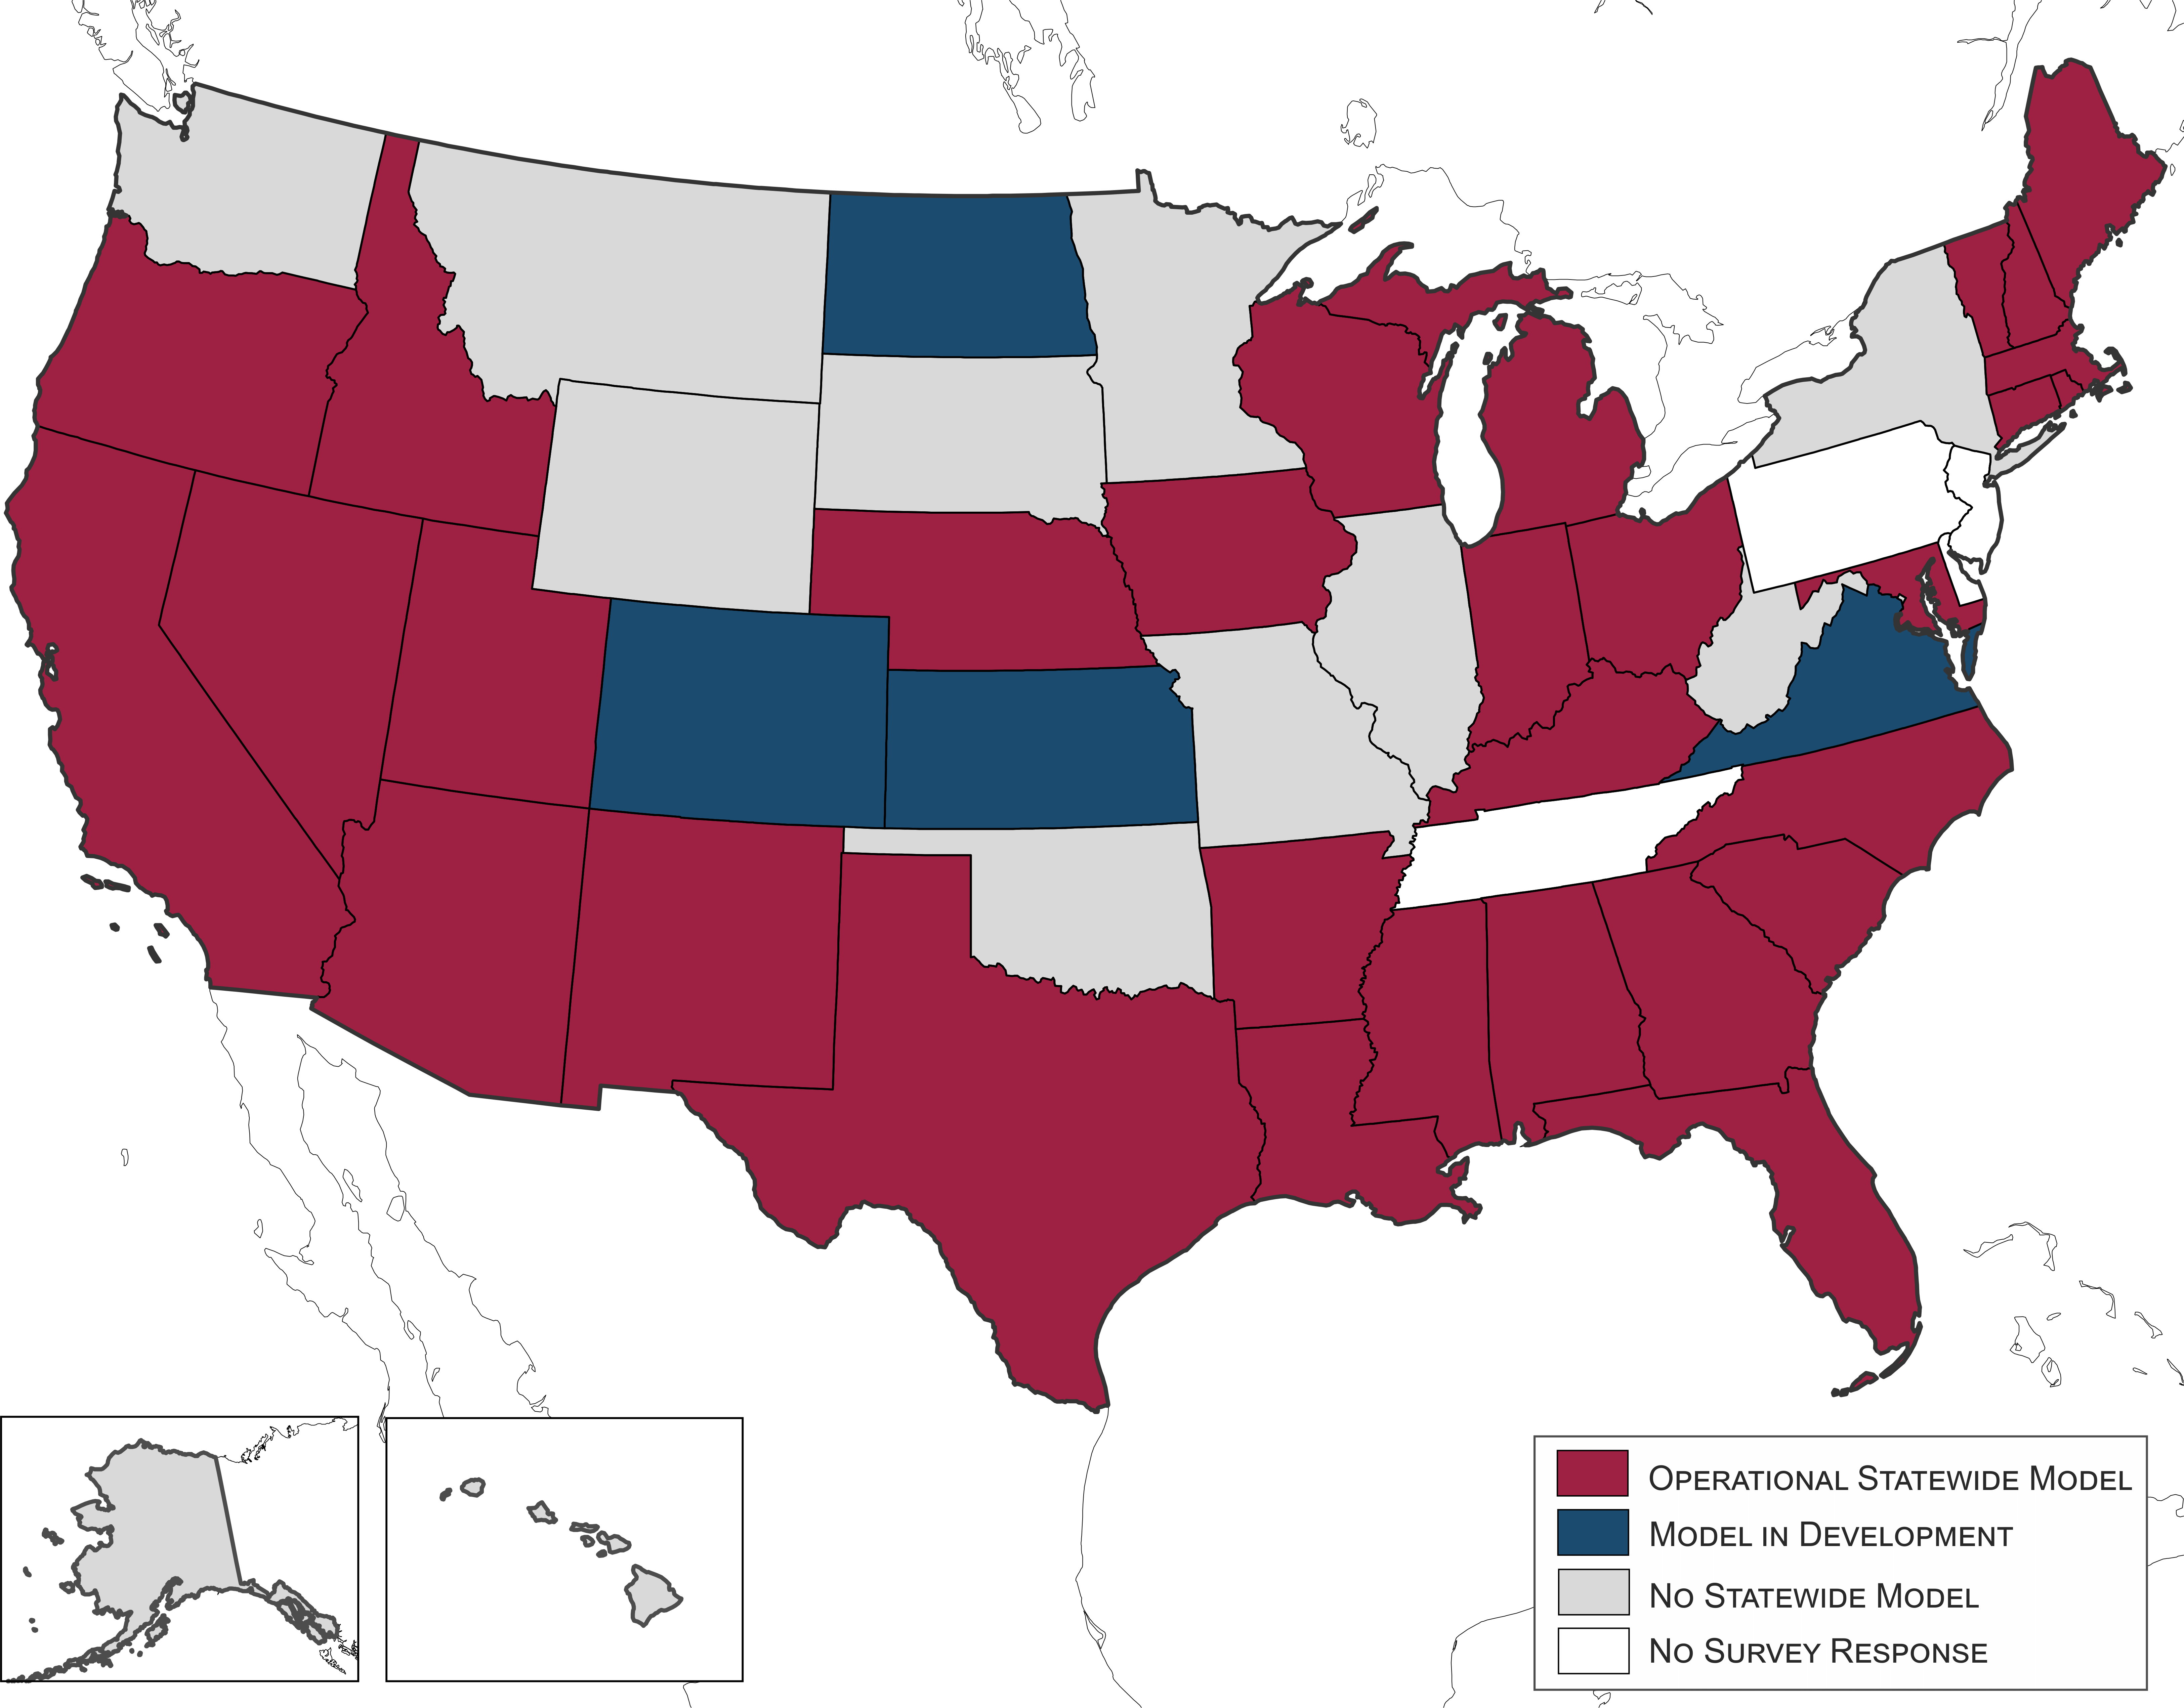
\includegraphics[width=6in]{graphics/01-states-with-operational-models}
\caption{States with operational statewide models}
\label{fig:states-with-operational-models}
\end{figure}

The number of states that responded are summarized in Table \ref{tab:states-conducting}. The response rate was 92 percent. Of the states that responded, 74 percent either operate or are developing a statewide model.

\begin{table}  % 1
\centering
\caption{States conducting statewide modeling}
\label{tab:states-conducting}
\begin{tabular}{lcl}
\hline
Response category & Number of states & Percent \\
\hline
Invited to participate in survey & 50 & 100 \\
Responded & 46 & 92 (of all U.S. states) \\
\hline
Operate a statewide model & 30 & 66 (of states that responded) \\
Developing a statewide model & 4 & 9 (of states that responded) \\
All others & 12 & 12 (of states that responded) \\
\hline
\end{tabular}
\end{table}

The survey also revealed that many states have developed add-on models that support the transportation model. Fifteen states operate separate long-distance travel models, 28 states have some form of freight model, nine states model environmental impacts, and two states formally model land use changes. The survey results are presented in detail in Chapter \ref{sec:survey-existing-practice}.

\subsection{TRB statewide modeling subcommittee survey}

The formal survey was supplemented by an informal survey of members of TRB's subcommittee on statewide modeling, conducted during May 2016. The members of the subcommittee are leaders in the development and application of statewide models, with members from state and federal government, academics, and consultants engaged in this type of work. The following open-ended questions were posed to the subcommittee members and friends:
\begin{enumerate}
\item What are the most important analytical issues that you have recently used statewide models to evaluate? How suitable were the tools and data for the task? Did you encounter any noteworthy issues or challenges? 
\item What emerging trends or issues have decision-makers asked you for help evaluating, but for which your model was not up to the task for? In the same vein, what new questions do you expect to be hit with in the near future?
\item What data, methodological, and institutional barriers are holding statewide modeling back?
\end{enumerate}

Three email replies were received, and eight additional interviews were conducted by telephone or during the TRB Innovations in Travel Modeling conference in early May 2016. The small number of responses precluded tabulation, although each conveyed substantial information. Their insight was illuminating, and certain themes and issues came to light. The analytical issues facing statewide modelers (Question 1) varied widely, resulting in the extensive list shown in The evaluation of projects with multi-jurisdictional impacts was the most frequently cited, followed closely by statewide transportation plan development and prioritization.

Most of the respondents felt that their current models were adequate, suggesting the diversity of modeling approaches described in Chapter \ref{sec:survey-existing-practice} can usually address the specific needs of each client. They likely feel less inclined to update their modeling platforms to more advanced models, given the adequacy of existing models for their needs. The considerable momentum towards activity-based models in congested urban areas has only rarely carried over to statewide modeling, in part because most states appear to lack the resources required to do so.

\begin{table}  % 2
\centering
\caption{Frequently cited issues studied with statewide models}
\label{tab:frequent-issues}
\begin{tabular}{|l|}
\hline
Evaluation of projects with multi-jurisdictional impacts \\
Statewide transportation plan development \\
Statewide project ranking and prioritization \\
High-speed rail feasibility studies \\
Major corridor studies \\
Impact of economic downturn on travel patterns \\
Modeling travel patterns outside of MPO modeled areas \\
Understanding truck flows and origin-destination patterns \\
Network continuity and resiliency analyses \\
Assessment of infrastructure degradation and disruptions \\
Assessing potential for truck-rail diversion \\
Provide inputs to economic impact or environmental models \\
Likely increases in VMT attributable to lower fuel prices \\
Analysis of weight-miles taxes and other demand-based revenues \\
Disinvestment (abandoning or curtailing infrastructure maintenance) \\
\hline
\end{tabular}
\end{table}

The largest reported challenges included:

\begin{itemize}
\item
The lack of precision in the model for detailed corridor studies was often cited. Stated differently, the same levels of spatial, temporal, and behavioral resolution found in urban models were desired at the statewide level. However, stretching an urban model to cover an entire state is impractical and too costly to build and maintain in most cases.
\item 
A lack of data on visitors and their travel patterns was often cited as a significant limitation for some project or corridor studies.
\item 
Too much time went into the development of some models, and too little into the user interface and visualization of model results. This made the models more difficult to use than their urban cousins, although it was acknowledged that many of the latter suffer from the same limitations.
\item 
Coding networks, especially for future years, is very labor-intensive and time-consuming. This was particularly an issue when analysts were asked to include all the capacity or operational improvements across a larger state.
\end{itemize}

The three most common emerging issues identified (Question 2) revolved around the expected benefits of big data, development of multimodal project evaluation or cost-benefit analysis processes, and the likely effect of autonomous and connected vehicles. It is hoped that big data, in the form of passively collected origin-destination patterns and travel times from cellular devices, will fill data gaps at an affordable price point, particularly for freight and commercial vehicle flows. Some viewed this as adding value to traditional revealed and stated preference surveys, while others felt that it opens the door to new modeling approaches.

Some states use a formal economic impact framework, such as TREDIS, in project evaluation, while others are still working on potential approaches. A recent survey of such models by \cite{holian16}, which suggests the use of ad hoc methods until better solutions become available, was also cited.

Modeling the effects of autonomous and connected vehicles is a hot topic at this writing, for which the respondents felt unprepared to address. How to formulate forecasts for a society where such vehicles dominate, and travel choices change in response to them, remain open questions. \cite{issac16} summarizes the likely policy impacts, as well as describing a range of different futures, depending on how society, laws, markets, and governments respond to this new mode of transportation. Beyond her work, however, there appears to be little to guide planners seeking to understand the likely impacts of autonomous vehicles, which respondents expect to be profound.

The largest challenges (Question 3) cited included the difficulty in attracting and retaining well-qualified staff, sporadic or uneven funding for statewide models, the difficulty of integrating or reconciling them with urban models, and the burden of obtaining information about regional or national travel affecting their state. All but one of the respondents felt that the staffing issue was the biggest challenge associated with statewide modeling. Most modelers are classified in pay grades too low to attract well-qualified applicants, forcing agencies to rely upon consultants, contract employees, or sometimes partnerships with MPOs, to gain access to the talent required to build and use such models.

The remaining challenges were cited only a few times, so perhaps less easy to characterize as broad issues. Inadequate funding for travel forecasting is often cited, but is not a problem unique to statewide modeling. The need for better integration of statewide models is a compelling issue that is described further in \S\ref{sec:urban-statewide-integration}. Recent federal data and modeling initiatives that can provide a compelling solution for statewide models are discussed further in \S\ref{sec:national-model-integration}.

\section{Megaregions}

The purpose of this Synthesis Report is to review both statewide and megaregional models. The two are similar in concept, both covering larger regions than urban travel demand models, often with a special focus on long-distance travel and freight flows. In some cases, statewide models and megaregional models may cover a very similar study area. Florida and Arizona are examples where much of the statewide modeling region is often considered one megaregion at the same time. The Texas statewide model covers a region even larger than the Texas Triangle megaregion (Houston-San Antonio-Dallas/Fort Worth).

On the other hand, there are two subtle yet significant differences between statewide and megaregional models, making it worthwhile to explore them separately. First, megaregions commonly ignore jurisdictional boundaries. Even the Florida and Arizona megaregions --- whose extent resembles their respective state boundaries --- do not follow jurisdictional delineations exactly. Some megaregions, such as the Northwestern region from Portland, Oregon to Vancouver, British Columbia or the Midwest megaregion around Chicago and Detroit, even reach across country boundaries into Canada. A megaregional perspective adds the potential to include all parts that functionally belong to a megaregion irrespective of administrative boundaries, yet it also poses the challenge of including stakeholders from different jurisdictions. The second difference between megaregional and statewide models is that the former tend to include fewer rural area and focus much more on the urban cores and their suburbs. Most megaregions focus on large metropolitan areas that are linked together economically or culturally, and rural parts are commonly are left out as the hinterland. Statewide models, in contrast, always cover at least the entire state area, and thereby, include rural and urban areas regardless of economic or cultural linkages.

\subsection{Definition of megaregions}

Megaregions across the Unites States have been analyzed for decades. The Boston-Washington corridor, the Chicago Metropolitan Region, and the Los Angeles Basin are prime examples of frequently studied megaregions \citep{florida08}. In Europe, one early megaregional concept, the Blue Banana, covers an arc stretching from Manchester in Northern England to Milan in Northern Italy. The Blue Banana was later rejected as being too simplistic (as it also covered the highly rural Alps). The European Grape was proposed as an alternative \citep{kunzmann01}, where every single grape abstracted a different European megaregion.

Formal megaregional arrangements are rare, even though political borders do not confine regional interactions and associated impacts. One notable quasi-megaregional agreement in the U.S. is the I-95 Corridor Coalition, a group of transportation agencies and toll authorities along the U.S. East Coast from Maine to Florida. However, being a volunteer and consensus-driven organization the Coalition is limited to actions that support the interests of all players involved. Similarly, the I-10 Coalition including the four states Arizona, California, New Mexico, Texas focuses on facilitating goods movements across this corridor. The Coalition focuses on a very specific topic, namely east-west freight flows of trucks. The Arizona Department of Transportation Director John Halikowski summarized the purpose as ``Someday we want the I-10 Corridor to be filled with truck platoons and connected vehicles, weigh-in-motion sensors and automated truck parking lots'' \citep{adot16}. Megaregional organizations with executive power do not exist in the U.S. to date.

On the other hand, megaregions comprise the economic engine of the U.S., are forecasted to contain half the nation's population growth, and perhaps up to two-thirds of its economic growth by 2050 \citep{amekudzi07}. Supporting the megaregions' economic competitiveness domestically and abroad is a key concern given increasing global competition and international trade. A primary justification for addressing policy issues at the megaregional scale as opposed to the metropolitan scale is that regional economic activities are increasingly linked. Economic shocks to one metropolitan area result in spillovers, both positive and negative, to adjacent metropolitan areas. Consequently, the resulting environmental and social impacts associated with such activities similarly spill across metropolitan areas. Furthermore, as pointed out by \cite{christaller33}, \cite{losch54}, and \cite{ross09b}, individual cities are part of larger systems that are linked by intercity trade hierarchies.

Megaregions are defined in multiple ways in the literature. Half a century ago, \cite{gottmann61} wrote a seminal book of the Northeastern Seaboard reaching from Washington to New York City, the largest urban conglomeration in the world at that time. An update was published by \citep{gottmann90}, in which the megaregion remained mostly defined by population densities. A more common approach, adopted by the U.S. Census Bureau and Bureau of Economic Analysis, is to define regions in terms of labor market commuting sheds, where most workers commute to locations within them for employment purposes. This approach is consistent with the \cite{hoover95} concept of a ``nodal'' region, and Fox and Kumar's (1994) ``functional economic areas,'' where regional activities are oriented towards an internal nodal commercial business district, and there is a presumption of dominance of the node over the surrounding peripheral area \cite{dawkins03}. \cite{richardson78} extends this concept to allow for polycentric regions with several nodes and several peripheries, a concept embodied in the U.S. Census Bureau's current definition of a Combined Statistical Area (CSA).

The definitions proposed by recent authors differ in terms of the units of analysis that make up the underlying regions and how they are connected. The \cite{rpa06}, along with urban planning graduate students from the University of Pennsylvania, identified ten megaregions in the U.S. They characterized them as interconnected along at least one of the following dimensions: (1) environmental systems and topography, (2) infrastructure systems, (3) economic linkages, (4) settlement patterns and land use, and (5) shared culture and history. \cite{hagler09} proposes quantitative criteria to establish these linkages. An index was created with points assigned to counties based upon whether the county was part of a core-based statistical area, had a population density exceeding 200 persons per square mile, and had increases in population, employment, or population densities exceeding certain thresholds. \cite{ross08} proposed the following procedure to identify megaregions: (1) identify the core areas, (2) identify the boundaries of the areas of influence, (3) apply local characteristics, and (4) finalize the boundaries.

FHWA has shown an increasing interest in studying megaregions over the past decade. \cite{ross09c} wrote a seminal report on the delineation of megaregions. Their proposed delineation of ten megaregions across the country is shown in Figure \ref{fig:ross-megaregions}. America 2050, a Regional Plan Association's~national infrastructure planning and policy program, has defined similar yet slightly different megaregions \citep{rpa06}, but the concept is similar. Common criteria for megaregions are economic ties, commute linkages, and cultural identities.

\begin{figure}[!tb]
\centering
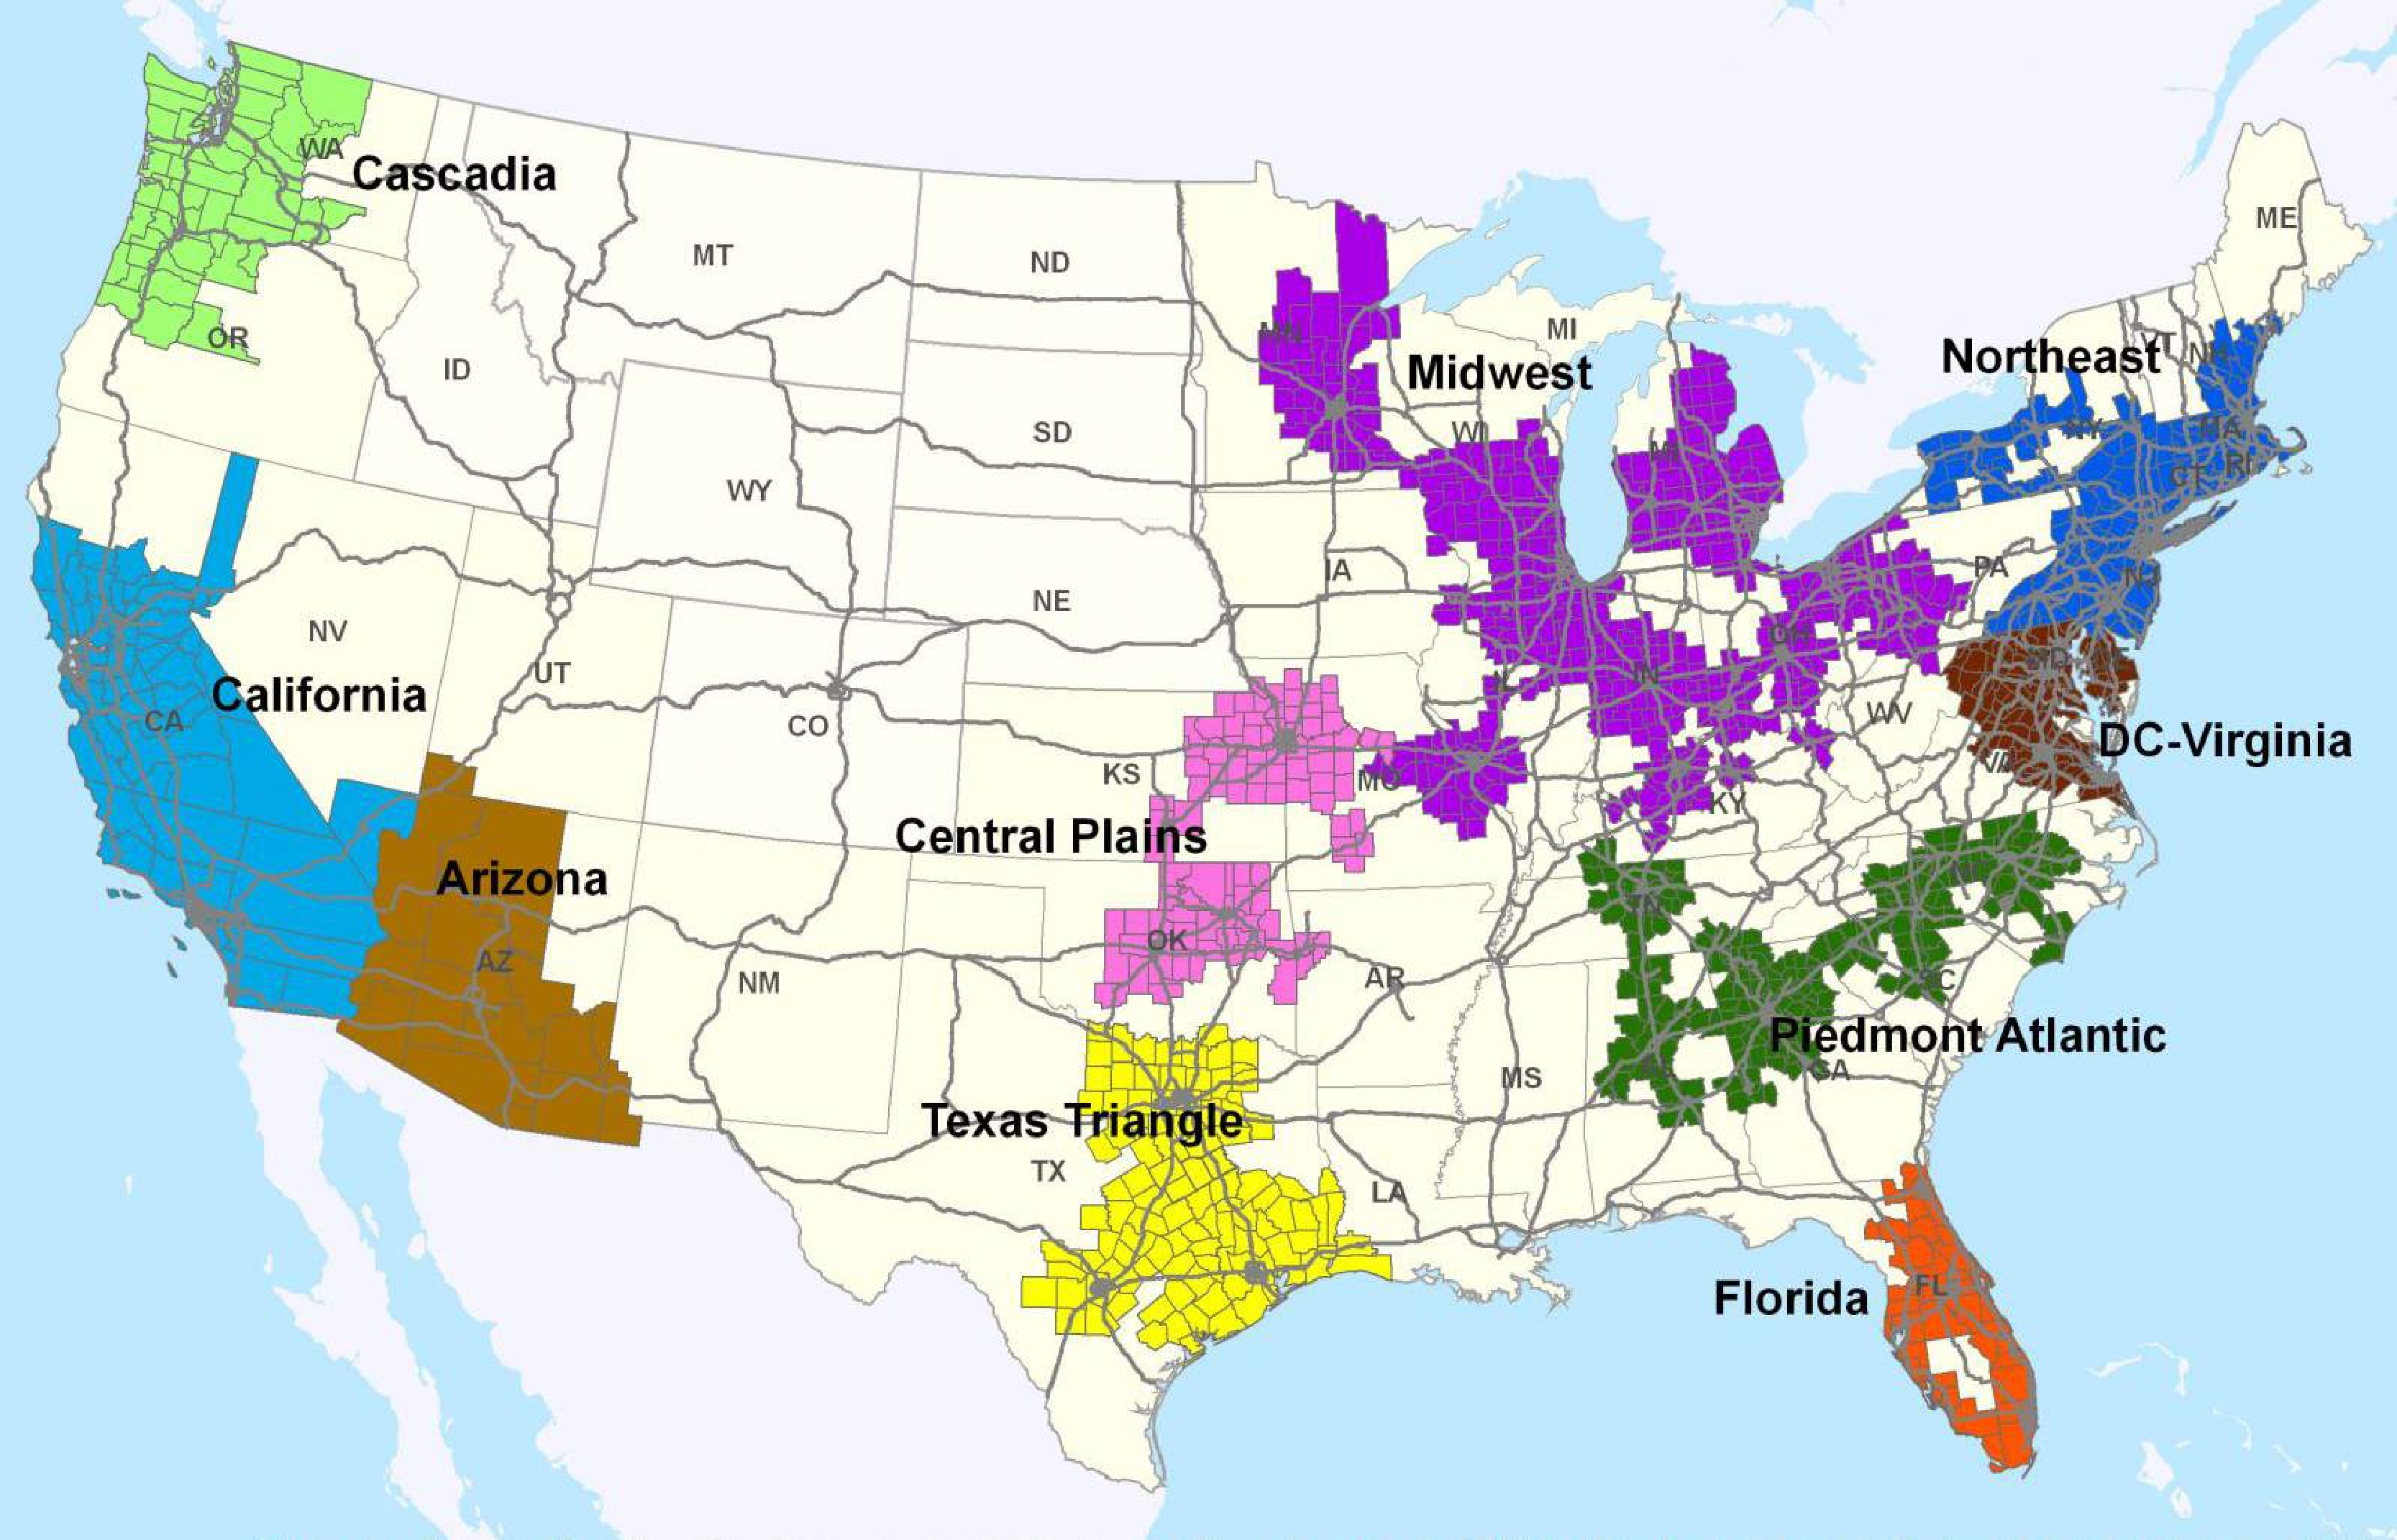
\includegraphics[width=6.5in]{graphics/02-megaregionsAccordingToRoss2009}
\caption[Delineation of ten megaregions in the U.S.]{Delineation of ten megaregions in the U.S. (Source: \cite{ross09b})}
\label{fig:ross-megaregions}
\end{figure}

In 2015, FHWA initiated an internal working group with representatives from several states and universities to foster megaregional analyses and activities. The five key interests of this working group are (in no particular order) freight, safety, economic vitality, infrastructure/transportation and environmental issues, all of which directly relate to transportation issues studied in megaregional models. The aim of the workgroup is to implement some form of an institution for each megaregion. However, the definition of institutions is left to the local jurisdictions to decide. Governance approaches for megaregions are not proposed by FHWA at this time. Nevertheless, FHWA helps to raise the awareness of the importance of megaregions and create synergies between agencies within megaregions.

FHWA also set up an online information system to support analyses on megaregions \citep{fhwa16a}. Under the category Megaregion Research, this website offers interactive maps that may be used to visualize 13 megaregions (as currently defined by FHWA) and compare them with the locations of MPO boundaries, highway networks, county population, GDP by MSA, truck volumes, among others.

For the time being, megaregions will be issue-based. Quasi-governmental structures to promote megaregions at large are not expected to be implemented soon. Problems that require joint action, such as highway corridors, rail corridors, protection of larger ecosystems or providing affordable housing, may lead to ad hoc creations of megaregional agencies with limited authority and under the tight control of state and/or metropolitan jurisdictions.

\subsection{Megaregional transportation models}\label{sec:megaregion-transport-models}

While there is a substantial body of literature on analyzing megaregions, little research has been conducted on modeling megaregions. The Chesapeake Bay Megaregional Model was implemented for the Washington, D.C. megaregion \citep{moeckel15b} as a FHWA demonstration project, and is described in more detail in \S\ref{sec:chesapeake-bay-megaregion-model} (page \pageref{sec:chesapeake-bay-megaregion-model}). As there are no institutionalized megaregional governance structures in place, there is no agency requesting continuous development of megaregional models. Existing models have been either issue-based (compare \S\ref{sec:hsr-megaregions}) or research-driven. Outside of federal initiatives, it is unlikely that megaregional models are built, maintained and applied.

While there are 29 operational statewide models plus five statewide models under development, only four megaregional models have been recently developed in the U.S. One is the Chesapeake Bay model described above. The remaining three are ad hoc models developed for specific purposes:
\begin{itemize}
\item \cite{zhang13} developed a model at the megaregional scale, but it is only intended for hurricane evacuation analysis of several southern states. The model focuses on the assignment step and models congestion depending on the areas needing evacuation if a hurricane is approaching.
\item A five-state model encompassing Texas and four neighboring states was built to evaluate interstate passenger rail corridors between them \citep{meyer15}. It provided analyses for the Southwest Multi-State Regional Plan, but does not appear to have been used otherwise.
\item Several statewide models are being fused to support analyses for the Appalachian Development Highway System Economic Analysis Study \citep{edrg16}. Details of the model are not yet available, but understood to represent synthesis and reconciliation of forecasts developed using several statewide models, and development of traffic assignment capabilities, rather than the development of a true megaregional model.
\end{itemize}

Outside the U.S., the Netherlands National Model System (NMS), often referred to by its Dutch name Landelijk Model Systeem (LMS), models travel demand for the entire Netherlands \citep{gunn94}. The SASI (Spatial and Socio-economic Impacts of Transport Investments and Transport System Improvements) models interactions of the economy with the transportation system for the entire European Union \citep{wegener08}. However, infrastructure benefits are only represented through accessibilities, which do not capture actual congestion on the transportation network.

Because of the limited number of existing megaregional models, this report clearly focuses on statewide modeling. Given the similarities in large-scale modeling, megaregional models are covered as a sibling of statewide modeling. With the recognition that the economic, social and environmental systems happen at the megaregional scale, unobstructed by municipal, county, MPO, or state boundaries, formal megaregional institutions with legislative power may be implemented in the future.

Many aspects of statewide modeling discussed in this report will apply to megaregional models as well. While one might argue that megaregions cover larger areas than states, the largest statewide models in operation (California and Texas) cover already a population and area larger than any megaregion in the U.S. The most important difference between megaregional and statewide modeling is that the former in most cases cover parts of several states, making it more challenging to reconcile input data and agree on issues that need to be addressed with the model.

\subsection{High-speed rail and megaregions}\label{sec:hsr-megaregions}

High-speed rail (HSR) has perhaps quietly become the most compelling case for megaregion modeling. New systems have been proposed in California, Florida, and Texas, whose statewide model coverage might be adequate for systems operating wholly within them. However, for other systems under consideration, the relevant markets cover multiple states, and their potential connections to existing intercity rail and air systems might involve even broader regions. Indeed, the potential for HSR seems to be one of the fundamental features used to define megaregions \citep{florida09, ross09b}.

All the known operational HSR models in North America are designed expressly for studying such systems. At most, they are one-way adaptations of existing statewide models, whose finished work does not appear to benefit the original model. In California, for example, the HSR Authority uses a modeling system that is separate from the California statewide model, as described in \S\ref{sec:california-hsr-model} (page \pageref{sec:california-hsr-model}). The former has taken advantage of data collected by the latter, but they remain otherwise separate works. In Texas, the statewide model was used to develop an inter-regional HSR model and forecasts. While data used to build the latter would certainly be useful in the evolution of the former, there are no known plans to integrate the two models. The first-generation Oregon statewide model was used to quickly examine the feasibility of HSR along the upper Pacific Coast, but the initiative never proceeded to formal study, which likely would have spawned the development of a custom model.

The development of separate HSR models seems to be more of tactical necessity than a long-term trend. In its defense, HSR forecasting requires more robust and sophisticated mode choice modeling than found in all but a handful of statewide models. The need to model the competitive response of air carriers, risk and uncertainty, and accuracy requirements exceed the capabilities of any known statewide or megaregion model. The Federal Railroad Administration also has unique analytical requirements at the preliminary, intermediate, and final stages that further influence the data and tools used to assess HSR ridership \citep{sdg11}.

Once built there would seem to be few impedances to using an HSR model as the first generation of a megaregion model. While it would need to be expanded to cover the many markets not addressed by HSR models, or at least not at the same level, many of the data used in their development would seem more broadly applicable. Due to the lack of megaregional governance structures discussed in \S\ref{sec:megaregion-transport-models}, however, such conversion from an HSR to a megaregion model has not occurred yet. Outside the specific interest (HSR), no agency has picked up such models for further analysis in different domains.


\chapter{Rationale for statewide modeling}\label{sec:rationale-for-statewide-modeling}

Statewide modeling is undertaken to inform a wide variety of policy analysis, planning, investment, and programming activities. The range of reported uses is described in this chapter. It is divided into three parts. The first part describes the primary uses of statewide models, with an emphasis on how they differ from metropolitan (or urban) models. The evaluation of the impacts of State Long-Range Transportation Plans (LRTP) is perhaps the most common application of statewide models. The second part describes scenario analysis conducted with statewide models, and provides insights from the survey on the types of scenarios predominantly analyzed. Finally, the third part deals with performance measures in statewide modeling.

\section{Motivations for statewide modeling}

Statewide models are used to analyze the impact of policies and trends that are implemented or addressed by state governments, but not captured with urban or national models. This includes several travel markets not commonly included or underrepresented in urban models:

\begin{itemize}
\item
Foremost, statewide models capture travel occurring in areas outside of major metropolitan areas. Smaller MPOs and agencies outside of them often do not operate their own transportation models, yet there is a need to analyze transportation planning in these areas as well. In practice, state DOTs commonly fulfill this role using statewide models.
\item
Metropolitan transportation models cannot capture travel between MPOs. For example, the three MPOs in Arizona --- the Maricopa Association of Governments (MAG) in Phoenix, Sun Corridor Metropolitan Planning Organization in Pinal County, and Pima Association of Governments (PAG) in Tucson --- share borders and have substantial travel between them. However, their models focus on travel within each area. A statewide model is used to fully represent travel demand in the corridor between Phoenix and Tucson. Similar examples include travel between the San Diego and Los Angeles areas, or between Baltimore and Washington, D.C. Statewide models have been developed to capture travel between these areas.
\item
Long-distance travel is of concern in statewide models. MPO models commonly represent travel with origins or destinations outside their MPO area as external trips. They enter or leave at external stations, which do not distinguish between final destinations two miles versus two thousand miles away. Both ends of such trips are often explicitly represented in statewide models, which is necessary given the size of study areas for most states. There is no universal definition of long-distance travel. The National Household Travel Survey (NHTS) defines long-distance travel as trips with 50 miles or more, and the older American Travel Survey (ATS) as 100 miles or more. Long-distance travel behavior differs substantially from short-distance travel, which is why most statewide models explicitly distinguish between them. The former is infrequent, with different destinations (more concentrated in city centers of major metropolitan areas), a mix of modes different from local travel, different hours during the day (less focused on morning and evening peak hours), and different path choices. Long-distance travelers have traditionally tended to stay on highways and major arterials, for they are not as familiar with local streets. However, this tendency is reduced by the use of navigation systems.
\item
Freight is a key market represented in most statewide models. Twenty of the 34 states that operate or are developing statewide models include short-distance truck flows, and 26 model long-distance truck flows explicitly (59 and 76 percent, respectively). Most urban models capture truck flows as well, but many of them travel outside of the modeled area, necessitating their representation in statewide models. Freight moving by rail, water, and air are irrelevant in urban models, apart from where they transfer to trucks. With larger study areas for states, these modes become more important. Accordingly, 13 states (or 38 percent) have implemented explicit freight mode choice models.
\item
Statewide models can provide external traffic volumes for urban models. In many cases, urban models prefer to use traffic counts at external stations and distribute those volumes between internal zones and other external stations using gravity models. Using a statewide model for this purpose, however, offers two significant advantages. First, the statewide model explicitly distinguishes between origins and destinations that are internal to the MPO region from those that are external. This lead to a better distinction between through, internal-to-external, and external-to-internal trips, rather than relying upon under-specified gravity models to make this distinction. Secondly, using statewide model forecasts for urban models allows accounting for the impact of scenarios that may affect traffic flows outside the MPO area. For instance, a major highway project within an MPO region may affect the routing of long-distance trips with origins and destinations outside of it. Running this scenario in the statewide model first to generate updated external volumes, and then with the MPO model using these revised external volumes, will create consistency between long and short-distance travel.
\end{itemize}

Some states also develop ``officially sanctioned'' datasets and forecasts using statewide models. Consistent zonal socioeconomic datasets and --- even more challenging --- forecasts provide data that states can work with and refer to. Traffic counts sometimes are mapped to statewide model networks, providing a common reference system used across agencies within a state. In the same vein, statewide models may also be tools that facilitate cooperation between different agencies.

%\protect\hypertarget{h.ra3igdrh8psb}{}{}
At the same time, it is also important to recognize what statewide models are not well suited for. There are no known domain reasons why statewide models cannot be used for certain analyses. Rather, insufficient spatial and temporal resolution in statewide models may be an impediment to analyzing scenarios that are more commonly addressed using urban models. For example, most statewide models are too coarse to adequately represent non-motorized travel (i.e., walk or bike). The impact of transit-oriented development is another example that requires higher spatial resolution around transit stations than commonly found in statewide models. Likewise, impacts of very small projects, such as a new highway ramp, tend to be overlooked by statewide models for lack of spatial resolution. Statewide models also tend to be less capable of representing detailed and complex urban transit systems, even though the Google Transit Feed Data (discussed further in Chapter \ref{sec:emerging-methods-opportunities}) may overcome this limitation for statewide models to some degree.

\section{Scenario analysis}\label{sec:scenario-analysis}

Statewide and megaregional models are built to test scenarios to advise policy-makers. Such scenarios may include:

\begin{itemize}
\item
\emph{Infrastructure scenarios} test the impact of new infrastructure, such as the extension of a road, the implementation of a new transit line, or the development of additional housing in a specific location. These scenarios refer to changes in the built environment. They may also include scenarios of disinvestment, such as abandoning or curtailing infrastructure maintenance.
\item
\emph{Policy scenarios} test the impact of alternative policies to handle transport, such as raising tolls on a highway link, prohibiting trucks from using selected roads, or increasing the frequency of transit service. Policy scenarios test alternative regulations that could be actively implemented by a jurisdiction without significantly changing the built environment.
\item
\emph{Global scenarios} test the impact of uncertain future developments, such as increased immigration, rising energy prices or widespread adaptation of autonomous vehicles. Changing conditions tested in global scenarios usually cannot be influenced by local policy makers, but are rather given as an exogenous constraint the region must adopt. These scenarios are commonly used to understand the range of impact, such as testing different levels of them on congestion (Figure \ref{fig:immigration-vs-congestion}).
\end{itemize}

\begin{figure}
\centering
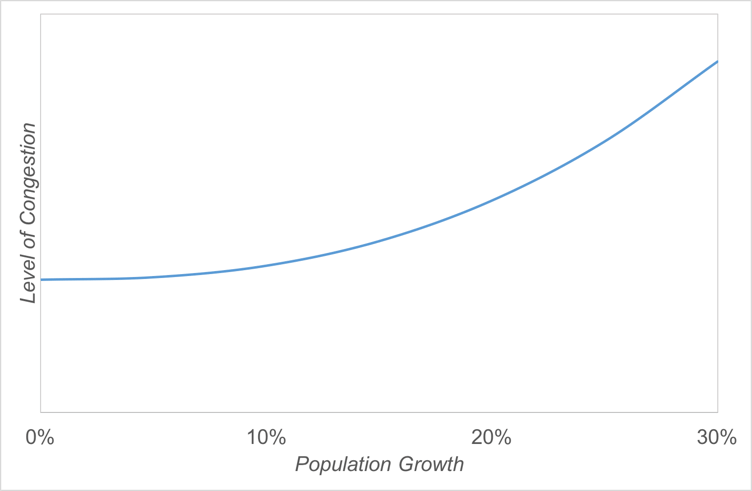
\includegraphics[scale=0.4]{graphics/03-immigration-vs-congestion}
\caption{Hypothetical relationship between immigration and level of congestion}
\label{fig:immigration-vs-congestion}
\end{figure}

Often, models are developed with specific applications in mind. For example, it was imperative that agricultural flows, which change by season, were represented realistically in Idaho's Statewide Model. The Maryland Statewide Model was built predominantly to test highway scenarios that apply to areas outside of the Baltimore and Washington metropolitan areas. Sensitivity to changes in zoning was a key design feature of Oregon's Statewide Model.

The survey asked explicitly for what kind of scenarios were evaluated using statewide models. Respondents could select more than one answer, which is why the total of all responses is much larger than the number of states that operate statewide models. A summary of the common scenarios is shown in Figure \ref{fig:typical-scenarios}. Light bars indicate scenarios described as most important.

\begin{figure}  % 4
\centering
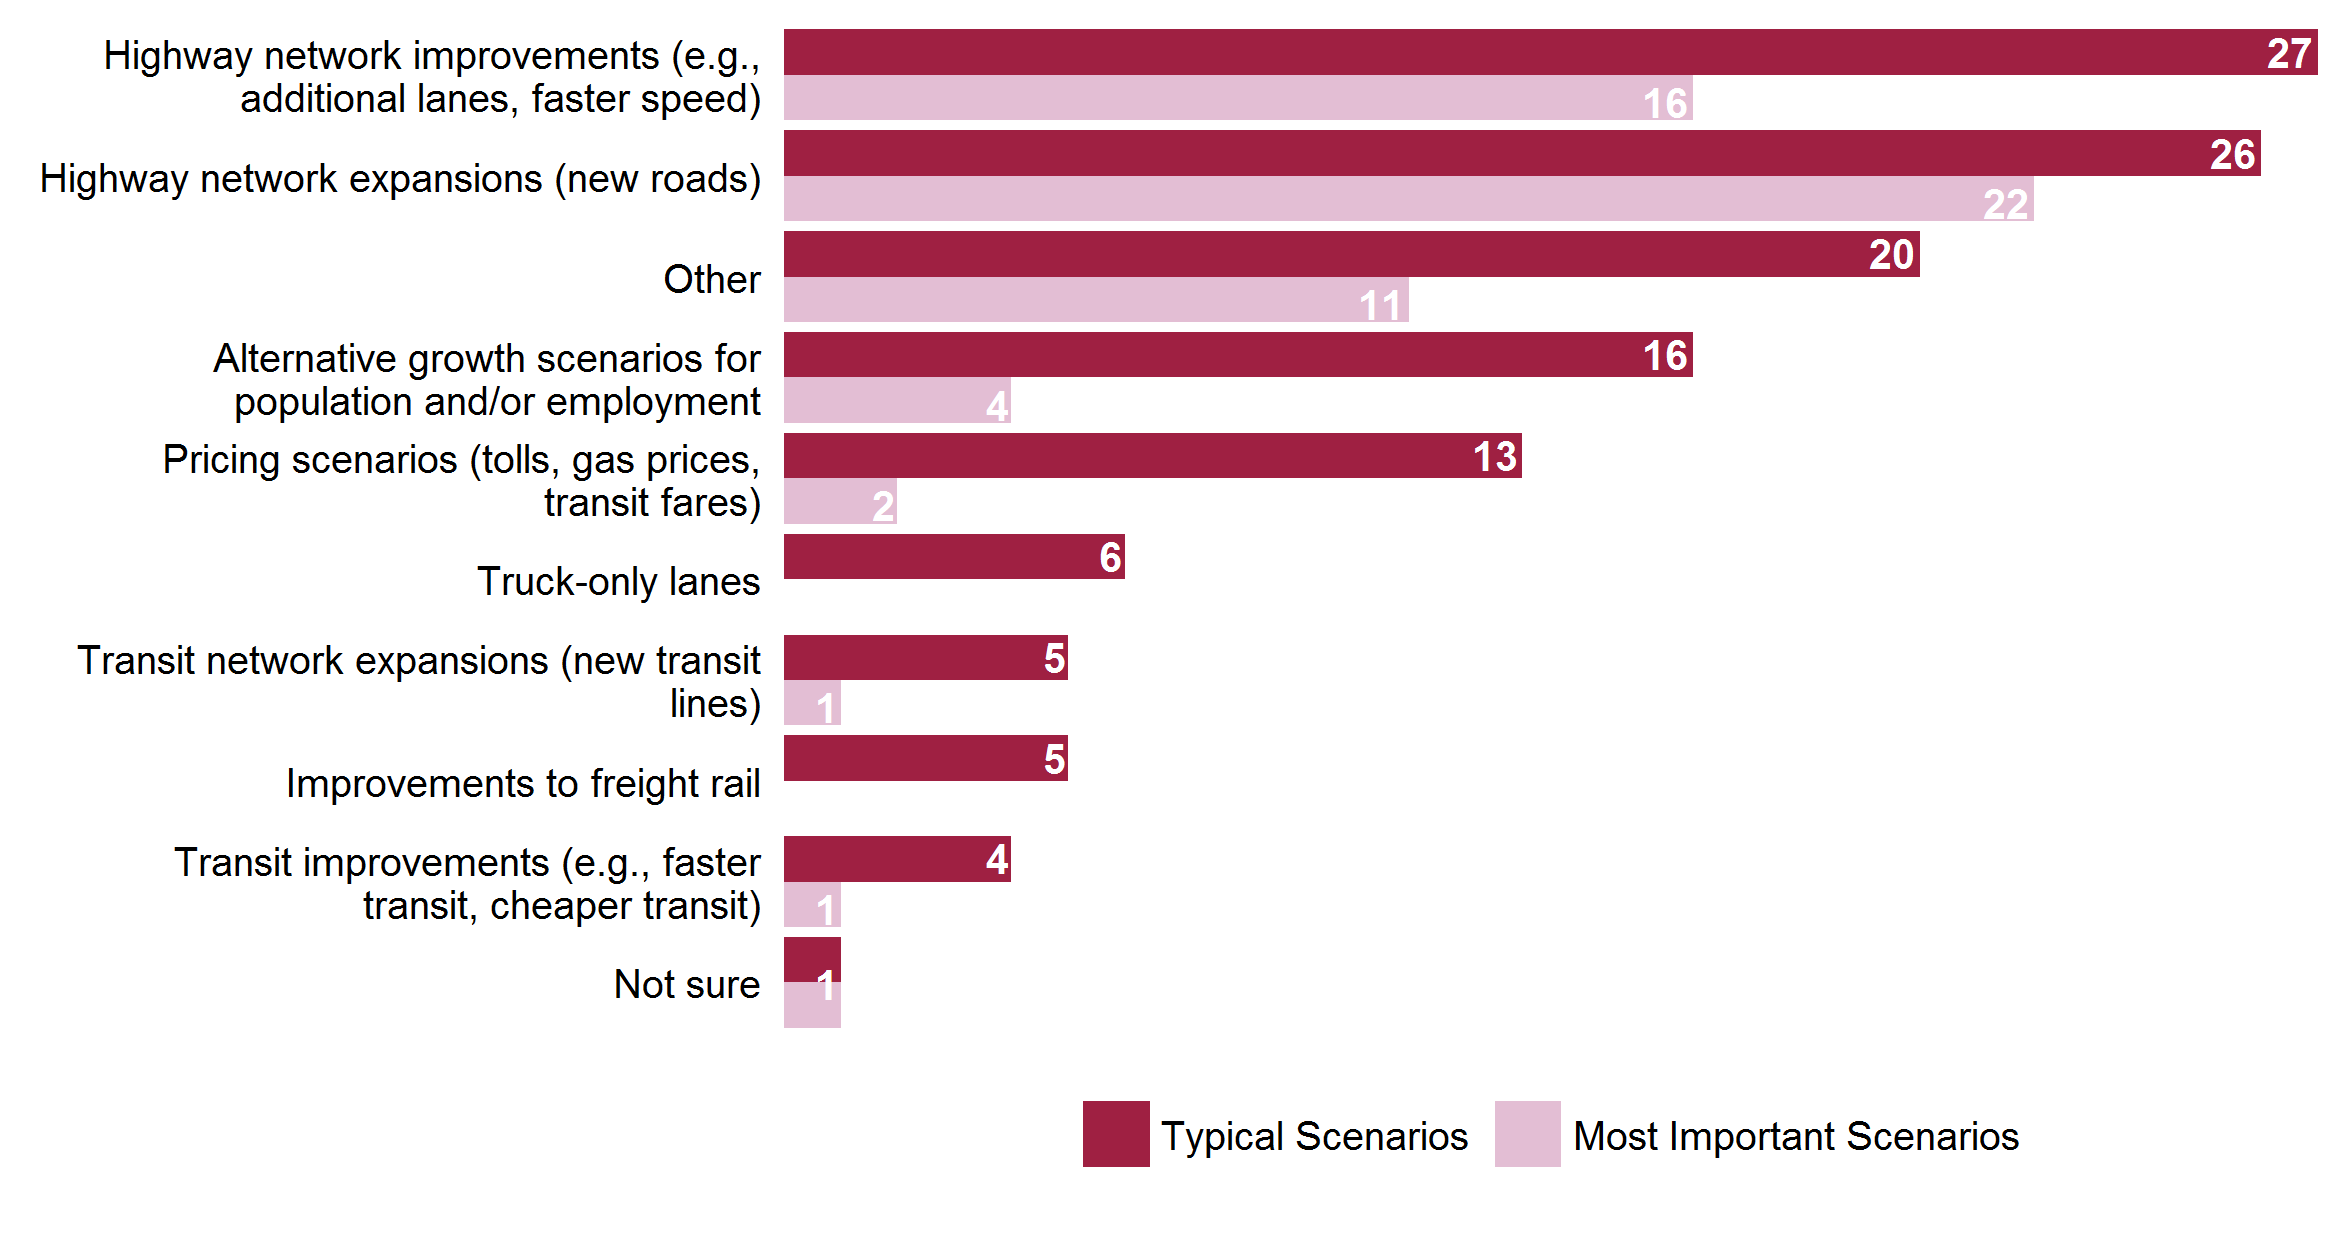
\includegraphics[width=6in]{graphics/04-typical-scenarios-tested}
\caption[Typical scenarios tested with statewide models]{Typical scenarios tested with statewide models (multiple answers allowed)}
\label{fig:typical-scenarios}
\end{figure}

By far the most common application of statewide models (27 respondents, or 79 percent) involved testing of highway network improvements, including additional lanes, change of speed and similar network enhancements. Testing the impacts of network additions (i.e., the construction of entirely new roads) was a close second. This was not surprising, as state and local governments together spend six times as much on highways as they spend on transit \citep{usdot14}. The next most important scenario type was global scenario testing of the impact of alternative population growth rates. Sixteen of the 34 states that conduct statewide modeling (47 percent) reported using statewide models to test alternative growth forecasts. This finding underlines the large uncertainties associated with population and employment forecasts. States can assess the viability and resilience of their transportation system under a variety of alternative futures.

Pricing scenarios (including tolls, gas price increases and transit fares) were tested by 13 states (or 38 percent of states that conduct statewide modeling). The interest in and necessity of testing alternative pricing structures is on the rise, as lack of alternative forms of funding pushes transportation agencies to charge for the use of infrastructure \citep{perez12}. As such, it is rather surprising that only slightly more than a third of states with models test pricing scenarios. A possible explanation might be that pricing strategies are more predominant in local jurisdictions. Tolled highway infrastructure, such as Interstate Turnpikes, tend to be administered by commissions that are independent of state DOTs, often operating separate models.

A few states listed ``Other'' scenarios relevant to them. Four states (Kentucky, Maine, Michigan and Vermont) specifically added that they use the statewide model to analyze road closure for highway construction and maintenance. Texas and Utah pointed out that they use their statewide models to analyze freight. Indiana and Nebraska use the statewide model for subarea analyses and select link analyses, which allows identifying traffic volumes and trip origin and destinations in a selected part of the state or on individual links. Oregon also used their statewide model to analyze the impact of weight-restricted bridges, seismic impacts, and economic impacts of various levels of investment. Massachusetts also used their model for air quality conformity analysis. Florida conducts evacuation analyses. Five case studies are described in more detail in Chapter \ref{sec:case-studies}, with a special focus on the type of applications these models are used for.

\section{Performance measures}

Assessing changes in performance measures under different scenarios is an important use of state\-wide models. Such measures evaluate how efficient a transport system operates in terms of consistent metrics, such as reliability and travel time delay and variability. Even though not written specifically for modelers, a good overview of performance measures commonly used by transportation planning agencies is provided in NCHRP Report 618 \citep{cambridge08}. Statewide models are commonly expected to provide similar outputs to ensure that the models can be used to evaluate performance measures under various scenarios. Performance measures are often categorized by four dimensions:

\begin{itemize}
\item Duration, or how many hours the delay on the network lasts
\item Extent, or how many people or vehicles are affected
\item Intensity, or by how much travel time is delayed, and
\item Variability, describing whether the congestion pattern is similar every day (such as expected peak hour congestion) or irregular (such as delays caused by incidents)
\end{itemize}

Travel demand models are reasonably strong at predicting the second and third dimensions, but inherently bad at assessing the first and last issues. Some statewide models only represent daily total traffic, making it impossible to assess the duration of congestion. Several models distinguish four time-of-day periods, which allows only coarse evaluation of congestion duration. Runtimes of the assignment step tend to be long. Therefore, all statewide models analyzed in this report distinguished four time-of-day periods at most, except for Colorado, where they plan to work with seven to 10 periods. The representation of variability is almost non-existent in statewide models. Such models typically represent an average day rather than the observed variability from one day to the next.

Performance measures that are typically used in conjunction with transportation models commonly include:

\begin{itemize}
\item Travel time in minutes (vehicle-hours traveled)
\item Travel delay in minutes (vehicle-hours delay)
\item Travel distance in miles (vehicle-miles traveled)
\item Travel distance diversion in miles (actual traveled distance under congested conditions minus shortest paths in free-flow travel environments)
\item Average speed
\item Vehicle or traveler throughput
\item Percent of congested segments (miles of network links under congestion divided by total miles of network length)
\item Equity analysis, such as whether certain income groups benefit more from a certain investment than others
\item Gaseous emissions (such as CO\textsubscript{2}, PM, NO\textsubscript{x}) or noise generated, if an environmental impact capability is implemented
\item Economic benefits of investments (often measured as changes in gross domestic product), if economic impact modeling is implemented
\end{itemize}

\noindent Such measures can be expressed as either per traveler, per vehicle, or as a system-wide total.

The Moving Ahead for Progress in the 21st Century Act (MAP-21) required the Secretary, in consultation with States, MPOs and other stakeholders, to establish performance measures in the areas of:

\begin{enumerate}
\item Pavement condition on the Interstate System and the remainder of the National Highway System (NHS)
\item Performance of the Interstate System and the remainder of the NHS
\item Bridge condition on the NHS
\item Fatalities and serious injuries --- both number and rate per vehicle mile traveled --- on all public roads
\item Traffic congestion
\item On-road mobile source emissions
\item Freight movement on the Interstate System
\end{enumerate}

States were required to set performance targets in support of those measures. While MAP-21 did not explicitly call for transportation modeling, statewide models were routinely used to assess at least items 2, 5, 6, and 7. It is thought that these measures will remain important in the more recent Fixing America's Surface Transportation (FAST) Act of 2015.
\chapter{Survey of existing practice}\label{sec:survey-existing-practice}

%\protect\hypertarget{h.2hcxkn16a7yd}{}{}

Statewide modeling is becoming
mainstream in the U.S. In 2005, 20 of the 50 U.S. states had implemented operational statewide models \citep{horowitz06}. The survey conducted in 2016 for this synthesis report revealed that 34 states (out of 46 states that responded in 2016) operate statewide models, an increase of 70 percent over 11 years.

\section{Survey findings}

The survey of state agencies was a key source of information about the state of practice in statewide modeling in the U.S. However, as with any survey, the results reflect how the respondents understood the question, which in some cases may not have perfectly matched its intent. There are likely to be some important nuances and elements of context in all the responses that are impossible to fully capture in a standardized survey. While the discussion in this section represents the state of practice in the U.S. at large, individual responses may have been imprecise due to misunderstanding or limited familiarity with the topic of a question. The difficulties found when summarizing results will be discussed in more detail in \S\ref{sec:survey-critical-review}. Nevertheless, the overall state of practice in statewide modeling is presumed to be represented accurately in this section.

The survey conducted for this synthesis report was divided into eight parts. One of these parts, Scenarios, was already discussed in \S\ref{sec:scenario-analysis} (page \pageref{sec:scenario-analysis}). The following detailed description of survey results follows the structure of the remaining seven principal parts, namely person travel demand model, person long-distance model, freight model, economic model, land use model, environmental impact model, and resources. The chapter will end with some summarizing remarks on survey findings.

\section{Person travel demand modeling}\label{sec:person-demand-modeling}

The survey started with a question about the type of person travel demand model implemented or under development. For the states that distinguish between short and long-distance travel this initial part of the survey referred to short-distance travel only. Many states, however, do not operate a separate long-distance model. For those states, the following answers refer to both short and long-distance travel. The traditional four-step modeling paradigm is applied in 26 states, as shown in Figure \ref{fig:person-model-frequency}. This includes some states that model auto travel only and skip the mode choice step (making it essentially a three-step model with trip generation, trip distribution, and assignment). This category also includes states that split traffic into various periods of time, making it a five-step model. It should be noted, however, that many states apply this four-step concept to short-distance travel only, using a different modeling approach for long-distance travel. Five states are in the process of developing a four-step transportation model. Four other states have an operational activity-based model, with two more states developing such models.

\begin{figure}
\centering
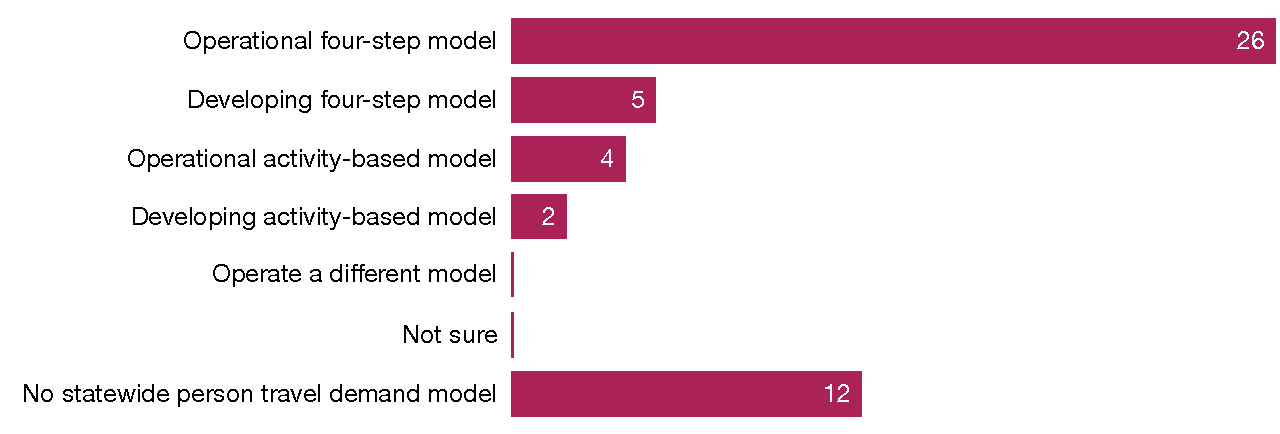
\includegraphics[scale=0.65]{graphics/05-person-demand-model-types}
\caption[Frequency of travel demand model types for person travel]{Frequency of travel demand model types for person travel (multiple answers allowed)}
\label{fig:person-model-frequency}
\end{figure}

The spatial distribution of different model types across the nation is shown in Figure \ref{fig:statewide-modeling-status}. Activity-based models are more common in the Western part of the U.S., with Ohio and soon Maryland being the only two states in the eastern part of the country using them.

\begin{figure}   % 6
\centering
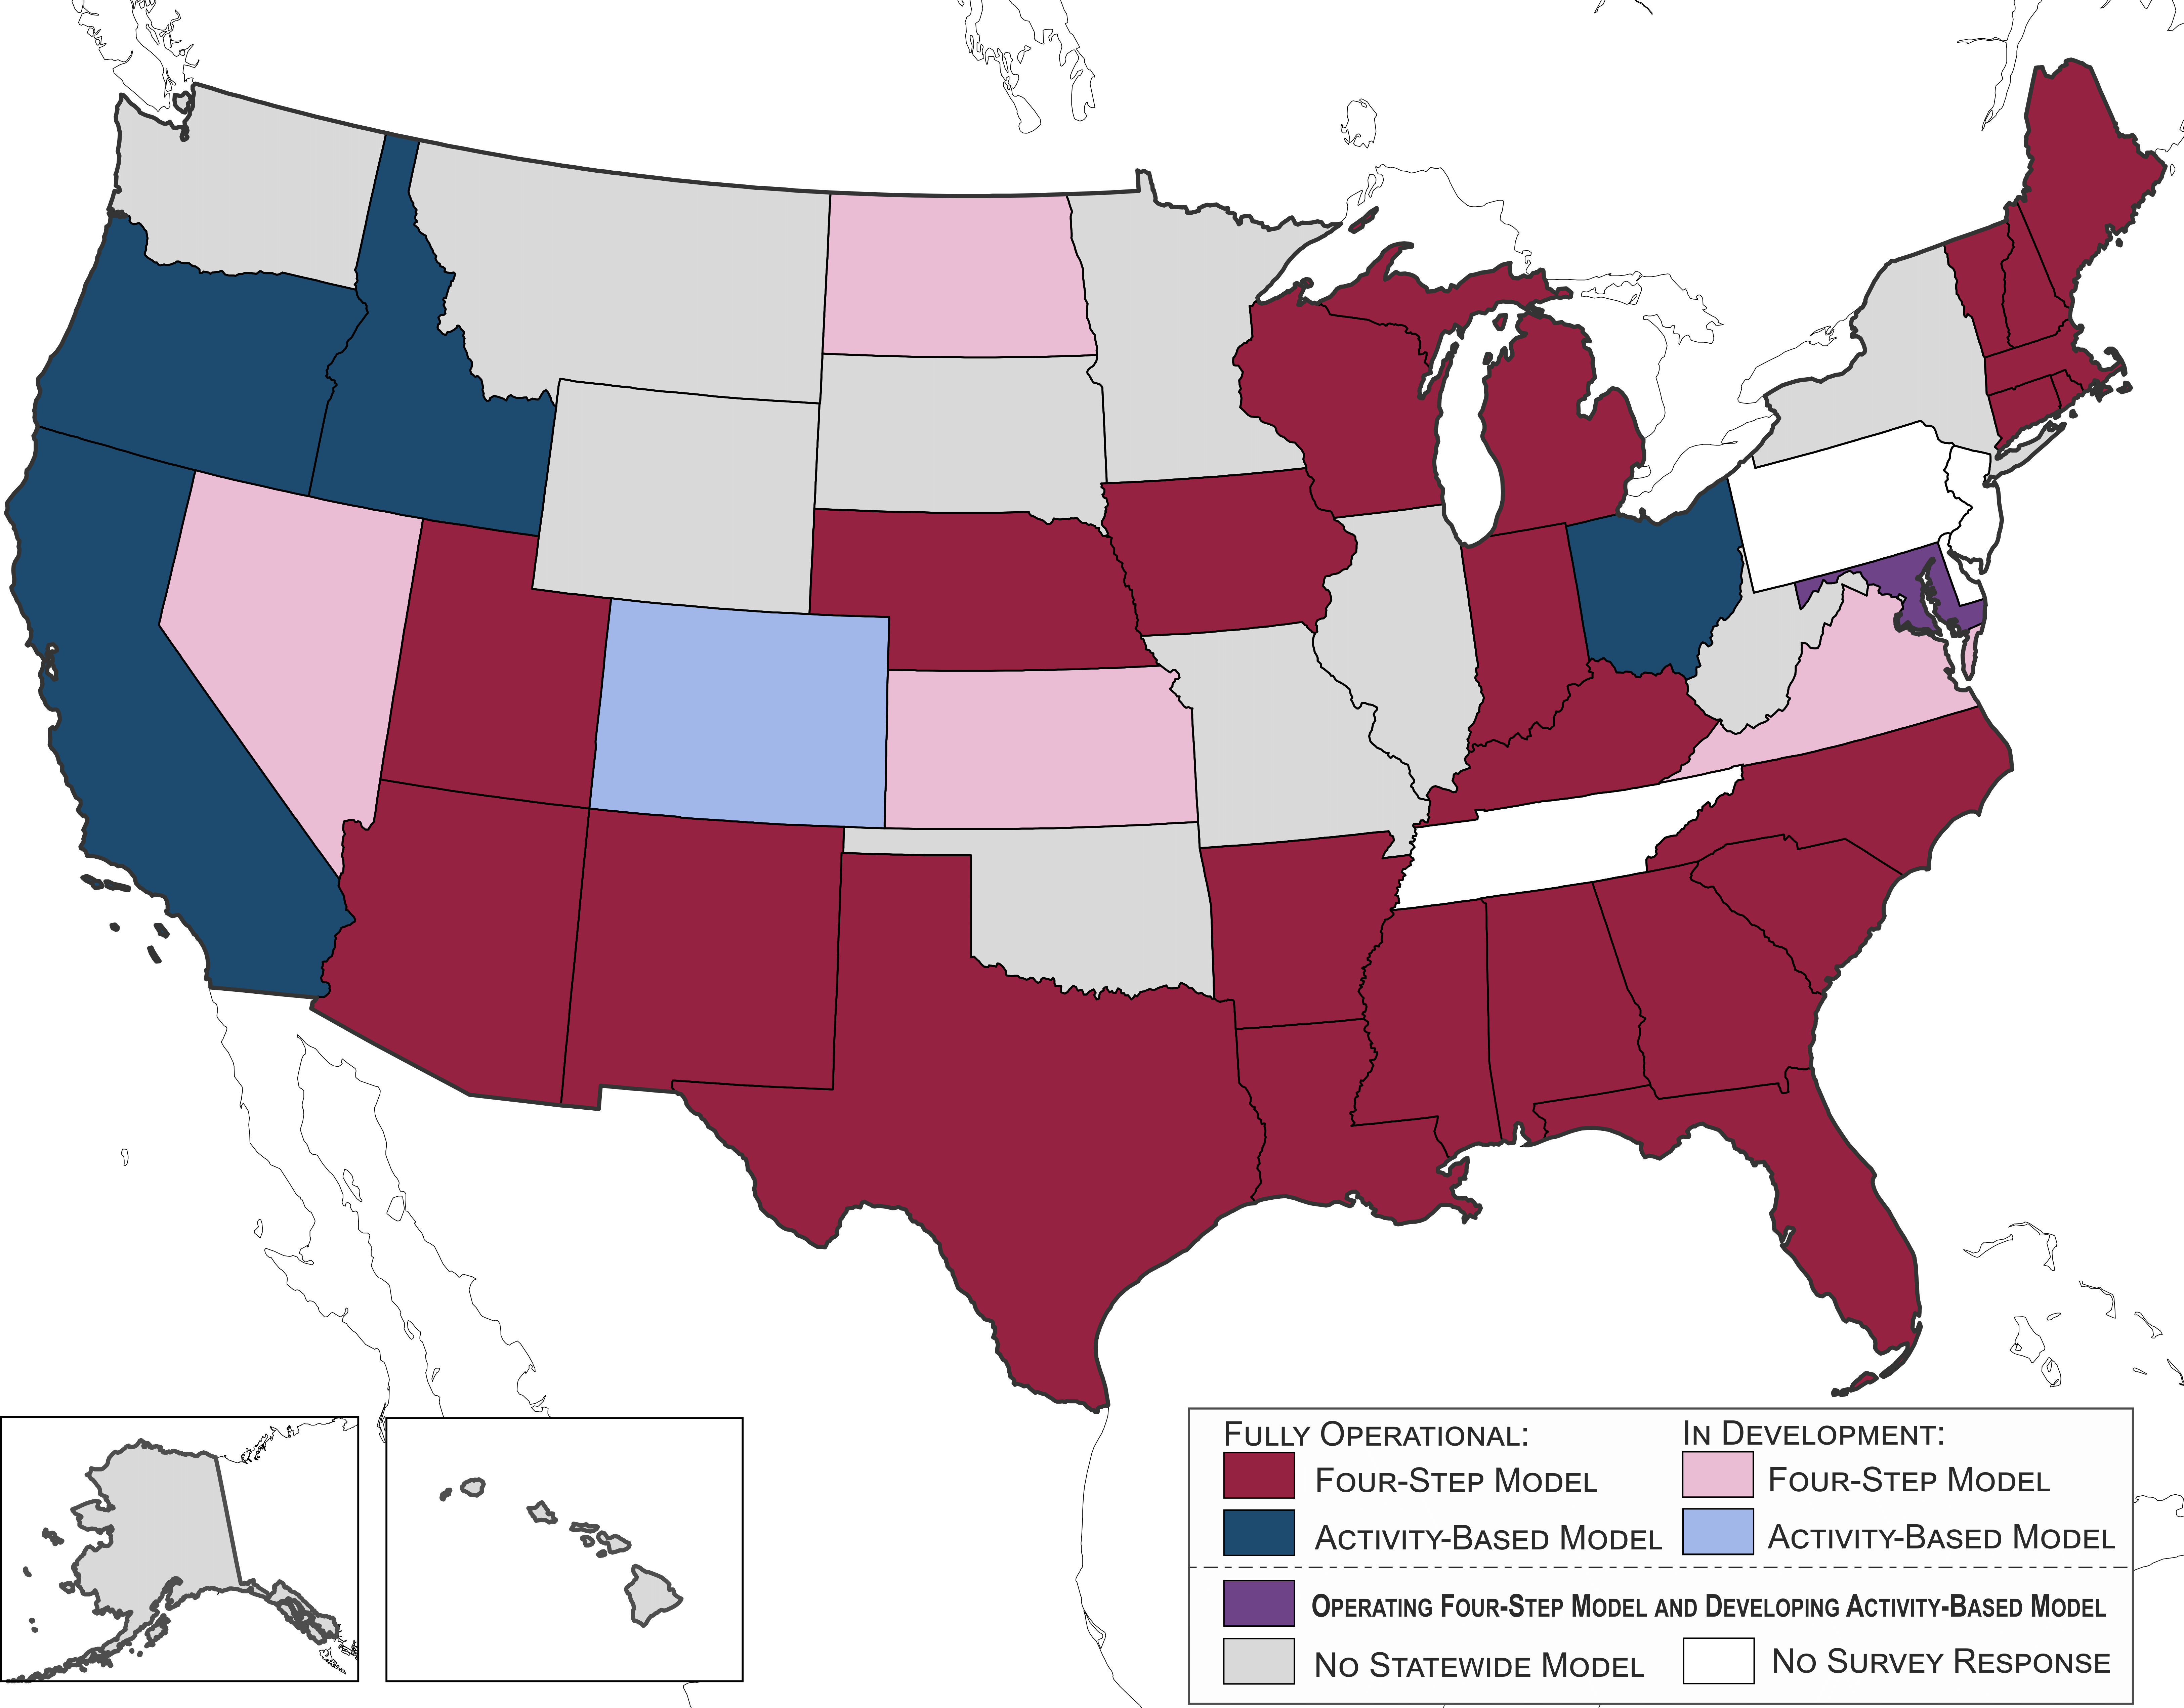
\includegraphics[width=6.5in]{graphics/06-statewide-modeling-status}
\caption{Status of statewide modeling across the U.S.}
\label{fig:statewide-modeling-status}
\end{figure}

Hawaii as an island state does not operate a statewide model. Individual models are implemented for the islands of Kauai, Maui, Oahu and Hawaii, covering over 99 percent of the state's population. Other states without statewide models tend to be clustered towards the northern part of the country in regions with lower population densities and less severe levels of congestion, which probably has affected the need and desire for developing statewide models.

The frequency of trip and tour generation methods is shown in Figure \ref{fig:person-generation-methods}. As expected, using trip rates based on cross-classification is the most common approach. In the early years of travel demand modeling, multiple regression was the dominant approach for generating trips. In multiple regression models, trip rates are treated as continuous rather than discrete variables, which may lead to unrealistically high (or sometimes even negative) number of trips in zones with unusual household type compositions. Therefore, the 1970s marked a shift away from aggregate zonal level regression analysis to more disaggregate household cross-classification procedures \citep{ortuzar11}. However, trip rates based on multiple regression have the advantage of allowing the analyst to consider multiple independent variables, and may work well if resulting generated trips are reviewed carefully for inconsistencies. Kansas and Vermont are even using both methods in trip generation.

\begin{figure}  % 7
\centering
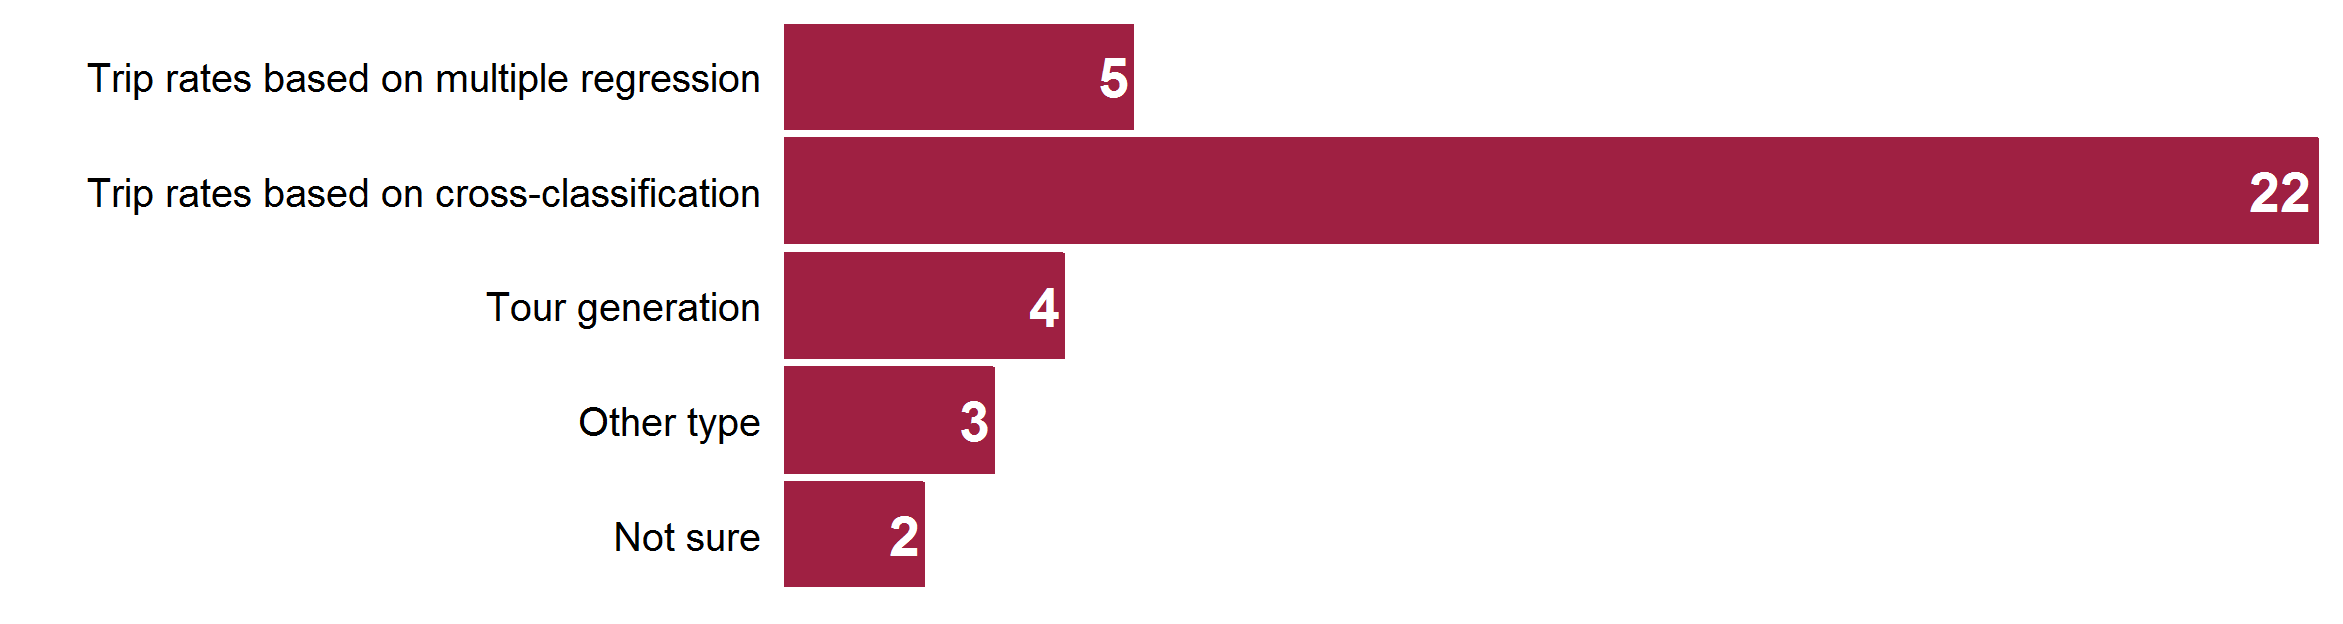
\includegraphics[width=6.4in]{graphics/07-person-generation-methods}
\caption[Frequency of trip and tour generation methods for person travel]{Frequency of trip and tour generation methods for person travel (multiple answers allowed)}
\label{fig:person-generation-methods}
\end{figure}

The fact that cross-classification rates dominate statewide modeling merely reflects the dominance of this approach in the travel demand modeling domain. Colorado models daily activity patterns (as is typically done in activity-based models), and Virginia combines logit models with regression analysis.

Trip distribution shows a strong concentration on gravity models, with 22 states applying this concept (see Figure \ref{fig:person-distribution-models}). This traditional form of trip distribution is borrowed from the physics gravity concept, explaining that the number of trips between two zones is proportional to their size (in terms of population, employment, or the number of trips generated/attracted) and inversely proportional to their distance. This model type is easy to implement and very easy to calibrate, as --- in its simplest form --- only one impedance parameter needs to be adjusted until the observed average trip length is matched by the model. However, if trips with longer distances (such as trips over 50 miles) are included, gravity models become challenging to calibrate because the tail of longer trip lengths cannot be fine-tuned very well in a gravity model with only one impedance parameter. This is less of a concern if a separate long-distance model is used (true for seven states that implemented gravity models for short-distance travel only.

\begin{figure}  % 8
\centering
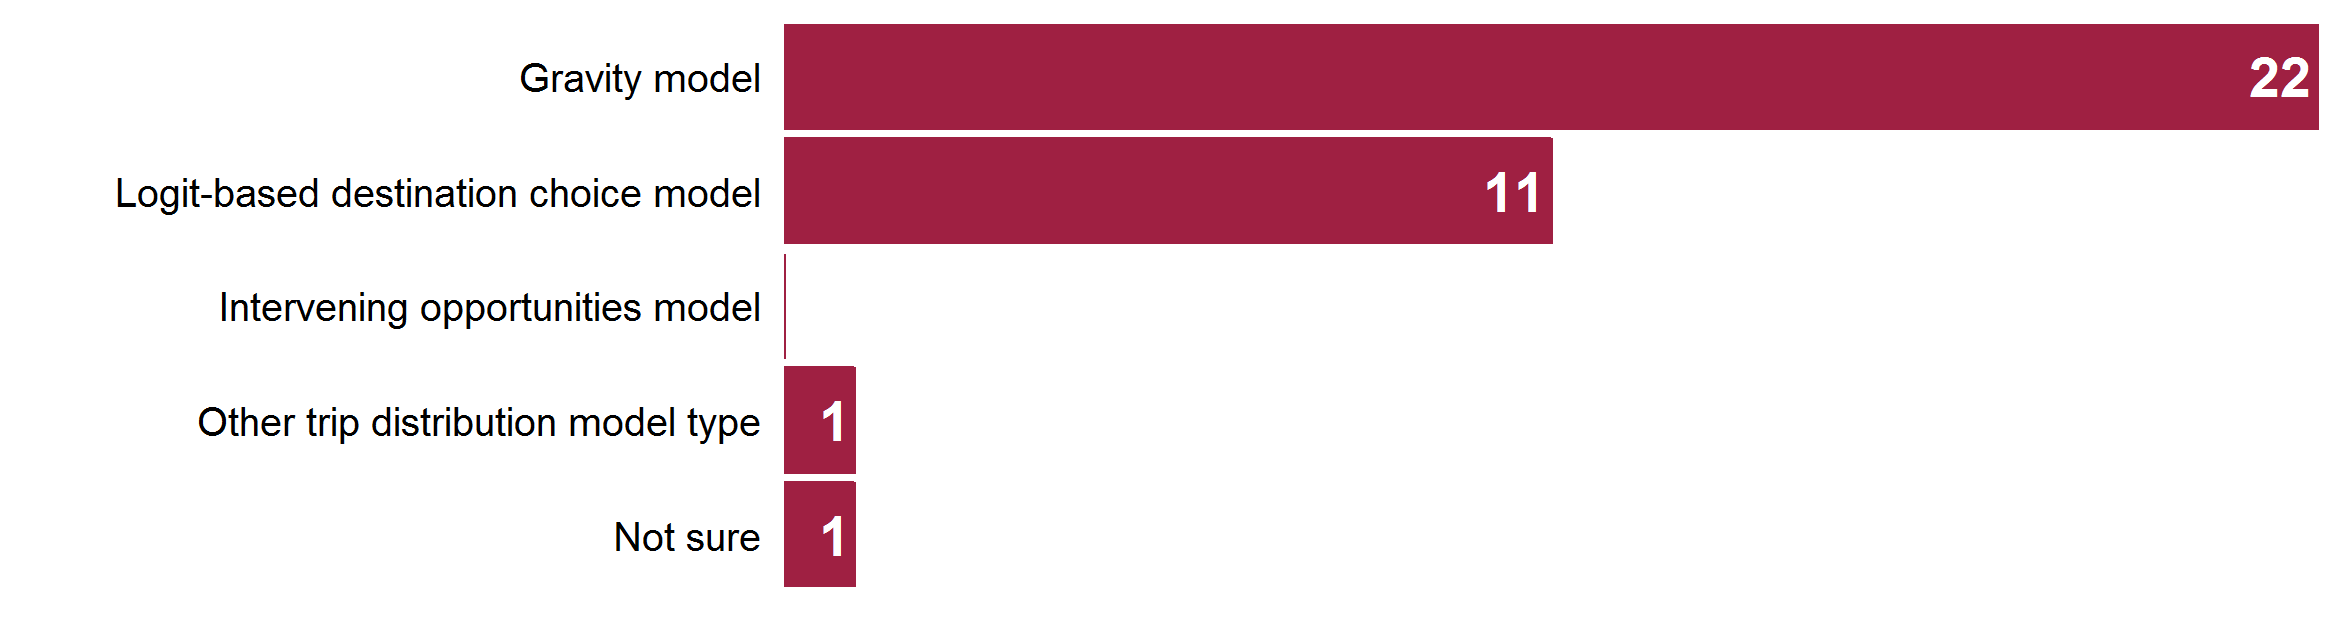
\includegraphics[width=6.4in]{graphics/08-person-distribution-models}
\caption[Frequency of trip distribution models for person travel]{Frequency of trip distribution models for person travel (multiple answers allowed)}
\label{fig:person-distribution-models}
\end{figure}

The logit-based destination choice model, on the other hand, evaluates different destinations against each other, taking into account the attraction in every other zone (measured by socio-economic data or the number of trips attracted), the distance to every other zone, and possibly other factors that may affect destination choice. In the Maryland statewide model, for example, an additional penalty was used to reflect the observed psychological barrier of choosing destinations on the other side of major rivers. 

As shown in Figure \ref{fig:person-distribution-models}, eleven states apply logit-based destination choice models. This includes Ohio, where a logit-based destination choice model is joined with an economic allocation model for work locations. Even though logit-based destination choice models are capable of handling long-distance trips, eight out of eleven states that use logit-based destination choice models have also implemented a separate long-distance travel model. Such a combination commonly ensures the largest model sensitivities for the trip distribution step.

Note that no state is using an intervening opportunities model \citep{stouffer40}, a concept from social sciences that received attention in the 1960s but is no longer common in travel demand modeling.

While early travel demand models ignored mode choice entirely, nowadays about every other statewide model explicitly accounts for mode selection, as shown in Figure \ref{fig:person-mode-choice}. Thirteen states responded that they only generate auto trips, obviating the need for a mode choice model. Furthermore, five states apply static (fixed) modal shares, making it 18 states (or 53 percent) that do not model mode choice. Of the 16 states that do model mode choice, the clear majority use nested logit models, with only two states using simple multinomial formulations. Probit and mixed logit models, sometimes applied in urban travel demand models, are not in use for mode choice modeling in statewide models in the U.S.

\begin{figure}
\centering
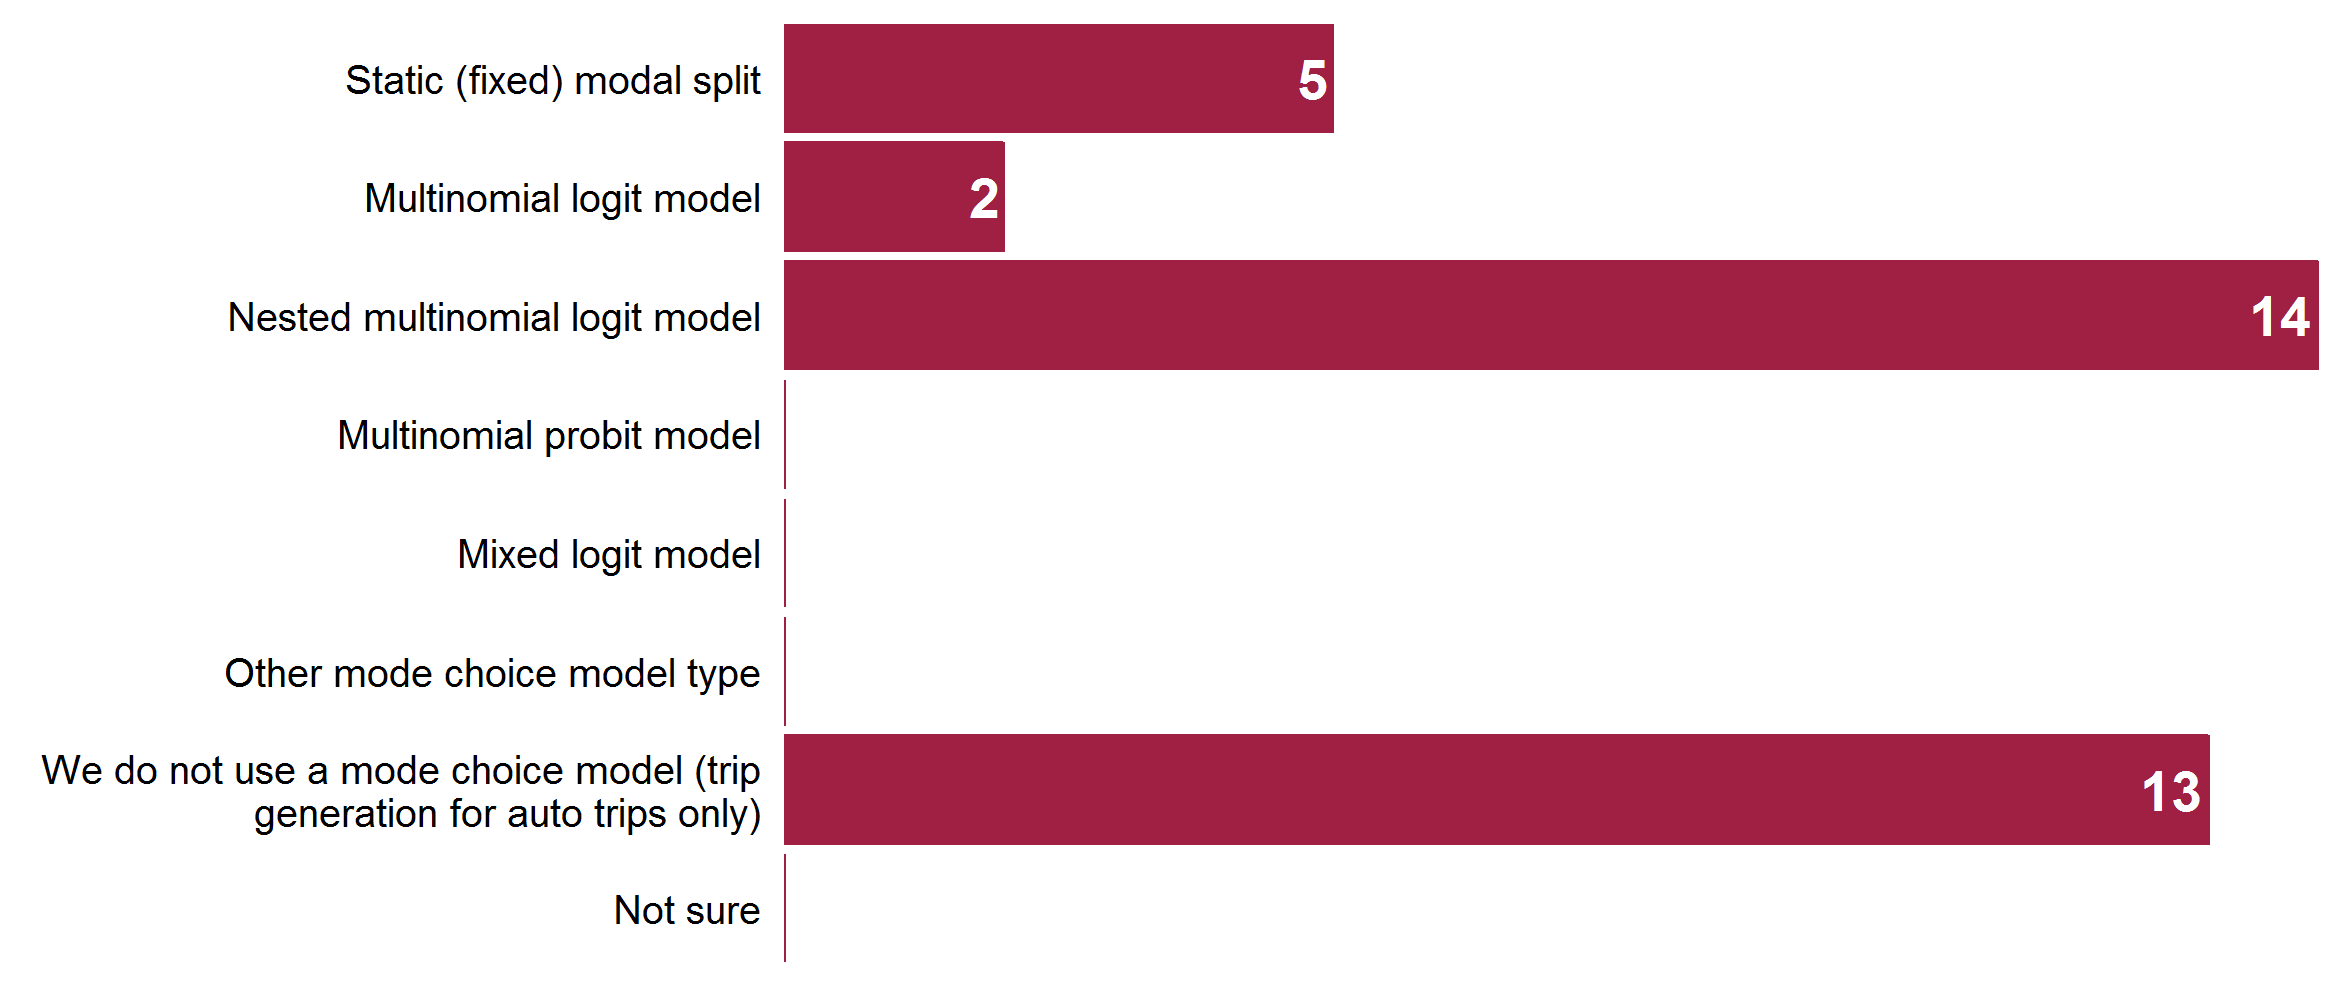
\includegraphics[width=6.4in]{graphics/09-person-mode-choice}
\caption{Frequency of mode choice models for person travel}
\label{fig:person-mode-choice}
\end{figure}

It should be noted that three of the states that do not model mode choice for short-distance travel do so for long-distance trips (North Carolina, Virginia, and Wisconsin). Nevertheless, it is remarkable that many statewide models ignore mode choice. While most scenarios analyzed with statewide models refer to changes of the highway network (see \S\ref{sec:scenario-analysis}), impacts on mode choice may be significant. Increased congestion or higher gas prices are likely to push some travelers from the auto to the transit mode, and vice versa, congestion relief through additional roadway construction may trigger transit riders to switch to the car. This outcome is missed in models without an explicit mode choice model, although possibly less important in non-MPO areas with limited transit options.

The modes of transportation represented in statewide models for person travel are shown in Figure \ref{fig:person-modes-represented}. This graphic includes statewide models that apply static mode shares and mode choice models. All statewide models include auto trips as the dominant mode, analyses of which such models are built for. Thirteen of them distinguish auto occupancy, at least between drive-alone and share-ride. Indiana and Maine split trucks from person travel in the mode choice model, which means (a) that truck trip generation rates were added to person trip generation rates and (b) that the same trip distribution was applied for person travel and trucks. Virginia aggregates all transit modes into one choice for transit. Colorado has a separate mode for school buses.

\begin{figure}  % 10
\centering
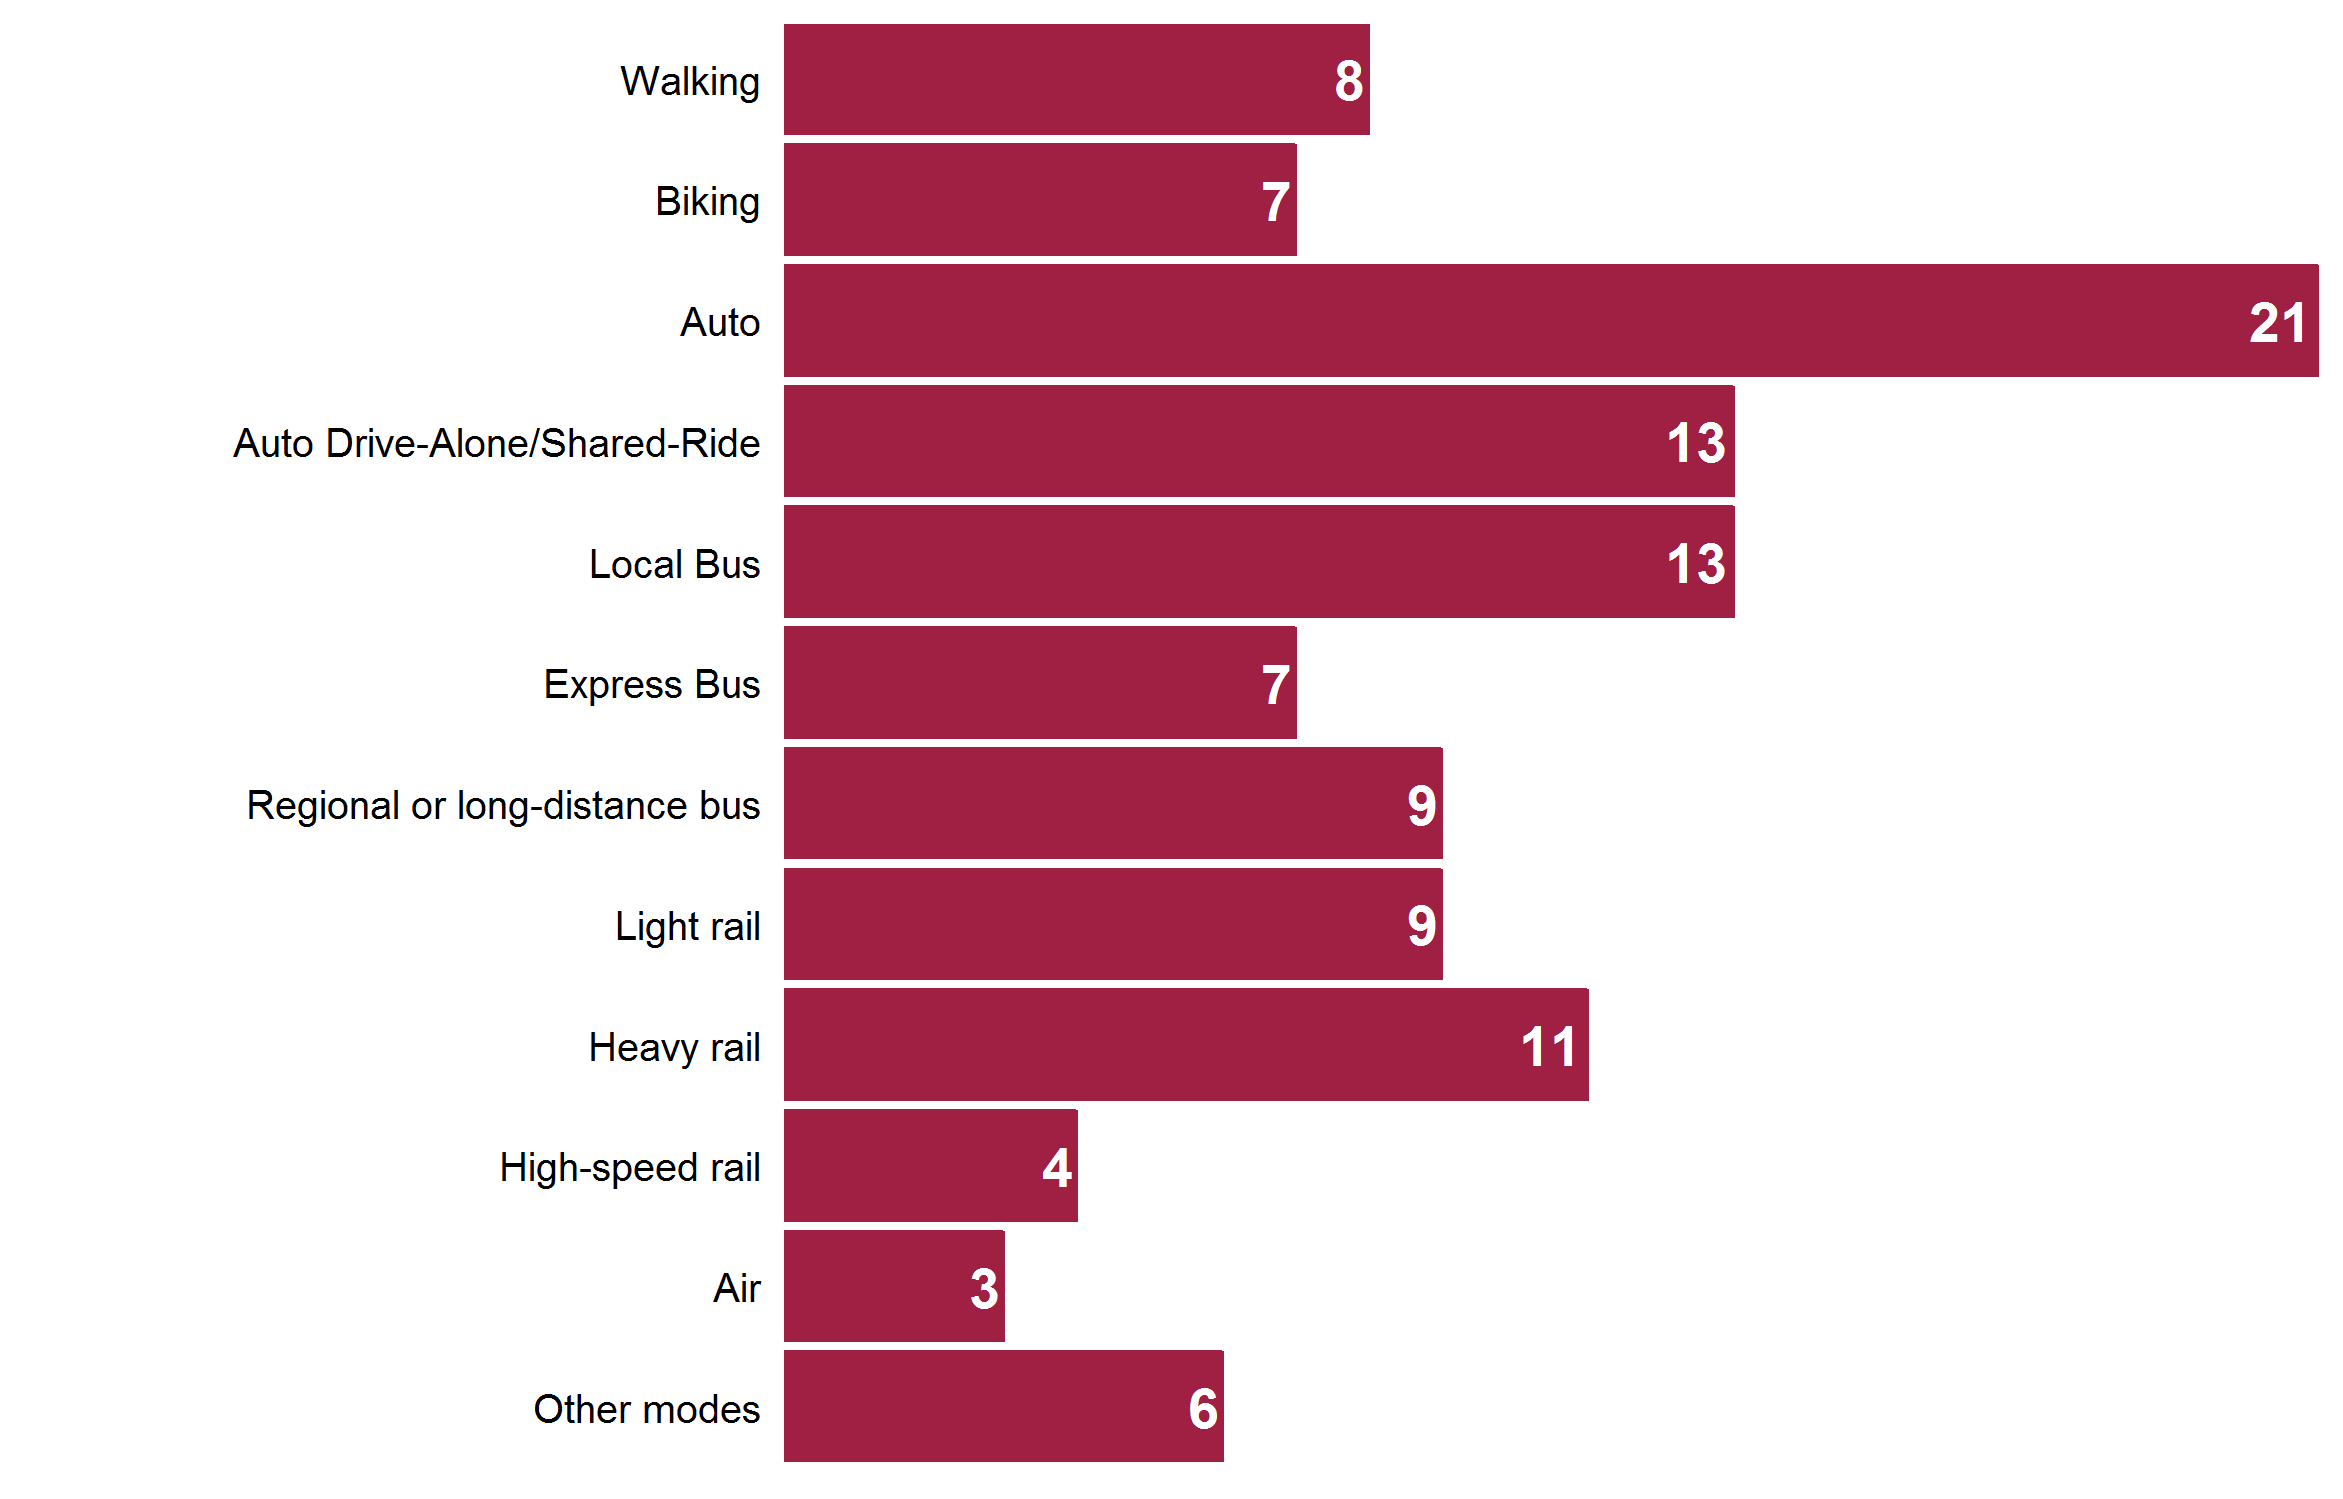
\includegraphics[width=6.4in]{graphics/10-person-modes-represented}
\caption[Modes represented in mode choice models for person travel]{Modes represented in mode choice models for person travel (multiple answers allowed)}
\label{fig:person-modes-represented}
\end{figure}

Eight models account for non-motorized travel as well. Often, the resolution in statewide models is too coarse to reasonably account for this mode. However, given the rising interest in non-motorized modes as an alternative to auto travel and for population health analyses, it is encouraging that almost a quarter of all statewide models account for them.

Local bus is the most frequently modeled transit mode, followed by heavy rail (which commonly includes commuter rail), regional or long-distance buses and light rail. High-speed rail is explicitly accounted for in the statewide models of California, Iowa, Maryland and Texas. Air travel is explicitly represented in the Florida, Oregon, and Texas models. However, the latter two have explicit long-distance models, where these modes most likely are handled.

The period of day that travel occurs within is represented in 12 out of 34 states (35 percent), as shown in Figure \ref{fig:time-of-day}. Note that this time-of-day separation applies to all traffic markets that are assigned to the highway network, including short and long-distance travel as well as person and freight trips. Congestion is found predominantly during peak hours, which is why many four-step models have added a fifth step to split the travel demand into a selected number of time-of-day periods. This way, congestion might be severe in the morning peak hours and cause travelers to switch to transit or choose detours to avoid bottlenecks, while during the mid-day period traffic could be comparatively light. Rural states with very low levels of congestion may omit this step, as travel time will not differ significantly by time of day.

\begin{figure}   % 11
\centering
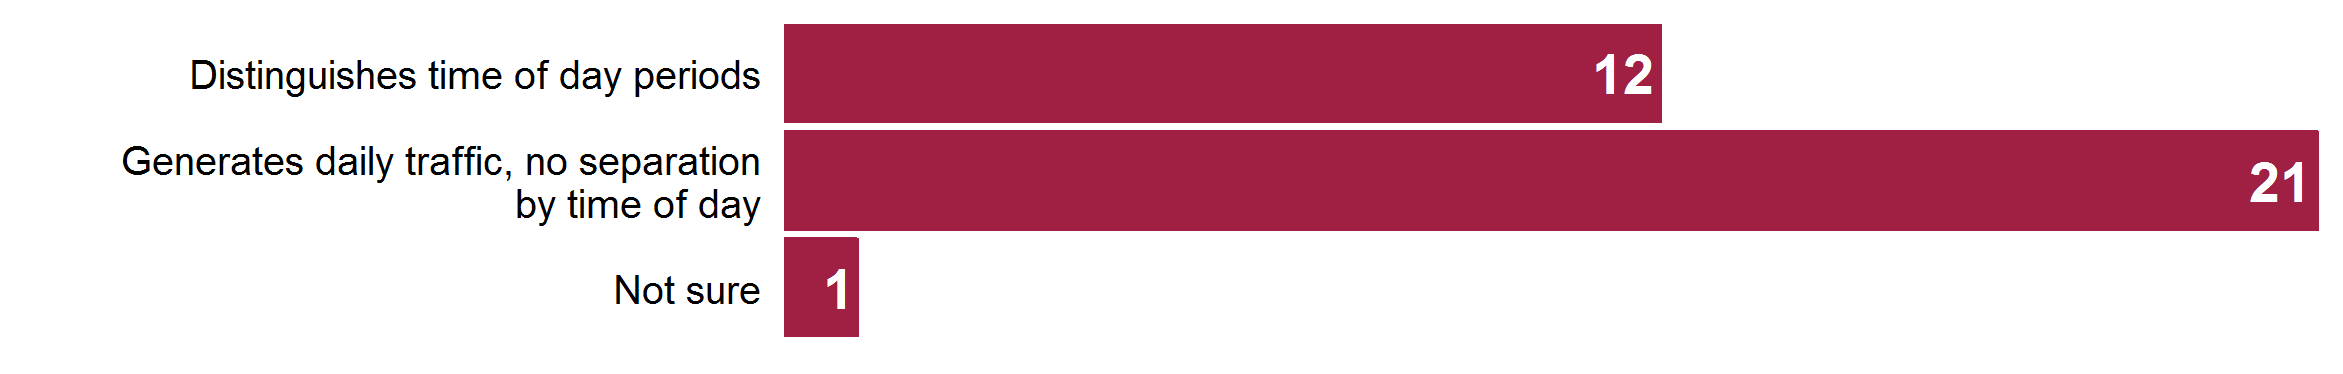
\includegraphics[width=6.4in]{graphics/11-time-of-day}
\caption{Time of day representation in statewide models}
\label{fig:time-of-day}
\end{figure}

The number of time-of-day periods distinguished by individual models is shown in Figure \ref{fig:time-periods-represented}. Most models deal with four time periods, usually defined as AM Peak, Midday, PM Peak and Night. Colorado is developing their model and intends to distinguish 7-10 periods. In general, a more fine-grained resolution of time is desirable. This will enable a model to represent better the time-dependent effects of congestion, which some travelers will attempt to avoid by traveling before or after those periods. However, more time intervals increase the computational burden and the need to model departure time shifts.

\begin{figure}[!bt]   % 12
\centering
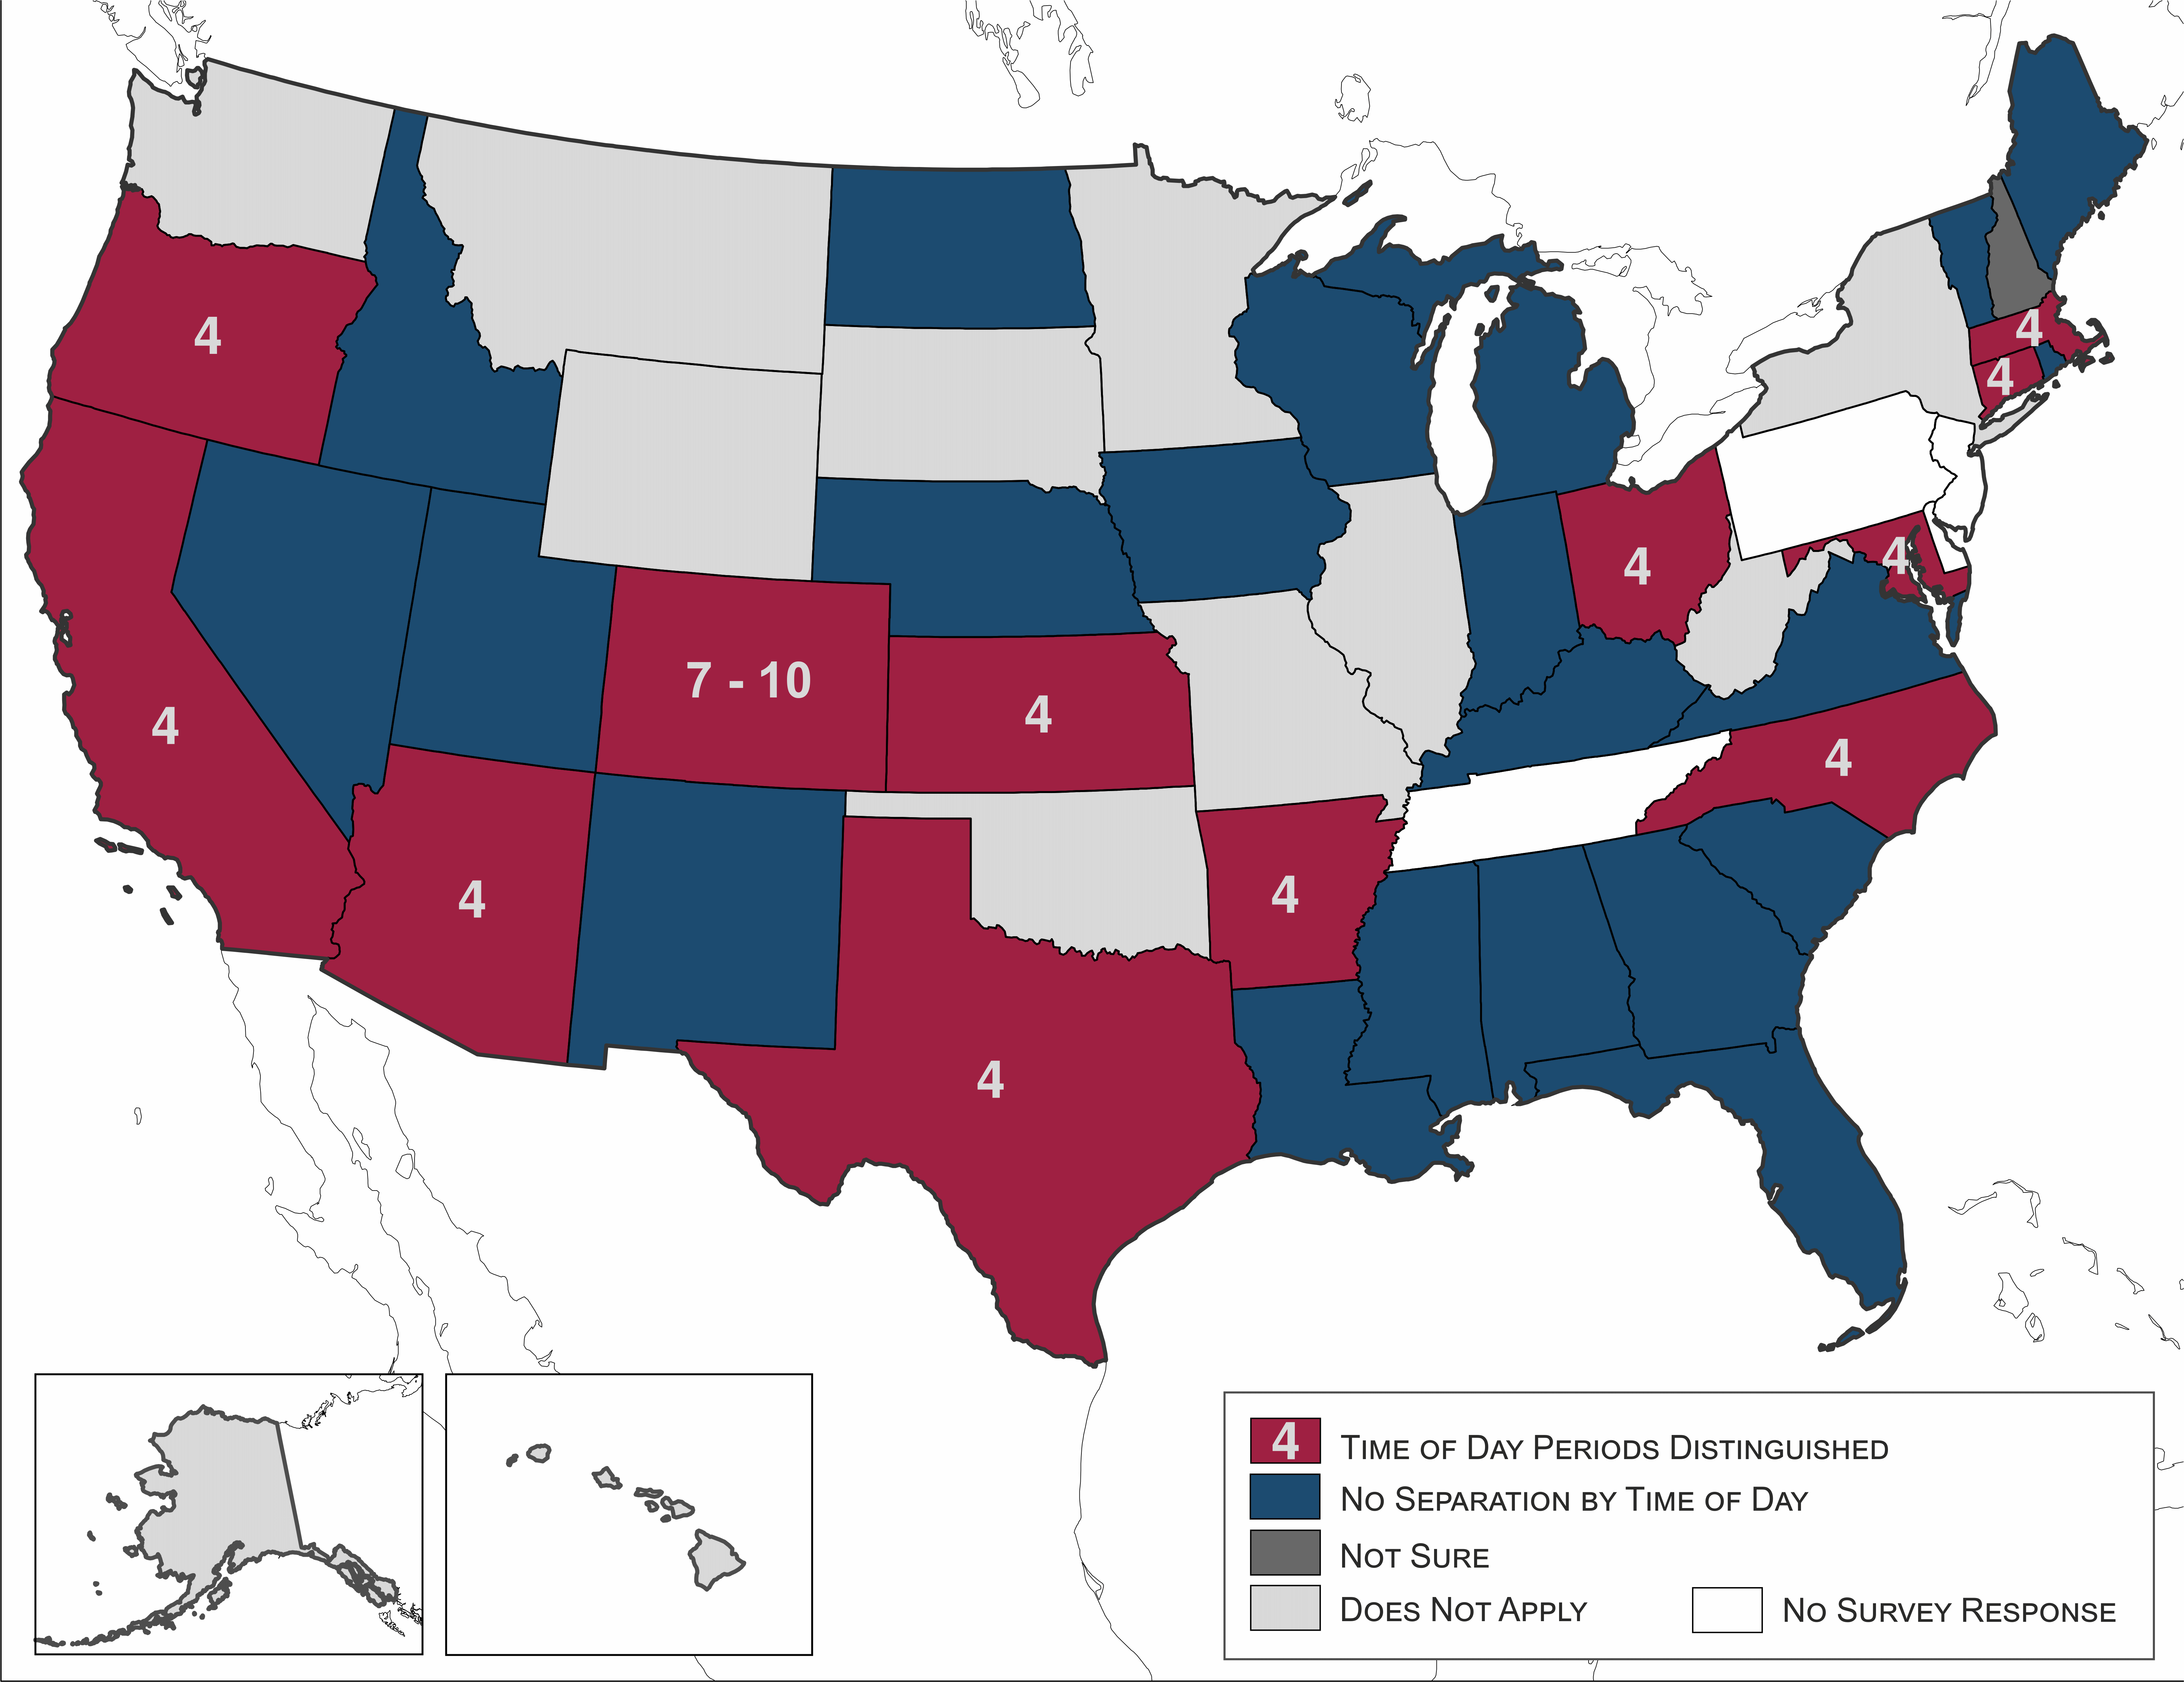
\includegraphics[width=6.5in]{graphics/12-time-periods-represented}
\caption{Number of time periods distinguished by individual statewide models}
\label{fig:time-periods-represented}
\end{figure}

Colorado, Ohio, and Oregon reported that their models generated travel demand in finer increments, representing 24 time-of-day periods in travel demand for Colorado and 19 for Ohio and Oregon. Due to runtime limitations, none of these models assigns all 24 or 19 time-or-day periods to the network (which was asked about in the responses shown in Figure \ref{fig:time-periods-represented}). However, those three models offer the ability to analyze travel demand in finer time intervals.

Four out of five statewide models use the traditional static user equilibrium algorithm for the assignment of highway travel, as shown in Figure \ref{fig:assignment-algorithms}. Alabama, Nebraska, and North Dakota apply the all-or-nothing assignment, presumably because intercity congestion in these states is very light and congested travel times does not differ much from free-flow travel times. Kansas uses a stochastic user equilibrium, and Maine applies an incremental capacity constraint model. Note that the assignment applies to all traffic markets that are assigned to the highway network, including short and long-distance travel as well as person and freight trips.

\begin{figure}   % 13
\centering
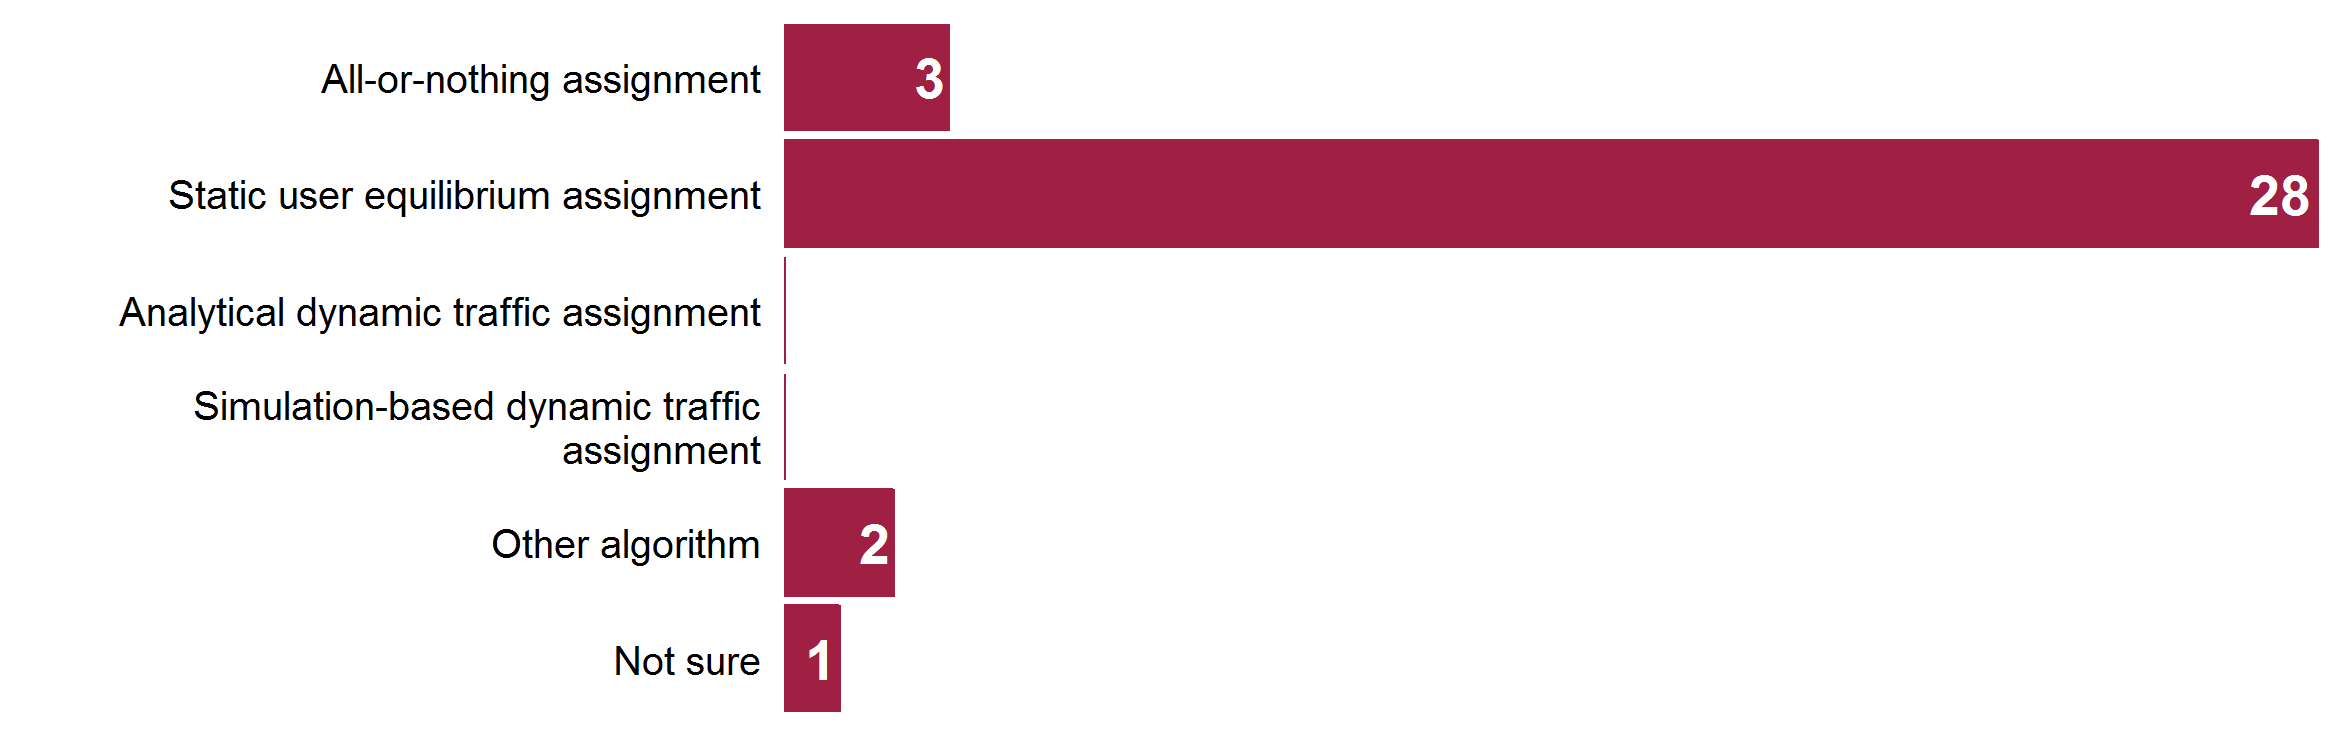
\includegraphics[width=6.4in]{graphics/13-assignment-algorithm}
\caption{Frequency of assignment algorithms in statewide models}
\label{fig:assignment-algorithms}
\end{figure}

Some models provide feedback from the assignment back to previous steps of the model. For example, under congested conditions some travelers may choose other destinations or other modes. By feeding back travel times to previous steps, an equilibrium between different submodules and congested travel times may be reached. The concept is shown for traditional four-step models in Figure \ref{fig:trip-based-feedback}. Feedback of congested travel times may also be provided for person long-distance travel and freight flows.

\begin{figure}   % 14
\centering
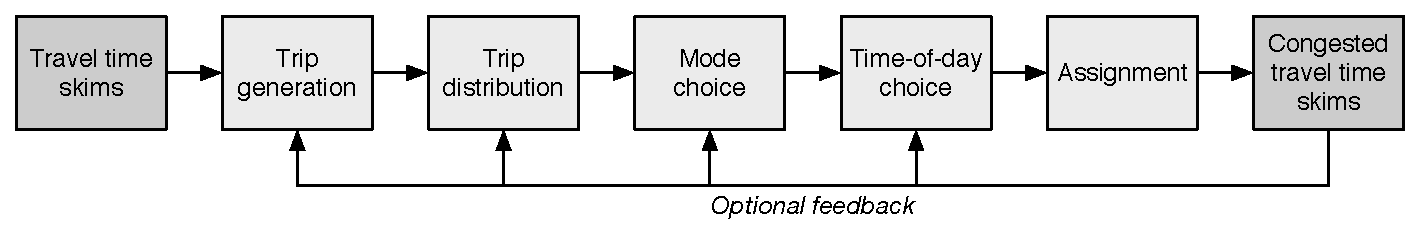
\includegraphics[width=6.4in]{graphics/14-feedback-process}
\caption{Trip-based model feedback process}
\label{fig:trip-based-feedback}
\end{figure}

Figure \ref{fig:feedback-frequency} shows how many statewide models apply feedback. Congested travel times are fed back into the trip distribution step in 20 out of 34 models (59 percent). As the mode choice model is run after the trip distribution model, presumably congested travel times affect mode choice in those models as well. Six models feed congested travel times back to trip generation.

\begin{figure}   % 15
\centering
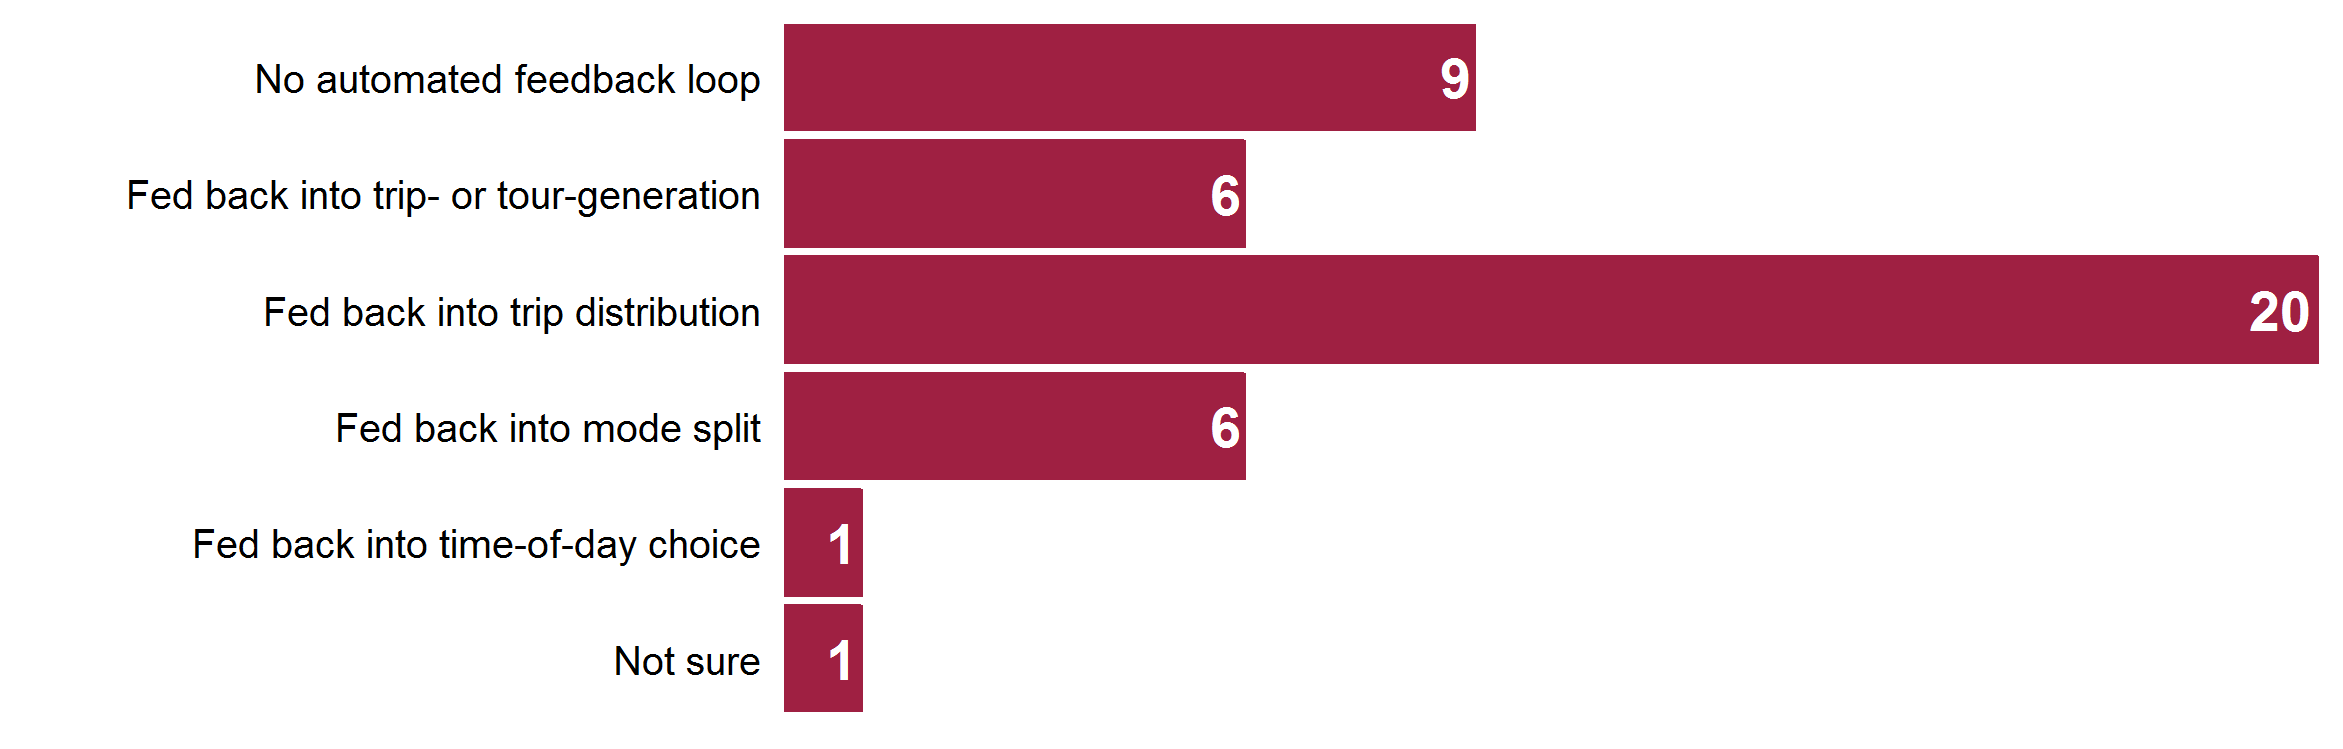
\includegraphics[width=6.4in]{graphics/15-feedback-frequency}
\caption[Frequency of feedback of congested travel times in statewide models]{Frequency of feedback of congested travel times in statewide models (multiple answers allowed)}
\label{fig:feedback-frequency}
\end{figure}

\section{Person long-distance travel}

Fifteen states (or 44 percent) have implemented explicit long-distance person travel demand models (Figure \ref{fig:person-long-distance-frequency}). No consistent definition of a long-distance trip exists, yet most states define long-distance travel as trips greater than 50 miles. This threshold is in line with the long-distance element of the 2001 NHTS survey. For Georgia, long-distance trips have been defined as 75 miles or more, for Nevada the threshold is 80 miles, and for Texas it is 150 miles. Arizona and North Carolina exclude long-distance commute trips (which are handled by the short-distance model because they are unlike most other habitual long-distance trips). For Alabama, long-distance trips are those that either cross the state boundary or travel across more than one MPO boundary, and for Colorado, trips that cross the state boundary are handled separately. Iowa is the only state that defines long-distance trips by travel time, namely greater than 60 minutes.

\begin{figure}   % 16
\centering

\includegraphics[width=6.4in]{graphics/16-person-long-distance-frequency}
\caption{Frequency of explicit long-distance models for person travel}
\label{fig:person-long-distance-frequency}
\end{figure}

Long-distance models tend to be implemented in larger states by area, as shown in Figure \ref{fig:person-long-distance-states}. However, some large states, such as California or Florida, do not operate long-distance models, while other smaller states, like Maryland, run long-distance models. Some states, such as Georgia, capture long-distance travel with a separate trip purpose in the short-distance travel model.

\begin{figure}   %  17
\centering
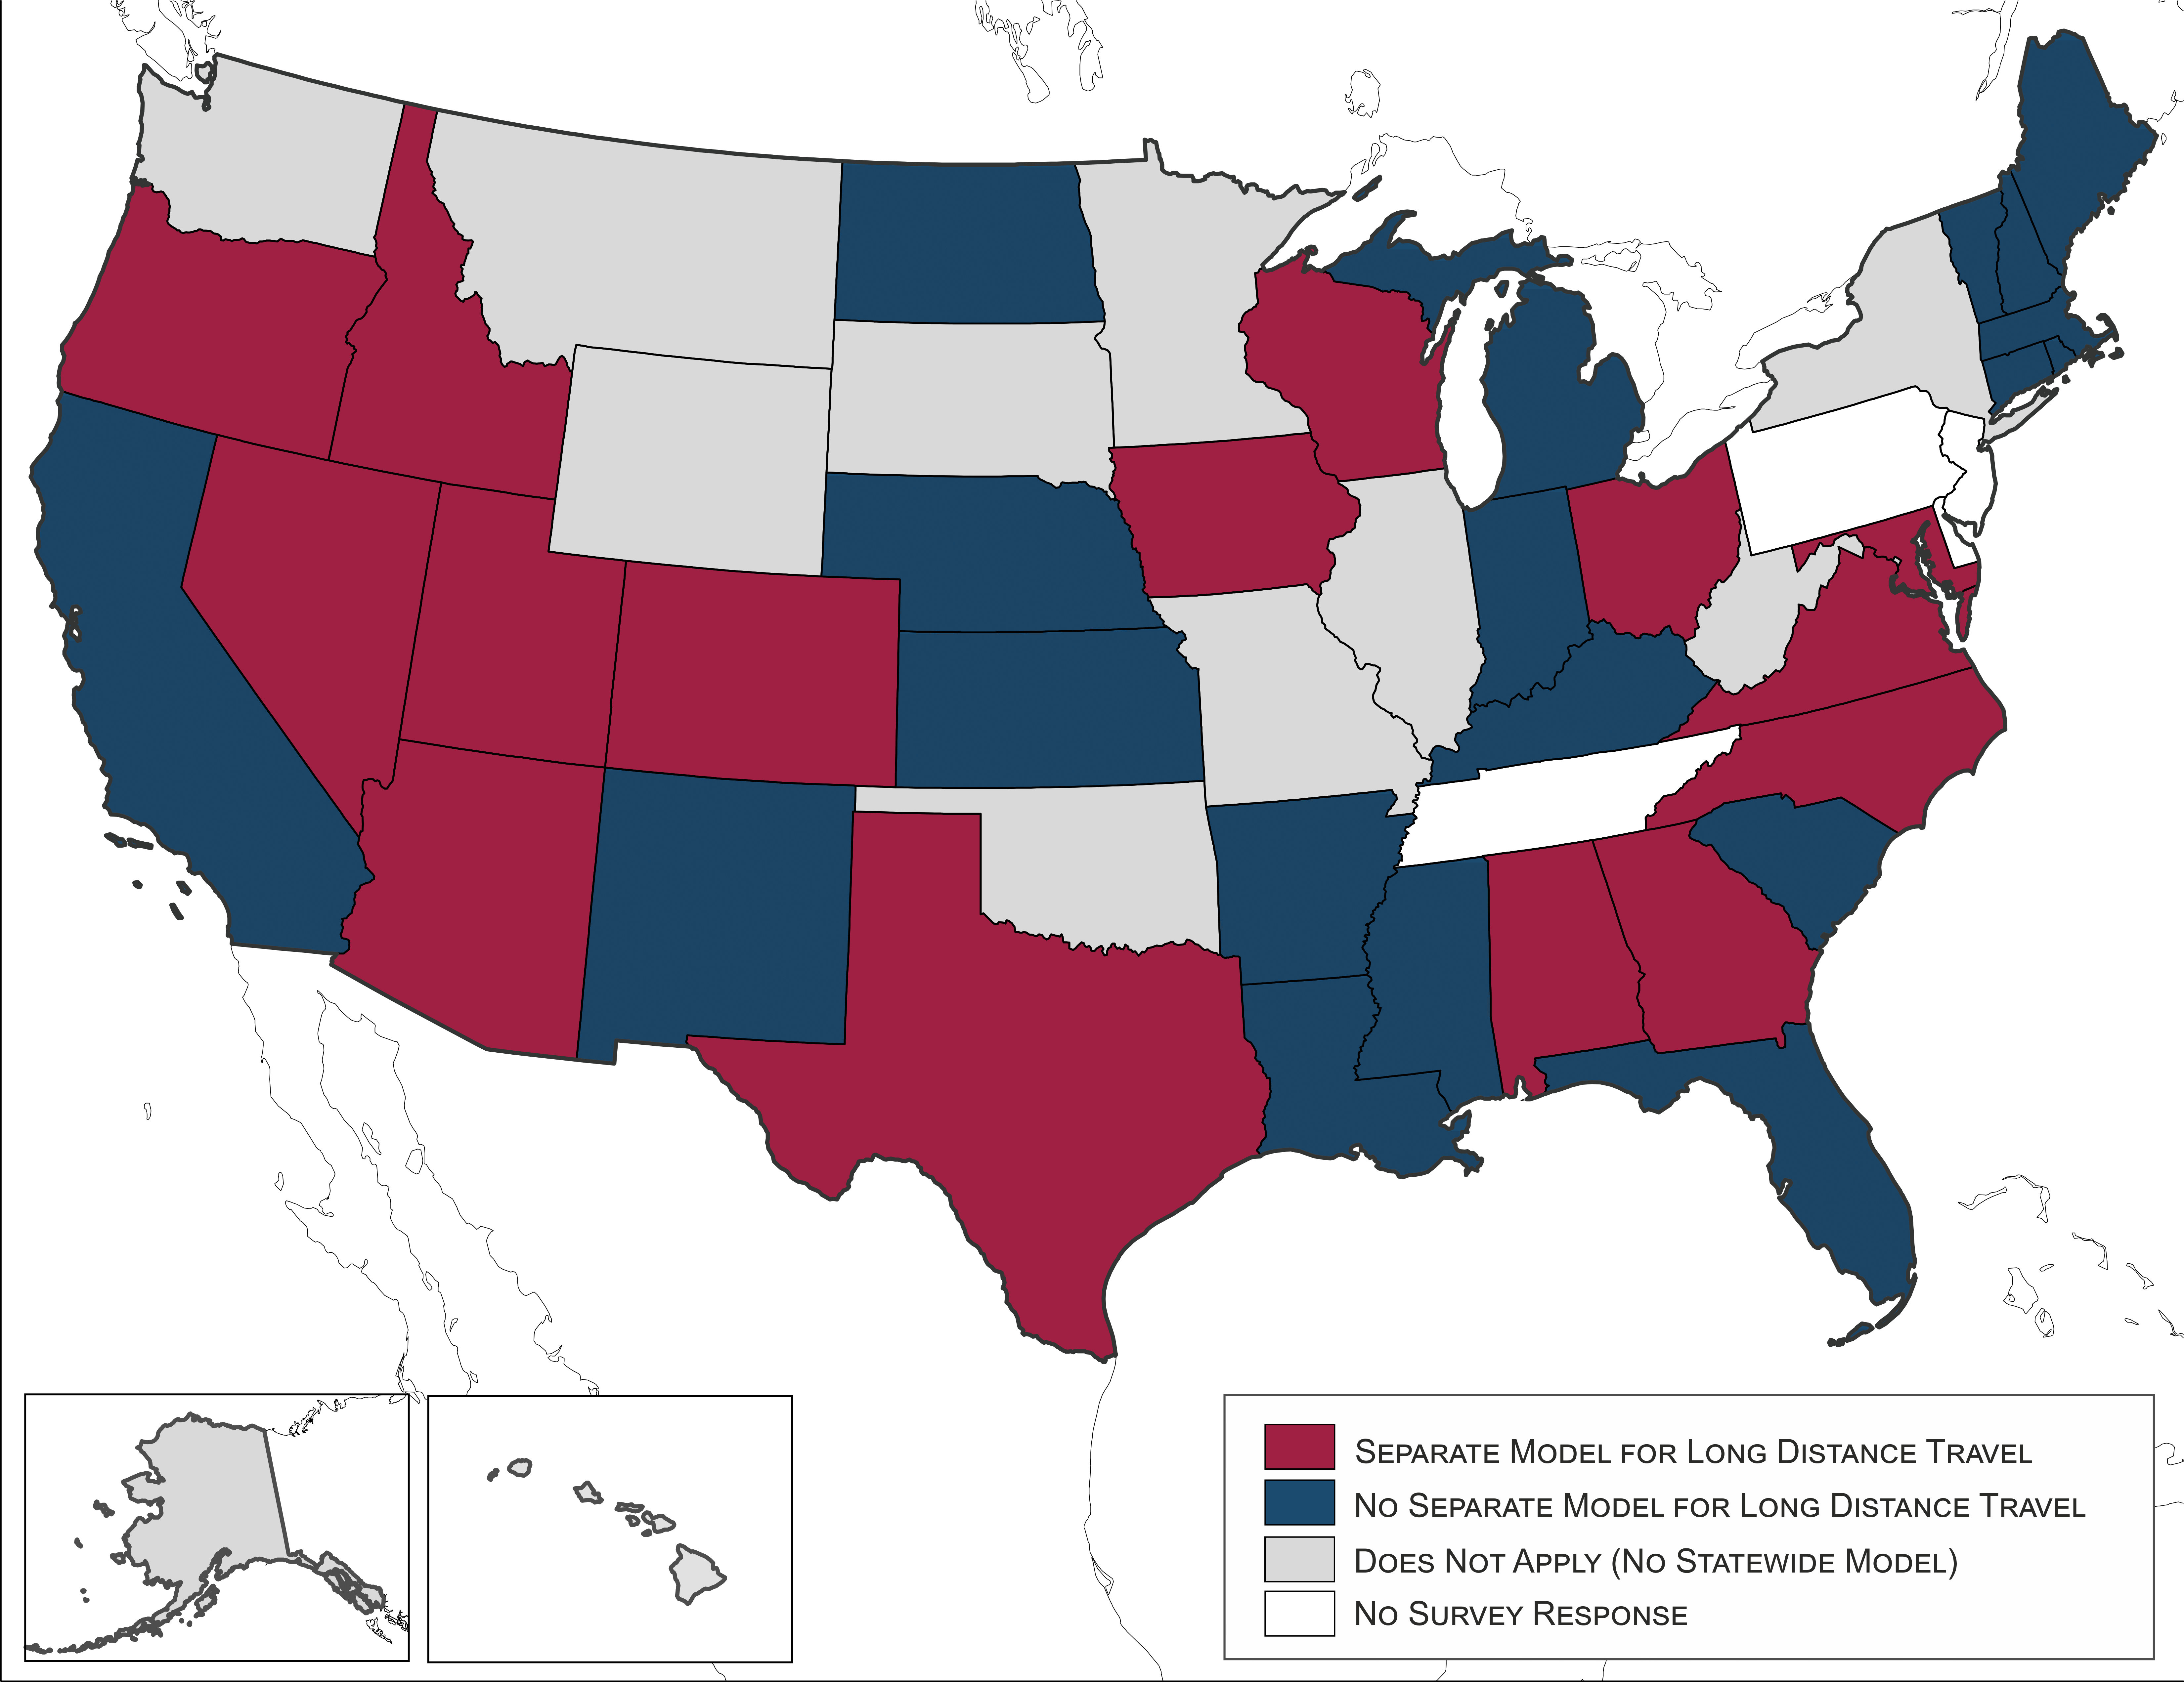
\includegraphics[width=6.4in]{graphics/17-person-long-distance-states}
\caption{States that operate separate long-distance models for person travel}
\label{fig:person-long-distance-states}
\end{figure}

A wide variety of sources are used for trip generation of long-distance trips, as summarized in Figure \ref{fig:person-long-distance-generation}. Iowa is currently the only state that uses FHWA's national long-distance person model \citep{outwater14, outwater15} and trip rates provided in NCHRP Report 735 \citep{schiffer12}. Arizona, Maryland, and North Carolina use the long-distance model NELDT \citep{moeckel11}, which is based on trip frequencies reported in the long-distance element of the 2001 NHTS.

\begin{figure}   % 18
\centering
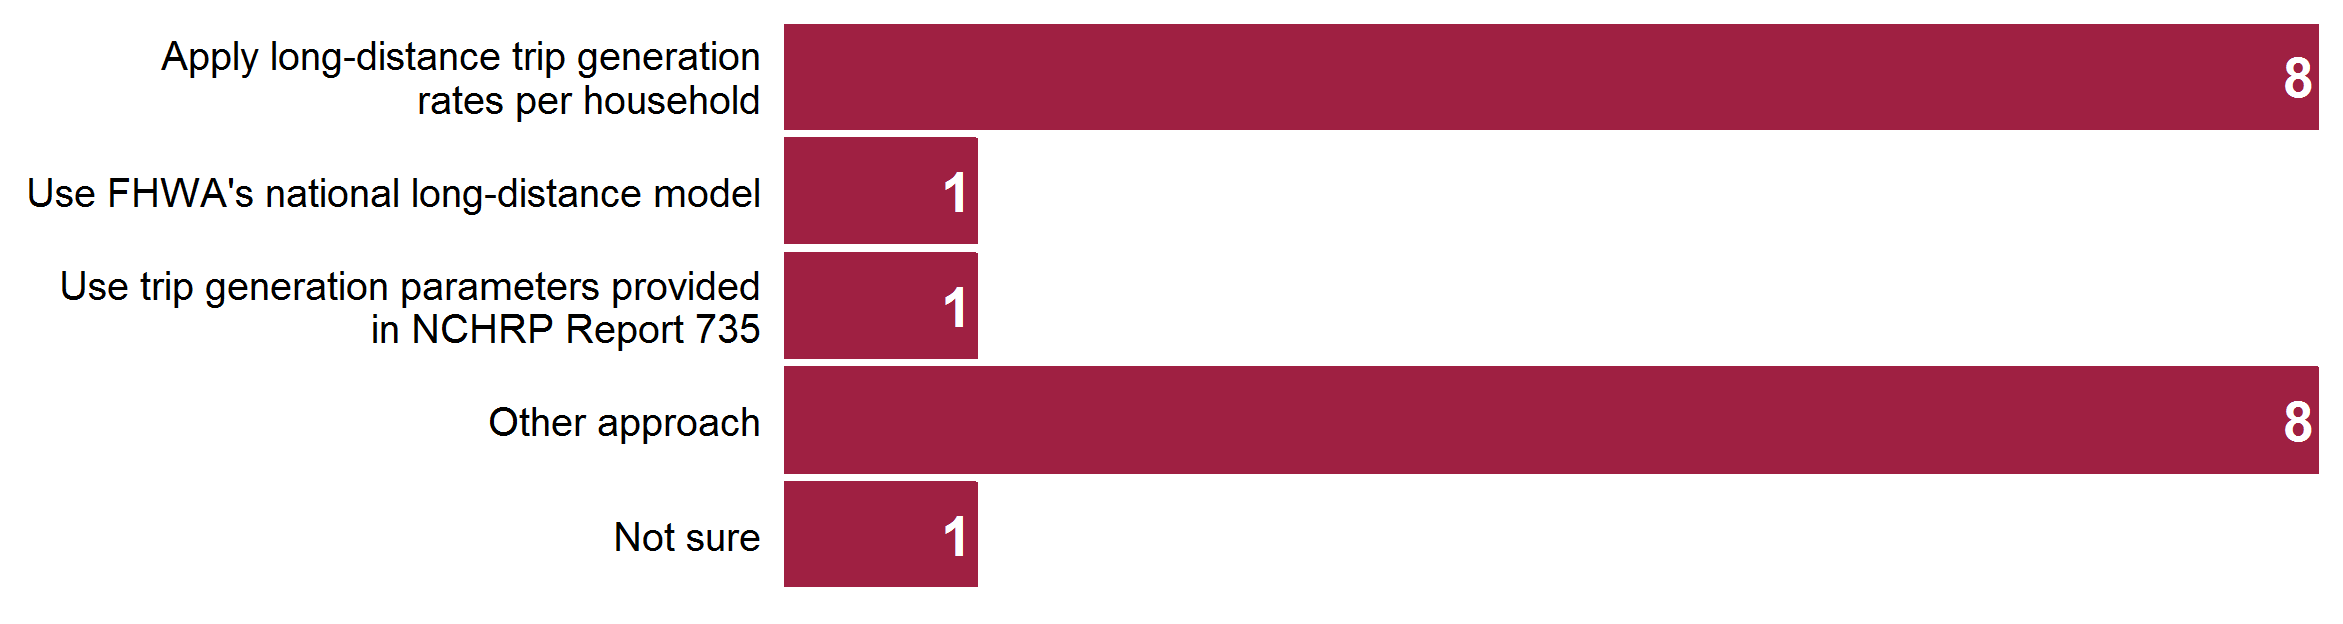
\includegraphics[width=6.4in]{graphics/18-person-long-distance-generation}
\caption[Travel demand generation rates for person long-distance travel]{Travel demand generation rates for person long-distance travel (multiple answers allowed)}
\label{fig:person-long-distance-generation}
\end{figure}

Most long-distance models use traditional gravity models for trip distribution, as shown in Figure \ref{fig:person-long-distance-distribution}. The shortcomings of this approach have already been discussed in \S\ref{sec:person-demand-modeling}, though using separate gravity models for short- and long-distance travel makes that criticism less severe. Five states use advanced logit-based destination choice models, making the one-third share of this approach similar to the pattern found for short-distance travel models.

\begin{figure}   % 19
\centering
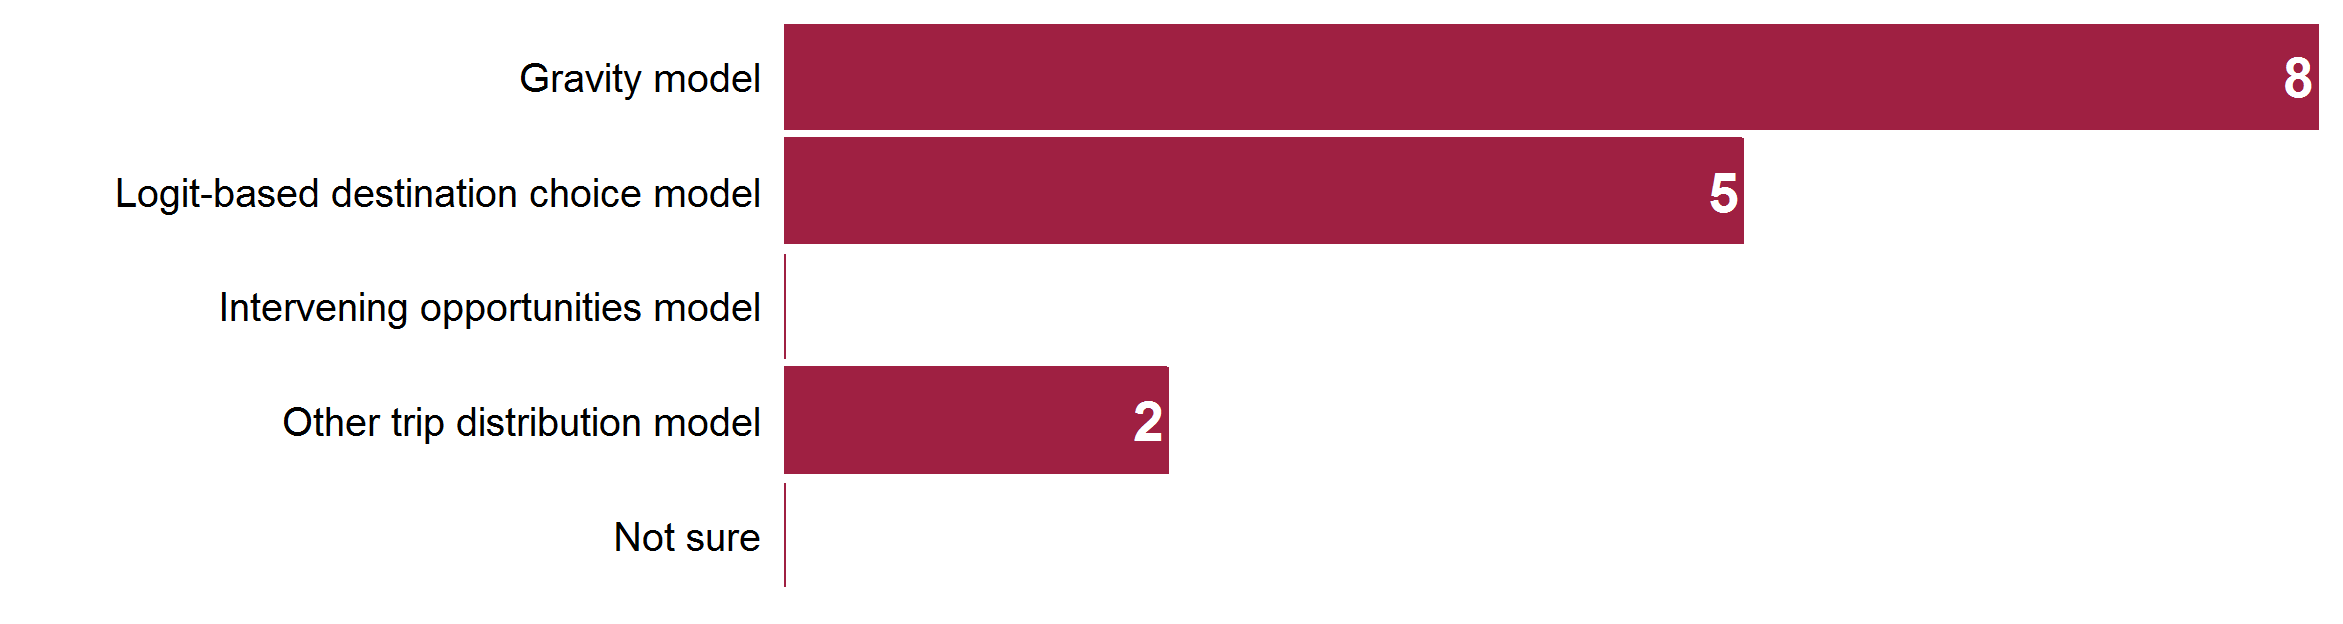
\includegraphics[width=6.4in]{graphics/19-person-long-distance-distribution}
\caption{Frequency of trip distribution models for long-distance person travel}
\label{fig:person-long-distance-distribution}
\end{figure}

About half of all long-distance models apply nested multinomial mode choice models (Figure \ref{fig:person-long-distance-mode-choice}). Wisconsin uses a multinomial model, and Utah applies static mode shares (consistent with their short-distance mode choice model). Colorado selected other mode choice model, as all intra-state trips are handled by the short-distance mode choice model; no mode choice model is planned at this time for interstate trips. Alabama, Arizona, Maryland and Nevada generate long-distance trips for autos only.

\begin{figure}   % 20
\centering
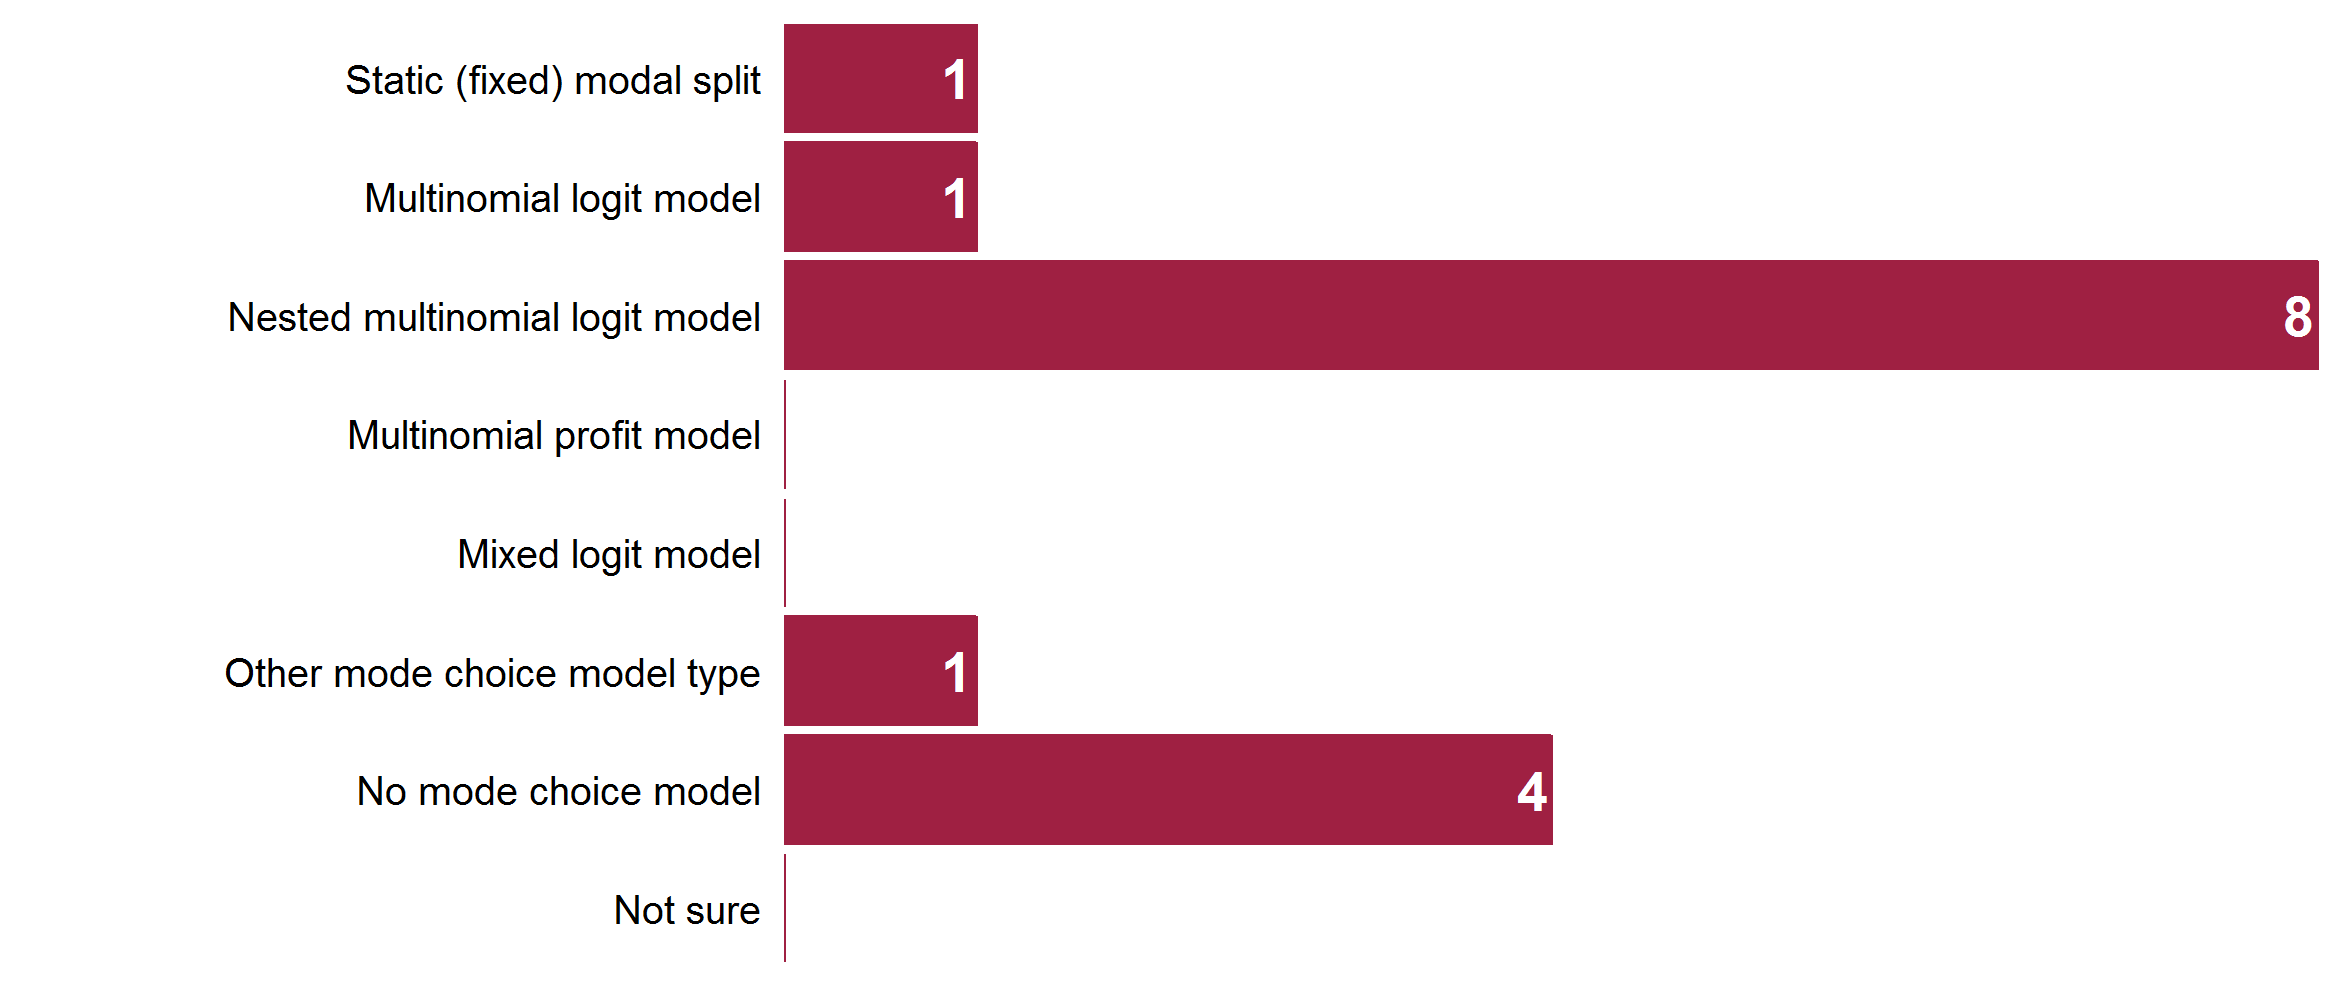
\includegraphics[width=6.4in]{graphics/20-person-long-distance-mode-choice}
\caption{Frequency of mode choice models for long-distance travel}
\label{fig:person-long-distance-mode-choice}
\end{figure}

The modes of transportation represented by long-distance travel models are shown in Figure \ref{fig:person-long-distance-modes}. Obviously, non-motorized travel is not modeled for long-distance travel. All states model the auto mode, and five models distinguish drive-alone from shared-ride. Many include bus, rail, and air, with Georgia, Maryland, Oregon and Texas offering the option to represent high-speed rail explicitly. California has developed a separate high-speed rail model that is not integrated with the statewide model, as described in \S\ref{sec:california-hsr-model} (page \pageref{sec:california-hsr-model}).

\begin{figure}   % 21
\centering
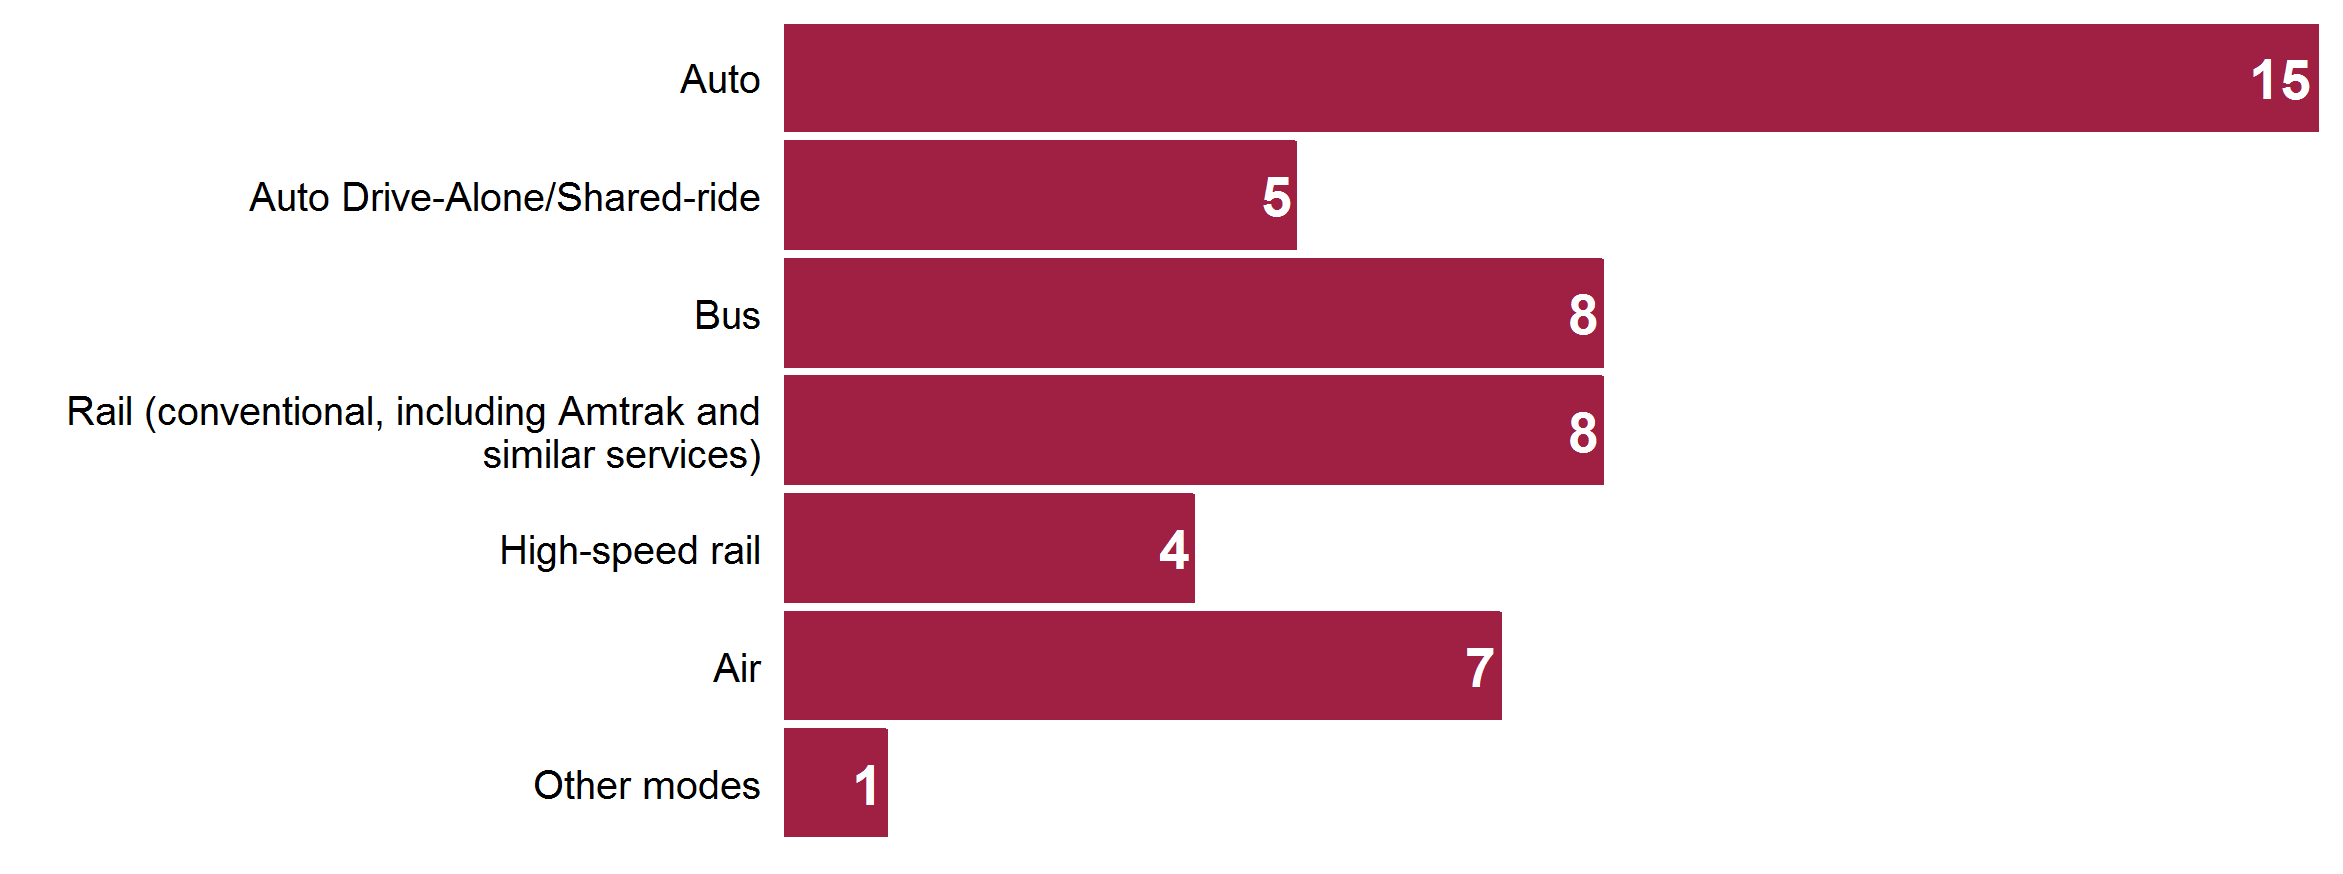
\includegraphics[width=6.4in]{graphics/21-person-long-distance-modes}
\caption[Modes represented in long-distance person mode choice models]{Modes represented in long-distance person mode choice models (multiple answers allowed)}
\label{fig:person-long-distance-modes}
\end{figure}

\section{ Freight models}

Travel demand modeling has traditionally focused on person travel by auto. This is not surprising, as autos generate over 90 percent of all vehicle-miles traveled \citep{fhwa16b}, while trucks make up only 4.1 percent of all registered vehicles and only 2.5 percent of all new vehicle sales in the United States \citep{bea16}. However, trucks generate the core demand for transportation infrastructure maintenance. For example, the rear axles of a typical 13-ton van cause 1,000-times the structural damage of a car (\cite{small89}:11). Ketcham estimated that 95 percent of all highway damage is caused by heavy trucks (\cite{mackenzie92}:9). Trucks also consume 25 percent of all fuel in the United States \citep{bts16}, contributing disproportionately to greenhouse gas emissions. Furthermore, growth in freight transportation is expected to significantly outpace growth in passenger transportation (\cite{chow10}:1012). Moreover, easing freight travel has become a mantra for economic development \citep{mckinnon06}. The ratio between freight-miles traveled and the Gross Domestic Product, also known as the freight-transportation intensity, shows a strong (yet gradually declining) relationship between freight activity and economic growth.

Given their disproportional impact upon the transportation system, it is not surprising that most statewide models account for freight modeling (Figure \ref{fig:freight-models-frequency}), particularly in areas with high levels of congestion. As freight tends to make up a higher share of traffic on rural roads, statewide models tend to have a larger share of freight traffic than urban models. Therefore, statewide models tend to pay more attention to freight flows, often distinguishing short- and long-distance freight flows. While short-distance trucks are covered by 21 states (62 percent of all states with statewide models), long-distance trucks are modeled by 26 states (76 percent). Connecticut uses static truck trips tables, and Nebraska plans to add them within the next year. Doing so enables these states to at least account for truck volumes on the network, even though truck flows would not be scenario sensitive.

\begin{figure}   % 22
\centering
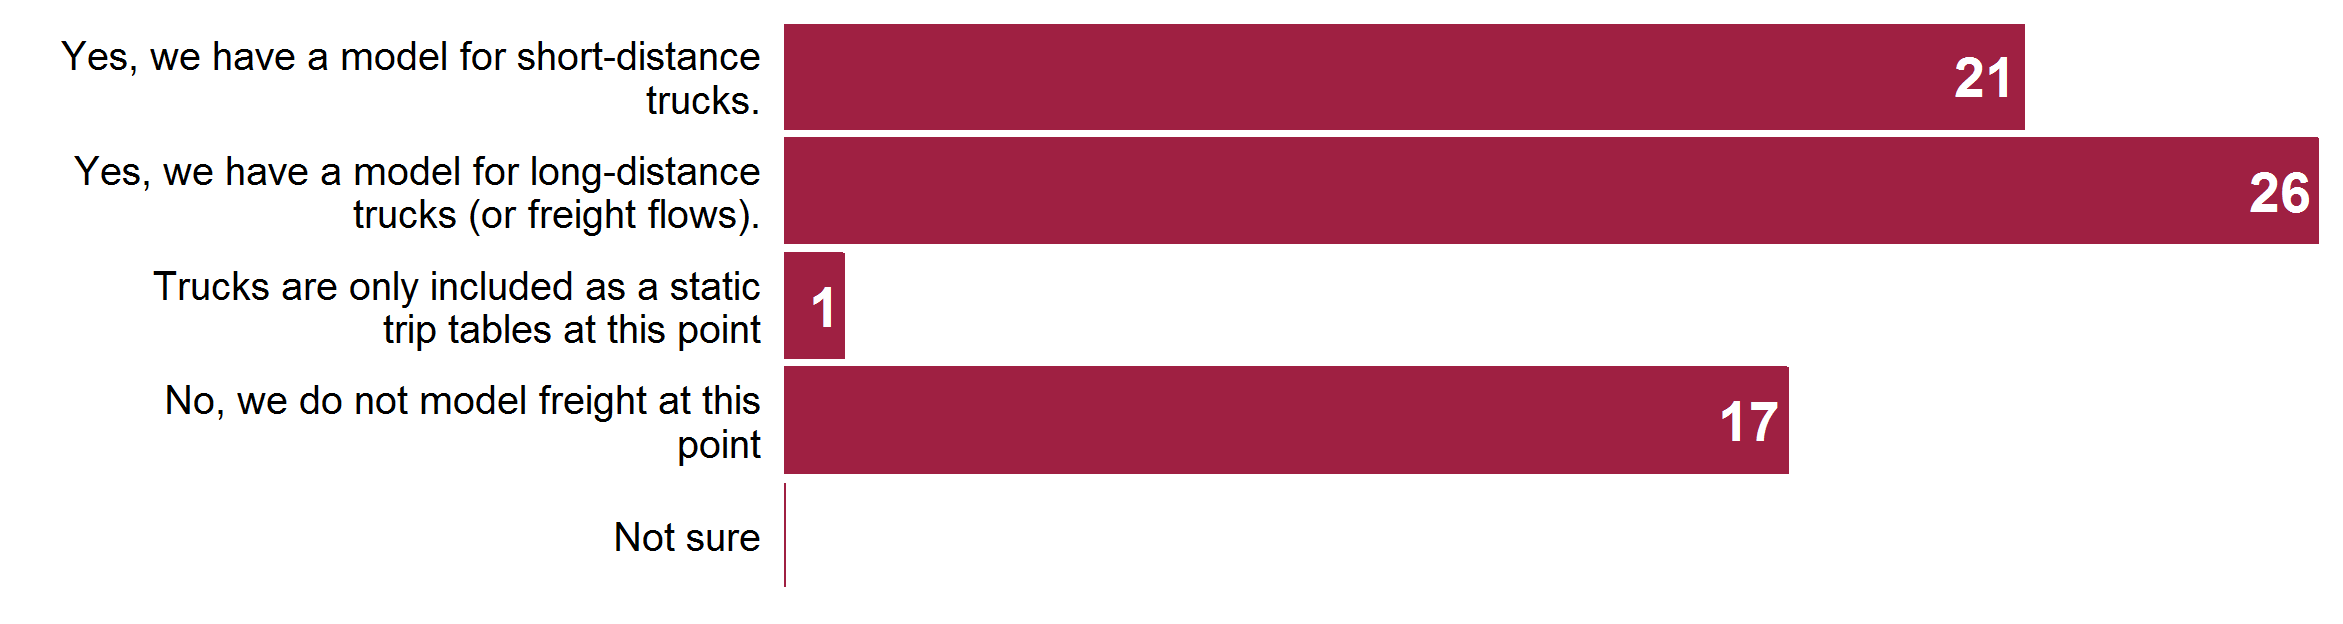
\includegraphics[width=6.4in]{graphics/22-freight-models-frequency}
\caption{Frequency of freight models in statewide models}
\label{fig:freight-models-frequency}
\end{figure}

Of the 21 states that model short-distance trucks, 19 use trip-based models, and only Ohio and Oregon use tour-based truck models. The limitations of trip-based truck models have been discussed extensively in the literature \citep{holguinveras13}, yet it is no surprise that tour-based models are uncommon in statewide models. The heterogeneous travel behavior of trucks (depending, among other factors, on truck type and commodities carried) and the limited freight data availability (much more so than for auto travel) make it inherently challenging to represent tour-based travel behavior for trucks. However, a few operational tour-based models in addition to Ohio and Oregon have been implemented for Alberta \citep{hunt07}, Guatemala City \citep{holguinveras03}, Rome \citep{nuzzolo13} and the San Pedro Bay Ports in Southern California \citep{you12}. Given the increasing interest in freight in many states, it is expected that more will follow the examples of Ohio and Oregon in tour-based truck modeling in the future.

The spatial distribution of long-distance freight models is shown in Figure \ref{fig:freight-long-distance-states}. Clusters of them are apparent in the Southwest, the South, and the Great Lakes area. Freight modeling appears to be less common in states in the northern parts of the U.S. The Interstate 10 corridor and possibly the I-65 corridor (though Tennessee did not participate in this survey) are the only ones that are covered completely by statewide truck models. Several states in the Midwest and New England have not tackled freight flow models yet. Given the especially large volumes of long-distance truck flows on east-west highway corridors, many states might benefit from explicitly modeling them.

\begin{figure}   % 23
\centering
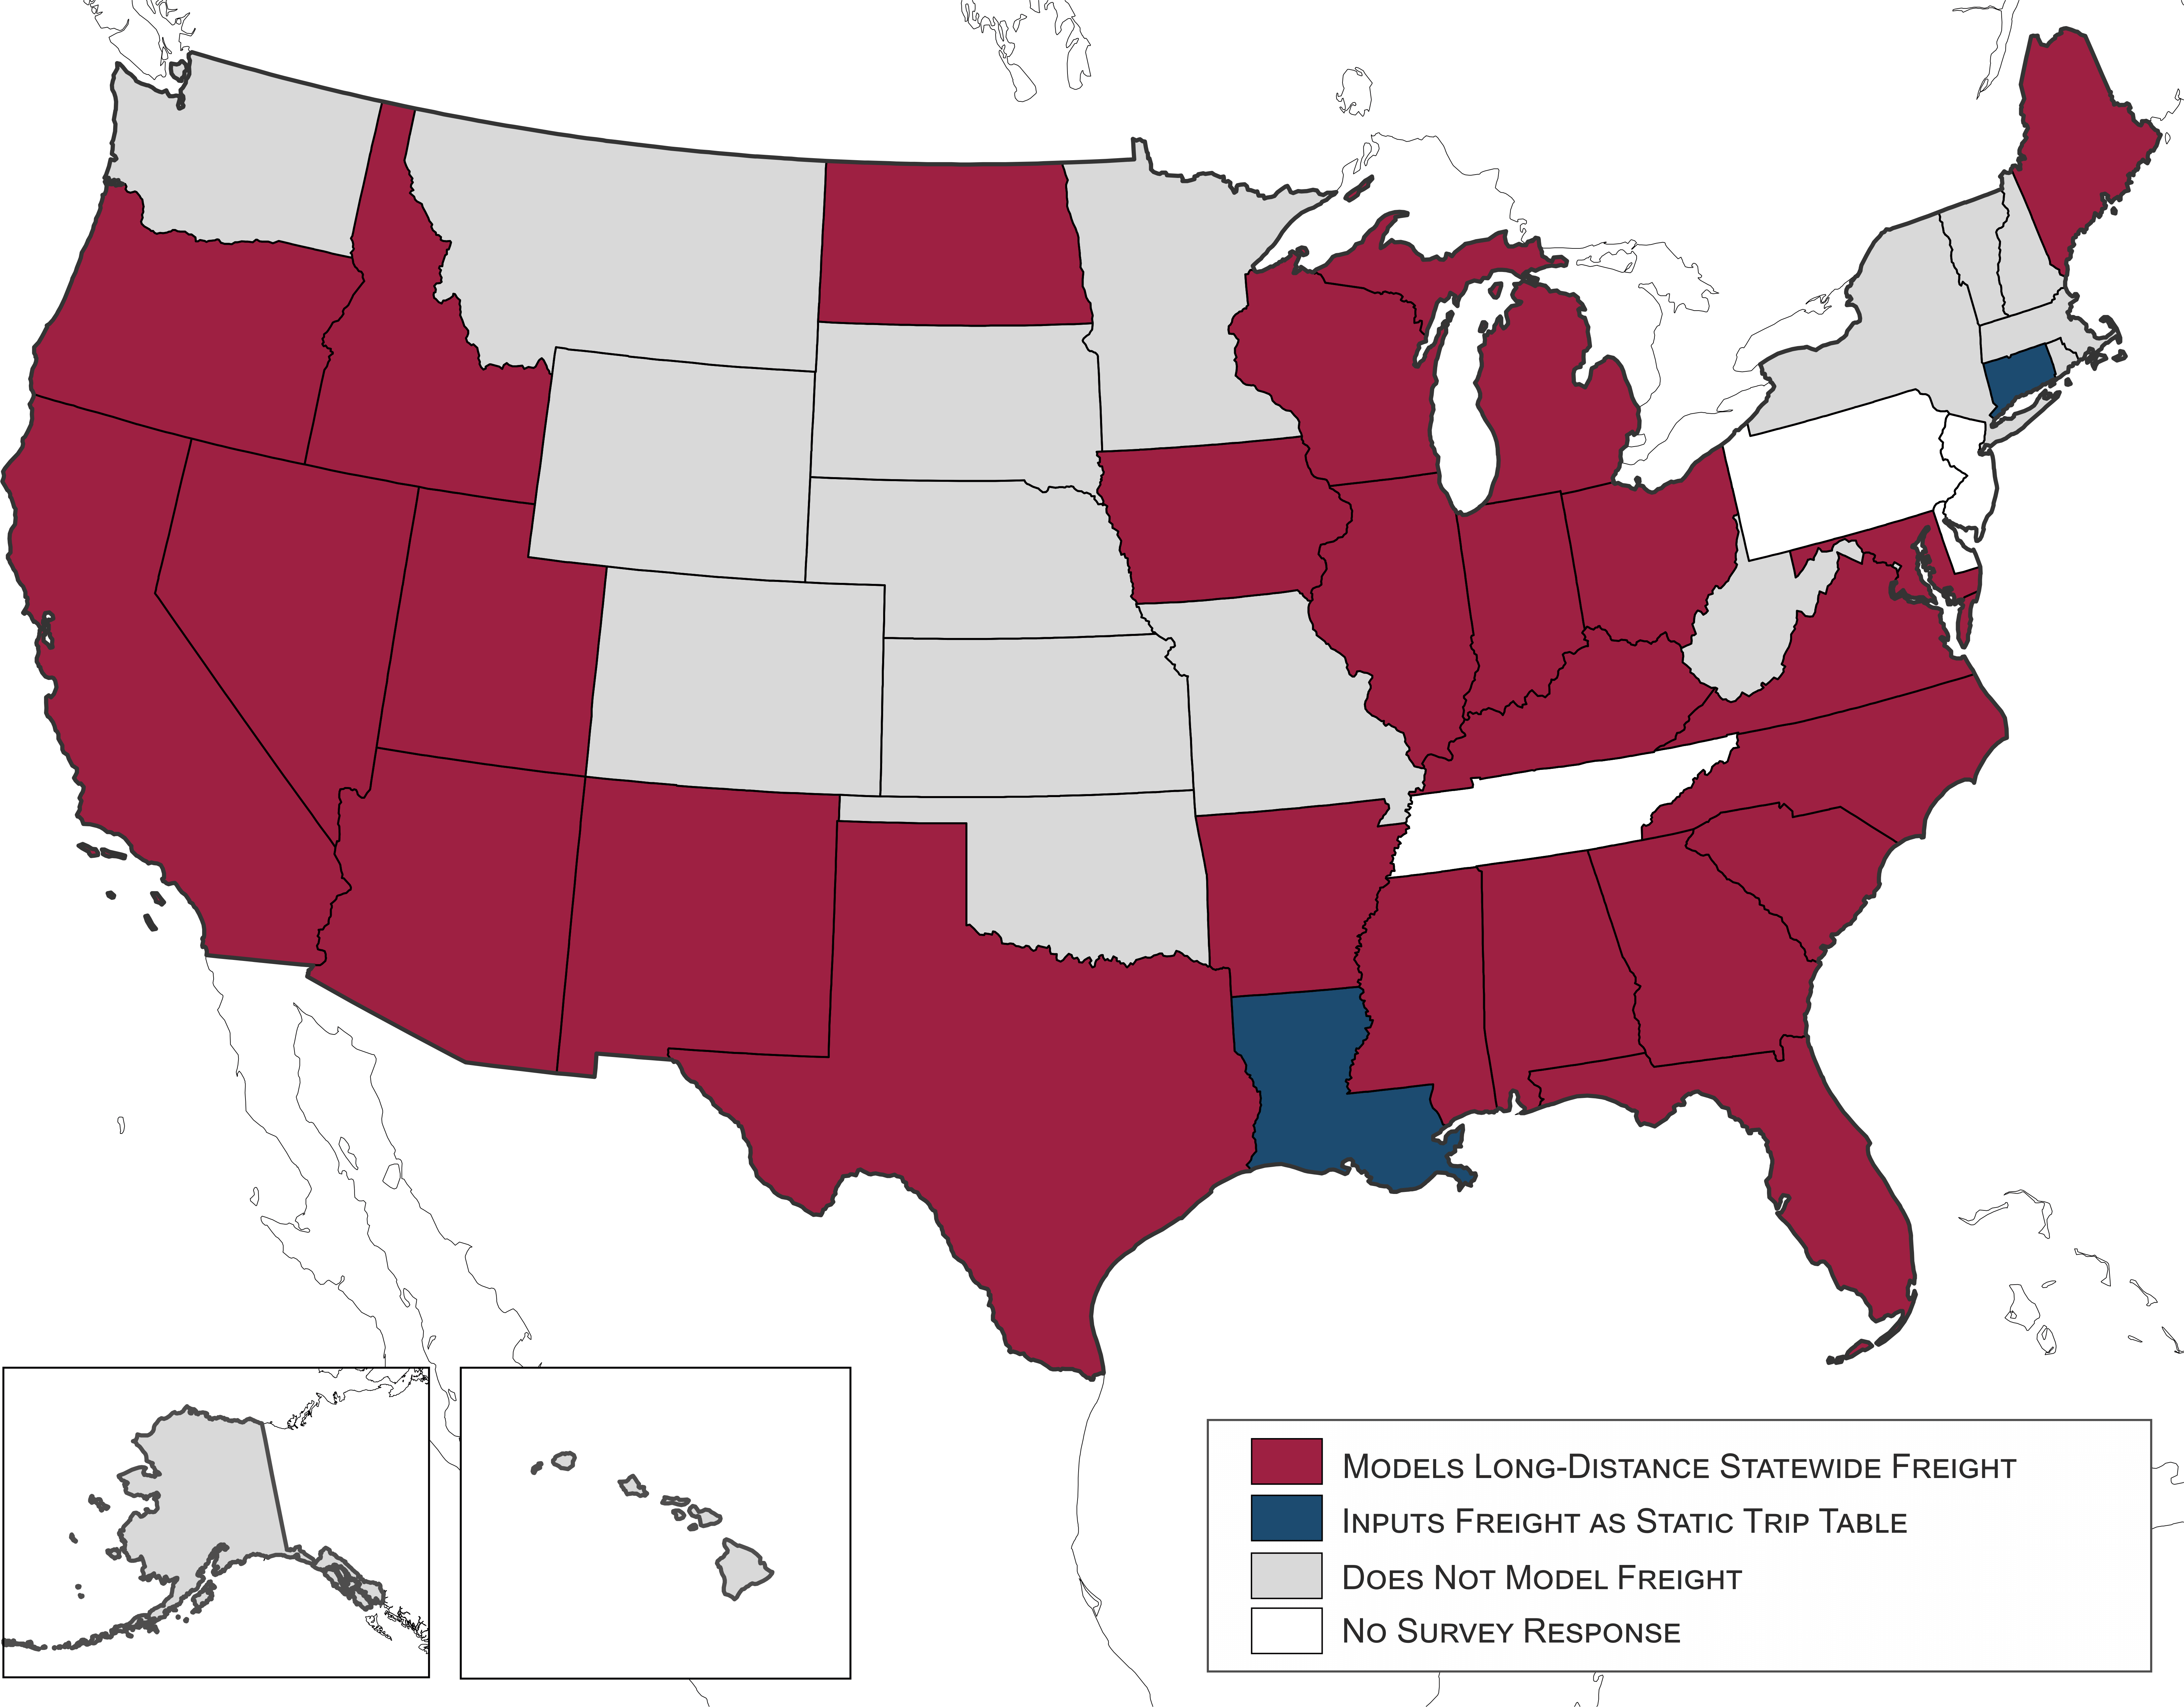
\includegraphics[width=6.5in]{graphics/23-freight-long-distance-states}
\caption{States operating long-distance freight models}
\label{fig:freight-long-distance-states}
\end{figure}

Long-distance truck modeling is dominated by commodity flow models (Figure \ref{fig:freight-long-distance-methods}). Illinois uses a supply chain model, though publicly available data for such modeling approach is very limited. Most of the respondents who reported using commodity flow models in the survey reported that they are based, at least in part, upon origin-destination freight flow data from the Freight Analysis Framework (FAF), as described in \S\ref{sec:traditional-freight-data} (page \pageref{sec:traditional-freight-data}). Presumably, many of these models are not policy-sensitive commodity flow models, but rather static transformations of exogenous FAF commodity flows converted into truck flows. Nine states use FAF payload factors to convert freight flows in tons into truckload equivalents.

\begin{figure}   % 24
\centering
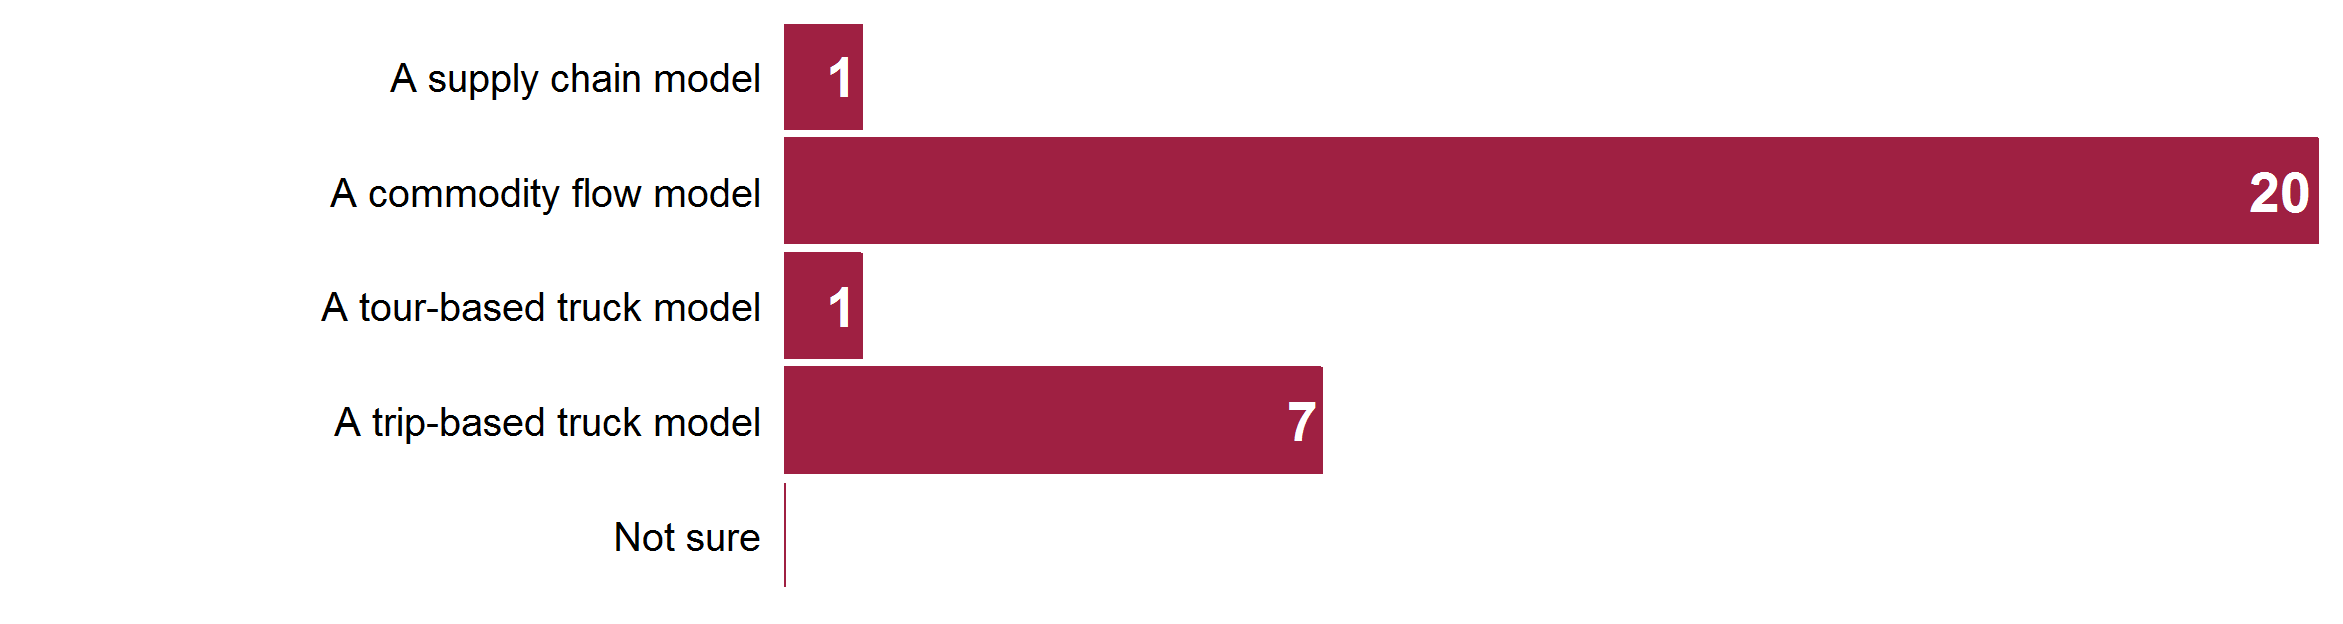
\includegraphics[width=6.4in]{graphics/24-freight-long-distance-methods}
\caption[Frequency of long-distance freight modeling methods]{Frequency of long-distance freight modeling methods (multiple answers allowed)}
\label{fig:freight-long-distance-methods}
\end{figure}

A growing number of states apply mode choice models to freight flows as well (Figure \ref{fig:freight-mode-choice}). Out of 26 states that model long-distance freight flows, six states (23 percent) apply rule-based freight mode choice models. Such models do not attempt to econometrically estimate mode shares, but rather apply simple rules of modal allocation that can be reviewed and changed. For example, rules may include that short-distance flows rarely use rail or water modes, only high-value goods move by air, and vessels can only be used if there is a waterway on at least part of the trip.

\begin{figure}   % 25
\centering
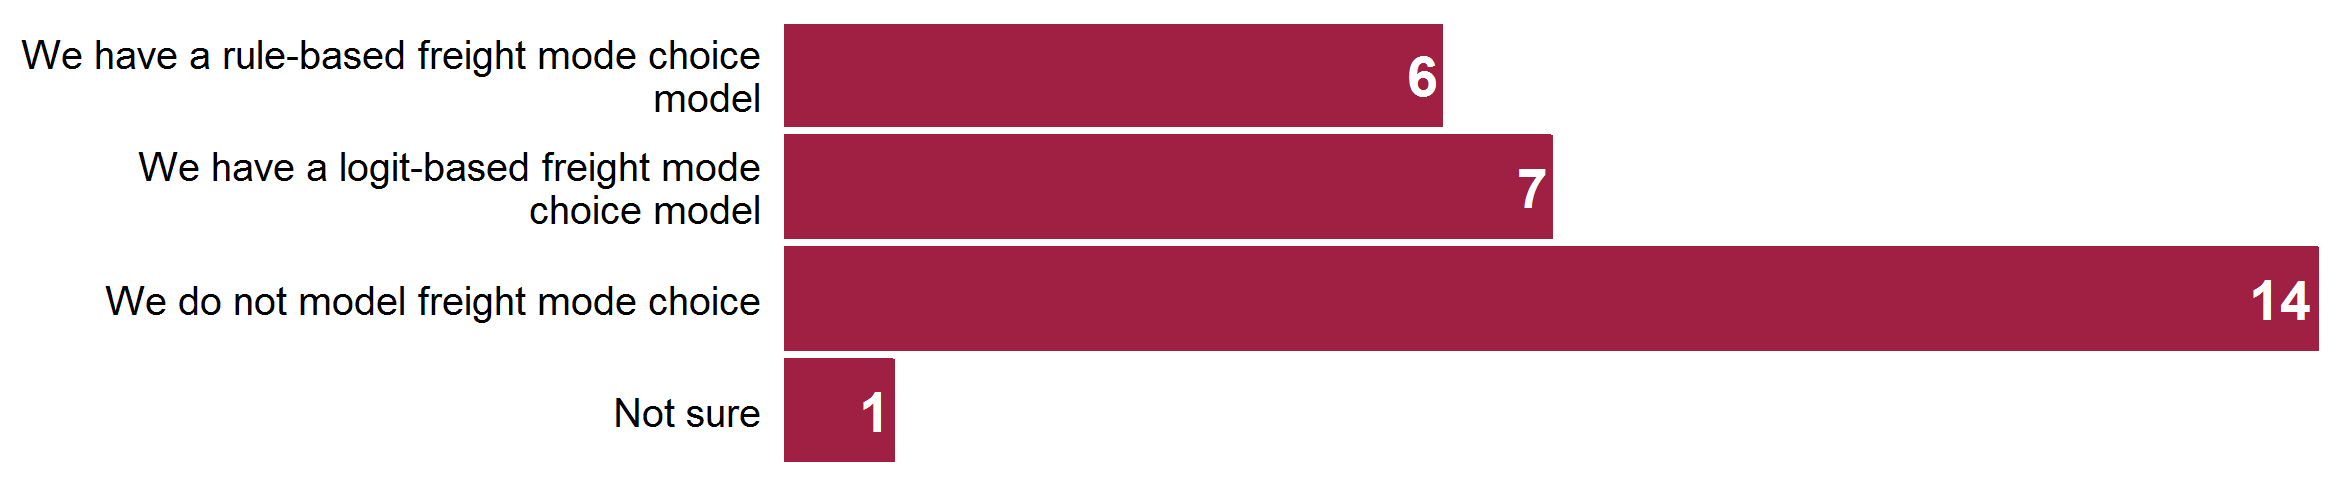
\includegraphics[width=6.4in]{graphics/25-freight-mode-choice}
\caption[Frequency of freight mode choice models]{Frequency of freight mode choice models (multiple answers allowed)}
\label{fig:freight-mode-choice}
\end{figure}

Logit-based freight mode choice models were implemented by Florida, Georgia, Illinois, Ohio, Oregon, Texas, and Virginia. While such models provide rich information on driving factors for mode choice, data limitations often make it challenging to reasonably estimate these models. Many of these logit-based models are designed as so-called freight diversion models (i.e., they model the shift from one mode, such as truck, to another mode, such as rail). Starting with the observed mode share and modeling only the potential shift from one mode to another is a powerful way to deal with data limitations in freight modeling while maintaining some freight mode sensitivities to policy scenarios. Ohio and Oregon use a combination of both rule-based and logit-based mode choice models. About half of the 26 states that model freight long-distance flows do not model freight mode choice at all, but instead generate truck flows only.

Of the 11 statewide models that represent freight mode choice, all include truck and rail as modal options (Figure \ref{fig:freight-long-distance-modes}). Water and Air are modeled in eight and seven states, respectively. California, Ohio, Oregon and Utah even model pipelines, a flow that is inherently difficult to represent because it has the least amount of data available. Accordingly, FAF decided to merge the pipeline and unknown modes. One other mode was mentioned by Utah, where truck-rail intermodal represents a separate mode. It was known that this mode is also used in other states, such as Ohio and Texas, although they did not state so because it was not explicitly requested in the survey.

\begin{figure}   % 26
\centering
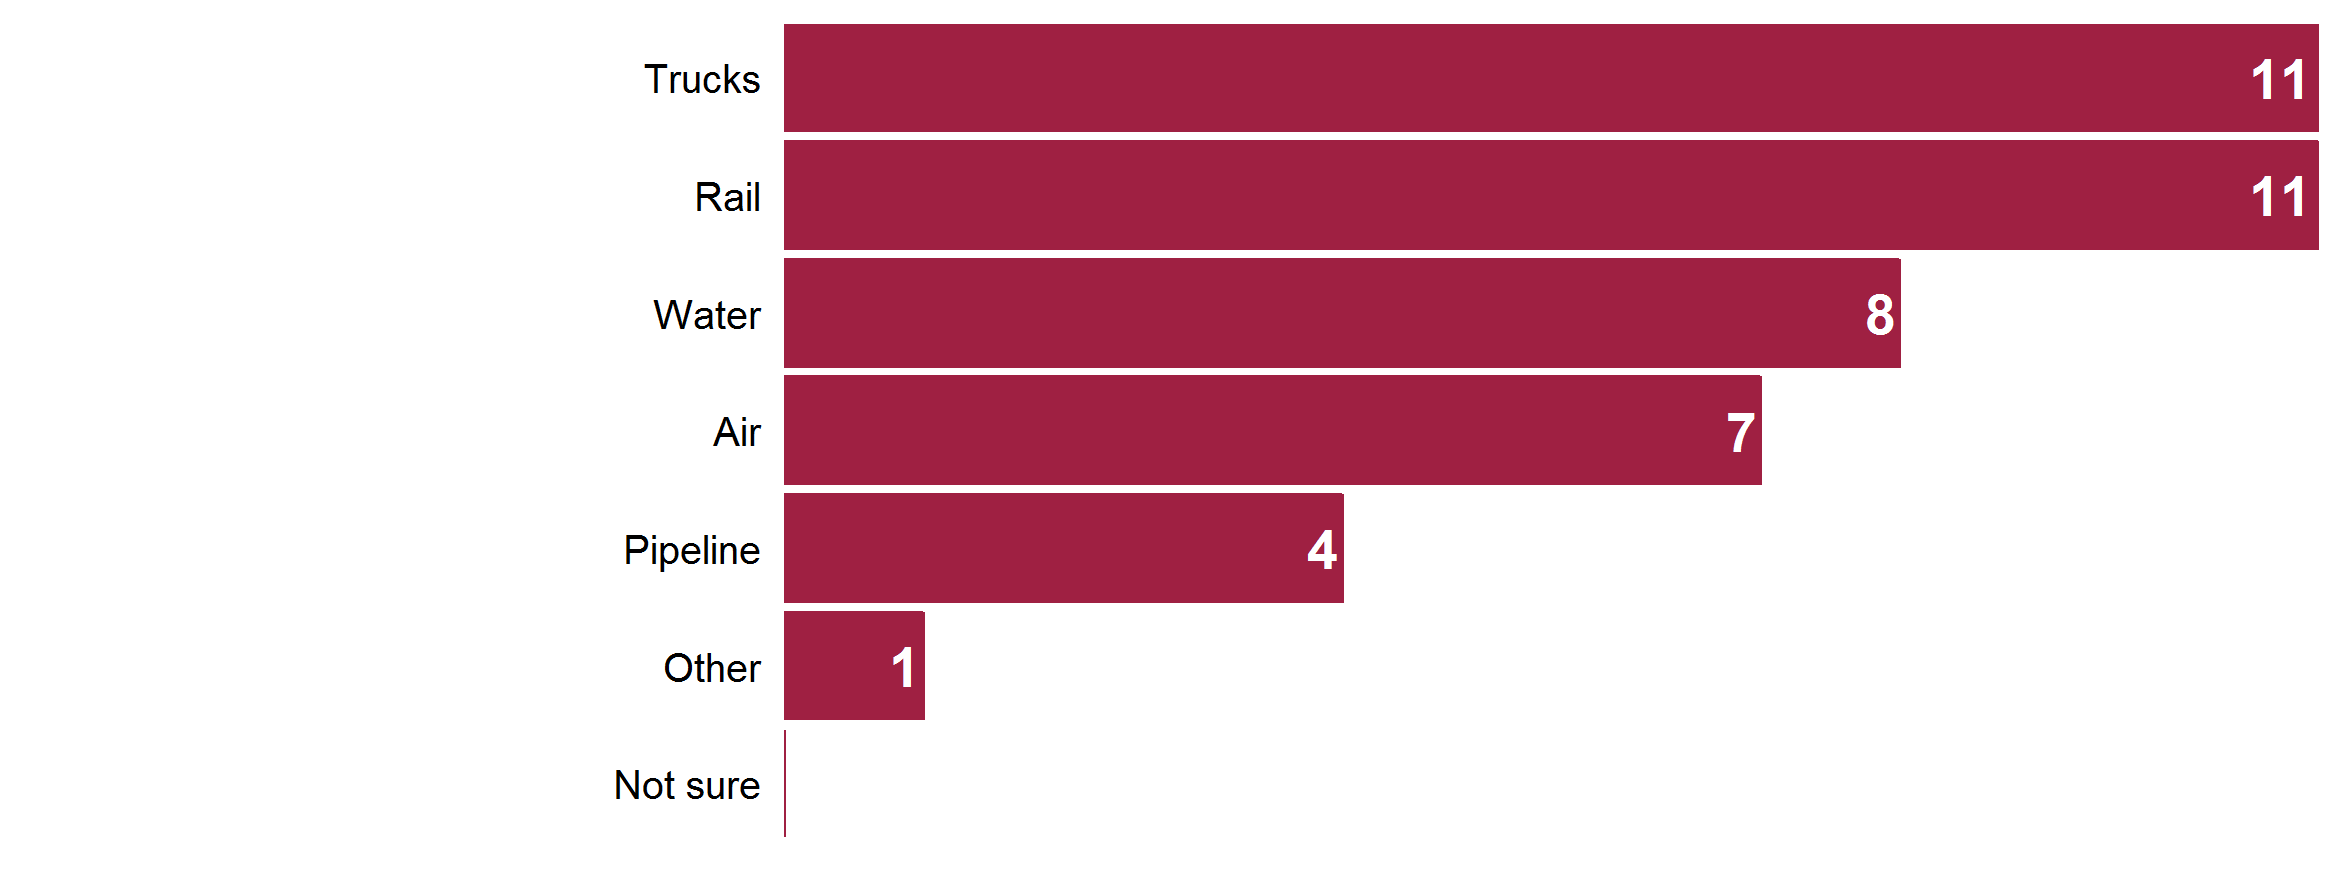
\includegraphics[width=6.4in]{graphics/26-freight-long-distance-modes}
\caption[Modes represented in long-distance freight mode choice models]{Modes represented in long-distance freight mode choice models (multiple answers allowed)}
\label{fig:freight-long-distance-modes}
\end{figure}

\section{Economic models}

Traditionally, statewide transportation models worked with static socio-economic input data. Given the large uncertainty of economic forecasts, many states have moved towards integrating their transportation model with economic forecast models. While such models are not capable of reliably forecasting the future, they add the flexibility of providing socio-economic input data for alternative futures. Many states have a forecast they assume to be the most likely forecast. In addition, each scenario is run with a low-growth forecast and a high-growth forecast, which may be, for example, 5--25 percent above or below the expected growth rate. Having various forecasts allows states to capture some of the uncertainty of future growth, and enables them to test if scenarios are viable under alternative growth scenarios.

In addition to growth rate adjustments, most economic forecast models also represent the interdependencies between various industries and population. If the auto industry enjoys continued growth, firms delivering parts to that industry would grow accordingly. If the unemployment rate in an area is growing the population will likely grow at a slower pace. Accounting for such interdependencies makes stories behind future scenarios richer and increases consistency, and thereby, credibility.

The frequency of economic forecast models is summarized in Figure \ref{fig:economic-model-frequency}. Externally prepared commercial forecasts are the most frequent source of future socio-economic data, closely followed by forecasts developed by other state agencies. Illinois and New Hampshire do not need or use an economic forecast or model, as they only apply the model in the base year.

\begin{figure}   % 27
\centering
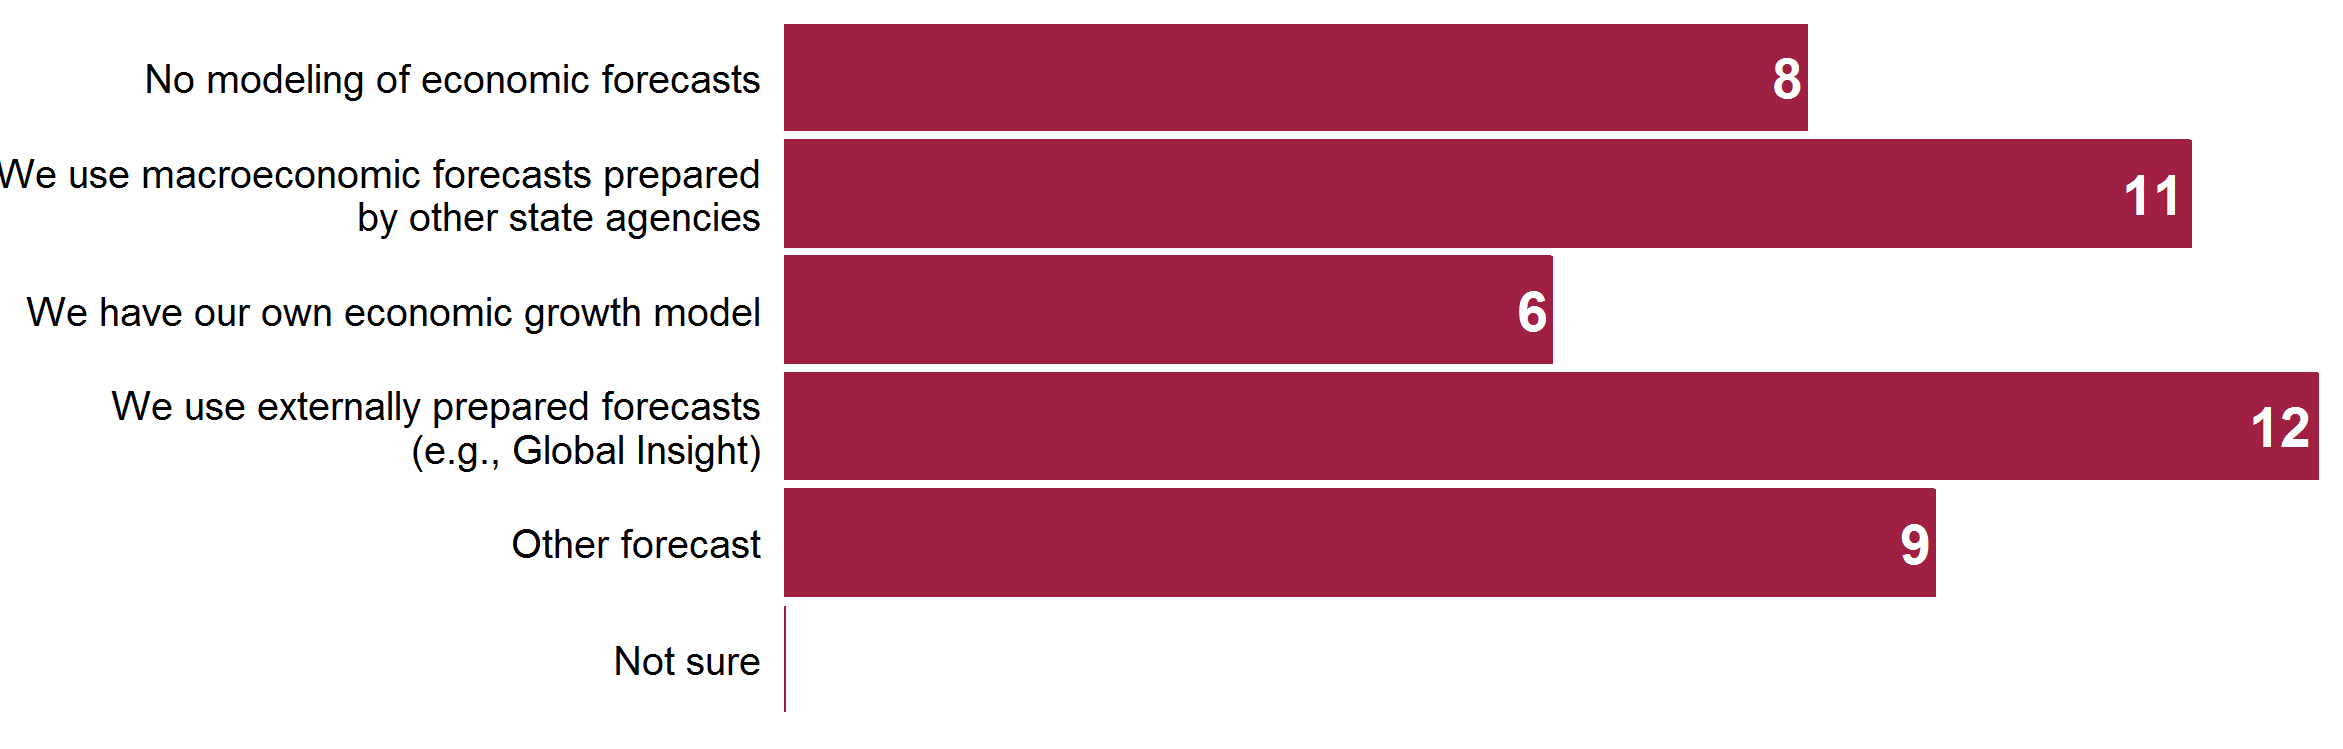
\includegraphics[width=6.4in]{graphics/27-economic-model-frequency}
\caption[Frequency of economic forecast models]{Frequency of economic forecast models (multiple answers allowed)}
\label{fig:economic-model-frequency}
\end{figure}

Respondents in the nine states who selected ``Other forecast'' mentioned that they:
\begin{itemize}
\item Prepare their own forecast,
\item Use the REMI economic forecasting model,
\item Derive population growth forecasts from Longitudinal Employment Household Dynamics (LEHD) and Woods \& Poole population trends, and
\item Work with universities or local consultants to generate forecasts.
\end{itemize}

The agency that operates the transportation model creates their own forecast of socioeconomic data in only six states (or 18 percent of those that have statewide models). This is not to be criticized, as economic forecasts are challenging. However, this likely limits the number of growth rate scenarios that can be run with the transportation model. While a few alternative growth scenarios may be sufficient, agencies that operate their own models may work with a larger number of different growth assumptions.

The distribution of base and future model years are visualized in Figure \ref{fig:base-and-future-years}. Base years cluster around 2010, as expected, while future years dominate in 2015, 2020, 2030, 2035 and particularly in 2040. Beyond that, New York models 2044, California 2050 and Nevada 2060. Several models can provide forecasts for any future year within their model time frame. This is achieved by interpolating between five or 10-year model runs. While this approach assumes a somewhat artificial linear growth between two modeled years, interpolation provides additional data for years the model cannot be run.

\begin{figure}   % 28
\centering
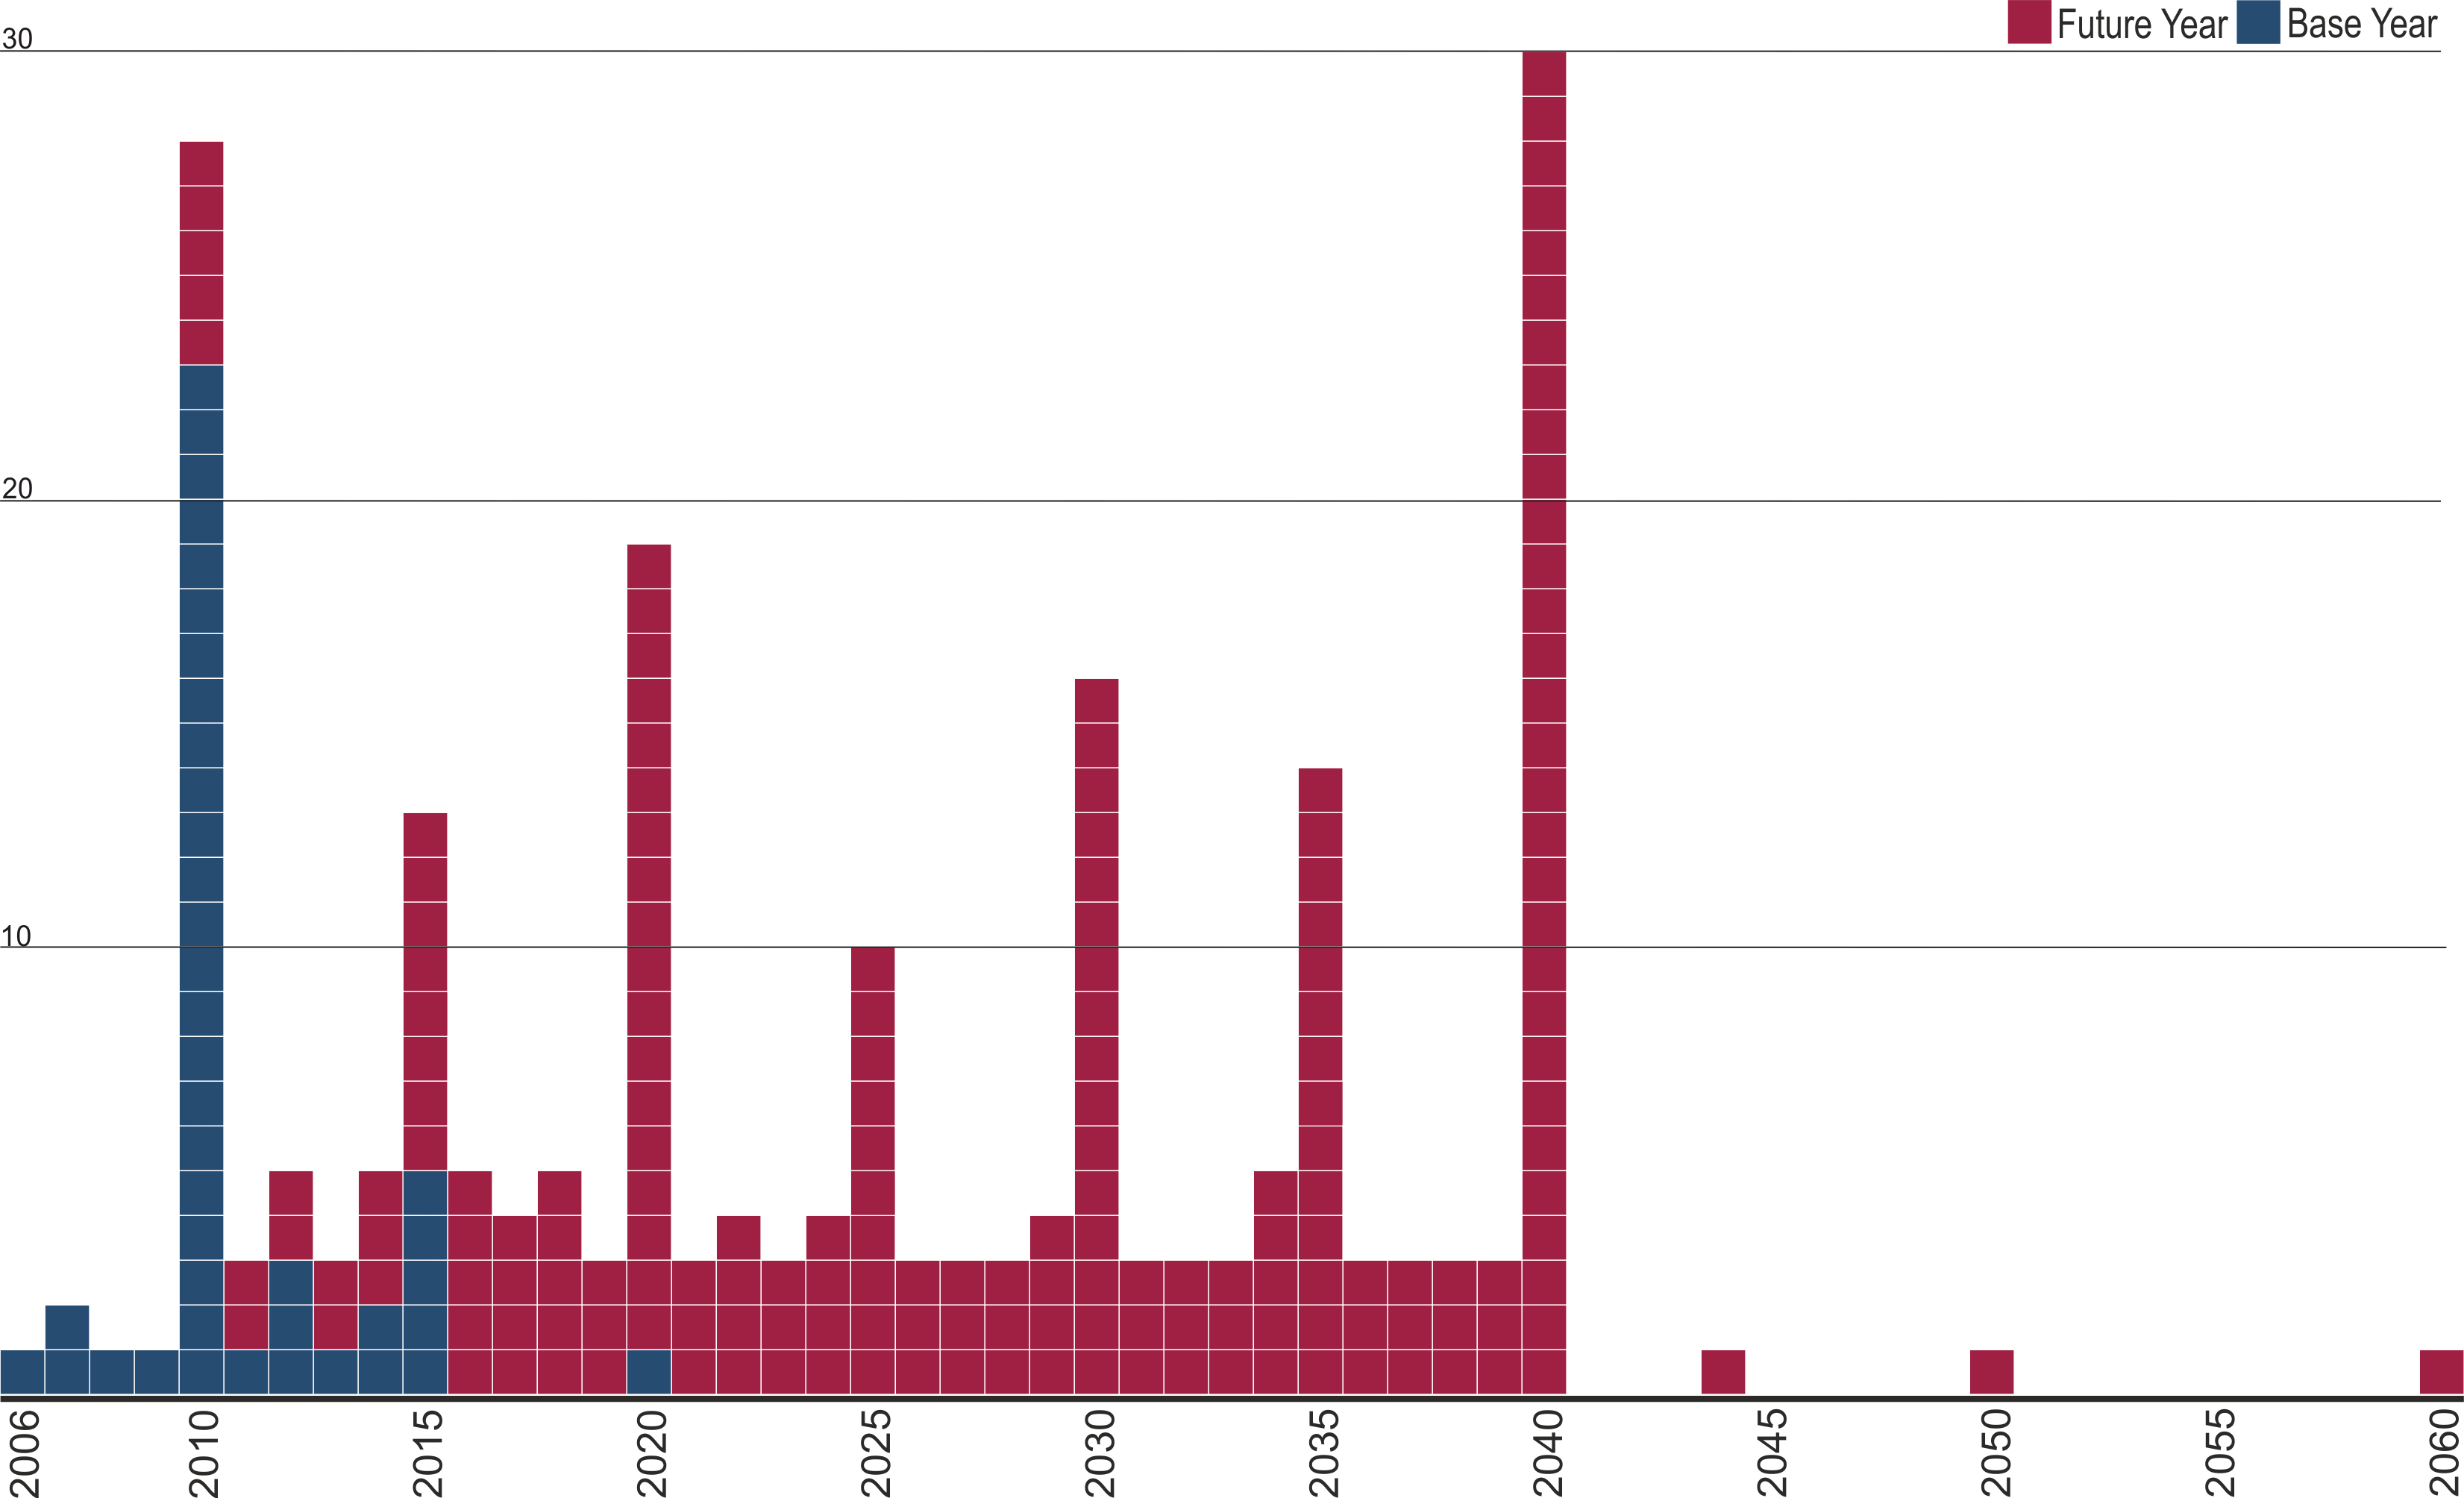
\includegraphics[width=6.4in]{graphics/28-base-and-future-years}
\caption{Distribution of base and future years in statewide models}
\label{fig:base-and-future-years}
\end{figure}

\section{Land use models}

Land use models can be integrated with travel demand models to reflect the interactions between the transportation system and land use development. Both households and businesses prefer locations with higher accessibilities, all else being equal, and are therefore influenced by travel times forecasted using transportation models. The location choices of households, businesses, and developers, in turn, influences the origins and destinations of travel demand calculated in the transportation model. The integration of land use with transportation models has proven to improve model sensitivities in scenario analyses \citep{conder02}. This integration has been visualized schematically in Figure \ref{fig:landuse-transport-feedback}.

\begin{figure}
\centering
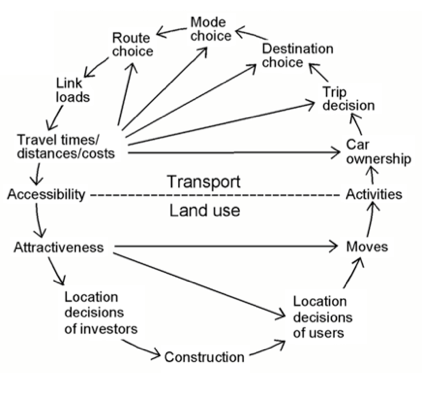
\includegraphics[scale=0.5]{graphics/29-land-use-transport-feedback-cycle}
\caption[Land use-transport feedback cycle]{Land use-transport feedback cycle (Source: \cite{wegener94})}
\label{fig:landuse-transport-feedback}
\end{figure}

Empirical research has shown that transportation systems influences land-use decisions \citep{hansen59}, and, therefore, the allocation of socio-economic data. While the static land-use forecast may be appropriate in the base scenario (often called business-as-usual scenario), the forecast of population and employment may be unrealistic in scenarios in which travel times change significantly. For example, if the model is used to test the expansion of a rail line, households may decide to relocate because the rail line may make certain neighborhoods more attractive. As another example, if congestion increases substantially, urban sprawl might be slowed down.

Land use modeling is more common for urban models, and thus, only two states, Ohio and Oregon, have operational land use models at the statewide level (Figure \ref{fig:integrated-models}). Nevada and Indiana are currently developing land use models.

\begin{figure}   % 30
\centering
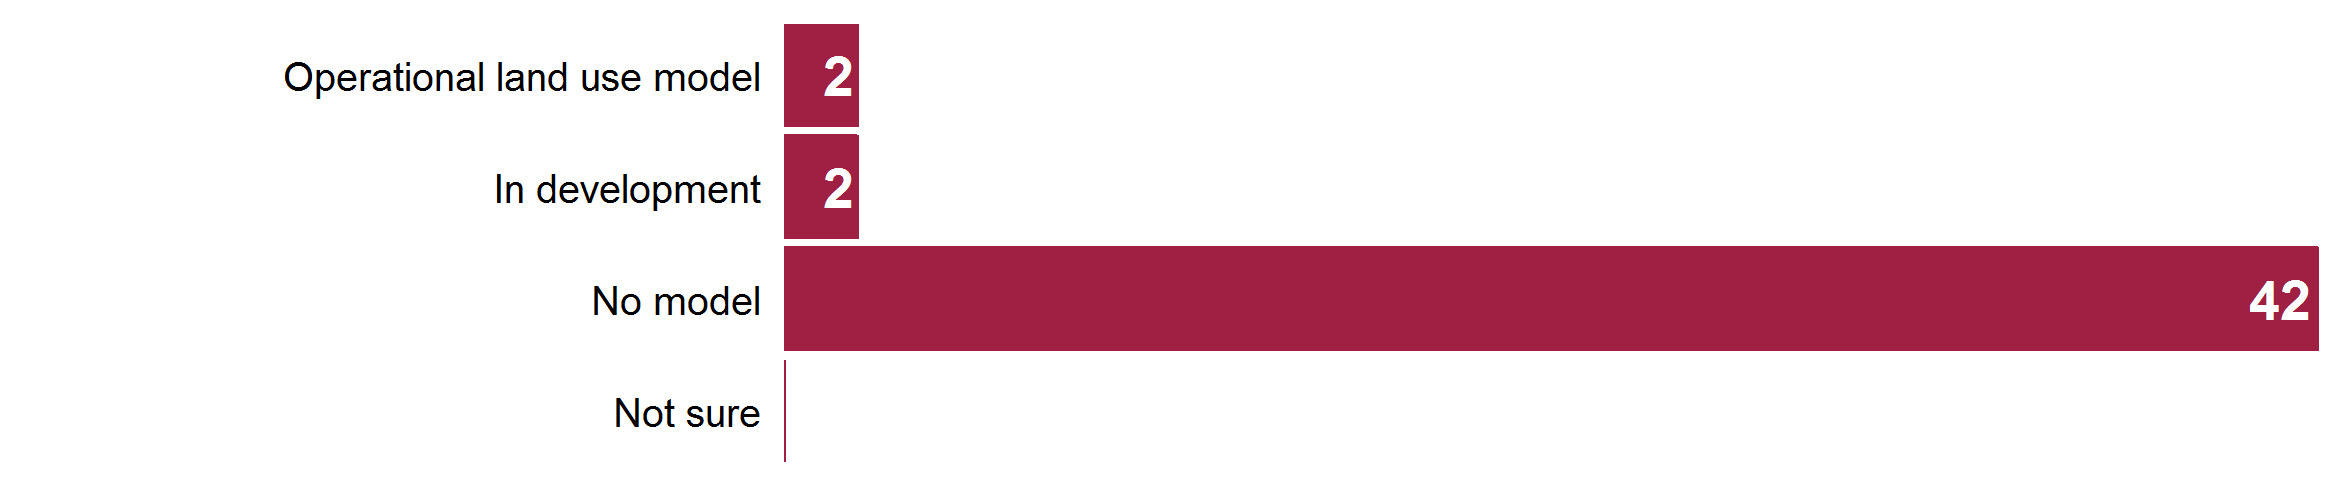
\includegraphics[width=6.4in]{graphics/30-integrated-land-use-transport-models}
\caption{Frequency of integrated land use-transportation models at the statewide level}
\label{fig:integrated-models}
\end{figure}

A clustering of land use models of Oregon/Nevada and Indiana/Ohio can be seen in Figure \ref{fig:land-use-model-states}, which may be entirely coincidental. While at least three more states (California, Florida and Maryland) have operational land use models as well, they have not been integrated with the official version of the statewide transportation model, and therefore do not appear in Figures \ref{fig:integrated-models} and \ref{fig:land-use-model-states}.

\begin{figure}   % 31
\centering
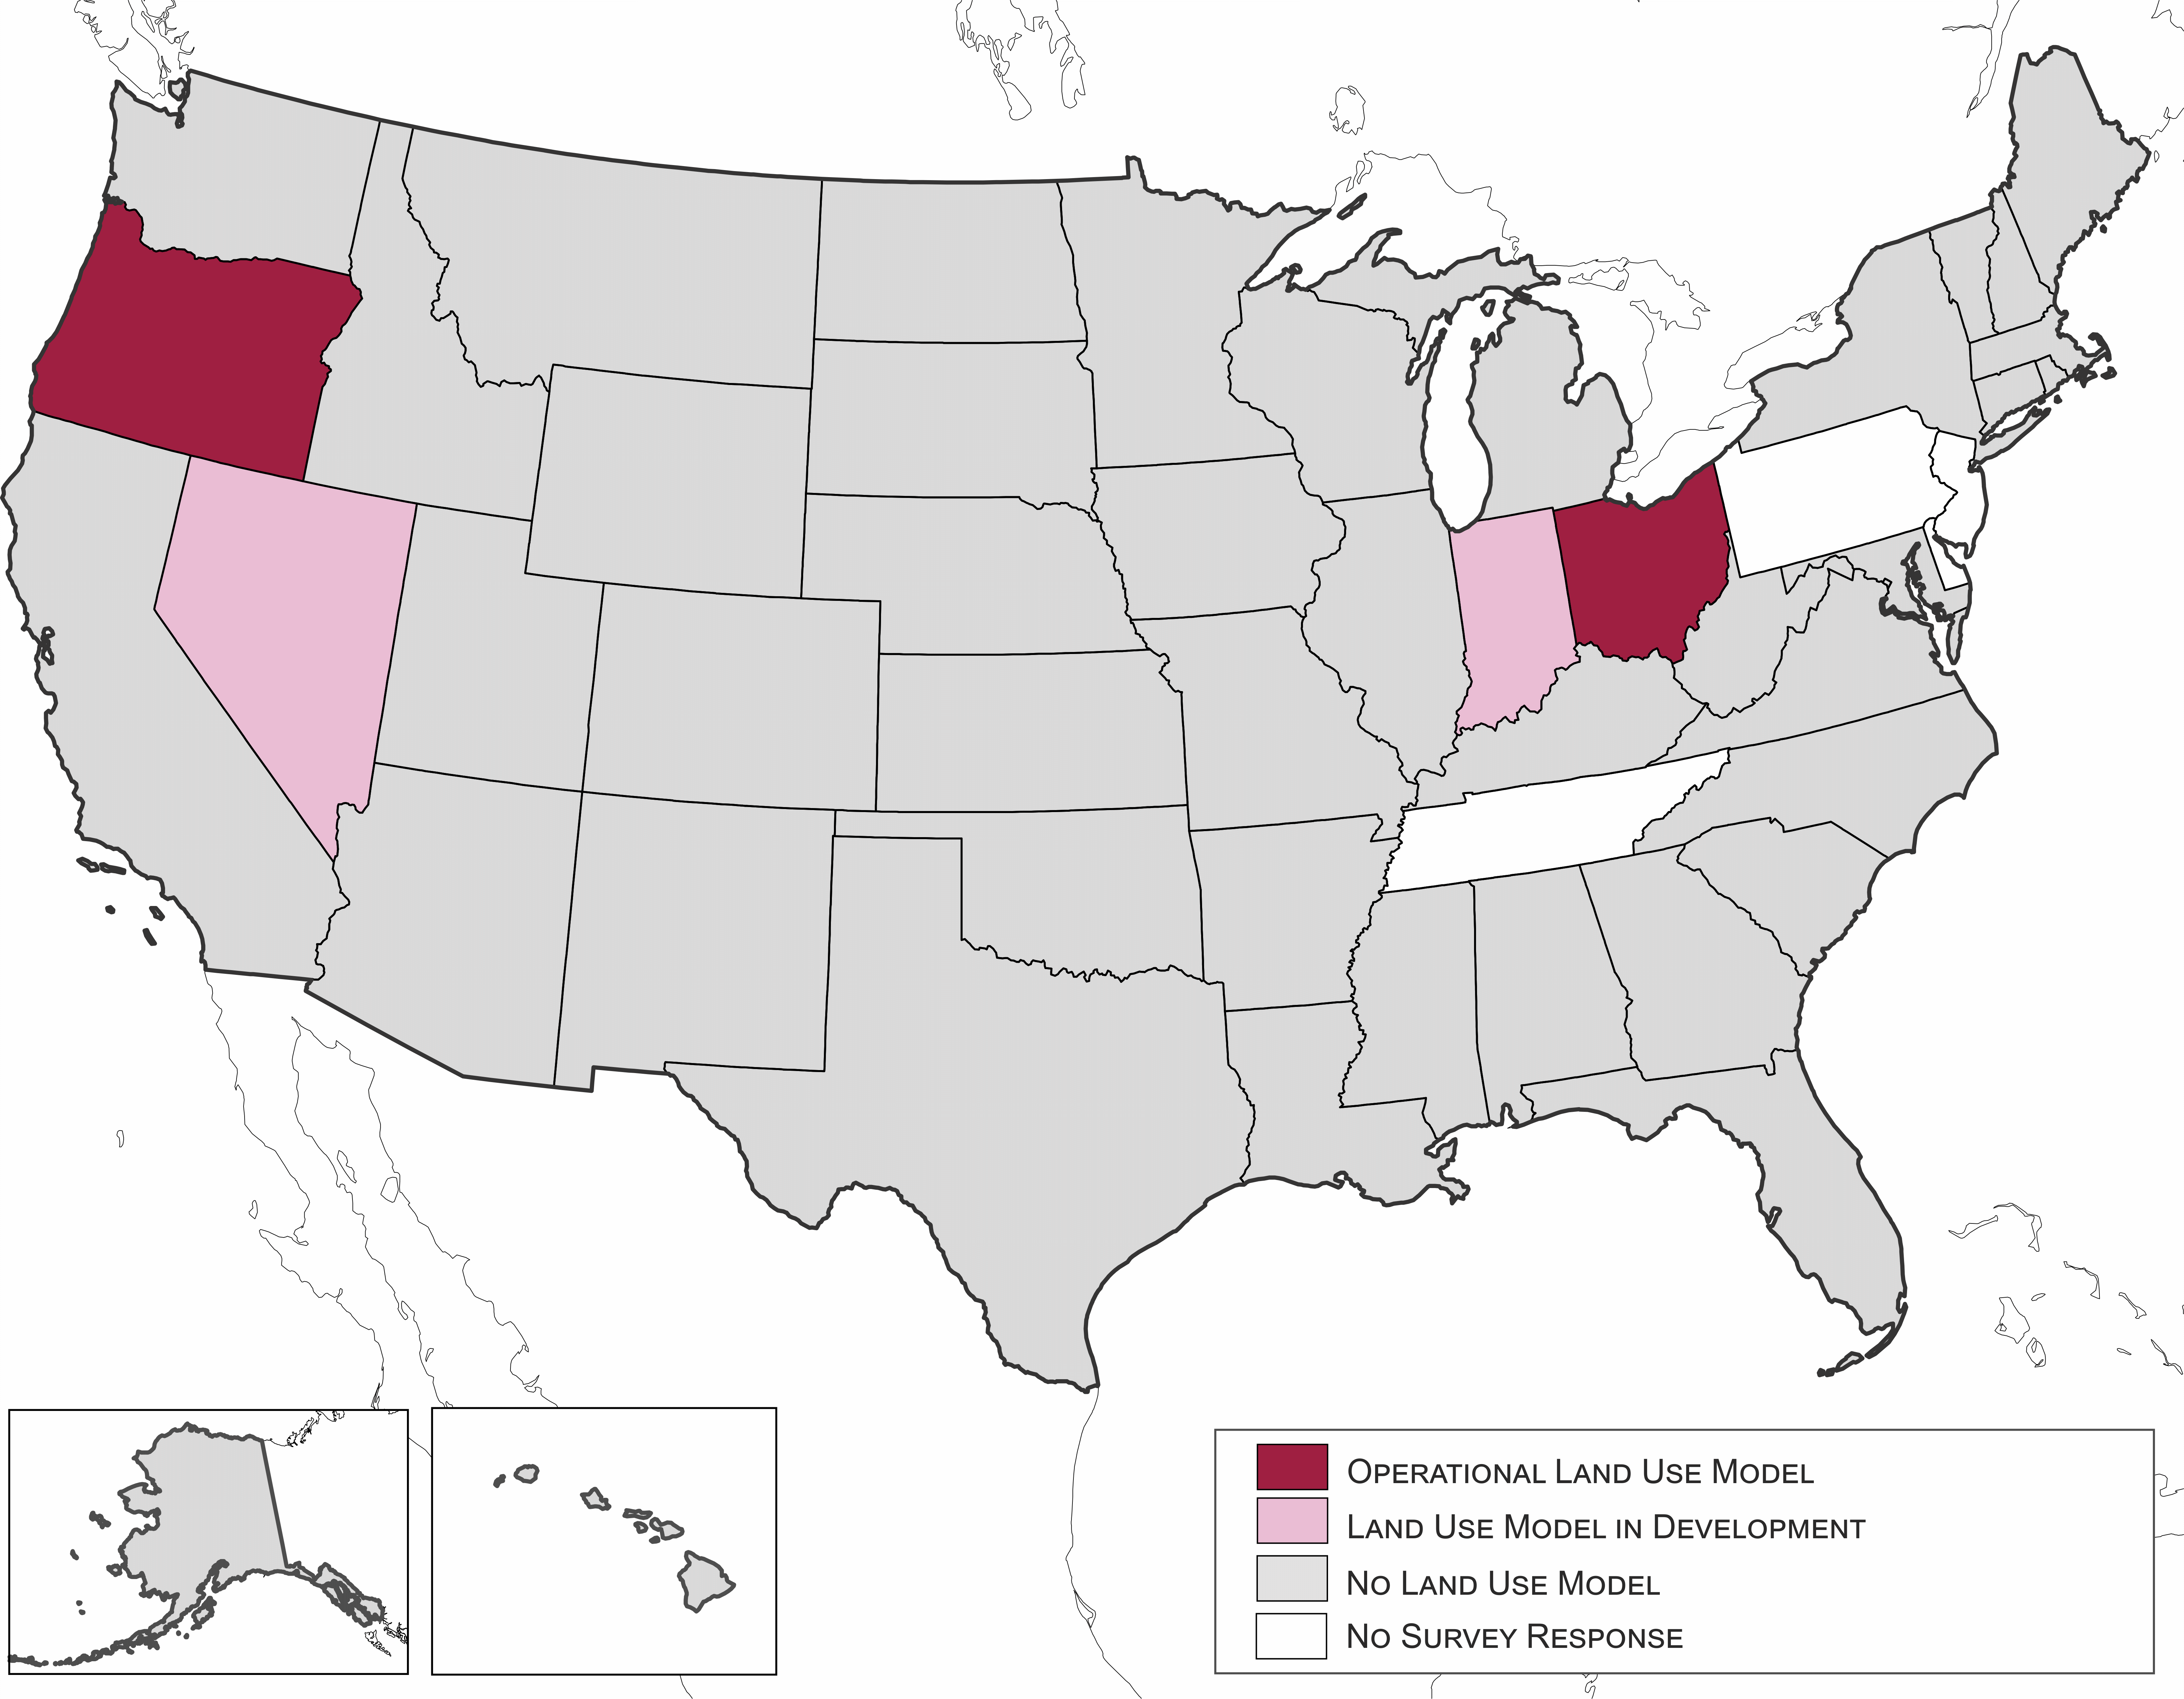
\includegraphics[width=6.5in]{graphics/31-land-use-model-states}
\caption{Distribution of states with land use models}
\label{fig:land-use-model-states}
\end{figure}

\section{Environmental impact models}

Nine states explicitly model the environmental impacts of traffic flows, as shown in Figure \ref{fig:environmental-model-frequency}. This number is relatively small, given that it is common practice to model environmental impacts with urban models. All cases reported referred only to air quality. In research environments, models to analyze the impact on water quality have been developed (see \S\ref{sec:chesapeake-bay-megaregion-model} and \cite{baker07}), though such models have not yet been applied in practice.

\begin{figure}   % 32
\centering

\includegraphics[width=6.4in]{graphics/32-environmental-model-frequency}
\caption{Frequency of environmental impact modeling within statewide models}
\label{fig:environmental-model-frequency}
\end{figure}

The spatial distribution of states with environmental impact models is shown in Figure \ref{fig:environmental-model-states}. It is notable that all West Coast states (of the lower 48 states) model environmental impacts, for environmental issues have traditionally been given more attention than in many other parts of the country. Two Southern states and Michigan also model environmental impacts, and a New England cluster can be seen as well.

\begin{figure}   % 33
\centering
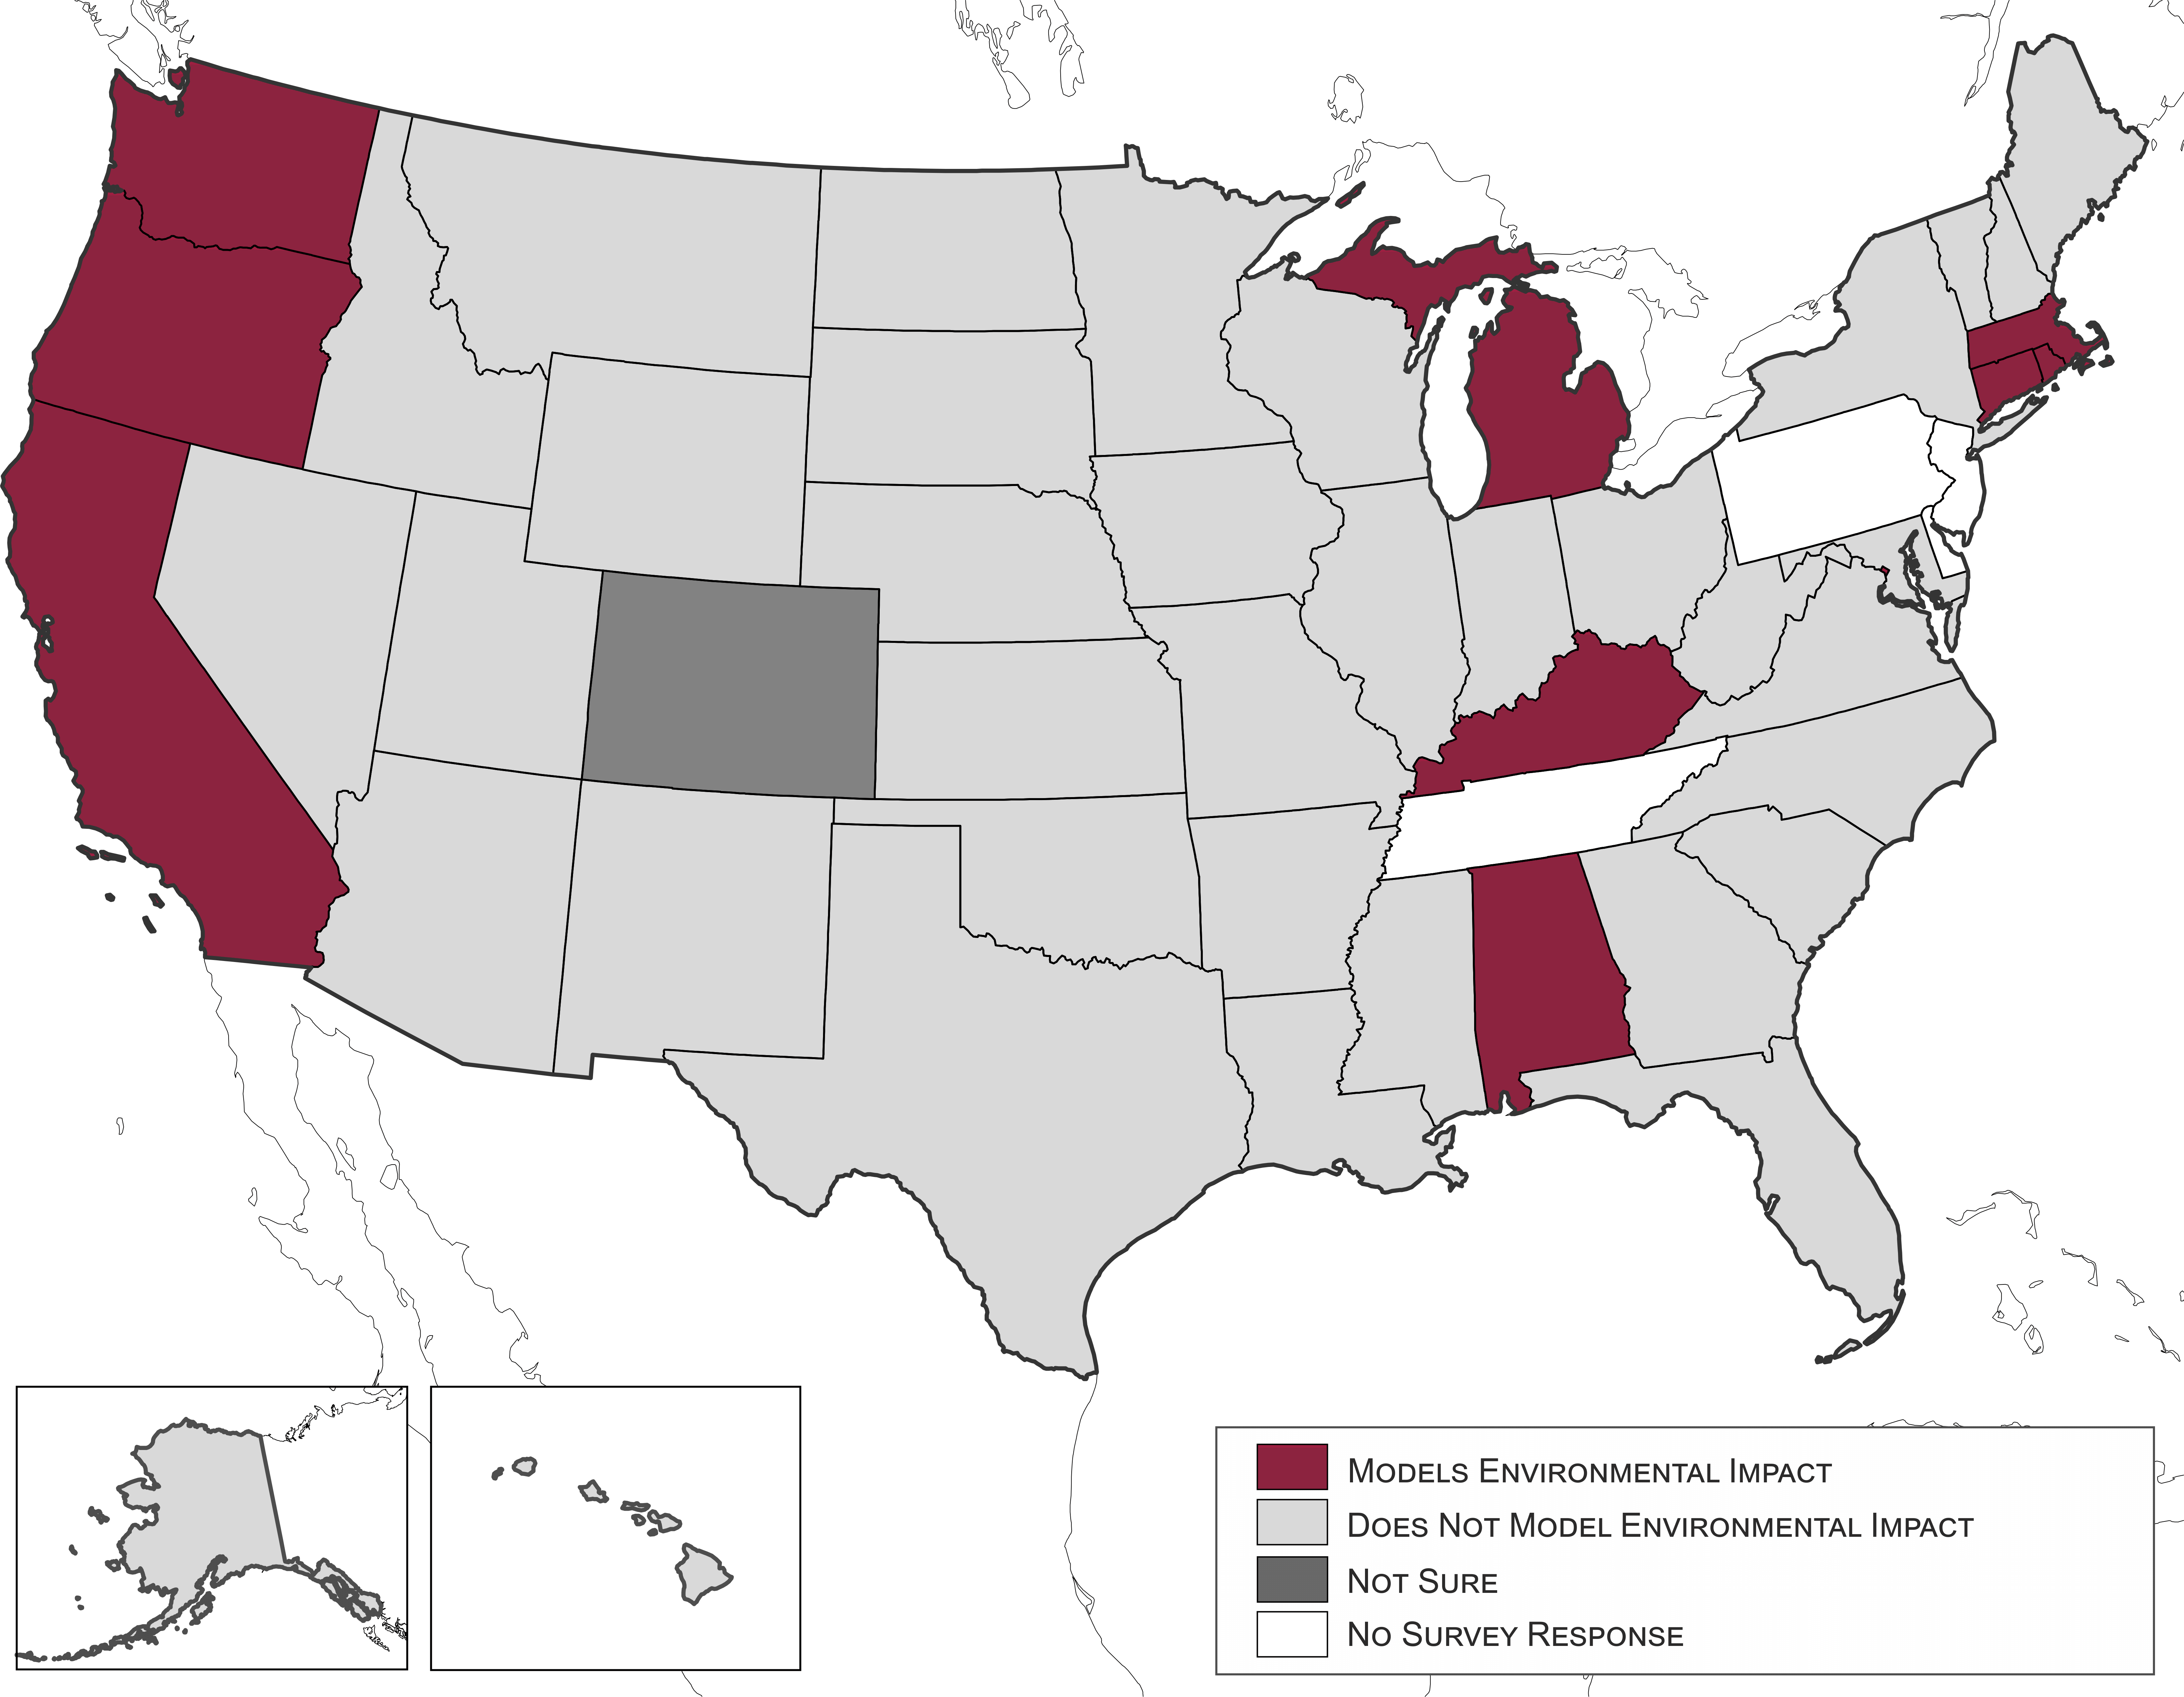
\includegraphics[width=6.5in]{graphics/33-environmental-model-states}
\caption{Distribution of states that model environmental impacts}
\label{fig:environmental-model-states}
\end{figure}

Most states that model environmental impacts use the MOVES model, as shown in Figure \ref{fig:environmental-impact-models}. This model is provided by the Environmental Protection Agency (EPA) at no cost, and is widely accepted as the U.S. standard for modeling air pollutants, greenhouse gases, and air toxics generated by mobile sources. Oregon uses MOVES in combination with their own greenhouse gas model (GreenStep), and Kentucky uses both MOVES and its predecessor, MOBILE. EMFAC is used in California only, based upon emission rates provided by California EPA's Air Resources Board.

\begin{figure}   % 34
\centering

\includegraphics[width=6.4in]{graphics/34-environmental-impact-models}
\caption[Frequency of environmental impacts models]{Frequency of environmental impacts models (multiple answers allowed)}
\label{fig:environmental-impact-models}
\end{figure}

The types of emissions covered are listed in Figure \ref{fig:emissions-modeled}. CO\textsubscript{2}, NO\textsubscript{x} and PM are the most common emissions modeled. Oregon and Washington are the only two states that calculate noise emissions, a significant factor that impacts human health and well-being \citep{decoensel05}. Other analyzed emissions reported included VOC (Connecticut, Kentucky, Massachusetts), CO (Massachusetts) and O\textsubscript{3} (Rhode Island).

\begin{figure}   % 35
\centering
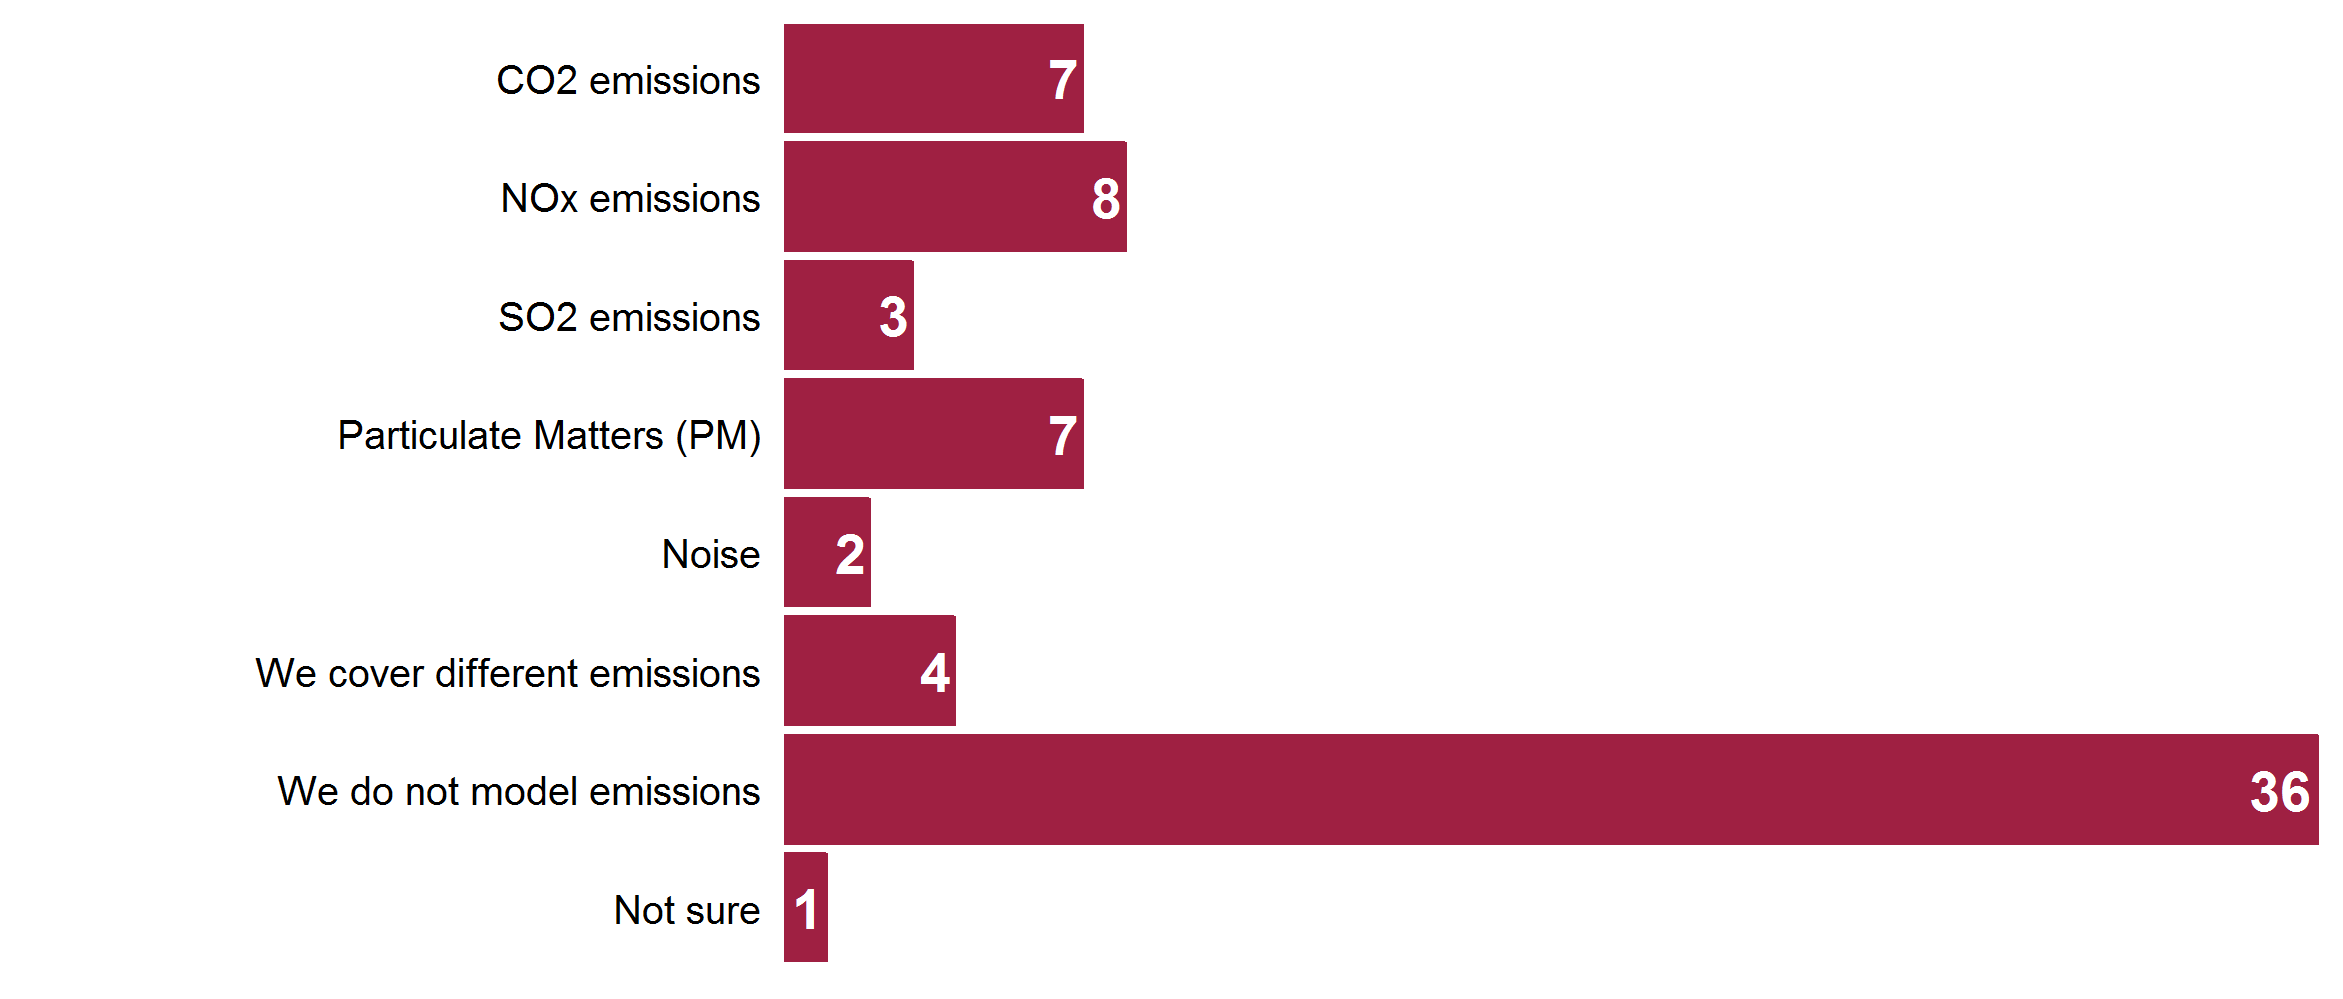
\includegraphics[width=6.4in]{graphics/35-emissions-modeled}
\caption[Emissions modeled with statewide models]{Emissions modeled with statewide models (multiple answers allowed)}
\label{fig:emissions-modeled}
\end{figure}

\section{Resources}

Agencies that operate statewide models were asked about the resources they have invested in model development and application. The first question asked for the number of full-time equivalent employees. Answers ranged from zero to six full-time equivalent employees, with an average of 1.6, as shown in Figure \ref{fig:staffing}. Note that each bar represents a range; for example, the left-most bar stands for five agencies that have between zero and 0.5 full-time equivalent employees.

\begin{figure}   % 36
\centering
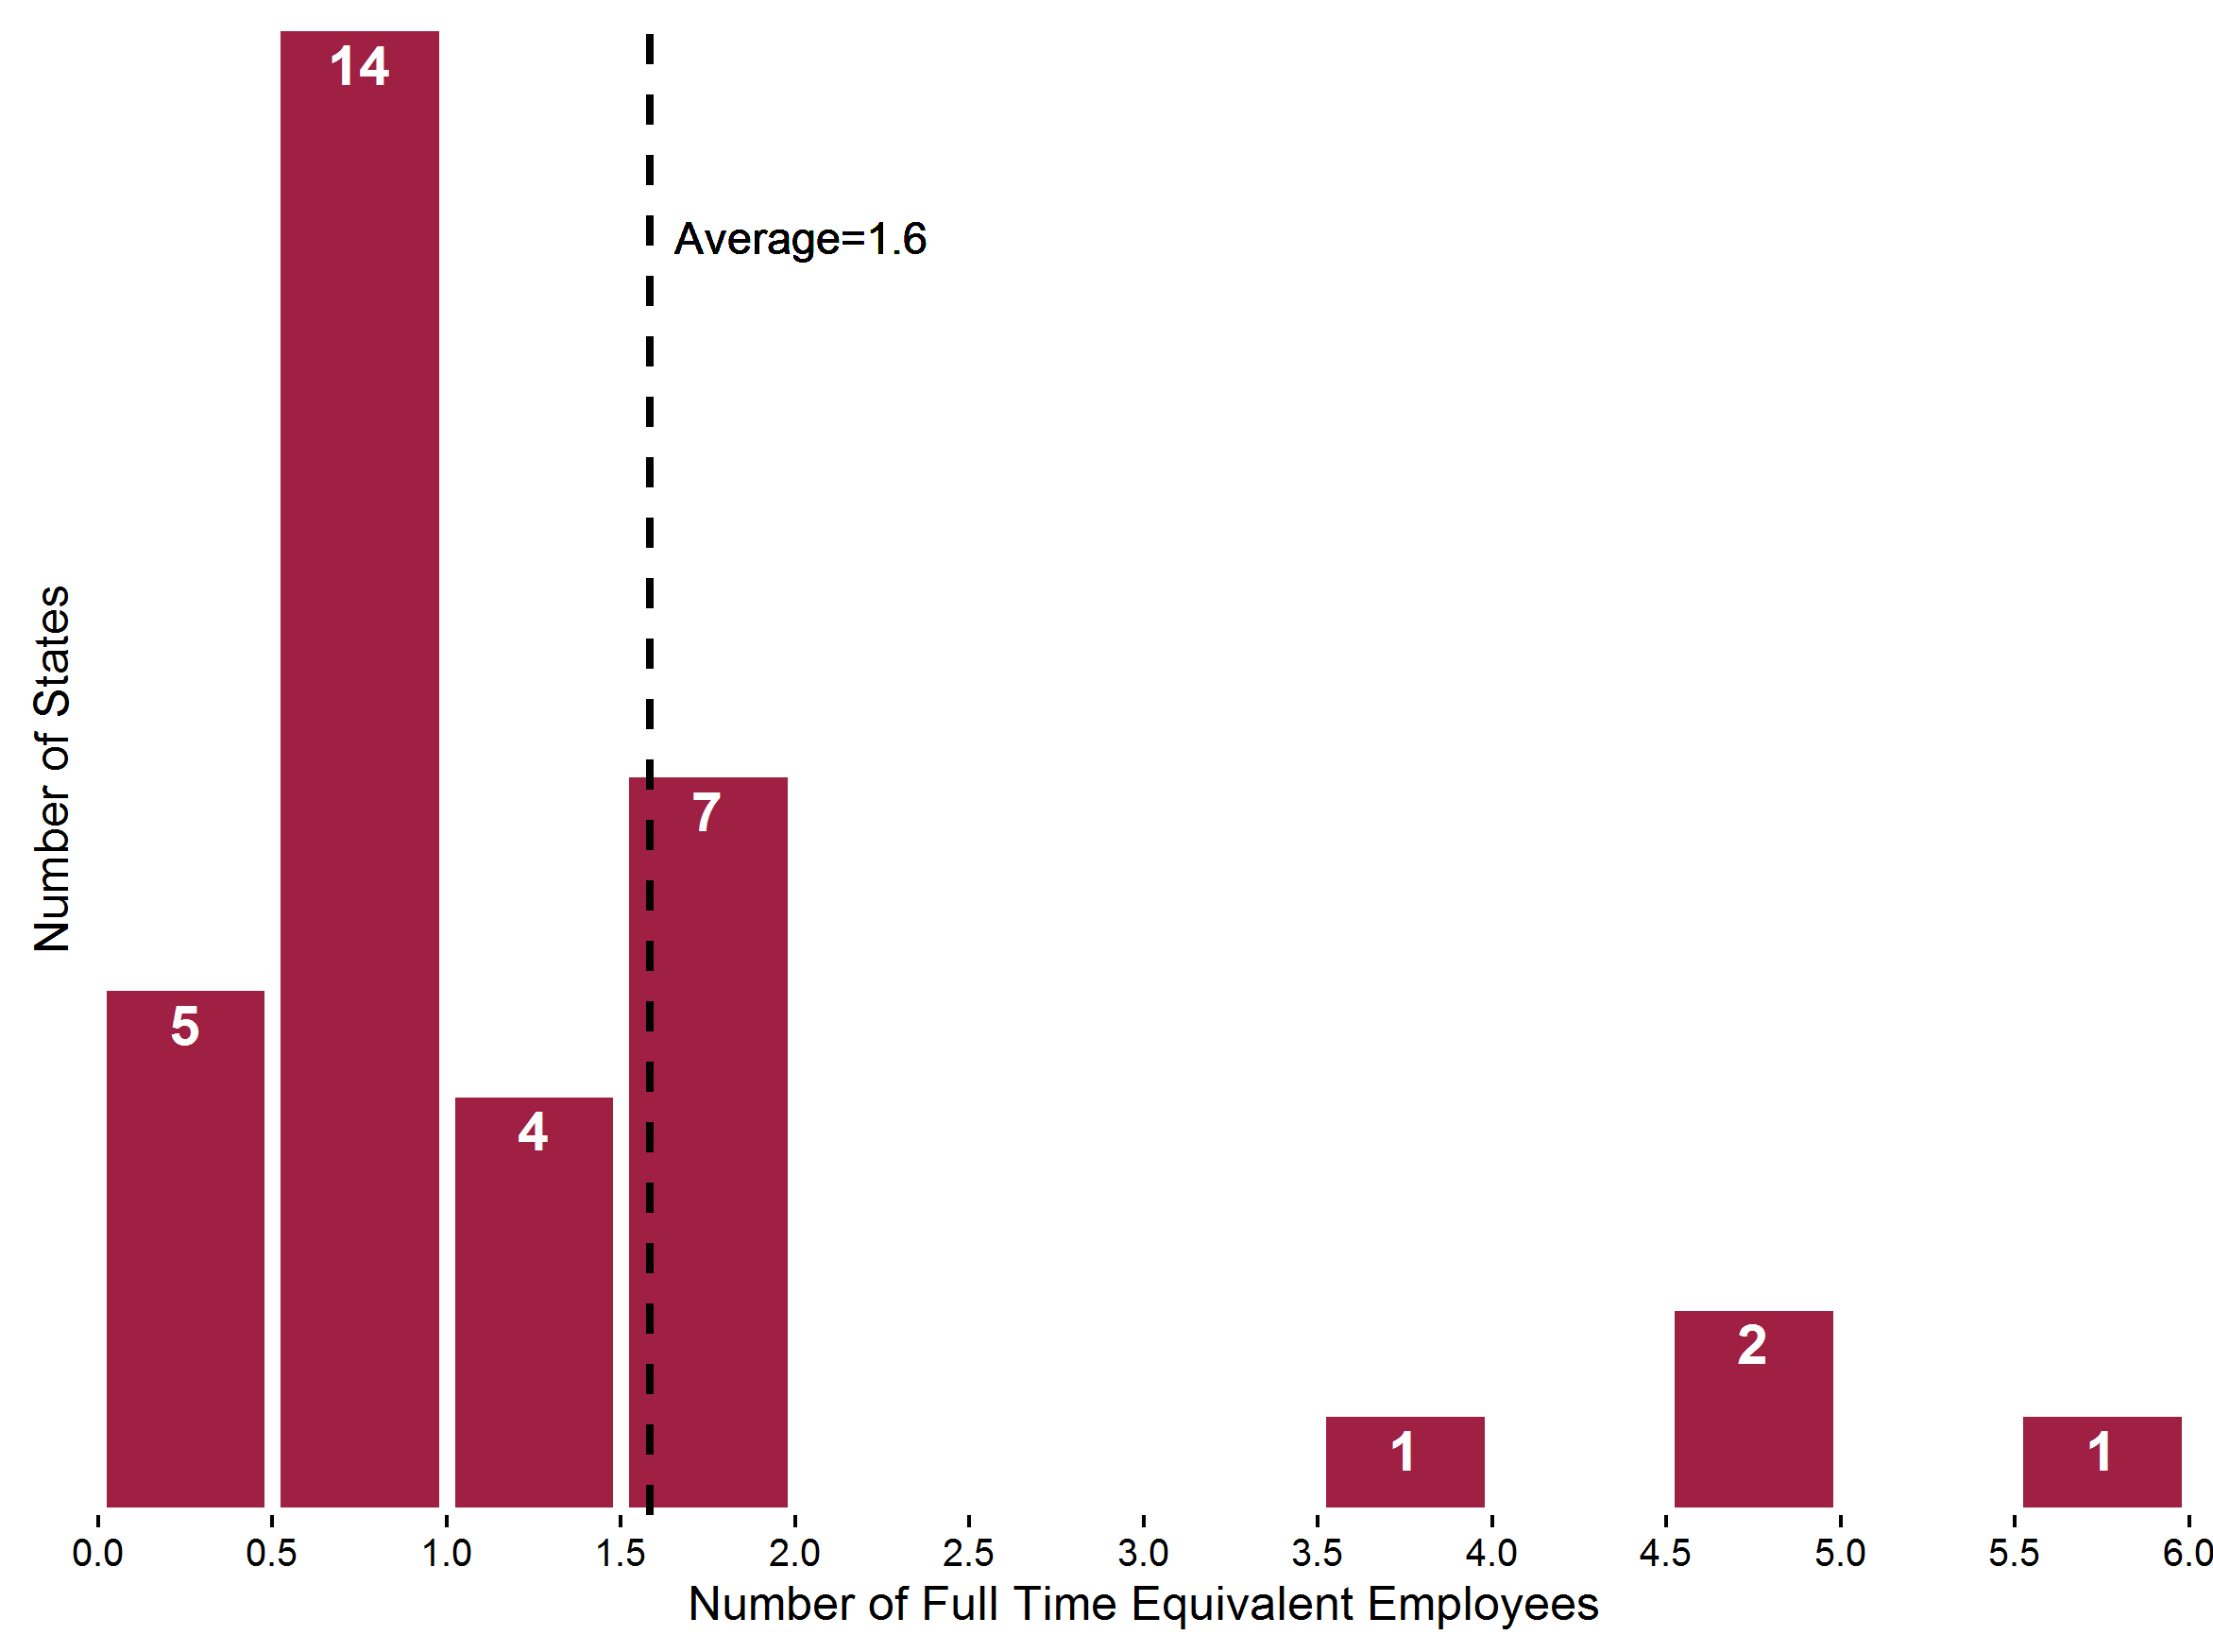
\includegraphics[width=5.8in]{graphics/36-staffing}
\caption{Number of full-time equivalent employees working on statewide modeling}
\label{fig:staffing}
\end{figure}

For model development, a relatively large share of resources (71 percent) were allocated to consultants on average, plus another eight percent being allocated to universities (Figure \ref{fig:resource-allocation}). Only 20 percent of the resources were invested in-house or for partner agencies. On the one hand, this means that a lot of expertise in model development is found outside the state agency. On the other hand, it might be considered neither cost efficient nor practical to train staff to build a model, a task faced by the agency maybe every 10 to 20 years.

\begin{figure}   % 37
\centering
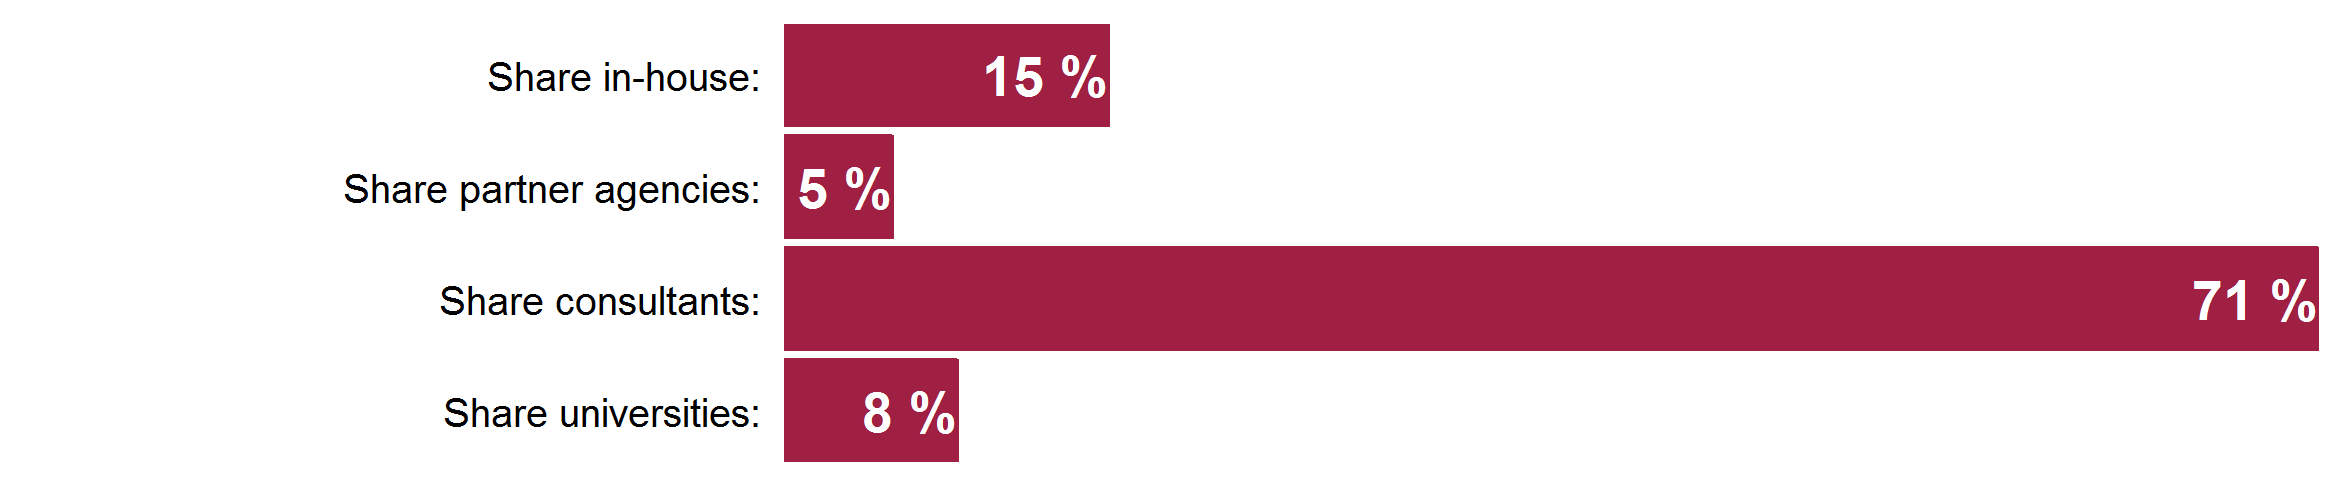
\includegraphics[width=6.4in]{graphics/37-development-resource-allocation}
\caption{Resource allocation for model development}
\label{fig:resource-allocation}
\end{figure}

For model application, the percentages are almost completely reversed, as shown in Figure \ref{fig:application-resource-allocation}. In-house and partner agencies on the average conduct 60 percent of the model application work. Compared to model development, the share for consultants and universities drops in half. While this general trend was expected, the combined 39 percent of outside support for model development is rather large. Except for highly specialized scenarios or short-term staff shortages, state agencies would benefit greatly from avoiding outsourcing of model applications, and instead building this capacity in-house.

\begin{figure}   % 38
\centering
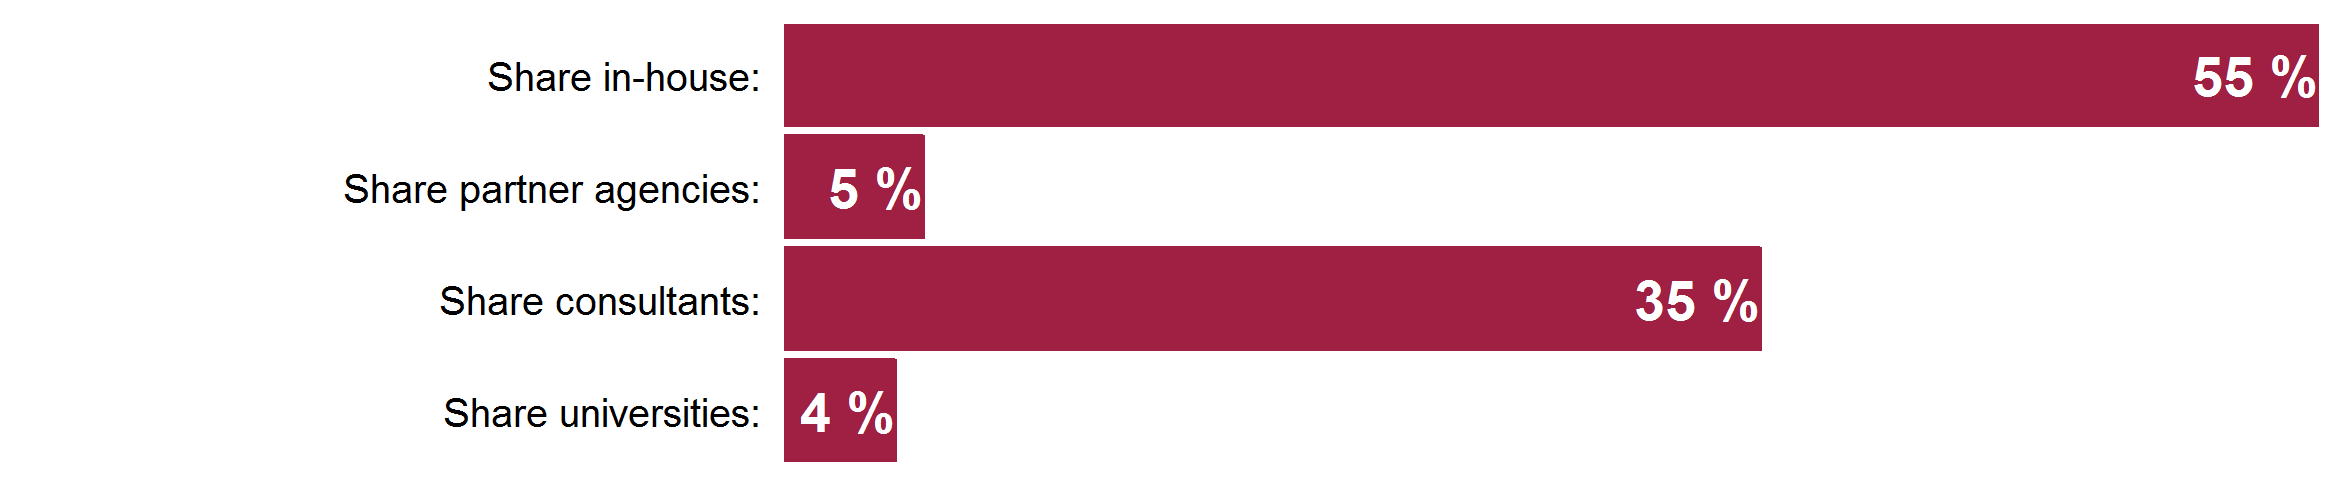
\includegraphics[width=6.4in]{graphics/38-application-resource-allocation}
\caption{Resource allocation for model application}
\label{fig:application-resource-allocation}
\end{figure}

Finally, the questionnaire asked how much money was invested into the model over the past several years. The estimate does not include costs for staff within the agency, but only expenditures for data purposes, software licenses, and outside help. Several states noted that it was difficult to retrieve these numbers, and that they likely had spent more money than reported. In some cases, the most expensive data were collected more than 10 years ago, making numbers for some states seem low.

Given these uncertainties, the expenditures for last year appeared most relevant. On the average, agencies spent \$700,000 on statewide modeling. However, last year's expenditures were highly skewed by one agency that reported spending \$11 million. The standard deviation for this average is \$2 million, almost three times the average. Removing this one outlier reduces last year's average expenditure to \$340,000, which appears to represent the average better. Obviously, agencies developing a model need to invest significantly more for its initial development, while other agencies with mature models will be able to function with substantially less money. Likewise, a new household travel survey would require a substantial expenditure, but such data investments will only be required every couple of years.

The survey replies also indicated that most agencies spend money on their model continuously. Even though agencies with mature models tended to spend less money in recent years, continuous efforts to update input data, revise models to keep up with the state-of-practice and training new staff members required continued investment to sustain an effective statewide model. However, outside of major overhaul efforts, a few hundred thousand dollars seemed to be sufficient for maintaining an operational model, although this might vary depending upon the availability and capabilities of in-house staff.

\section{Critical review of the survey methodology}\label{sec:survey-critical-review}

Best practices of survey research (e.g., \cite{babbie11}) were applied when conducting the survey on statewide modeling among all U.S. states. The questionnaire was developed and revised based on comments from the review panel overseeing this synthesis report. The online survey tool was reviewed and refined by four different scientists. A pretest was conducted that helped fine-tune contents. Sensitive questions (on staffing and budget) were asked towards the end. The survey request was sent out by TRB with an email explaining the relevance of the study. Contact information for questions was provided, and late respondents were reminded several times by email and telephone. Nevertheless, survey results need to be interpreted with some caution.

It turned out that some survey responses were inconsistent. They were reviewed carefully, and corrected if it was obvious what was intended. This happened repeatedly on the budget question, for example. A few states responded that they spent money in the last year, but then left the field for expenditures over the last two years empty. In that case, the amount spent in the last year was assumed to apply to the last two years as well. In other cases, the intended answer was not as obvious. For example, a few states reported that they do not model environmental impacts, yet did report modeled types of environmental emissions. It could not be determined from the responses whether those states conducted environmental modeling or not. 

In at least one case it was found that emission estimates from the traffic assignment model were compiled in a manual post-processor rather than using a separate emissions model. Several phone calls and follow-up emails were necessary to disentangle inconsistencies. In one case, two respondents from the same state filled out a survey but provided different answers to some questions. These inconsistencies were corrected by contacting both respondents to seek clarifications. In a few cases, however, clarification could not be obtained by contacting the respondent, for sometimes they were unsure about model design details.

Future studies should consider setting aside sufficient time and resources to conduct phone interviews instead of online surveys with every state to avoid such inconsistencies. Such interviews would not be trivial to complete, as in several cases respondents would have to research answers before the interview could be completed later. A considerably higher effort of contacting, scheduling, and conducting the interviews would be required. While such an approach would require a substantially higher effort, it appears to be the only viable approach to collect detailed information on complex systems without inconsistencies in the answers.

\section{Summary findings of the survey}

Despite some shortcomings, the survey provided intriguing findings on statewide modeling in the U.S. It is remarkable how statewide modeling has become a standard practice in most states. Given the complexity of the transportation system and the intricacy of policy questions posed by decision makers today, transportation planning agencies cannot continue to rely on intuition and experience alone. Most states make heavy use of statewide models, some of them quite sophisticated, to support decision making in transportation planning.

At the same time, it became obvious that urban models tend to be more advanced than statewide models. When comparing the 34 operational statewide models with the 34 largest urban models, the latter show substantially more complexity and rigor \citep{donnelly10}. For example, only five statewide models reported using a tour-based approach, while more than a dozen urban models do so. There are five statewide models still using multiple regression for trip generation, a concept that has mostly disappeared from urban models. While urban models without mode choice models have become rare, six statewide models use static mode shares, and another 12 ignore different modes of transport entirely. Most remarkable is the fact that 20 out of 34 models do not distinguish time of day, but rather generate daily traffic. Reasonable estimations of congestion are near impossible without distinguishing between peak and off-peak travel conditions.

An attempt to compare the distribution in terms of the level of development found in statewide models with urban models is shown in Figure \ref{fig:model-development-comparison}. While both very simple and highly sophisticated model designs can be found in both statewide and urban models, the average urban models appear to be further developed than the average statewide model.

\begin{figure}   % 39
\centering
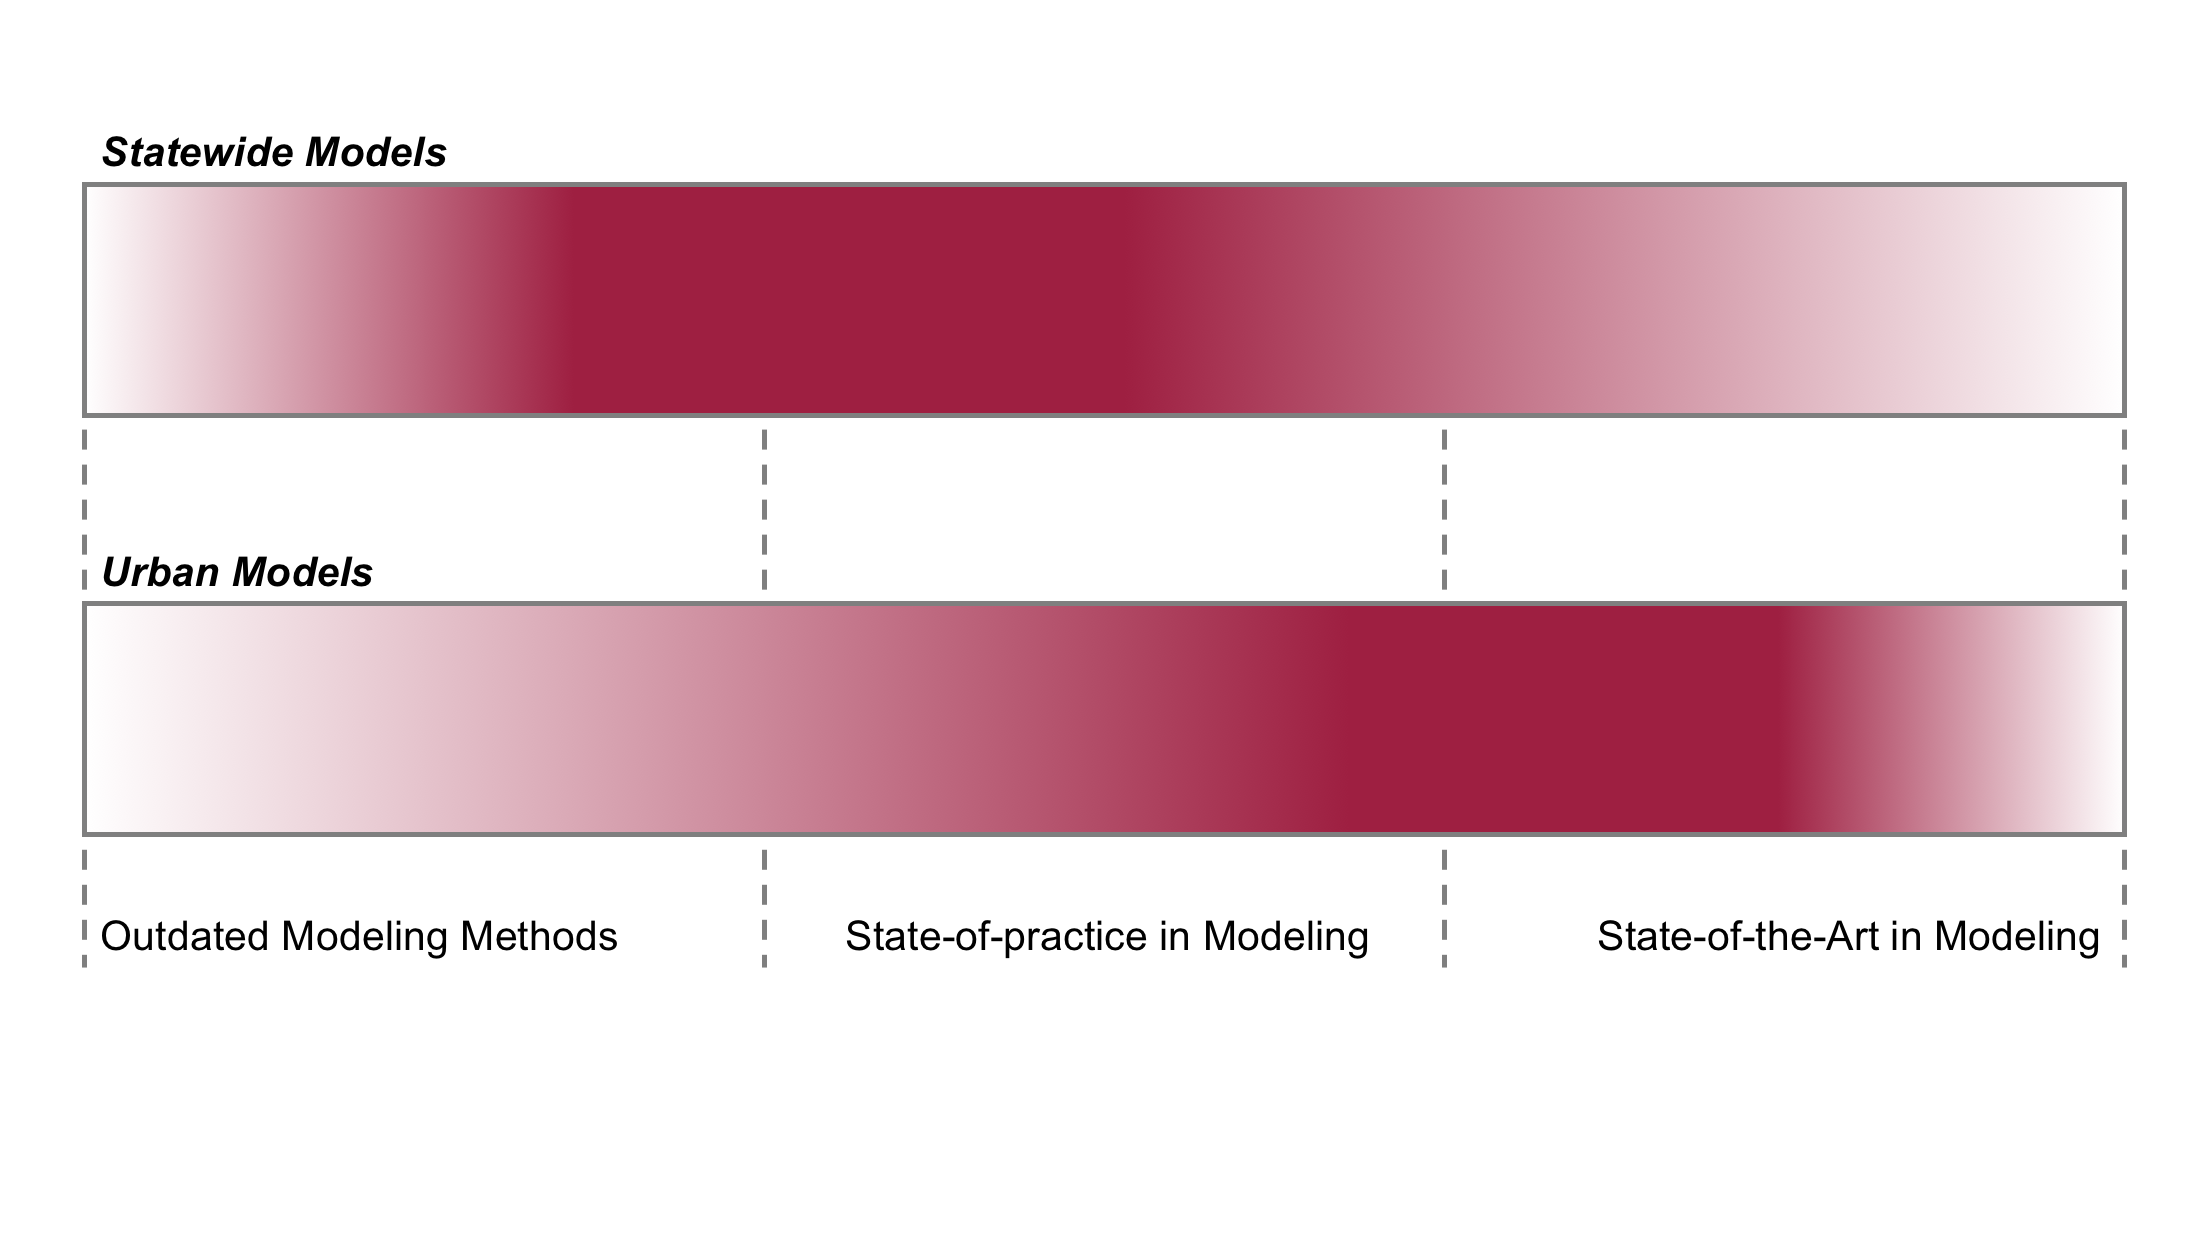
\includegraphics[width=6.4in]{graphics/39-model-development-comparison}
\caption{Attempt to compare level of development of statewide models with urban models}
\label{fig:model-development-comparison}
\end{figure}

However, the fact that statewide models tend to be simpler is not a critique per se. Simpler models may well can answer questions asked in each state. If two models could answer the questions at hand, the simpler model should always be preferred as it limits the risk of model inconsistencies. As Albert Einstein is said to have noted, ``a model should be as simple as possible, yet no simpler.'' Moreover, the temporal, spatial, and behavioral resolutions found in many state-of-the-art urban models would be prohibitively costly if extended to cover an entire state. It appears that most model developers have attempted to balance the desire for greater capabilities with pragmatic concerns about computational and data burdens associated with such models.

Efforts to integrate several statewide models with analytics from other related domains are particularly worthy of praise. Fifteen states operate separate models for person long-distance travel; truck travel is represented explicitly in 21 models for short-distance travel and in 26 models for long-distance freight flows. Another 11 states include some form of a freight mode choice model, an inherently complex undertaking. Finally, six states operate their own economic forecasting model, and two have an operational land use model. Statewide models tend to be more advanced than the average urban model in terms of these interdisciplinary modeling approaches.
\chapter{Data requirements for statewide modeling}

Statewide models require many of the same data as those deployed in urban and metropolitan areas, owing in part to the similarities of the underlying models. However, the scale is different, as is the representation of external markets. Many statewide models now include a national coverage of zones, at lower levels of resolution as the distance from the state increases, as well as explicit representation of visitor travelers. These increase the data burden for statewide model developers and users. Fortunately, considerably more data are available for such broader coverage, reducing the cost of building and maintaining statewide models. 

The many types and levels of data required in statewide modeling are discussed in this chapter. The macroeconomic and geographic contexts are discussed in the next two sections, followed by a discussion of the transportation networks represented in such models. This is followed by a discussion of how data on personal travel behavior and choices are collected, from both traditional and newly emerging sources. A similar discussion of traditional and non-traditional freight data sources and opportunities follows it.

\section{Macroeconomic linkages}

Explicit linkages to macroeconomic models are becoming an increasingly important part of state\-wide models. While still rare in metropolitan travel forecasting models, they have a long history in statewide modeling. Michigan was one of the first states to incorporate the REMI model into their process, over 35 years ago. Several other states have used them for an equally long time. \cite{sorratini00} describe how they used both economic forecasts and input-output (IO) coefficients to improve their commodity flow model in Wisconsin. Such models are typically developed independently, and are used in conjunction, rather than tightly integrated, with the travel forecasting models.

Economic models typically fall into one of two categories. The more traditional category includes macroeconomic forecasts that are typically inputted to the statewide model. However, economic impact models are increasingly being used as well, as described in \S\ref{sec:economic-impact-models}. They can be used singly or in combination. Most operate separately from the statewide model, but are included in the statewide modeling system in a few instances.

%\protect\hypertarget{h.av9jpbxyqir7}{}{}

Economic forecasts for broad areas and industry categories are used to generate estimates of future socioeconomic activities within the modeled area. These appear to be done most often at the statewide or sub-state region level, with modelers allocating them further to counties or traffic analysis zones based upon existing zonal employment estimates, land use data, accessibilities, and other measures.

Firms and employment are most often coded to the two-digit NAICS codes \citep{censusbureau16}. Some states use greater detail for dominate industries within the state, and combine those found less frequently. Others aggregate the two-digit NAICS into families of firm type (e.g., service, retail, manufacturing). Those choices of spatial and industry resolution appear to largely hinge upon data availability.

We found that most states (29 out of 46) reported that they used exogenous economic forecasts in their work, or in the case of eight states no forecast at all. The source of these forecasts varies widely, as does the amount of work going into them. Many reported using forecasts created by the state economist or other state agencies charged with developing them. About a 46 percent rely upon third-party forecasts that are customized, at least in part, to the definition of regions and industry sectors used in the statewide model. There may be cases where these third-party forecasts are also used by other state agencies or instead of official state forecasts, although we did not attempt to quantify such cases.

%\protect\hypertarget{h.jsvny4stsszd}{}{}

\section{Spatial coverages}

Statewide models typically employ a wider range of spatial representations than urban models, in part because of the larger area involved. Various types of data used in model development and application are available only at certain levels of geography, which also dictates the level(s) of resolution used in statewide models. Finally, most statewide models now extend well beyond the state borders, usually with decreasing level of detail as the distance from the state increases. It is common to represent the area within the state and a halo around it with traffic analysis zones that aggregate to counties and Census geographies. Outside of the state successively coarser political and Census geographies are used to represent distant markets. FAF regions, described in \S\ref{sec:traditional-freight-data}, are being increasingly used to represent external markets. Many of the models reviewed use multiple levels of geography during implementation, and for communicating results.

Arguably nowhere is the tension between the number of zones and computational burden felt more acutely than in statewide modeling. In smaller states, it might be possible to ``stretch'' the urban models to cover the remainder of the modeled area, with no loss of resolution or precision in the former. However, this is not practical in most cases, for the run time of most models increases geometrically as the number of zones increase. Even on the best hardware available today advanced models with 7,500 or more zones are cumbersome and slow, with formidable resources required for developing and maintaining data that level of geography. Thus, most statewide models aggregate the zone systems used in urban models where they overlap, and add zones in the areas not covered by them.

A definitive best practice for integrating urban and statewide zones remains elusive. In some cases, groups of urban zones are nested within each statewide zone. Equivalency tables are used to transfer information from one zone system to the other if needed. In other cases, processes for defining unique statewide zones are used. The process for conflating different polygon coverages using GIS software is relatively straightforward. This reduces, if not eliminates, the need to keep the boundaries of urban and statewide zones synchronized.

Automated processes for generating zones can be used for those willing to relax the requirement for exactly matching urban zones (or groups thereof). \cite{moeckel15a} described a process for automatically generating grid cells of varying size, depending upon the underlying levels of household and employment density. This was used to create an alternative zone system for the Georgia statewide model that significantly improved the assignment results, based solely upon the new zone system. 

A variant of this gradual rasterization process has been employed in Ontario, where instead of successively dividing a single cell covering the entire state the process starts with grid cells 50 miles (80 kilometers) on each side covering the province. Each cell is successively divided into four smaller cells, until a threshold activity density or minimum zone size is obtained. This precludes huge zones in Ontario's sparsely populated northern areas. Another variant has been implemented for the Munich metropolitan area, where jurisdictional boundaries were respected. Here, gradual raster cells were created and intersected with municipal boundaries. Resulting small slivers of raster cells that were cut by municipal boundaries were merged with other raster cells within the same municipal area to avoid small pieces of raster cells.

The use of microsimulated synthetic households has become standard practice in activity-based travel modeling. They can be used with traditional trip-based models as well, opening new possibilities for either simulating travel between point locations, or for developing new methods for organizing them into polygons (zones) based on homogeneity of household characteristics (e.g., accessibility to certain travel modes, uniform density patterns). The prospect of simulating travel from point locations instead of zones is not as preposterous as it might seem. National models of Germany and Switzerland were implemented in MATSim using this approach \citep{balmer08}.

Modeling travel between point locations will not obviate the need for zones. It will, however, relax the requirement for the latter to be as deliberately designed for compatibility and uniform activity size or land area as traditional models. The provincial model currently under development in Ontario is based on synthetic households and firms, yet still uses at least two different traffic analysis zone systems. The latter are used to represent skim matrices, accessibilities, and centroid connections to macroscopic traffic assignment models. Certain spatial patterns, such as density, accessibility, parking costs and area types are more efficiently displayed and comprehended in aggregate than individually. The tracing of individual flows in microsimulation-based travel models is useful for modelers. However, it seems unlikely the advantages associated with aggregating data for visualization will diminish, at least when communicating modeling outcomes to non-modelers. Thus, ``the tyranny of zones'' \citep{spiekermann99} appears to be with us for the foreseeable future.

\section{Network representations}\label{sec:network-representations}

Abstract representations of the multimodal transportation system are included in statewide models. These include the networks used by each mode of transport represented in the model, for both personal and commercial travel. It also includes intermodal connectors, border crossings, major freight generators, and in most cases, an external network that connects the states to major external markets. These external networks often become highly aggregated, often to only Interstate and federal highways and major rail corridors as the distance from the state increases.

Most states build their internal roadway networks from geodatabases maintained by GIS teams within the agency. Most originated from centerline coverages and roadway geometric data. These are most often linked to Highway Performance Management System (HPMS), traffic monitoring, and other performance monitoring databases used in the agency. The initial development of the network is often an ad hoc exercise, for once built it is typically used for a long time. Such networks are often refined, either in their source data or just in the statewide model, but the lack of funding for large infrastructure projects has reduced the amount of work required to build and maintain a time series of planned network improvements.

Building a roadway network from existing data source seems conceptually simple, yet it was widely reported as the most time-consuming and frustrating part of building the model. Several reasons were cited:

\begin{itemize}
\item
GIS line layer representations do not easily translate to the directional links used in most travel models. Most third-party modeling platforms include utilities for converting line layers to transport networks, but they rely upon an exact and consistent manner of GIS layer coding that is rarely found in practice. The endpoints of many links do not exactly coincide with those of upstream and downstream links, and often allow movements that cannot be made in reality.
\item
Traffic models require link attributes that are not included in DOT roadway inventories, such as capacity, free flow speeds, and permissible lane use (e.g., parking or turn-only lanes).
\item
GIS networks are not navigable, and thus, their connectivity and proper coding of directionality, the number of lanes, and other attributes have never been rigorously checked.
\item
State DOT databases often lack important streets within urban areas, or have different attributes than those coded for the same roadways in urban model networks.
\item
Traffic count data are stored in different systems than geometric data, and require considerable work to combine with the model networks.
\end{itemize}

Correcting these problems, and addressing related issues, was identified as the single largest cause of delay and cost overruns when building statewide models. Maintaining these networks was also cited as a major resource requirement that distracted from efficiently responding to requests for forecasts and analyses.

The amount of work involved in building internal roadway networks has led some states to explore the use of automated conversion of Open Street Map (OSM) data. This process still requires some manual intervention, as some attributes needed in network assignment are missing, and there is no guarantee of network connectivity. Moreover, rural networks are often not as quickly updated as urban ones, which enjoy a larger group of committed users. Thus, while OSM solutions have been applied in research settings (compare \cite{ziemke16} for the state of Maryland), no state appears close to having successfully used it as the officially sanctioned source of internal network data.

Ironically, building the external highway network, as well as networks for other modes of transport, is often much easier. Many states use the National Highway Planning Network developed by USDOT or the Oak Ridge Network, developed for coding and analysis of national freight data sources, for this task. They are already coded in the format required for travel forecasting, although lack the level of detail required within the target state. The National Rail Network is likewise often used, sometimes in conjunction with more detailed network data from Railinc. Pipelines are often omitted, and marine and air networks and ports are small enough that they are easy to code using federal data sources.

A gray area in the middle is the representation of public transit. Fixed guideway transit systems are relatively easy to code, for both urban and intercity systems. Except for the Northeast and West Coast, the intercity public transportation networks are relatively sparse. Federal sources of network data are lacking, but these can typically be coded from metropolitan and carrier-provided network data. General Transit Feed Specification (GTFS) data are now routinely used by some agencies to automate the coding of fixed guideway transit networks and their service characteristics.

A thornier aspect involves how local bus transit services are included in statewide models. While they can now be coded much faster and more accurately using GTFS, their addition to statewide models remains problematic. The larger zones and coarser urban travel market segments make the coding of access and egress more difficult and less accurate, and the need to include local streets that buses run on can greatly increase the number of links required in the model. This, in turn, imposes an additional computational burden, especially for path-building in highway and transit assignment. Thus, even if GTFS could automate what would otherwise be a hugely onerous network coding task, would the results be worth the effort? Two different approaches have emerged that offer a tractable alternative:

\begin{itemize}
\item
\cite{circella13} developed a process for building an abstract representation of likely local bus accessibility, based upon urban form characteristics. The approach was initially developed in Oregon, and later improved during its implementation in California. Zone-to-zone bus travel times are calculated as a function of auto interzonal travel times. Assumptions about fares and service levels must still be made by the user, but robust bus travel times can be estimated using the coarser networks typically found in statewide models.
\item
Logit averaging can be used to represent composite impedances and accessibilities from urban models, where bus transit is modeled explicitly, to statewide models. This obviates the need for network coding, as the mode choice logsums are computed on a zone-to-zone basis, but are not influenced by how the zones are designed. This approach is being used in HSR forecasting in Texas.
\end{itemize}

Both approaches offer tractable and affordable alternatives to maintaining extensive local transit networks, which typically only play a small role in intercity and major statewide flows.

\section{Traditional personal travel behavior data}\label{sec:traditional-person}

Statewide models typically include a wider range of diverse travel markets than traditional urban models do, increasing their data requirements for model development and application. Visitor travel, for example, is often explicitly represented within statewide models at varying levels of fidelity and resolution. Moreover, statewide models must accommodate the diversity of travel behavior and choices by residents living in metropolitan, suburban, small towns, and rural areas. Merely enumerating these markets can be challenging in some cases, much less the collection of data about them, and accommodating such within a single modeling framework.

The behavioral data used in statewide models came primarily from four sources, as shown in Figure \ref{fig:behavioral-data-sources}. The NHTS was used by almost two-thirds of the states that reported what type of behavioral data they used in building and applying models. Household travel surveys were used by almost half of the states, while synthetic and transferable rates compiled in various NCHRP reports were used almost as frequently. Passively collected data, described in the next section, was reportedly used by a quarter of the states.

\begin{figure}   % 40
\centering
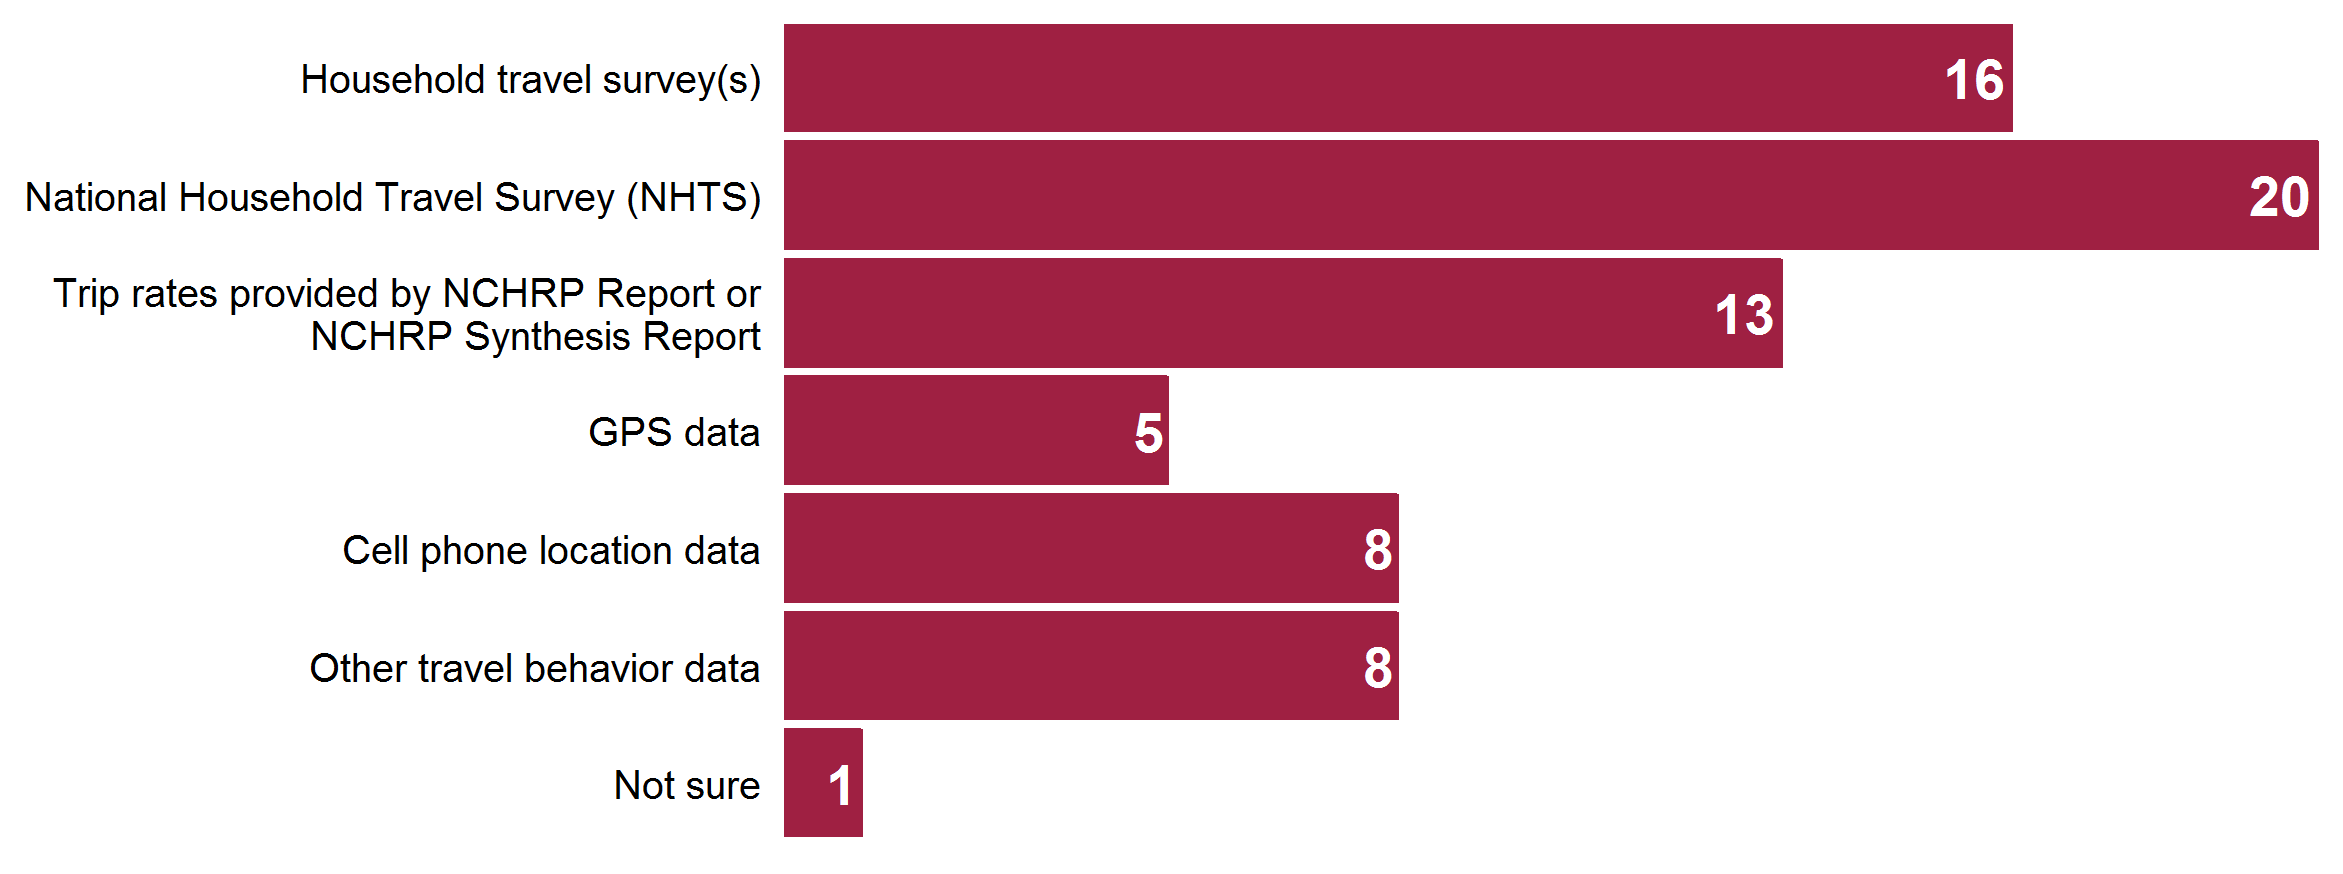
\includegraphics[width=6.4in]{graphics/40-behavioral-data-sources}
\caption{Behavioral data sources used for building statewide models}
\label{fig:behavioral-data-sources}
\end{figure}

Most states reported using multiple data sources. However, the ways these data were combined reveal almost no pattern of standard practice, as shown in Table \ref{tab:data-combinations}. The exclusive use of the NHTS by a quarter of the states is surprising, and indicates its importance in statewide modeling. Five states reported using only household travel surveys for model development, which is also surprising, given the additional markets covered in most statewide models that such surveys do not illuminate (e.g., visitors, long-distance travel). However, four of them --- California, Michigan, Ohio, and Oregon --- conducted statewide surveys that provided data for all households across the state, reducing or obviating their need to supplement their survey data. The characteristics of the surveys conducted by these four states are summarized in Table \ref{tab:comprehensive-surveys}.

\begin{table}   % 3
\centering
\caption{Combinations of data used to build statewide models}
\label{tab:data-combinations}
\begin{tabular}{lrr}
\hline
Data source(s) used & n (states) & Percent \\
\hline
National Household Travel Survey (NHTS) & 7 & 24.1 \\
\gray Household travel survey (HTS) & 5 & 17.2 \\
HTS and NCHRP rates & 2 & 6.9 \\
\gray HTS and passive data & 2 & 6.9 \\
HTS and NHTS & 2 & 6.9 \\
\gray HTS, NHTS, and NCHRP rates & 2 & 6.9 \\
NHTS and NCHRP rates & 2 & 6.9 \\
\gray NHTS and passive data & 2 & 6.9 \\
NHTS, NCHRP rates, and passive data & 2 & 6.9 \\
\gray NCHRP rates and passive data & 2 & 6.9 \\
NCHRP rates & 1 & 3.4 \\
\hline
Total & 29 & 99.9 \\
\hline
\end{tabular}
\end{table}

\begin{table}
\centering
\caption{Comprehensive statewide travel surveys}
\label{tab:comprehensive-surveys}
\begin{threeparttable}
\begin{tabular}{llclrr}
\hline
State & Survey & Year(s) & Survey Type\tnote{a} & Households & Cost\tnote{b} \\
\hline
Ohio & Household Travel Survey & 2003 & 24-hour HTS & 15,000 & \$2.0M \\
\gray Ohio & Long Distance Travel Survey & 2003 & 2 week RTS & 8,000 & \$0.4M \\
Michigan & MI Travel Counts I & 2004-05 & 48-hour HTS & 14,966 & \$2.1M \\
\gray Michigan & MI Travel Counts II & 2009 & 24-hour HTS & 1,975 & \$0.52M\tnote{c} \\
Oregon & Oregon Travel and Activity Survey & 2009-11 & 24-hour HTS & 18,282 & \$3.6M \\
\gray California & California Household Travel Survey & 2012-13 & 48-hour HTS & 42,431 & \$10M\tnote{d} \\
California & California Household Travel Survey & 2012-13 & 2 month RTS & 18,012 &  \\
\gray Michigan & MI Travel Counts III & 2015 & 24-hour HTS & 16,276 & \$2.4M \\
\hline
\end{tabular}
\begin{tablenotes}
\footnotesize
\item[a] HTS = household travel survey, RTS = retrospective (long-distance) travel survey
\item[b] Current dollars in the year the survey was contracted
\item[c] Higher cost attributable to inclusion of an attitudes and perceptions add-on survey
\item[d] Cost shown includes both household and retrospective survey
\end{tablenotes}
\end{threeparttable}
\end{table}

The four statewide surveys are notable in their scope, covering the entire state. They also featured large sample sizes and use of common sampling approach and instruments across the state. Most were stratified to obtain usable sample sizes for different areas of the state or area type (e.g., metropolitan, small urban, rural) in addition to the usual stratification by household attributes. The findings typically reveal different travel patterns by sub-state areas. In Oregon, for example, rural residents make fewer but longer trips, with more intermediate stops than urban residents. Applying urban patterns to the remainder of the state would result in significant errors or incorrect policy sensitivities. Thus, these large-scale surveys are a sound investment. Moreover, collaboration with the MPOs within each state results in a common approach to conducting such surveys, enabling each to obtain a large sample of usable observations than either could afford alone.

Not shown in Table \ref{tab:comprehensive-surveys} is a new statewide survey getting underway in Ohio as this report was being finalized. They are planning to spend approximately \$7.5 million over the next decade to collect data from 2,500 households per year. Their target is to obtain seven days of data collection for each household, with 70 percent including GPS collection on smart phones. Most notable about their effort is highly rigorous ``zero defect'' requirements for survey completion. Their goal is to eliminate incomplete responses and missing data from certain household members, which if successful will advance the state of practice for all household travel surveys, not just at the statewide level.

Several other states used metropolitan travel surveys, often in combination with other data sources, to build statewide models. In Maryland, for example, urban household travel surveys conducted in different years by the Baltimore Metropolitan Council and the Metropolitan Washington Council of Governments were fused to develop the statewide model. The former had enough samples from suburban counties to help differentiate their differences in travel behavior. However, the biggest differences were in the travel patterns of residents of the two major cities, underscoring the importance of accounting for the unique characteristics of different urban areas within statewide models.

As useful as the statewide travel surveys are, they typically only gather information about daily travel patterns on the survey day(s). They are less useful for understanding certain aspects of travel behavior important in statewide models:
\begin{itemize}
\item Their sample sizes are too small to reveal robust origin-destination patterns
\item Long-distance trips are under-represented
\item Visitor trips are not captured
\end{itemize}

It is widely accepted that household travel surveys are large enough to illuminate differences in trip and tour formation and structure \citep{stopher07}, but too small to reveal origin-destination patterns unique to the surveyed area. Census journey-to-work data at the county level have long been used to better understand commuting flows in statewide models, but are limited to information about that trip purpose, with frequent suppression of smaller interchanges that collectively prove important in understanding flows between urban areas. This is an area, however, where big data are being used to fill that long-standing gap in knowledge. Such opportunities are described in the next section.

Long-distance travel, which takes place less frequently, is rarely captured in household travel surveys in large enough numbers to be useful. Only Ohio and California have administered separate long-distance travel surveys. It is widely acknowledged that two to three-month retrospective surveys are more useful for collecting information about these types of infrequent trips. Unfortunately, there are little national data to borrow from to construct such models. While used extensively in Europe, the last large-scale long-distance travel survey in the USA, the American Traveler Survey, was conducted in 1995. The small long-distance add-ons to the National Household Travel Survey (NHTS), conducted in 2001-02 and 2009, are considered too small to be very useful. This has not stopped modelers from attempting to use them despite their small size, although results have been uneven at best.

The largest time series of long-distance travel data in North America are the Travel Survey of Residents of Canada (TSRC) and International Travel Survey (ITS), both conducted by Statistics Canada. Since its last overhaul in 2010, the TSRC has continuously collected data on long-distance travel, which are available to researchers as microdata. The data are being used to develop provincial travel models in Ontario and Alberta, using different methods in each. They are being used to develop microsimulations of resident and visitor long-distance travel by season in Ontario, whereas model design is just getting underway in Alberta.

The national scope of the TSRC and ITS enable them to be used to build models of both resident and visitor flows. While a work in progress at this writing, preliminary results show important differences in the characteristics and travel patterns in residents of versus visitors to Ontario. The transferability of these models to the USA is an open question. However, the Canadian program provides an encouraging example of a well-run survey that is almost singular in its scope and breadth, as well as utility for building robust statewide models.

The published syntheses of travel data from several NCHRP reports were widely used in building statewide models. These include:
\begin{itemize}
\item NCHRP Report 716, ``Travel demand forecasting: parameters and techniques'' \citep{cambridge12}
\item NCHRP Report 735, ``Long-distance and rural travel transferable parameters for statewide travel forecasting models'' \citep{schiffer12}
\item NCHRP Report 765, ``Analytical travel forecasting approaches for project-level planning and design'' \citep{cdmsmith14}
\end{itemize}

The way in which these reports were used was interesting. Follow-up conversations with respondents who indicated they exclusively used the NCHRP reports did so because funding limitations precluded primary data collection. The states that used the reports in combination with other data sources, by contrast, primarily used them to glean information about the unique travel patterns of rural residents, develop model calibration and validation targets, and assess the reasonability of delivered models.

Some states employed roadside interviews of motorists in the past, attempting to overcome the paucity of data on long-distance travel. They also used such data to focus on key corridors across the state. Our findings suggest that this practice has largely been abandoned. Interviews had to be completed quickly if done on site, limiting the amount of information collected. Mail-back surveys enabled more data to be collected, but suffered from low response rates. Even where the data were collected on-site the surveys suffered from small sample sizes, inability to control for non-respondent bias, high cost per completed interview, and questionable transferability, even of aggregate summary statistics. However, it appears that legislative or executive prohibitions on the practice, prompted by citizen complaints, effectively ended roadside interviews in most states rather than methodological or data quality considerations.

\section{Non-traditional personal travel behavior data}\label{sec:nontraditional-person}

The growth of big data solutions for transport planning applications has arguably had no greater early successes than in statewide modeling. These data are passively and continually collected from cellular and GPS devices, and summarized in origin-destination and travel time matrices and summaries by third parties. Almost a quarter of the respondents who revealed their sources of data reported using AirSage data for model development. These data can fill the gaps in knowledge noted earlier about infrequent long-distance travel, as well as revealing origin-destination patterns within the modeled area. It is important to note that the AirSage data do not represent the universe of big data solutions, and arguably might not be the biggest player in that rapidly expanding market. However, they were the most frequently cited vendor. The experiences reported provide useful insights that will likely apply to many big data products used in statewide modeling.

Some details of how AirSage collects and processes data are proprietary. What is known, however, is that they receive a time-stamped position record every time a transaction with a Verizon or Sprint device occurs. Some users rarely use their mobile phones, but most have a variety of applications always active, ensuring a constant stream of location coordinates from a customer base that is estimated at half the cellular phone market in the USA. Given that mobile phones are almost ubiquitous this equates to a continual stream of travel tracking data from about half of the population, over several years. Simple heuristics can be applied to the raw data to identify the likely home and work or school locations, based on when, how often, and how long they repetitively visit certain locations.

It does not appear that AirSage attempts to fuse their data with business location, household, or land use information to further infer what activity the traveler is engaged in during each stop. Nor is it clear how they identify (activity) stop locations in the first place. However, with few exceptions their ability to differentiate home-based work, home-based other, and non-home-based trips should be robust, especially at the level of spatial resolution in most statewide models. Some users have questioned the validity of the data at fine levels of geographic resolution, or ability to use it for constructing tour-based models (where identification of intermediate stops is important). However, these are likely to be outside of the interests of most statewide modelers. Moreover, the broader levels of spatial resolution and trip purposes do not distract from the value of the data for model validation or reasonability checking.

Because the typical home location of the otherwise anonymous user is known it is easy to know when they travel outside of their normal area, or to pinpoint long-distance commuters. This enables AirSage to create a visitor trip matrix for any given study area, to include information such as where visitors spend the night, clusters of activity locations during the day, and visit duration (time away from normal area). The value of such data for modeling visitors in statewide models cannot be understated.

Several other vendors have entered the big data market, including INRIX and StreetLight. They use alternative sources of information or add data and value to the raw AirSage data. Both can provide data on internal travel times, or at least for larger origin-destination flows, which AirSage does not. Even though these big data sources lack characteristics of the traveler (other than what can be inferred from where they live and work) and the trip, they remain invaluable for statewide modeling. Reliable and robust OD patterns for both residents and visitors can be constructed from these data, whose sample size is at least two orders of magnitude larger than any known household travel survey. The latter cannot provide reliable OD patterns except at very coarse geographic levels, while the former can easily work at the level of the coarse zones typically used in statewide models.

It must be acknowledged that cellular tracking data are less than ideal on their own. They include no information about the trip or trip-maker, with whom they travel and why, or mode of transport. The latter can be inferred when only a single mode is available or practical, or when certain speeds are reached. However, such analyses would require access to the raw data and considerable additional analyses, which are not available to modelers. Thus, they have become indispensable for statewide modeling, but only when fused with the traditional data described in the previous section. Several innovative uses of these data were reported at the TRB Innovations in Travel Modeling 2016 conference, but have not made their way into the literature at this writing.

\section{Traditional freight travel data}\label{sec:traditional-freight-data}

Understanding long-distance freight movements is often as important in statewide modeling as depicting personal travel. Interstate trucking is often a high percentage of flows on Interstate highways, and exerts a disproportionately high impact on them. There is a long history of modeling inter-regional commodity flows within the USA, some of it quite sophisticated even by today's standards. However, data on freight flows, especially for trucking, have historically been elusive, especially at the level of geography used in statewide models. Most of the data are from federal sources, and are aggregated to large sub-state or statewide regions before release.

While the Commodity Flow Survey (CFS) provided a long time-series of information about domestic flows from shippers in certain industry categories, the data were only available in summary tables until 2015. Many flows were masked due to confidentiality requirements or concerns about sampling errors, making the construction of OD matrices by mode of transport and commodity group difficult, if it could be done at all. The flows were measured in annual dollars (of commodity value) and tons, rather than the weekly or daily vehicle flows by mode needed by modelers.

A variety of approaches were tried over the years to translate annual commodity flows into estimates of traffic by mode, with varying degrees of success. Most gravitated towards a fusion of employment, economic input-output, CFS, and truck count data first proposed by \citep{polenske74, polenske75}. Variants on her approach, as well as means of allocating the flows from counties to statewide model zones, were implemented in several states in the 1980s and 1990s, mostly in the Upper Midwest. Michigan and Wisconsin have tried several approaches over the past forty years. They all required custom code and a wealth of borrowed data fused in an ad hoc manner.

All of that changed with the introduction of the Freight Analysis Framework (FAF), originally developed by FHWA in 1997-99 as a tool for federal policy analyses. It has undergone three significant revisions since, with the first release of Version 4 in 2014. The initial version was a proof of concept, which has undergone significant enhancements in the intervening years. The CFS is the backbone of the FAF, and each major update has coincided with the release of the latest version of the CFS. However, considerable value is added to the data by fusing them with other data, to include the Carload Waybill Sample rail data, domestic and international waterborne commerce data, air freight data compiled by the USDOT, foreign trade statistics, and the Vehicle Inventory and Use Survey (discontinued by the Census Bureau after release of the 2002 survey data).

Unlike the CFS, recent versions of the FAF provide a comprehensive database of freight flows rather than limited static tabulations. Two principal databases are produced:
\begin{itemize}
\item
Origin-destination flows of freight by commodity and mode of transport, measured in tons, value, and ton-miles. These are provided at the county level or international gateway for users within the USDOT, and at the level of FAF regions or international gateway markets for all other users.
\item
Estimates of flows on major routes and segments of highways, by mode of transportation. A range of tonnage is provided at the route level, while truckload equivalents and tons of truck-carried freight are available for segments. Additional attributes are available to USDOT users, such as the commodity and origin-destination data.
\end{itemize}

The FAF is not so much an analytical framework --- a phrase that suggests underlying models --- as it is a commodity flow database. There are no user-accessible analytical methods or products embedded within the FAF. No mode choice model is included, nor are any other policy-sensitive models. Consequently, existing patterns and trends are extrapolated into the future. This can hardly be construed in a negative light, considering that existing choices and preferences remain invariant in most travel demand forecasts. Moreover, the amount of progress made over the past several years is remarkable nonetheless. Perhaps most importantly, the FAF can be used with statewide or national freight models in a far easier manner than the CFS alone.

FAF Version 4 data are available for its base year of 2012, and forecasts in five-year intervals from 2015 through 2045. The forecasts are based upon an exogenous forecast by region in the USA compiled by IHS Global Insight and assumptions about changes in markets and technologies over the forecast period. The economic forecast in Version 4 was widely welcomed, as it was the first FAF forecast to incorporate the effect of the 2008-09 economic downturn and subsequent recession. All modes of freight transport are included in the FAF. Like the CFS, commodities are classified using the Standard Classification of Transported Goods (SCTG) system \citep{bts15}.

The FAF is not without its limitations. Several modelers cited its questionable accuracy, especially when the inter-regional flows are translated into truckload equivalents. Some states report that the data appear quite reasonable, and match heavy truck counts on their borders within acceptable margins. Others report much wider errors. Another lingering and often cited limitation of the FAF is its coarse level of spatial resolution. The data are available at the county level for internal use within the USDOT. However, they are substantially more aggregated when released to all other users, who can only obtain information at a much coarser geographic scale. The 132 FAF regions within the USA nest within states, and counties nest within FAF regions. While the data are still more aggregate in nature than many state and local planners need, it represents a significant improvement over the CFS. Several major metropolitan areas are included in the regions, allowing flows affecting these areas to be more accurately represented.

The FAF is an excellent and important data source for statewide models despite these limitations. Its availability has fundamentally changed the way most states approach freight modeling. Some still rely upon bespoke models or third-party data, but most use the FAF today. Its transparency, greater level of detail, availability of forecasts, and online documentation make it easy to incorporate into statewide models. Several techniques have been developed to disaggregate flows between FAF regions to flows between counties, or even between statewide model zones. The methodologies have traditionally been developed on a case-by-case basis, and are rarely published. Most approaches use one of two procedures, singly or in combination:

\begin{itemize}
\item
Multiple Regression: Commodity-specific flows into and out of a FAF region are used as the dependent variable and employment by type are used as the independent variable. Linear multiple regressions are used to estimate parameters that help explain which employment types generate and attract flows of a given commodity. These parameters are used to disaggregate to smaller zones within a FAF region.
\item
Input-Output Coefficients: Such coefficients describe which commodities are consumed and produced by a given industry. Multiplying employment by type with the corresponding IO coefficients generates a weight for every region that can be used to disaggregate FAF flows.
\end{itemize}

Both methodologies have been applied widely and appear to generate comparable results, at least at the level of the assignment. The former approach has the limitation that parameters are estimated based on large FAF regions with a homogeneous industry mix across the country. The latter approach relies on input-output coefficients that commonly are estimated as dollar flows, while freight flows usually are processed as weight-based flows.

Like the CFS, the FAF expresses freight flows in annual value and tonnage terms. \cite{battelle12} developed a framework for estimating truckload equivalents of the OD flows by tonnage, to include imputation of empty vehicle backhauls, which appears to be used to generate weekly or daily truck flow estimates.

The proprietary Transearch database of commodity flows is similar in structure and coverage to the FAF. It was originally developed by Reebie Associates, but was acquired by IHS Global Insight in 2005. They have continued to offer the same product, as well as bundle it with other consulting services and data subscriptions. Earlier versions of the Transearch database were thought to be based upon the CFS, and supplemented with staff interpretation, addition of additional data from private and third-party data, and surveys conducted by Reebie Associates. Then, as now, the methods used to develop and test the Transearch data are not divulged, nor is information about what the forecast series are tied to. It seems likely that they are tied to IHS Global Insight forecasts, given their present ownership.

The Transearch data have traditionally been offered at a finer level of geographical detail than either the CFS or FAF. The definition of geographical coverages is flexible, and appears to be specified by each client. Within the area of interest, the data are typically provided at the county level and aggregated to approximately 400 Bureau of Economic Analysis (BEA) economic areas, states, or multi-state Census regions outside of it. The ability to customize the level of geographic resolution is an important value added to the Transearch data, even if IHS uses the same methods described above for synthetically allocating FAF data to counties.

Commodities are classified using the Standard Transportation Commodity Codes (STCC), which was used in the CFS before 1997 and is still used by the railroads and in the Carload Waybill Sample. The advantages of the Transearch data include its flexible level of geographic representation, vendor support of the product, and its claimed addition of other data sources to improve the estimates. However, its cost and lack of transparency reduce its utility in model development. Ideally, both data sources could be used to develop statewide freight models, for understanding the differences between the two data products may in some cases be more revealing than singular estimates from either.

\section{Non-traditional freight travel data}\label{sec:nontraditional-freight}

Big data are fundamentally changing our understanding of freight flows, in much the same way they are revolutionizing the analysis and modeling of personal travel. Data about trucking flows and patterns have traditionally been the most difficult and costly to obtain, despite its dominance in freight transport and impact upon roadway infrastructure, road safety, and emissions. 

The introduction of GPS truck tracking data from the American Trucking Research Institute (ATRI) in 2012 has significantly helped to fill that knowledge gap. Like the AirSage data, continuously collected time-stamped coordinates for uniquely identified but anonymous trucks are available. The truck type is unknown, as is the cargo it carries. However, its complete itinerary can be viewed over any desired period. Considerable post-processing is still required to translate the GPS coordinates, and the distance and travel time between them, into stops by duration. Personal travel is typically habitual, limited in the area covered, and occurring within certain hours of the day. Truck travel looks almost random by comparison in many cases, complicating the delineation of tours and stops \citep{sharman11}.

Despite the challenges involved in teasing out discrete tours and stops the ATRI data have been used extensively in statewide models. The use of the data in OD matrix estimation of statewide truck flows has been widely reported in the literature over the past two years. Most use the ATRI data to construct the seed matrix required for the process, requiring the analyst to reduce the data to tours and stops. Many researchers have adopted a rule to define stops based upon the time remains stationary at a given point. Five minutes has frequently been used as a threshold to define a deliberate stop (i.e., to pick up or deliver goods and services, driver breaks, or vehicle maintenance), which seems reasonable for analysis of intercity truck tours. It seems unlikely that a significant amount of cargo could be loaded or delivered in less time.

\cite{bernardin14} describe how they employed this process in Tennessee, with many similar reports appearing in recent literature and conferences. One of the more comprehensive reports, with a detailed description of the tour and stop synthesis process, is a similar report on applications in Florida by \cite{pinjari14}. At least six similar applications have been reported in the literature and at recent conferences. All point to the utility of using these data to describe truck movements across the state, as well as connections to the markets it serves. The fusion of FAF and ATRI data has yet to be reported, but is known to be under development by several researchers.

Other vendors are beginning to offer products for commercial vehicles as well. StreetLight offers data commercial vehicle flows, generated using INRIX data and possibly other sources. Several fleet management systems offer GPS tracking, but have not yet marketed their data for transportation planning purposes. However, the capability to collect and process these data are becoming more ubiquitous, which will likely facilitate more vendors offering comparable products.
\chapter{New and emerging methods and opportunities}\label{sec:emerging-methods-opportunities}

Statewide modeling is on the brink of a dramatic revolution. It has gone from being employed in only a few dozen states a decade or two ago to use in almost all states. They are being used to inform a wide variety of policy and investment decisions, and are becoming more mainstream in statewide and regional planning processes. The experience gained with a wide variety of approaches, and varying degrees of resolution and sophistication, is slowly resulting in a standard practice of statewide modeling. However, there are several important methodological and technical trends that are quietly reshaping how statewide models are built and used, as well as how they evolve and are used to communicate results to a wider audience than modelers:

\begin{itemize}
\item Vastly expanded use of big data to build networks, trip matrices, and eventually, travel diaries for both personal and commercial travel
\item Incorporation of national data and models in place of current long-distance travel models, particularly for visitors
\item The potential for using networks and time series of travel times from person and commercial vehicle navigation system
\end{itemize}

These influential trends are described in this chapter. Some are mature enough for immediate implementation, while others are emerging Individually they can substantially improve statewide models at a reasonable cost, but even more so collectively. How big data might be used to develop and maintain statewide models are discussed next, followed by a discussion about how national models might usefully inform statewide models and reduce the amount of work required to represent external and national markets. Strategic visioning models might also have a place in statewide modeling, either alone or in combination with more traditional approaches, as discussed next. The potential for using the same networks used in personal and in-vehicle navigation systems are discussed next. The chapter closes with a brief discussion about how states might jointly develop and maintain models, reducing the cost to each.

\section{The potential of big data}

Transportation planners have high expectations about the utility for and low cost of big data in all aspects of their work. Statewide modelers have the same expectations, and have already begun to use them in several cases, as described in \S\ref{sec:nontraditional-person} (for person travel models) and \S\ref{sec:nontraditional-freight} (for freight applications). These data can provide information about infrequent long-distance trips by residents of the study area, as well as detailed data about the travel patterns of visitors within it. At present these data are normally supplied in traditional trip matrices for person travel, with rather coarse trip purpose definitions, and their more successful uses appear to be with larger zone sizes. Some vendors offer similarly aggregated travel time information. By themselves, these data only inform us about past travel patterns, but provide no insight into the characteristics of the traveler or trip, or their interactions. They also provide no insight into how trips are structured into tours to meet the full travel needs of an individual or household.

Many believe that this represents the first successful use of big data in travel demand modeling. They are correct about the sheer volume of data, for just storing a few years of the raw cellular tracking data used to build these data for a single state or metropolitan area requires petabytes of data storage. Mining these data requires formidable computing resources and talent, which none of the states have developed or revealed plans to. However, the USDOT has already invested in big data compared to the traditional practice of travel demand modeling over the past few decades. The NHTS represents a significant national resource, even if its sample size in any one given metropolitan area or state precludes it from being used alone to build robust models. The CFS and FAF, discussed in \S\ref{sec:traditional-freight-data}, were not designed as big data programs, but arguably have become so.

As noted, these data can immediately be used to build trip matrices that can be used as calibration and validation targets for trip distribution or destination choice models. The behavioral insights offered through estimation of destination choice models, for example, provide insight into the variables most influential in traveler decision-making. However, the household travel surveys used to develop such models lack enough observations to enable the analyst to ensure that the spatial patterns of destinations chosen, which are unique for each modeled area, are replicated to an acceptable degree. We have a lot to learn about how to combine small household travel surveys with data from tracking half of the population through time and space within the modeled area, but the resulting models will be remarkably more robust than those employed today. Several states, including North Carolina and Ontario (Canada) are known to be experimenting with such techniques.

The vast potential for third-party and government big data programs will emerge when methods for fusing them mature. The raw GPS tracking data can be associated with surrounding land use information at stop locations, and perhaps focused analyses of large clusters of activities. More powerful would be analyses of patterns of joint or similar travel behaviors. However, such matching will likely always be ambiguous except in cases of stops at isolated facilities, or large campuses (e.g., schools and universities, medical centers, factories).

A more expansive approach is to fuse both actively and passively collected data using new methods. \cite{kressner16} created tour patterns for medium-sized communities from fusing the tour patterns found in the NHTS with AirSage origin-destination matrices, using discrete event simulation (DES). The resulting tours from the prototype model replicated observed flows on the Asheville, NC network as well as a well-calibrated trip-based model. This type of DES has not previously been used in travel demand forecasting. However, it has been widely used in other domains to replicate individuals and systems using data collected at varying levels of spatial, temporal, and behavioral resolution. Such models often use a variety of modeling approaches within each modeling system, to include deterministic and stochastic models, sampling from observed or asserted distributions, rule-based methods, and evolutionary models. Artificial intelligence approaches, such as neural networks, might also be employed. The point is that several alternatives to deterministic discrete choice models based on econometric estimation abound, many of which are much better suited for DES and other approaches to fusing, mining, and forecasting with big data.

\section{Integration with national models}\label{sec:national-model-integration}

Statewide modelers a generation ago were faced not only with the challenge of building models capable of capturing the diversity of travel within their state, but to also account for trade and travel with others states and through trips (i.e., trips with both ends outside of the modeled area). In some cases, flows on Interstate highways in adjacent states affect those within the modeled area, but little is known about who travels on them or why. The auto industry in Michigan, for example, had supply chain linkages all over the continent, with different mode choice possibilities depending upon the commodity and distance traveled to or from the state. Their statewide modelers were faced with the need to represent external markets (outside the state), as well as estimating flows to and from them. Commodity flow models were often developed using the CFS, often duplicating the work in nearby states, or expending considerable efforts of their own.

The FAF changed that, such that many states now use the FAF or Transearch data (described in \S\ref{sec:traditional-freight-data}) in conjunction with a scaled-back version of a national network, such as the Oak Ridge Network. Such models can be developed quickly, and in a consistent manner, from well-documented public data. It lacks the level of geographic detail required for most statewide models, but a wide variety of techniques exist for imputing more detailed origins and destinations. As noted earlier, the ATRI truck GPS tracking data are already being widely used for synthesizing long-distance truck origins and destinations at the statewide model zone system. This practice will become the norm in statewide modeling, if not already so in many states. Moreover, the GPS tracking data can be used to check and adjust the FAF flows for individual states in ways that are not yet available at the national level.

One criticism of the FAF is that it is an inventory of existing flows, with static (policy-in\-sen\-si\-tive) forecasts for future years. This limitation is being addressed through the development of a be\-hav\-iorally-based national freight demand model. It is currently under development by FHWA, and expected to include explicit models of freight generation, destination, and mode choice within a supply chain perspective, as well as truck tour formation and routing heuristics. The model is based on a newly proposed national use model areas (NUMA), consisting of counties across the country and further disaggregated into Public Use Microdata Areas (PUMA) within the more populous ones. This will provide at least an order of magnitude more geographic specificity than the FAF data. Combined with truck GPS data to illuminate clusters of truck activities within each zone, this national model will surpass the capabilities of almost all statewide freight models in existence. This will enable states to "plug-and-play" with the national model, reducing the cost and development time associated with building customized models for each state. The funding formerly associated with the latter can presumably be pooled to improve the extent and quality of data used in the national model, enabling it to improve in quality as it evolves, much as the FAF has done.

A similar framework has been proposed for a national long-distance person travel model \citep{outwater14}. The proposed modeling system consists of a tour-based microsimulation of annual long-distance person trips for all travel purposes and modes of transportation. It is conceptually more sophisticated than a similar simulation developed by \cite{moeckel11}, which only replicates existing patterns. The design proposed in this research includes activity participation and scheduling, time use, and joint mode and destination choice models at the level of the same 4,570 NUMAs proposed for the national freight model. A proof of concept was developed, although as research conducted under USDOT's Exploratory Advanced Research program rather than as an ongoing federal effort. It will require major new data collection on long-distance travel on a national scale to succeed. These requirements are well beyond the data available from the long-distance NHTS described in \S\ref{sec:traditional-person}, even if supplemented with similar surveys from states that have conducted them recently, such as California and Ohio. It is presumed that the long-distance element of the more recent California Household Travel Survey would be included as well.

The development and maintenance of a statewide model would be considerably simplified by incorporating these two national models. Ideally, both would be based upon the same NUMAs and national network, and use consistent land use, socioeconomic, and transportation system assumptions and data. There are several challenges associated with such an approach, to include the interface between the more detailed statewide geographic and network coverages used at the statewide level. The precision and accuracy of the national models, how the national models would be run within the statewide model, and data interchange between the different modeling systems are also important issues. It is assumed that these integration issues, similar in many ways to the issue of statewide-urban model integration, are details that can be overcome. It remains an open question whether USDOT, or perhaps a coalition of states, will support these national models.

A conceptual view of such an integrated modeling system is shown in Figure \ref{fig:integrated-opportunities}. National multimodal forecasts of long-distance travel can be published for forecast years, in much the same way the FAF is disseminated. In an ideal configuration, the states could make custom runs of the national model, to explore how changes in assumptions about socioeconomic and transportation system growth might affect long-distance travel patterns. In either case, the data can be accepted by the statewide model, and allocated to finer temporal and geographic representations if required. The data used to build and apply the national models could also be accessed directly by statewide modelers.

\begin{figure}[!t]   % 41
\centering
% Change scale when found
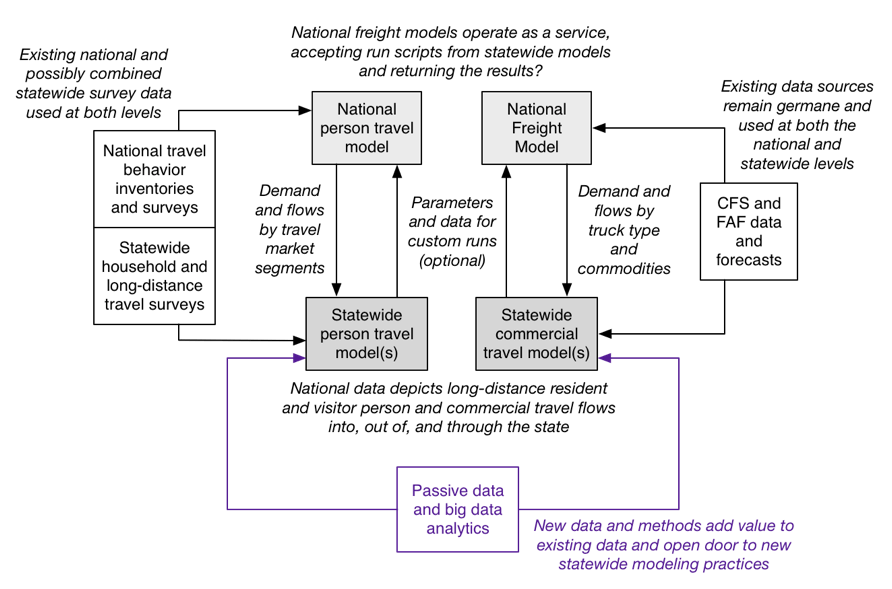
\includegraphics[width=6.5in]{graphics/41-integrated-modeling-opportunities}  
\caption{A vision of integrated statewide-national modeling opportunities}
\label{fig:integrated-opportunities}
\end{figure}

Such a system is neither far-fetched nor fanciful. Such capabilities have long been sought by statewide modelers, and it is thought that such models could place the state within its national context. Perhaps more importantly, it would substantially reduce the costs borne by the states for each to mimic such capabilities.

\section{Strategic visioning models}\label{sec:strategic-visioning-models}

While a standard practice of statewide modeling has yet to emerge, it is safe to assert that most are built using the traditional trip-based modeling paradigm, with flows assigned to a statewide or regional transportation network. In a few cases, states and researchers have experimented with lightweight scenario evaluation models over the past decade, and have found them to be useful adjuncts to the models described in this report. Such models are often described as sketch planning, scenario evaluation, or strategic planning models.

One visioning model designed for statewide modeling was developed by the Oregon DOT. They developed their GreenSTEP model in-house to quickly assess a wide range of potential greenhouse gas emission reduction strategies. The model starts by generating synthetic households across the state. Typical travel patterns mined from the NHTS are applied to households, based upon their characteristics. Aggregate measures of travel are obtained, such as vehicle miles and hours of travel per household. Finally, greenhouse gas emission calculations are carried out to characterize Oregon's footprint.

Mobile emissions of greenhouse gasses are not as influenced by vehicle operating cycle as other emissions, so a simpler congestion model is used to allocate VMT to speed bins. This obviates the need for a detailed network model to obtain accurate estimates. Moreover, the results are compared to statewide reduction targets, reducing the need for the higher levels of spatial, temporal, and behavioral resolution found in current statewide models. Because of the focus on greenhouse gas emissions, the model pays much more attention to vehicle and fuel characteristics than do traditional travel demand models.

A key advantage to using GreenSTEP is its ability to very rapidly assess many alternate futures. Changes in demographics can be easily handled, and the analyst can also change the distributions and rates obtained from the NHTS to evaluate the extent to which current choices would have to change to meet Oregon's greenhouse gas reduction targets. Although applied at the state level, households could be segregated by planning region or metropolitan area to examine outcomes by sub-state areas.

Several variants of GreenSTEP have been developed, including ODOT's Regional Strategic Planning Model (RSPM), FHWA's Energy and Emissions Reduction Policy Analysis Tool (EER\-PAT), and AASHTO's Rapid Policy Analysis Tool (RPAT). An effort is now underway to refactor these models in the new VisionEval model system and software framework to enable model components to be more easily shared between models and to enable the model system to be more easily expanded with new components.

What has not yet happened is tighter integration with mainstream models. Such could be accomplished through the linkages illustrated in Figure \ref{fig:visioneval-swim}. Note that this concept and illustration are ideas of the author, not part of the Oregon Modeling Improvement Program or official plan. Selected scenarios from a VisionEval model could be pushed to the statewide model for closer study, while the more detailed travel characteristics from the statewide model, estimated from their statewide household travel survey, could be used in place of the more generic NHTS estimates of travel behavior. The benefits of using both types of models together seem likely to exceed the value of either alone, and is proposed as an opportunity for expanding the tools available to statewide modelers.

\begin{figure}
\centering
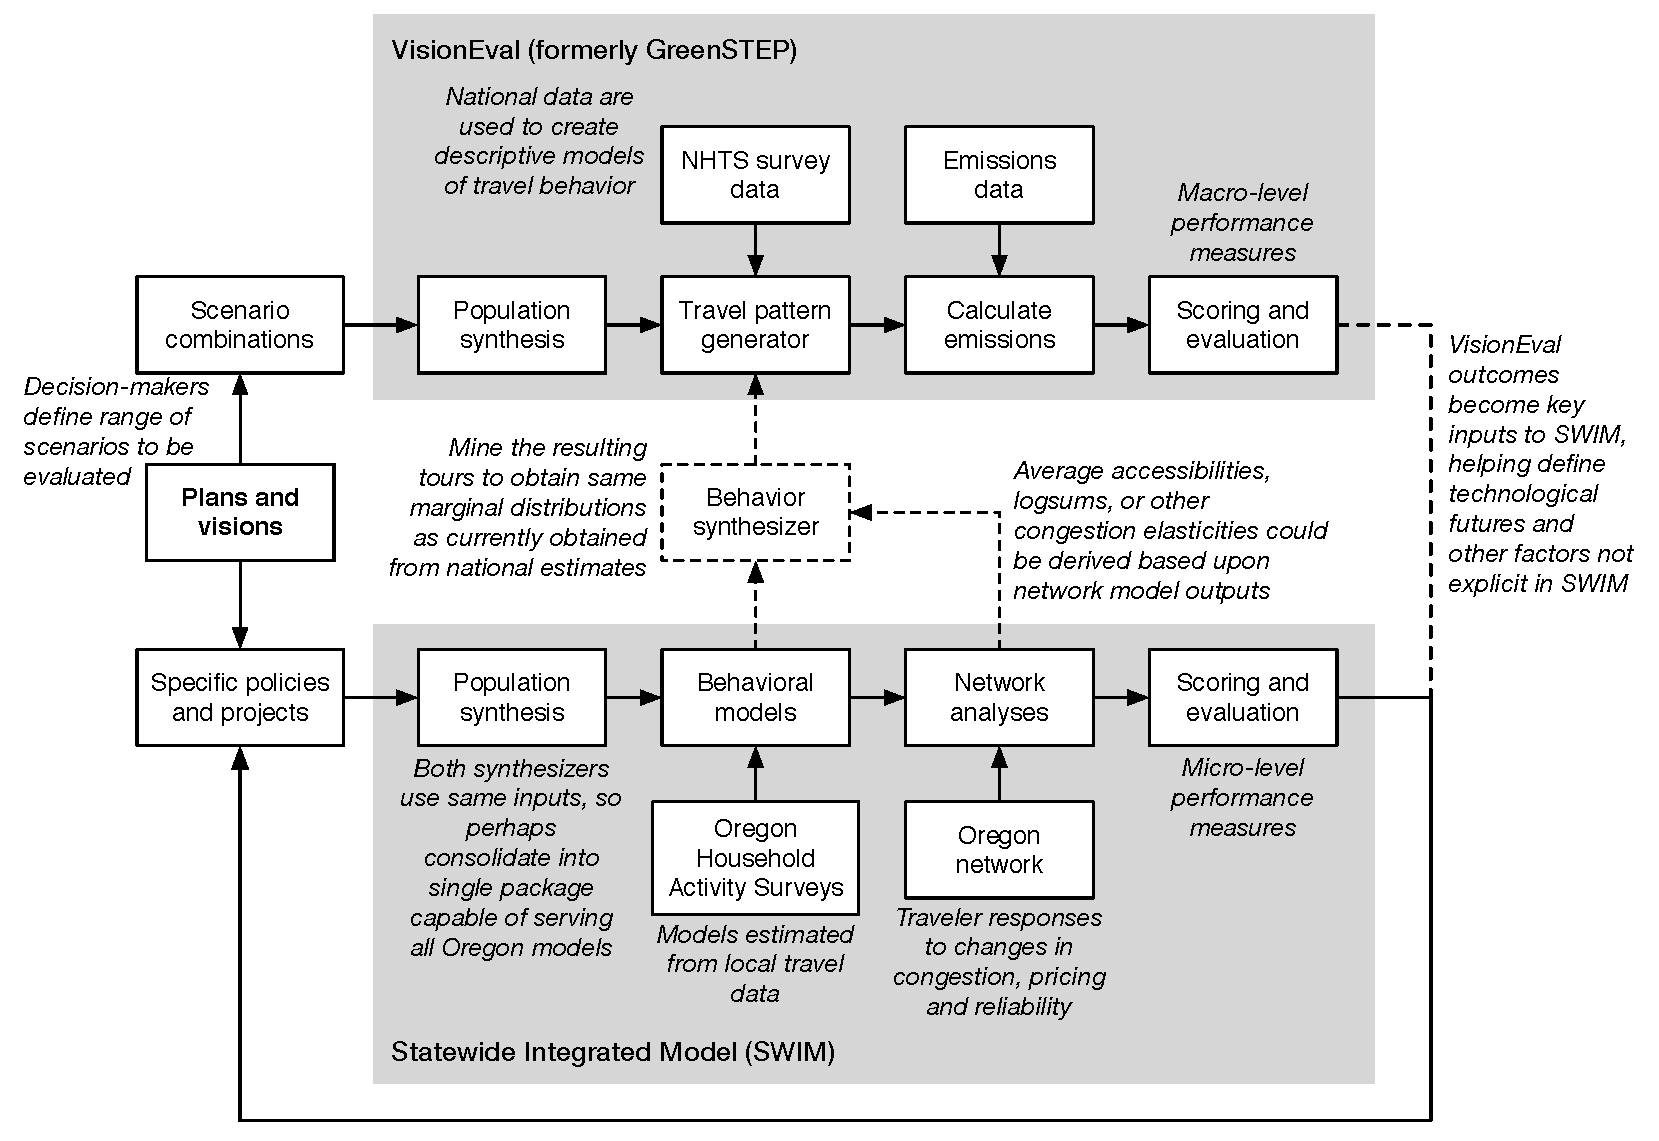
\includegraphics[width=6.5in]{graphics/42-visioneval-swim-integration}
\caption{Hypothetical framework for unifying Oregon visioning and statewide models}
\label{fig:visioneval-swim}
\end{figure}

\section{Navigable networks}

The development of most statewide model networks is an expensive and ad hoc process. It is reported to be among the most onerous parts of statewide modeling, as noted in \S\ref{sec:network-representations}. None of these take advantage of the routable networks used for personal and vehicular navigation systems. While none of the various technology companies that provide such systems, such as Google, Waze, and Apple are known to share their network information, a great deal of interest was expressed by model developers to use them. There are formidable obstacles associated with doing so, to include the likely licensing terms and cost involved. The former may restrict usage of the data to periods when licensing or subscription is in effect, and the annual costs might be much higher than the one-time investment made in most statewide networks. Moreover, the networks themselves lack many of the attributes used in traditional traffic assignment methods. Some might easily be imputed, but others, such as functional classification, might require conflation of navigable networks and traditional network line layers.

If navigable networks became available, they would invite us to rethink how we carry out network analyses in all types of transport models. Widely-used macroscopic assignment models yield closed-form solutions even in hyper-congested states, but are sensitive to assumptions about the relationship between congestion and travel time (expressed as link capacity functions) and link attributes that are often coded by functional classification of the link. Navigation systems find time-dependent optimal routes through congested networks without knowing most of that information. Moreover, such systems have a history of observed travel times that can be flexibly defined by the analyst (e.g., hourly, variations by week). Such information cannot be known for facilities or services that do not exist or might be substantially different in the future. However, in systems where new infrastructure is being built less frequently such data-driven routing heuristics might become a viable alternative to current traffic assignment models.

Dynamic network models are also increasing in popularity, and several researchers have investigated their suitability for statewide modeling. \cite{erdogan14} investigated the use of dynamic traffic assignment (DTA) in Maryland, using a prototype version in TRANSIMS. It was thought that DTA would provide a better estimate of travel times experienced by travelers in the highly-congested Baltimore-Washington corridor. MATSim has been used for network analyses in several national models in Europe, most successfully in Germany. Several of our survey respondents ranked DTA as high on their list of desired model enhancements. Planning-level DTA procedures, which use essentially the same node-abstract representation of roadways as do macroscopic models, seem ideally suited to the task. This obviates the need to represent traffic signals across the state explicitly, which would be a Herculean task for most states to code or maintain timing plans for.

Activity-based models, now used in many major metropolitan areas, are often based on microsimulated households whose full attributes are carried through the simulation. No information is lost along the way, enabling flexible and sophisticated data mining of model results and detailed analyses of market segments. The same approach is gaining traction within statewide modeling. In essence, activity-based models synthesize a travel diary for each simulated person and household. Individual vehicles in dynamic network models can be associated with these diaries, enabling the modeler to better understand the population using a specific facility, an hour of the day, or other grouping variables.

\section{Multi-state models}

Many of the models we reviewed incorporated parts of adjacent states, some of which had almost as much detail as the statewide model in that state. Urban areas beyond the state border, especially when they are agglomerations, heavily influence both person and freight traffic patterns. The ability to bring the effect of important nearby markets into the model was one of the driving motivations for building the Chesapeake megaregional model. The benefits obtained from doing so were clear. There has been surprisingly little interest in consolidating resources by building multi-state or megaregional models, despite the apparent benefits. Several reasons were cited for this:

\begin{itemize}
\item Lack of control over model design, development priorities, or delivery deadlines
\item Increased effort required to run the model, owing to increase coordination with and data supplied by other states involved
\item Unique analytical requirements that other states do not have
\item Desire to retain capability to quickly adapt or change the model if required to meet new analytical requirements
\end{itemize}

These requirements appear to outweigh the potential for cost and data-sharing, and ability to satisfy common goals for model functionality and elimination of boundary effects at state borders. Moreover, computational and institutional issues will need to be overcome before multi-state models emerge in practice.

\chapter{Building a statewide model for state needs}\label{sec:building-models}

There is broad consensus on best practices for trip-based travel models in urban areas, and an abundance of literature to inform the development. Activity-based person travel models likewise tend to have similar components, with choices arranged in comparable order, despite their continuing evolution. Developers and users of such models can point to the best features of each, and a considerable of research is underway to improve them. It is more difficult to portray a typical statewide travel model. They address a wider range of requirements, cover much larger areas, and focus on markets that are not as well understood as those in urban areas.

This chapter attempts to overcome that by describing how such models are built, and the resources required to do so. It begins with a discussion of the foundations necessary to undertake statewide modeling, to include the geographic extent of such models, and how the economy, society, and transportation networks are represented. Trip and activity-based person and freight travel models are described in the following sections. They are followed by an examination of issues relating to integrating urban and statewide models, model validation, and the computational burdens associated with statewide modeling.

It is important to note that this chapter does not attempt to describe best practices in statewide modeling. What is best for any given agency is contextual, defined by their intended uses of the model. The best model is arguably one that addresses their needs promptly, with the least amount of investment, and which their staff can creatively and competently apply. Those dimensions are not addressed in this chapter. Rather, an attempt is made to define the state of the art and likely costs and benefit of pursuing it.

The costs described are based upon a review of the data collected for this report, costs described in the literature and model documentation, and experience of the authors. The costs shown for data are only for their acquisition. The cost of transforming them into models is stated in terms of typical additional cost for consultants to do so. Ideally, this work would be done by agency staff, to instill the skills and institutional knowledge required to maximize the investment in data and models. The cost savings associated with doing so are not addressed, for they likely vary widely.

The discussion of options presented in this chapter is limited to operational models, or those close to becoming so. There are many promising lines of ongoing research that might change how we build and use statewide models, as well as prototypes built by researchers and practitioners alike. However, these are typically not mature enough or proven in practice to include here. Moreover, it is difficult to guess at what data requirements they might have or their full cost of implementation.

\section{The modeling environment}

We can consider the modeling environment apart from the models applied within it. The former includes how the demographic and land use markets in the modeled area are represented, as well as the multimodal transportation network and service providers. The state and regional economy are increasingly being represented in statewide models are well. Most often decisions about the desired levels of spatial, temporal, and behavioral resolution are made on this basis. That is, the agency's needs frame the required level of detail in the model, not the other way around. However, those parameters differ by model component. The economy, land use, and travel choices all evolve at different rates, and are best represented at different geographic and time scales. This is especially true for long-distance models, where it is usually sufficient to know the state or megaregion of distal trip ends.

Early statewide models tackled the issue of conflicting resolutions by modeling the entire system at the highest level of resolution required for any of its components. Such an approach makes sense when only modeling travel choices. However, attempting to model the regional economy at the traffic analysis zone quickly proves intractable, for the rich time series of macroeconomic data extends from the national level down to counties, but not below it. It is possible to divide the data into successively smaller units, but a more flexible approach is to develop modeling systems that operate at multiple levels. There is a long tradition of doing so for freight models that can be extended into statewide models. \cite{xu03} describes a multi-level national model, in which financial, supply chain, and transport markets are represented at different levels of resolution, as shown in Figure \ref{fig:multi-scale-modeling}. Microsimulation approaches are more amenable to operating at several levels than aggregate models, making these easier to integrate into activity-based models.

\begin{figure}  % 43
\centering
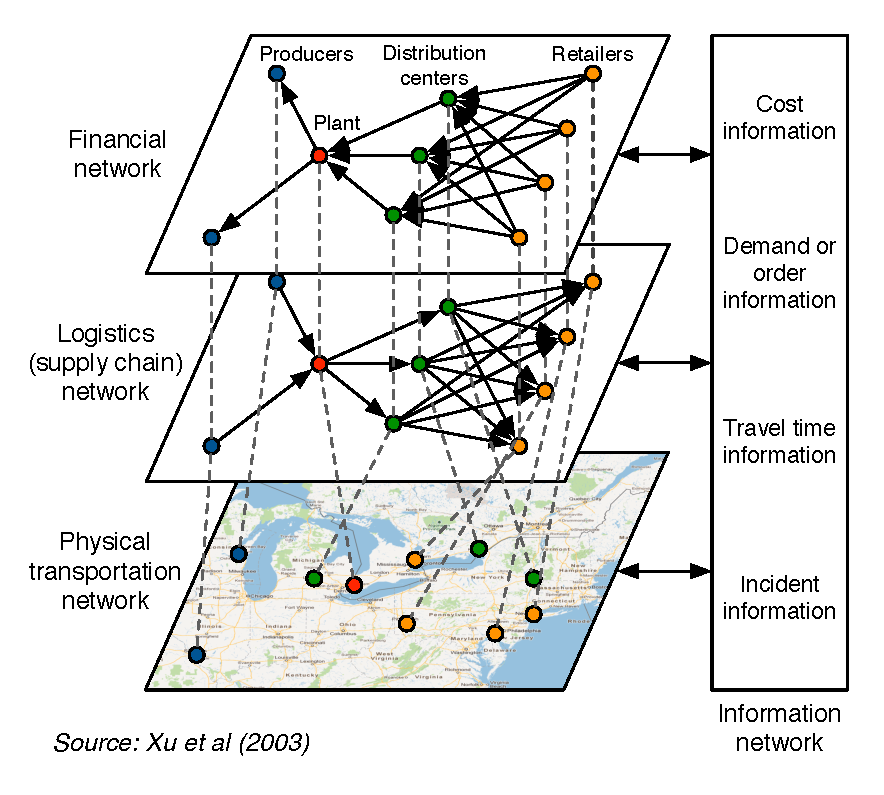
\includegraphics[scale=0.6]{graphics/43-multi-scale-modeling}
\caption{Multi-scale modeling framework}
\label{fig:multi-scale-modeling}
\end{figure}

A model incorporating multiple levels of geography can also use networks scaled to each, although no operational model is known to do so. Rather, most analysts aggregate travel time and distance skims from the statewide model to levels represented at coarser levels of geography, providing them with measures of spatial separation instead of multiple networks. Agents representing households and firms can easily incorporate data from different levels, while reconciling flows between networks of differing resolution remains a very difficult proposition.

\subsection{External markets}

Many decision-makers are interested in knowing from where people and goods move into and out of the state. This is especially true in so-called ``bridge states,'' who feel the impact of large numbers of through trips that do not contribute to its economy. This is also true for freight shipments, which are increasingly part of global supply chains. Representing these external markets, and the flows coming to and from them, has historically been a challenge for statewide modelers. The amount of work required to explicitly include them, as well as the paucity of data, have limited the options for modelers.

Building an external zone system that covers the rest of North America, and populating it with Census and Commerce data about aggregate activity levels, is straight-forward. Obtaining forecasts for those attributes, on the other hand, has historically been challenging and expensive. However, even more difficult was obtaining robust data on the person and freight flows between them. This changed quickly for freight with the introduction of the FAF (\S\ref{sec:traditional-freight-data}), which has improved continually since then. Using the 146 FAF regions covering North America to represent the rest of the continent makes summarization of these data simple.

Comparable data are not available for long-distance person travel, except for the small amount of NHTS long-distance data coded to the Census region level. This obviates the need to consider their geographic representation in addition to, or in lieu of, the FAF regions. If the national person and freight models described in \S\ref{sec:national-model-integration} were to become operational their data would be available at much finer levels of geography. Including the FAF regions as placeholders for their eventual use will quickly add a national context to existing models.

\subsection{Macroeconomic data and models}

Most states use economic forecasts prepared by third parties, including other state agencies and commercial products. The types of data provided range from employment estimates to gross state product by industry that vary by level of geographic and industry detail, and how far into the future estimates are provided for. Many only include the state being modeled, although several states have calculated the growth rates implicit in the FAF to learn where growth in external markets is likely to occur.

Incorporating economic forecasts into existing statewide models is straight-forward, although they are typically provided at the statewide or metropolitan region level. Using these data to drive future estimates of population and employment, either at the zonal level or in synthetic populations, is relatively straight-forward.

A few states have attempted to include an economic model within their statewide modeling system. This is normally done within the context of an integrated economic-land use-transport modeling system, such as those in Ohio and Oregon. An agency might consider building such a model to create better and more internally consistent demographic forecasts. They might also wish to evaluate how changes in travel costs and accessibility influence economic growth, or the consequences of loss or degradation of portions of the network. However, the costs associated with building such a model, and the multi-year development cycles, often make this a prohibitively expensive undertaking unless dictated by agency or legislative reporting requirements.

\subsection{Multimodal networks}

Building and maintaining networks remain a heavy burden at all levels of travel demand modeling, as discussed in \S\ref{sec:network-representations}. Advances in this realm have been small compared to other aspects of modeling. Most statewide models appeared to only include major arterials and higher functional class roadways within the state, and Interstate and numbered U.S. highways outside of it. The National Highway Planning Network or Oak Ridge Network (used for coding the CFS and assigning FAF flows) are typically adapted for this purpose. Fixed guideway and intercity rail transit lines are usually explicit, although local bus service is not. \cite{circella14} describe a straightforward method of synthesizing such coverage in statewide models that greatly reduces the burden associated with representing local transit service, and seems appropriate for most statewide models.

Additional network detail is often desired, to support project-level and small area analyses with statewide models. Indeed, some states do include all roadways, down to the collector and local road level, in their models. None have documented benefits other than the ability to support detailed analyses, or the additional cost involved. Thus, we can only rely upon anecdotal evidence that suggests that doing so greatly increases the amount of work involved. Whether it is worth the investment is a question that only the agency can answer.

\section{The modeling approaches}

Most statewide models are trip-based formulations, very similar in structure to comparable urban models. They often have simplified or no mode choice models, especially in places where intercity transit has a very small market share. Those that have trip-based person models are also likely to have trip-based freight models as well. Many of these models are created with transferred or synthetic data, as revealed in Table \ref{tab:data-combinations} (page \pageref{tab:data-combinations}). Only three states --- California, Ohio, and Oregon --- have implemented an activity-based person modeling approach, all of which also use tour-based truck models.

\subsection{Trip-based person modeling approaches}

The trip-based modeling paradigm is well established, with well-known requirements for their development and deployment. Several states have built models that meet their needs with no more than such knowledge, transferable parameters from the NCHRP reports listed in \S\ref{sec:traditional-person}, and summaries derived from the ACS PUMS data and NHTS microdata. They almost always lack a mode choice modeling component, but are otherwise a competent implementation of best practices in trip-based models. Thus, it is demonstrably easy to build a first-generation model once the initial, and often costly, investment has been made in developing the modeling backplane.

There are several paths past this initial implementation when remaining within a trip-based modeling paradigm. An exhaustive list is beyond the scope of this discussion, but some of the most commonly pursued paths include:

\begin{itemize}
\item
Some states have conducted statewide travel surveys, fused urban travel surveys within their state (and sometimes adjacent ones), or relied upon urban surveys for those with one dominant metropolitan area, to derive trip characteristics used in the model (e.g., trip production and attractions, trip length frequency and time-of-day distributions). Michigan and Oregon have fielded surveys designed to capture adequate samples in different regions of the state. The existing model can be updated using these data, or extended with new features or greater detail.
\item
Other states need to develop mode choice and network assignment capabilities that facilitate pricing analyses. The auto nest of urban and intercity mode choice models can be extended to include pricing, which requires asserting and calibrating the coefficients associated with the new sub-nest(s), based on experience elsewhere, or conducting or adapting additional RP or SP surveys. An RP/SP survey of the size and scope recently conducted for the California HSR modeling work, described in \S\ref{sec:california-hsr-model}, is necessary for estimating a model specific for the modeled area. The cost of that survey was approximately \$350,000. Thus, depending upon the data available and approach chosen this enhancement likely represents a significant investment.
\item
Replacing a traditional trip distribution model with a logit-based destination choice model often leads to improvements in model validation and explanatory power. Such models are usually estimated using existing travel survey data, which often requires adding occupation to the list of variables generated for synthetic populations or zonal estimates. However, the recent availability of OD matrices based on cellular tracking, with their ability to partition flows by residents versus visitors and trip purpose, is a huge advance that will revolutionize travel modeling. Their cost depends upon the geographic scale and duration of data provided. The expected cost of these data, ranging from \$250,000 to \$2M, should be factored into the cost of all statewide models in the future.
\item
Visitor models can be built in several ways. Two broad approaches for doing so have emerged. One uses the same cellular tracking data described above to create visitor flow matrices, to which growth factors can be applied when forecasting. The alternative is to build a synthetic model, based upon the slim survey data available and counts of travelers by mode. \cite{moeckel11} describe how such a model was implemented in several states.
\end{itemize}

The options for enhancing trip-based models are summarized in Table \ref{tab:tripbased-enhancements}. The effort required to improve trip-based models are modest compared to those for developing more advanced models. Those states that can meet their needs with such models will reap significant advantages from such cost-effective incremental improvements. Possibly even larger efficiencies could be gained by pooling funds to conduct travel surveys across several adjacent states, although no such effort has been reported.

\begin{table}  % 5
\centering
\caption{Common enhancements to trip-based models}
\label{tab:tripbased-enhancements}
\begin{tabular}{L{1.8in}L{2in}L{2.2in}}
\hline
Model enhancement & Additional data required & Estimated cost \\
\hline
Implement base model based upon synthetic or borrowed parameters & None & \$50,000 to \$250,000, depending upon desired features, level of detail, and other design issues \\
\gray Update or improve existing model & Statewide household travel survey & \$1.5-8.5M, depending upon survey design and sample size \\
Add mode choice models capable of addressing traveler responses to pricing & Statewide household travel survey of adaptation of existing urban surveys, possibly augmented with RP/SP survey & Costs shown above for travel survey, plus \$150,000 to \$300,000 for model development, and \$500,000 for RP/SP survey \\
\gray Implement destination choice model & LEHD data and analyses & \$50,000 to \$100,000 \\
Implement destination choice and visitor models based upon cellular tracking data & Third-party cellular tracking data (e.g., AirSage, StreetLight) & \$250,000 to \$2M, depending upon type and resolution of data specified, subscription terms, etc. \\
\gray Synthetic visitor model, based upon simulation of NHTS or comparable data & None & \$100,000 \\
\hline
\end{tabular}
\end{table}

\subsection{Activity-based person travel models}

The decisions in all three states that have pursued advanced person travel models were based upon analytical issues thought to be difficult to address with trip-based models. Moreover, each had a highly motivated and accomplished champion within the agency committed to the significant advances required to achieve such goals. Thus, there are too few statewide activity-based models from which to generalize development and data requirements and trends from, made more difficult by the fact that two of the three implement them within a larger (and even rarer) integrated economic-land use-transport modeling framework. However, lessons learned from the implementation of comparable models in urban areas, as well as their experiences, can be instructive.

Model developers typically assert that the same data required for best practices person trip-based models will suffice for the development of activity-based models. Thus, it is likely that the types of data required and resources required to develop them depend more upon the desired levels of spatial, temporal, and behavioral resolution desired, and the anticipated level of market segmentation, than the choice of modeling paradigm. The choice models included in such models are considerably more sophisticated than those found in aggregate models, even though most could also be implemented within a trip-based modeling framework.

One of the more common additional data requirements is the classification of households and businesses by occupational categories, in addition to industry classification. This permits more precise matching of households with appropriate jobs in workplace location models. Such relationships can be gleaned from the Longitudinal Employment and Household Dynamics (LEHD) database, available from the Census Bureau. However, processing of these data requires considerable familiarity with their contents and limitations.

There are about two dozen operational activity-based models across North America, with a half-dozen more known to be under active development. The San Diego model was transplanted to the Miami region, at the cost of about \$1 million. Thus, the cost of building an activity-based model at the statewide level, which would likely incorporate the enhancements described in the previous section for trip-based models, likely ranges from one to several million dollars. It further depends upon the desired functionality, amount of new model estimation required, new features, and data collection required to accomplish it.

There are many potential benefits that can be gained from such an approach, but in practice the most compelling appear to be their superiority over traditional models for pricing and equity analyses \citep{donnelly10}. The microsimulation framework enables full information about the traveler and trip to be retained throughout the model, as well as variation of rules and parameters across different geographic and market segments. The resulting model output is a simulated travel diary for the entire population, which can flexibly be mined and summarized based upon the analyses at hand. Whether such benefits are compelling enough to justify their investment depends upon the goals of and resources available to each state.

An alternative to implementing a full activity-based model all at once is to incrementally move towards it. A trip-based model can be updated in steps, spreading the cost over several years, obtaining some benefits earlier, and enabling staff to gain familiarity and confidence with each part before making further changes. This enables the benefit of each improvement to be measured and understood, and the ability to drop those new features or formulations that fail to deliver them. Such a gradual transition typically starts with the implementation of synthetic populations and replacement of the trip generation module with a daily activity patterns model. Subsequent modules are then replaced over time.

An illustrated plan for the transition of Maryland's statewide model, prepared by the authors, is shown in Figure \ref{fig:maryland-evolution}. The cost associated with gradual transition are most likely no different in total, or slightly higher, than the development of a full activity-based model. They can be spread over time, however, and possibly redirected as agency requirements change.

\begin{figure}[!t]
\centering
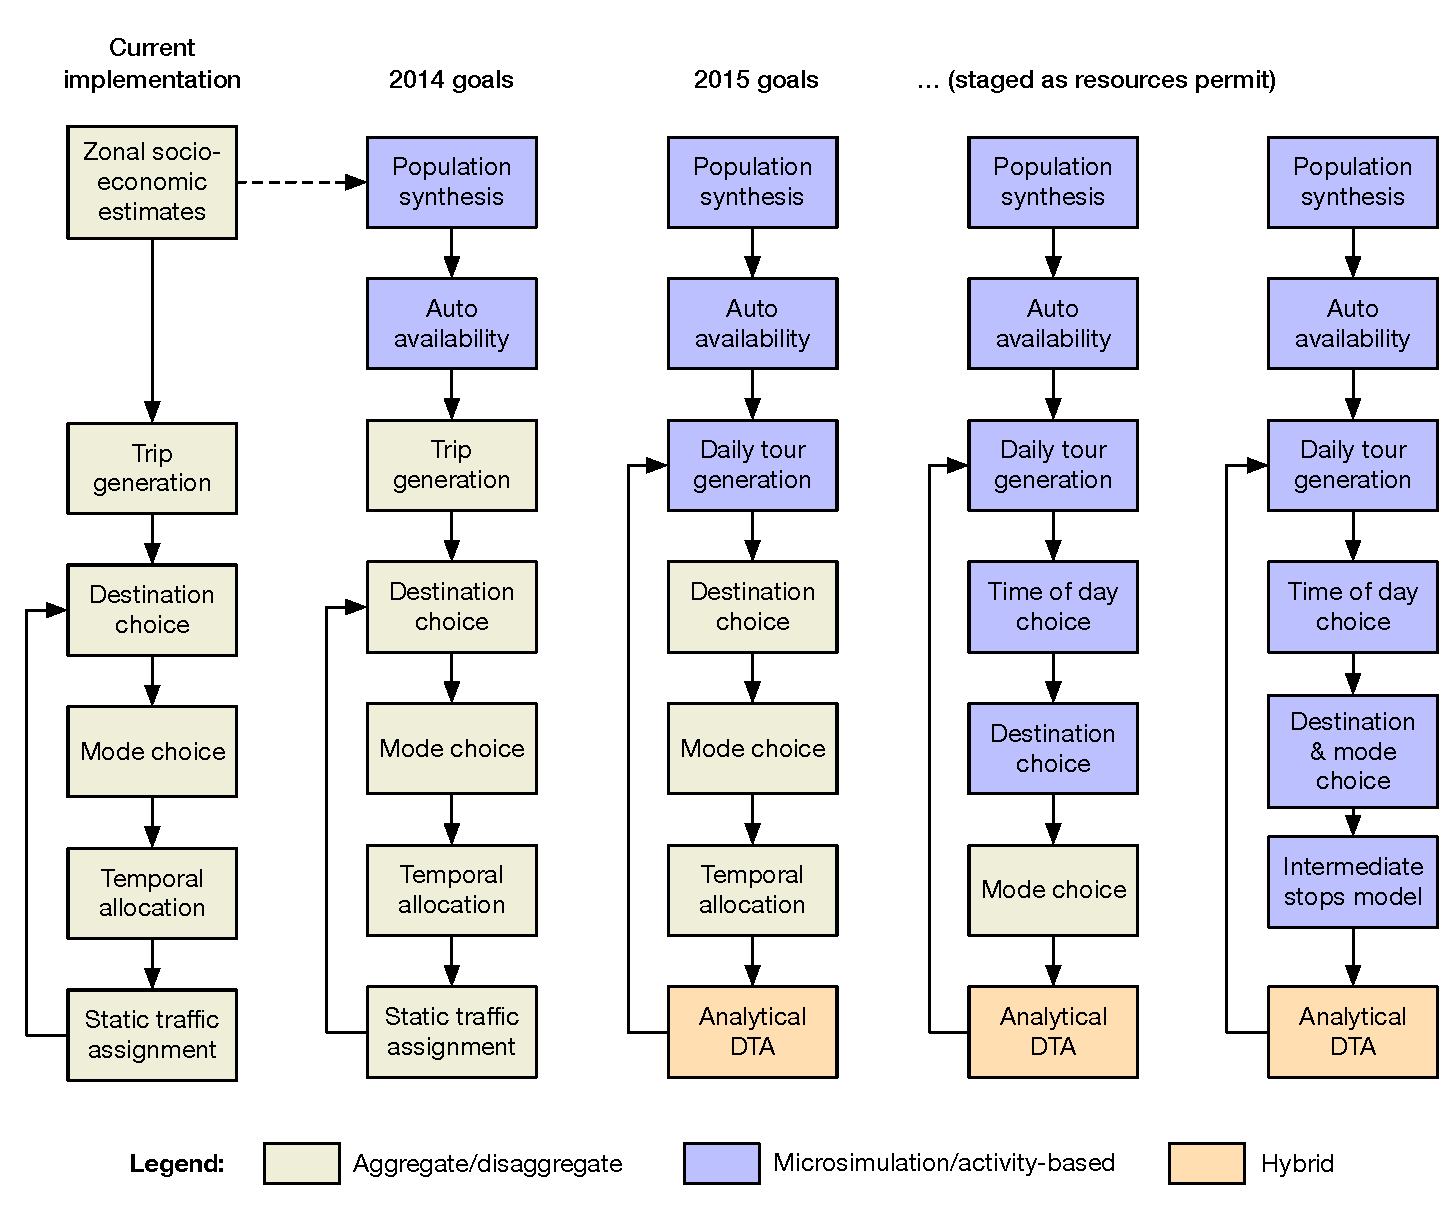
\includegraphics[width=6.5in]{graphics/44-maryland-model-evolution}
\caption{Transition from trip-based to activity-based framework in Maryland}
\label{fig:maryland-evolution}
\end{figure}

\subsection{Trip-based commercial vehicle models}

There is a considerable amount of literature devoted to freight modeling at several levels of resolution, ranging from urban truck models to inter-regional commodity flow models, to international trade forecasts. Most can be classified as either truck or commodity flow models, and local versus long-distance. The best practices in trip-based freight modeling are assembled in the FHWA \textit{Quick Response Freight Manual II} (QRFM)\citep{beagan07}, which use the same data required for person travel models. This approach can be coupled with the use of FAF to quickly implement trip-based statewide freight models. The techniques described can be quickly implemented, albeit only at coarse levels of FAF geography without additional processing of the data. How well such models work within statewide models has not been reported in the literature, although their shortcomings have been widely acknowledged. The trip generation and distribution parameter estimates from the manual can be updated with values from other areas, or iteratively adjusted to better match observed truck flows. Both can be undertaken at low cost.

Most states have few highly reliable vehicle classification counts, and typically none within urban areas other than on major highways. These are often supplemented with manual counts, counts from urban areas, and data from HPMS, most of which use adjustment factors derived from those few automatic traffic classifiers to impute the percentage of truck flows by area type and functional class. The experience of the authors is that few investments have as large a payoff as increasing the number of vehicle classification counts within the state. Most of these must be done by contractors, as resources to expand the number of automatic traffic recorders are not available. Data on the cost conducting such counts were not collected in this research, but the experience of the authors suggests the costs runs between \$150,000 to \$250,000 to expand the number of vehicle classification counts across a state to a level that permits robust model validation and insight into unique flow patterns.

Moving beyond the QRFM or comparable models and expanded count data requires a considerable investment in data. Establishment surveys that include truck travel diaries are often suggested to gain data that captures unique local patterns, obtain finer market segmentation, a wider range of explanatory variables, or capture of non-freight commercial vehicle travel. \cite{hunt07} used such data, collected at the cost of about \$3.5 million, to build a commercial vehicle model for Calgary. They have transferred their model to several other places, including the first-generation California statewide model. The cost seems surprisingly high, until one considers how different combinations of firm classifications, size ranges, and truck categories expand the number of observations required. The number of levels within each dimension can be reduced, of course, but only with corresponding increases in variances associated with parameters derived from the data.

Many argue that establishment surveys alone cannot provide a holistic view of all truck flows within a city or region, much less flows by all modes of transport. \cite{roorda11} proposes the fusion of shipper-based surveys with third-party truck tracking data to better understand truck patterns. \cite{zmud14} suggest investments in a combination of a revived Vehicle Inventory and Use Survey (VIUS), third-party truck tracking data, and agent-based modeling to achieve the same ends. California's investment in a replacement for the VIUS, described in \S\ref{sec:ca-statewide-models}, represents an essential first step in achieving those goals.

The cost of such data programs varies, and there is not enough experience with them to generalize the cost and effort involved in conducting them. However, it can confidently be asserted that they are multi-million dollar efforts whose design, testing, execution, and processing will likely last two to three years. They can be designed as continuous collection efforts rather than single large, costly, and disruptive activities. Moreover, the potential benefits of multi-state collaboration on such efforts seem enormous, but have not been attempted to date.

\subsection{Advanced commercial travel models}

The benefits of representing the tour structure of urban truck trips, and the associated improvements in functionality and outcomes, are well documented. There appears to be as much progress in implementing such models at the statewide level as there is within urban areas, in fact. Oregon developed a microsimulation-based short-distance truck tour model in 2003 that has been subsequently overhauled and adapted in Idaho and Ontario. A similar adaptation of the Calgary model was implemented in the Ohio statewide model a few years later \citep{gliebe07}. The Calgary model was also implemented in the California statewide model, as discussed in \S\ref{sec:ca-statewide-models}. The Calgary adaptations took advantage of extensive establishment survey data collected earlier in Alberta, and used in its original development. The adaptations were calibrated to match locally observed patterns.

The cost of implementing these four models ranged from \$75,000 to \$150,000, exclusive of the cost of obtaining and preparing the establishment survey. However, the cost is a bit misleading, for the integrated economic-land use-transport modeling platform they worked within provided additional data required to build and use them. Make and use coefficients derived from economic input-output data are used to associate commodities with industries, as well as estimates of production and consumption by firms with each sector. The Oregon model was implemented without the latter until recently, making it an open question of how much data are required to implement such models, versus desirable. If implemented outside of an integrated model it is likely that the data requirements would include the elements shown in Table \ref{tab:freight-data}.

\begin{table}[!t]   % 6
\centering
\caption{Typical data requirements for advanced freight models}
\label{tab:freight-data}
\begin{tabular}{L{1.9in}L{1.8in}L{2.3in}}
\hline
Data element & Scale & Estimated cost \\
\hline
Database of firms and key attributes (e.g., size, NAICS code, location) & Firms & \$5,000-\$30,000, depending upon vendor chosen and number of attributes desired \\
\gray Establishment travel survey & Firms segmented by area, industry, size, type of truck(s) operated or contracted & \$3.5M, but depends upon survey design, sampling frame and rate, and recruiting strategies \\
Forecast of gross state product, employment, and percentage of employees by occupation & State or sub-state region & Highly variable, depending on source, length and granularity of forecast periods, industry detail, etc. \\
\gray Make and use coefficients derived from input-output accounts & State or national & Typically included in economic forecast, but can be borrowed from other areas or derived from national benchmark IO accounts \\
Commercial vehicle survey (optional) & Trucks by operator & \$250,000 to \$2.5M, depending upon survey design, coverage, sampling rate, and other factors \\
\gray Vehicle tracking data (detailed GPS traces of truck movements over long periods) & Trucks by firm & Costs difficult to estimate because of only recent availability, cost in Florida and Ontario differ significantly \\
Carload Waybill Sample data (optional, used to better understand rail flows and calculate modal accessibilities) & Sampled waybills & Cost to obtain these data from Surface Transportation Board is minimal, although accompanied by non-disclosure requirements limiting their use \\
\hline
\end{tabular}
\end{table}

The costs shown reveal the substantial jump in cost and effort required to go from trip-based to advanced freight models. There is little ground in the middle, aside from substituting survey data collected elsewhere for locally collected information. Some states additionally represent rail flows, at least in aggregate, although analyses appear limited to the depiction of high-volume rail corridors and terminals. Thus, type and extent of data required will likely vary by type of model, modes of transport represented, resolution, and other factors. The data shown in Table \ref{tab:freight-data} should be used only as rough guidelines.

It is likely that more sophisticated freight models will eventually replace the current crop of models, both at the urban and statewide levels. \cite{chase13} outline the knowledge, data, models, and sharing required to improve the practice of freight modeling, although there are several competing proposals. A national freight model, if it were to come to fruition, would also dramatically change the freight modeling landscape, as well as substantially reducing the cost. Whether a given state can wait for those proposed initiatives to come to pass, or need to gain such capability earlier, is dictated by the issues and requirements they face.

\section{Urban-statewide model integration}\label{sec:urban-statewide-integration}

The approaches used for statewide modeling vary considerably, as noted in Chapter \ref{sec:survey-existing-practice}, especially with how they represent urban areas that have their own travel demand model. In some cases, statewide modelers attempt to use spatial, temporal, and behavioral resolutions more commonly found in urban areas, but stretched to cover the entire state. In other cases, a more abstract representation is used at the statewide level. Irrespective of the approach taken, it was expected that a great deal of effort would have gone into tightly integrating urban and statewide models. The use of common data would lend consistency to both models, even though each operated at different scales, and typically focused on different travel markets.

Instead, we found that such high-level coordination was rarely undertaken. Many states attempted to use aggregations of urban traffic analysis zones in areas where the two models overlapped, and many others reported a desire to replace external trip data and models at the urban level with long-distance travel data from the statewide model. However, many developers we interviewed expressed little need for or interest in tightly integrating urban and statewide models. It was felt that GIS techniques made conflation of demand data from heterogeneous zone systems practical when needed, yet freed developers of each model from having to coordinate the addition of new zones. The difficulties of maintaining a common network were cited even more frequently, suggesting that there was not as much overlap in the type and scale of analyses conducted with each modeling system as might be imagined. 

\section{Economic impact models}\label{sec:economic-impact-models}

Several states have adopted economic impact models to better inform project and program evaluations. Such platforms can be used to quantify the first and higher economic effects of proposed investments on the local and regional economy, multiplier effects, and potential revenue implications. Two examples of how statewide travel and economic impact models might interact are shown in Figure \ref{fig:economic-impact-models}. Indeed, some of the latter are as sophisticated as the former. The data requirements of these platforms will influence the design of the statewide model, as the value of seamless exchange of data is clear. There are no known instances of statewide models incorporating the results of these economic impact models, although the integrated models in Ohio and Oregon are designed to accept such feedback.

\begin{figure}[!t]   % 45
\centering
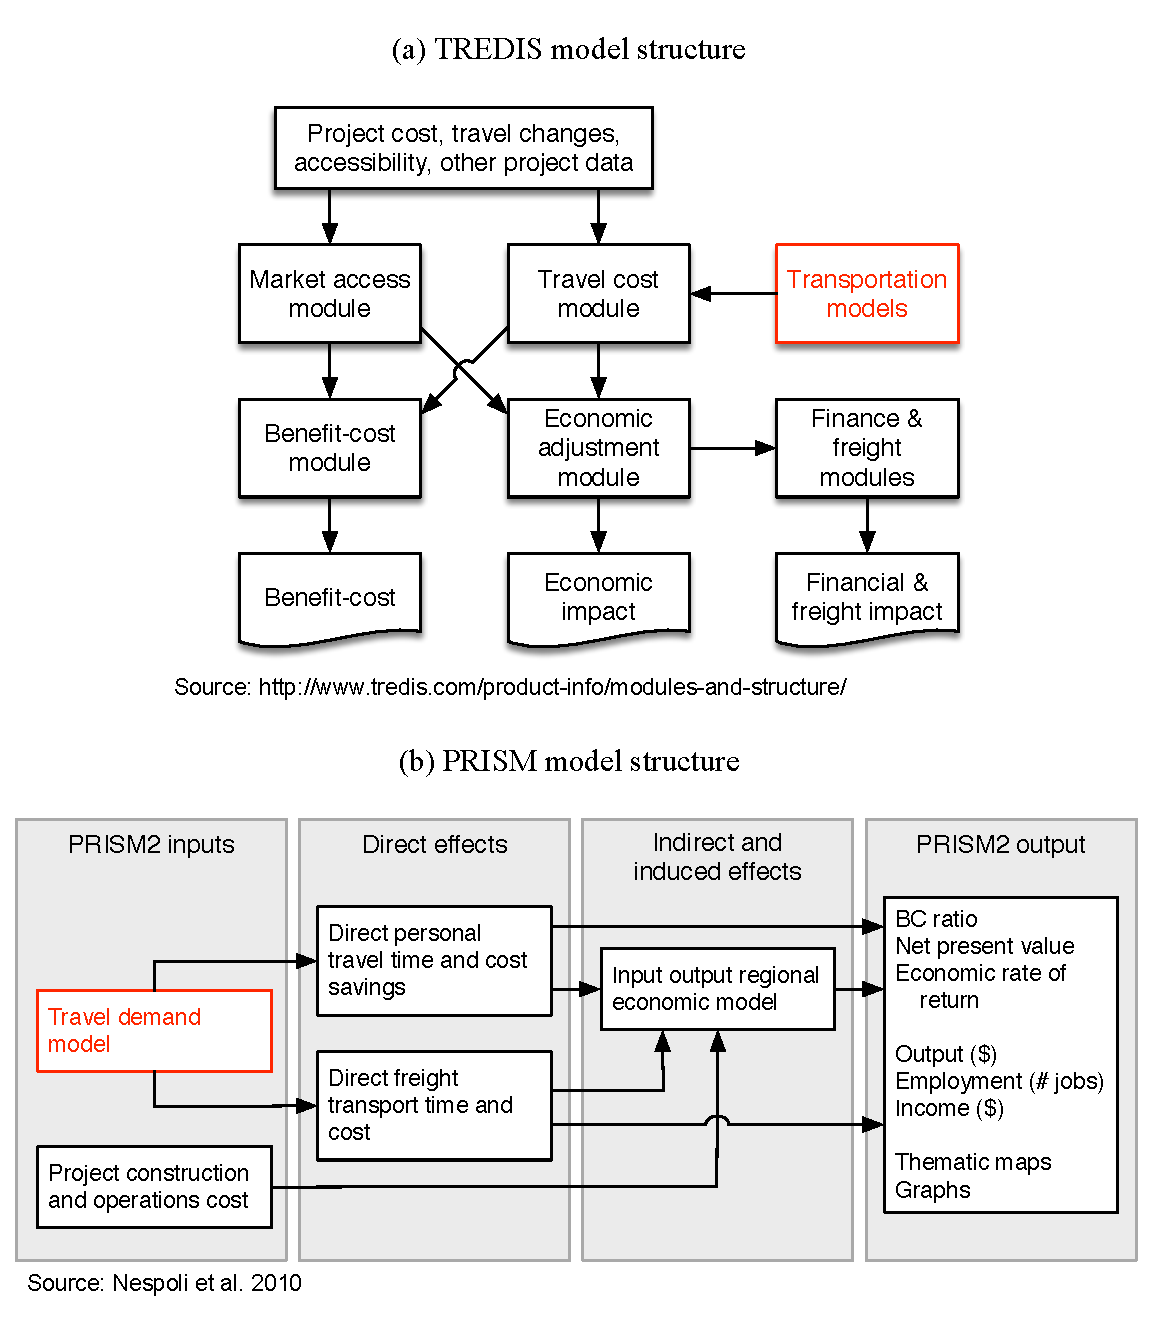
\includegraphics[scale=0.7]{graphics/45-economic-impact-models}
\caption{Examples of travel models within economic impact modeling frameworks}
\label{fig:economic-impact-models}
\end{figure}

The value of coupling statewide travel and economic impact models should not be dismissed. Oregon could use their statewide model to pose bridge deterioration as an economic issue affecting jobs, economic vitality, and market connectivity. It was not linked to an economic impact model, but because of its integrated economic-land use-transportation structure it could be used to demonstrate the impacts of bridge closures and restrictions. The Oregon legislature approved a \$4.8 billion bridge improvement program, based largely on the compelling evidence of economic impacts supplied by the statewide model. Couching an infrastructure problem as an economic issue was a wise move, for arguing the case based solely on the engineering issues was thought to have attracted far less support by legislators. It is a statewide modeling success story that deserves to be widely repeated, and a cogent reminder that a successful statewide modeling program should encompass more than just travel forecasting models.

\section{Model validation}

There is scant guidance on appropriate validation criteria for statewide models, or how they might be interpreted. Statewide modeling presents some unique challenges in this regard. The scant data available on long-distance travel and the unique characteristics of rural travelers dictates that they are consumed in model estimation and calibration, leaving few available for validation. This is even more true for commercial vehicles,  whose underlying business and travel patterns have much wider variances associated with them. The topic of freight model validation is rarely addressed in the literature, and definitive guidance on appropriate performance measures and testing procedures at either the urban or statewide level are lacking.

\cite{cambridge10} evaluated of validation practices and outcomes used in 11 of the 32 statewide models they reviewed, which remains a singular work in this area. They examined the structure and typical uses of these models, which revealed they covered wide ranges, precluding a single set of benchmark tests and standards. Differences in market segmentation frustrated attempts to isolate patterns in the data, and even otherwise similar models were found to have a wide range of reported parameter estimates. They cited several sources of data that could be used in validation, but the Highway Performance Monitoring System (HPMS) was the only one that is not commonly used in model development. We found no evidence in our review that validation practices have evolved since then.

The criteria used in different states were found to vary considerably, as shown in Figure \ref{fig:validation-practices}. Information from three additional models has been added by the authors, which does not change the earlier finding that most states relied solely upon measures of how well the modeled flows replicated observed flows. Statistical measures commonly used in urban models, such as root mean square error (RMSE) by functional class and count volume range and screenline comparisons, also dominated the evaluation of statewide models. Independent estimates of vehicle miles of travel by county from the HPMS are also widely used to test model performance. Comparisons of average auto occupancy were the only tests widely carried out beyond the assessment of traffic assignment outcomes.

\begin{figure}[!t]
\centering
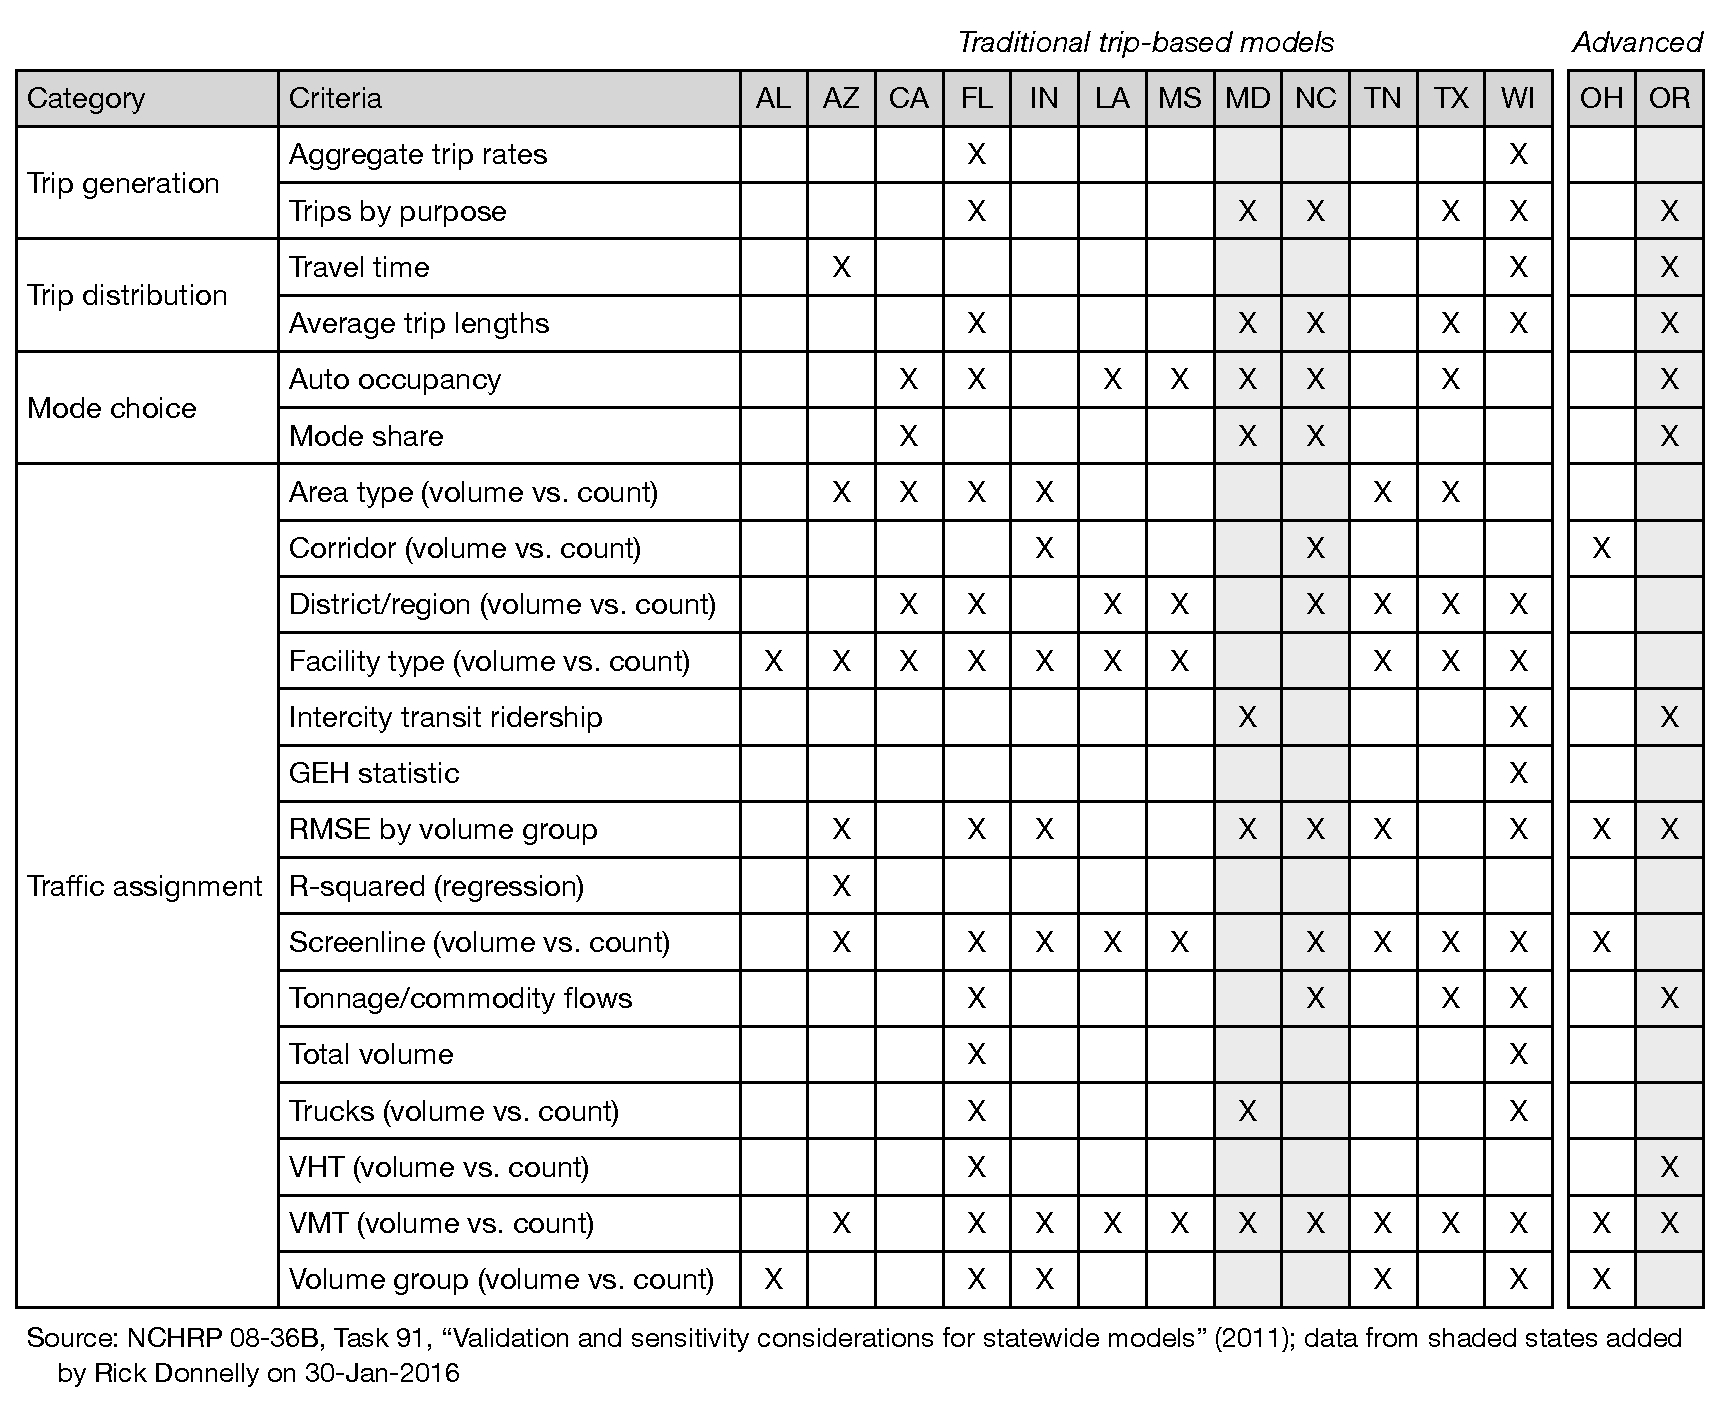
\includegraphics[width=6.5in]{graphics/46-validation-practices}
\caption{Validation practices employed in statewide modeling}
\label{fig:validation-practices}
\end{figure}

An examination of the validation outcomes revealed that statewide models tend to have larger assignment errors than typically encountered in urban models. This was attributed to the coarser networks typically used in statewide models and the correspondingly large traffic analysis zones, as well as low volumes outside urban areas. The latter typically have higher variances associated with them, which in turn limits how accurately they can be reproduced.

The authors of this report have converted the tabular comparison of percent RMSE within different count range reported, and added data from models they have more recent experience with, in Figure \ref{fig:prmse-comparisons}. This comparison is almost the only one that is consistently reported across all statewide models. The pattern is consistent and instructive, as well as the large influence of outliers for very low volume roads on the PRMSE scores. However, it remains only one of several that would be ideal for comparison across states. It is hoped that the excellent comparison conducted earlier is expanded in the future, for this is one area where statewide models remain behind accepted practice in urban modeling.

\begin{figure}
\centering
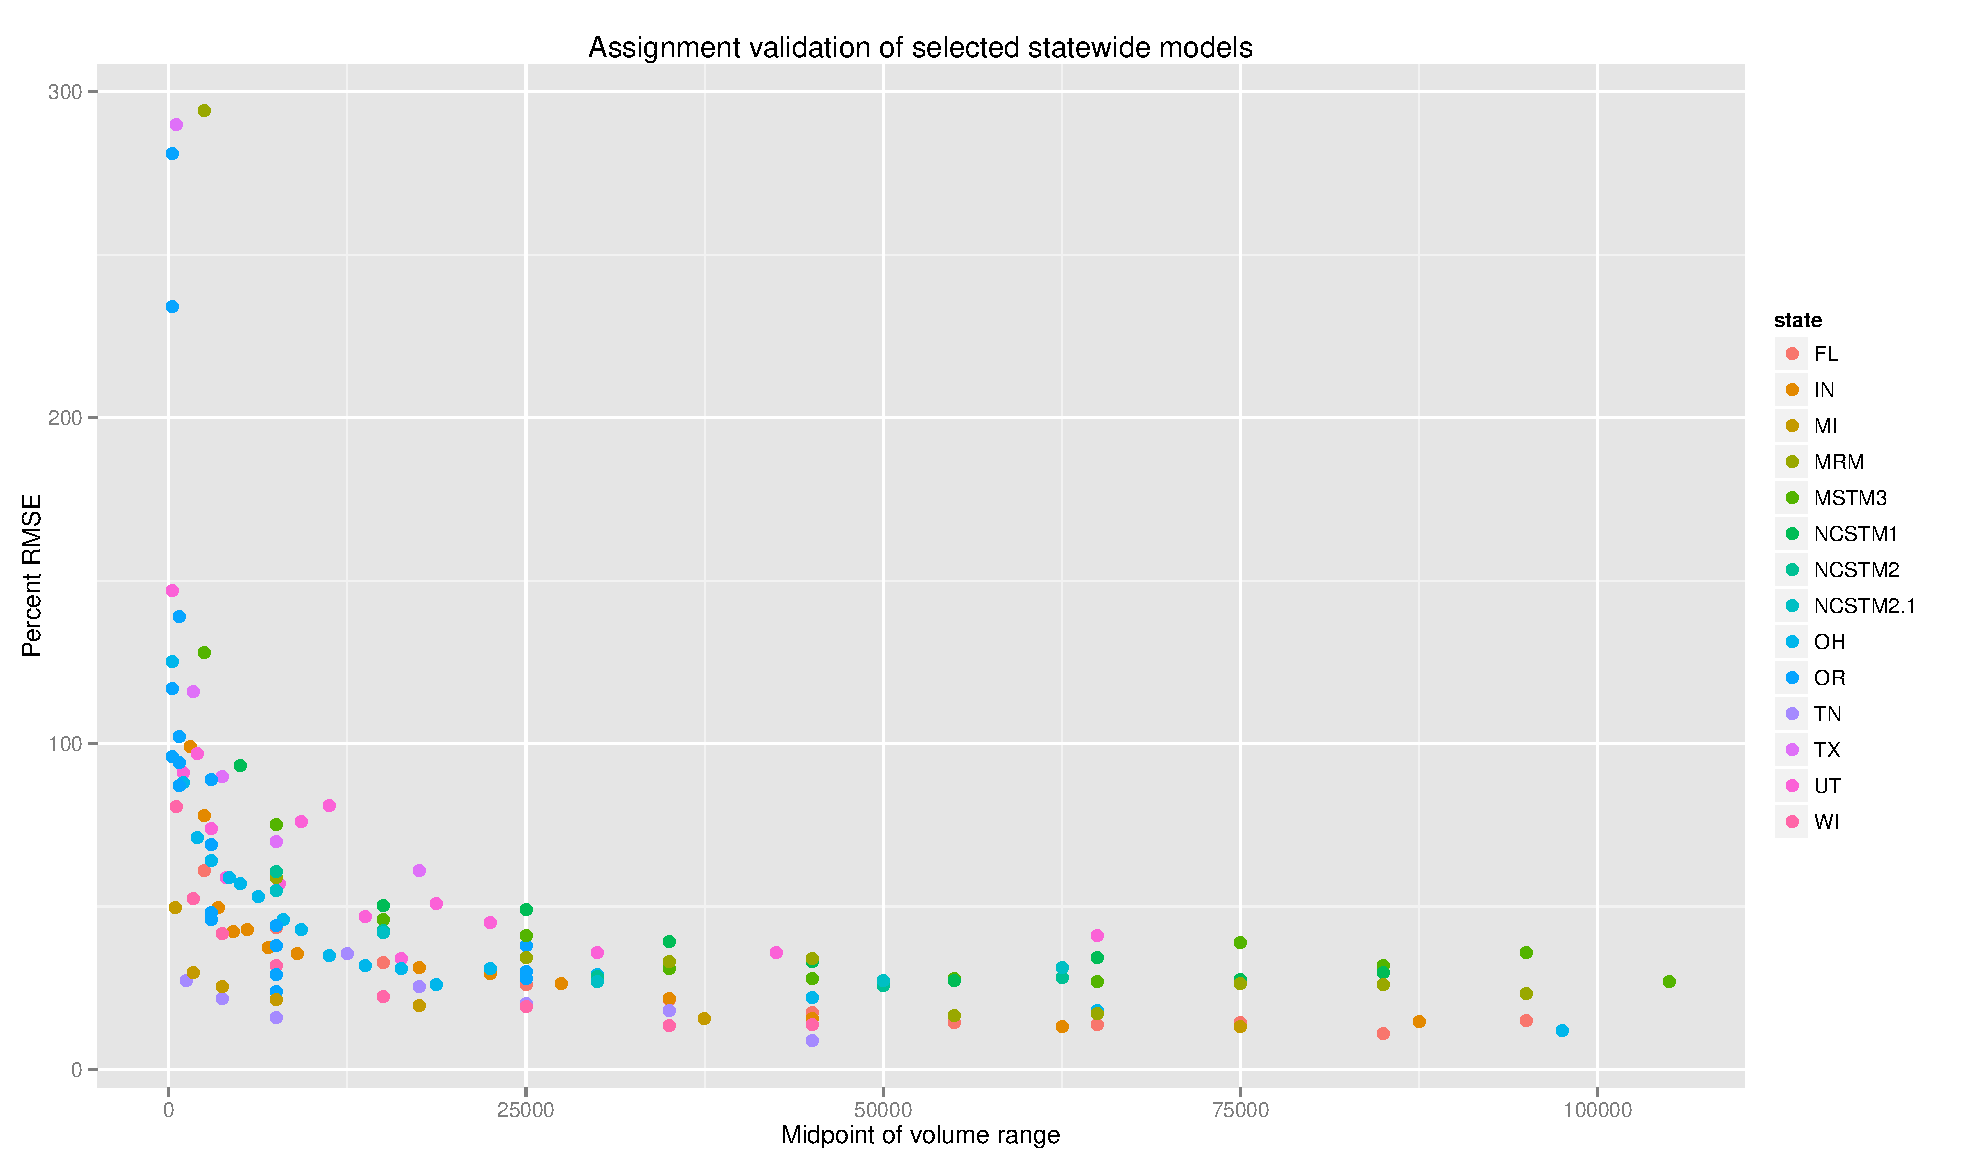
\includegraphics[width=6.5in]{graphics/47-prmse-comparisons}
\caption{Comparisons of percent RMSE by volume range for selected statewide models}
\label{fig:prmse-comparisons}
\end{figure}

\section{Computational burdens}

The 16-hour gold standard for statewide model runs --- the amount of time between when an analyst would start a run before leaving work and when they return to use its output the next morning --- is widely missed in many cases, especially those that cover large areas and populations, or have complex choice models. The urgency of addressing this issue was cited by several of the modelers encountered during the research for this report. This issue stems from a combination of factors:

\begin{itemize}
\item
The urge to build statewide models at the same levels of fidelity and resolution as urban models is strong. In some cases, this reflects the reductionist mindset of the model designer, but more often it is in response to needs to conduct fine-grained analyses of projects and corridors using statewide models. This need is particularly strong in areas of the state that are not covered by urban models, especially in corridors that connect two or more of them.
\item
The size of the state, both in land area and population, seems to correlate with the diversity and complexity of issues the models must be able to address. Thus, the already larger data and computational burdens imposed by the size of the networks and zone systems are compounded by more complex and complicated behavioral models.
\item
The overall trend in travel demand forecasting is towards a highly granular representation of agents and systems. Most advanced travel models work with synthetic households that are associated with much smaller zones than a decade ago, with the model operating on a continuous time scale or close to it. Some model the interaction between individual household members and their joint decisions. Such models are increasingly being coupled with dynamic traffic assignment models. Much of the evolving practice in urban travel modeling finds its way into statewide models, resulting in a slow creep of increasing detail in the latter.
\item
Advanced computational strategies remain out of reach for most model developers, whether they are using commercial software or not. No widely-accepted platform has emerged for the implementation of microsimulation-based advanced travel models, which are increasingly being used in statewide and urban modeling.
\end{itemize}

These realities leave statewide modelers with few choices for improving run-time performance, despite the frequent mention of the importance of improvements in this area. The lack of near-term options would seem to make this a modeling improvement priority.

\chapter{Case studies}\label{sec:case-studies}

Five case studies were selected to demonstrate typical implementations of statewide and megaregional models. However, standards for model application does not exist, as every implementation is unique and geared towards the needs of an individual state. Therefore, the case studies attempt to provide an overview of the breadth of statewide and megaregional modeling. These case studies include:

\begin{itemize}
\item
The Chesapeake megaregion model, which is the only operational megaregional travel demand model in the U.S. Even though it is not actively used now, it provides an intriguing example of large-scale modeling.
\item
The Arkansas statewide model employs a more traditional trip-based model that is an analog of the urban travel forecasting process. Being a smaller state, resources are more limited than in some larger states. Arkansas also provides an example of state-of-practice for integrating information from the FAF and external economic forecasts.
\item
The California statewide model is of interest for several reasons. The issues encountered while trying to integrate several quite different MPO models are worth describing. California also has notably ambitious carbon reduction targets that have affected model design. They have recently implemented findings from a household travel survey of approximately 44,000 households, making interesting discoveries.
\item
The Florida statewide model must deal with a geographically and socially diversity state and its forecasting needs. Florida has not only implemented a statewide model, but also urban modeling standards in conjunction with it, and interfaces between the two. Florida has also invested heavily in freight modeling, operating one of the most complex statewide freight models in the country.
\item
The Oregon statewide model is arguably the most complex and ambitious statewide model in use, making it well suited to represent the state-of-the-art in statewide modeling. Oregon operates an integrated economic/land use/transport/environment impact model designed to address issues most states do not address. The model has been under development over a decade, making it one of the more mature statewide models as well. This case study also provides an interesting illustration of the rationale and experience of investing in such a heavyweight model.
\end{itemize}

These case studies do not attempt to present the modeling system and supporting data in detail, but rather selected interesting archetypal aspects of every model are described. Readers interested in more details of these models are referred to the corresponding model documentations and user guides. This chapter aims to draw attention to the unique and exemplary details of each model, and document the breadth of approaches found in statewide and megaregional modeling.

\section{Chesapeake Bay Megaregion Model}\label{sec:chesapeake-bay-megaregion-model}

With the beginning of the 21st century, a revived interest in megaregions surfaced. Several research projects on the extent and relevance of megaregions were conducted, sponsored primarily by FHWA. Most notab:data-combinations is the book published by Catherine \cite{ross09a} on the delineation of megaregions across the U.S. Driven by her research, additional studies were conducted to explore the feasibility of modeling megaregional transportation systems. In 2010, FHWA commissioned a project to develop the first megaregional model in the U.S. to a team of Universities and Consultants let by the University of Maryland \citep{ducca13, moeckel15b}. One goal of this project was the development of a framework for a megaregion model that was tested in an implementation for the Chesapeake Bay Megaregion around Washington D.C.

The Chesapeake Bay Megaregion Model (CBM) for the Megaregion around Washington, D.C. is the only operational megaregional transportation model in the U.S. Arguably, there are other megaregional or quasi-megaregional models implemented elsewhere, such as \cite{gunn94} for the Netherlands and \cite{wegener08} for the European Union. However, no other complete travel demand model at the megaregional scale has been implemented in the U.S. \cite{zhang13} built a quasi-megaregional model for the Southern U.S. States, which was built to model traffic flows from evacuating the region if a hurricane is approaching. Thereupon, Zhang's model focuses on the assignment step, leaving out the travel demand side. The CBM remains the only operational megaregional model in the U.S. to date that includes all steps from travel demand to the assignment.

\subsection{Geography}

The CBM spans the area from the Southern border of Pennsylvania through Maryland and eastern Virginia to Norfolk and Virginia Beach. It includes all or part of five states: Pennsylvania, Maryland, Virginia, Delaware and West Virginia as well as the District of Columbia. The CBM is defined by its primary environmental resource, the Chesapeake Bay. Figure \ref{fig:chesapeake-bay-megaregion} provides a map of the CBM along with major surface transportation infrastructure.

\begin{figure}[!t]   % 48
\centering
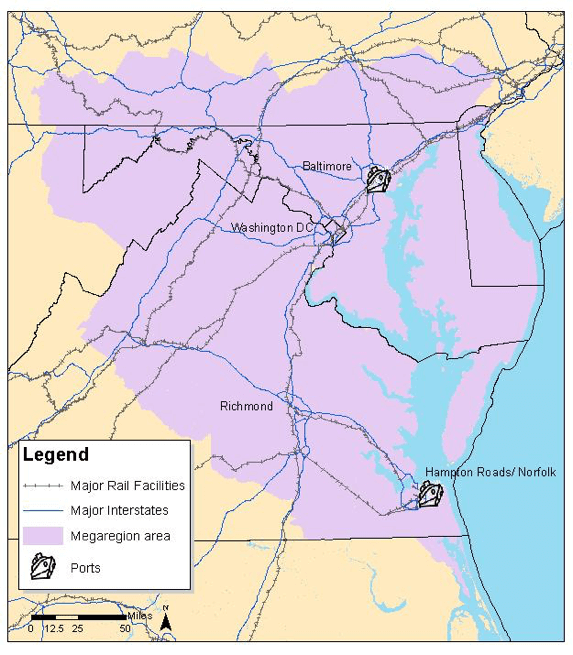
\includegraphics[scale=0.5]{graphics/48-chesapeake-bay-megaregion}
\caption{The Chesapeake Bay megaregion}
\label{fig:chesapeake-bay-megaregion}
\end{figure}

Given the geographic extent of a megaregion, a single scale model is insufficient to capture relevant activities, travel behavior, and their impacts. This fact is true for many statewide models as well, particularly if trips with external origins and destinations are modeled explicitly. Therefore, a two-layer approach was chosen to distinguish a megaregional layer represented in more detail and a national layer capturing relevant activities and flows outside of the main study area. Given the interactions between different megaregions nationally, and to some respect even globally, the two-layer approach facilitates to represent the study area with sufficient detail yet acknowledges that megaregions cannot be treated as monolithic islands.

\subsection{Model overview}\label{sec:cbm-model-overview}

The megaregion framework implemented for the CBM is shown in Figure \ref{fig:integrated-megaregion-model-concept}. A series of economic models predicts the growth and decline of different economic sectors based on assumptions of changes in the global economy. The economic models cover both the megaregional layer and the national layer to account for a global economy that affects growth and decline in the megaregion. The land-use model simulates changes in population and employment subject to this forecast.

\begin{figure}   % 49
\centering
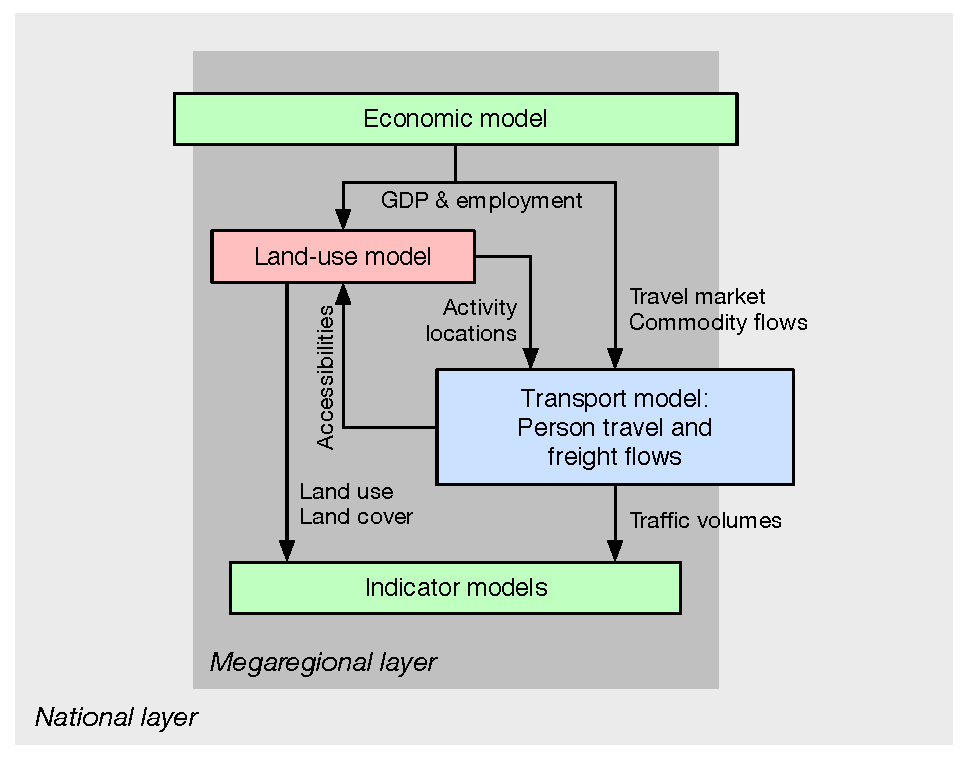
\includegraphics[scale=0.6]{graphics/49-integrated-megaregion-model-concept}
\caption{Concept of the CBM megaregion model}
\label{fig:integrated-megaregion-model-concept}
\end{figure}

The locations of population and employment are used in the travel demand model to simulate both person travel and freight flows. Accessibilities are fed back into the land-use model to influence land-use changes in the following simulation period, allowing land use to evolve over time. Finally, both traffic flows and the output of the land-use model are used in a series of indicator models to analyze the model results.

\subsubsection{Economic module}

To address the larger economic interest of a potential megaregion authority, the analysis framework emphasizes links with the economy, both nationally and locally. The megaregion model chain is driven by a national economic forecast component that predicts economic activity for large regions covering North America. The national Computable General Equilibrium (CGE) economic forecasting model built by the INFORUM group at the University of Maryland is applied \citep{mccarthy91}. The model employs inter-industry-macroeconomic general equilibrium models to examine past employment trends and to forecast future employment across 65 sectors of the economy. 

The primary model, LIFT (Long-term Inter-industry Forecasting Tool), uses econometric equations to predict final demand and output at the national level, based on inter-industry input-output relationships and value-added behavioral equations. The second component STEMS (State Employment Modeling System) allocates the national forecast to states, considering the industry's mix of basic and non-basic employment and personal income. Basic employment is driven by LIFT national industry trends, while non-basic employment is driven by state-specific personal income forecasts. The land use model further allocates these state control totals to model zones. Figure \ref{fig:county-level-flows} shows county level economic flows modeled for the CBM area.

\begin{figure} [!t]
\centering
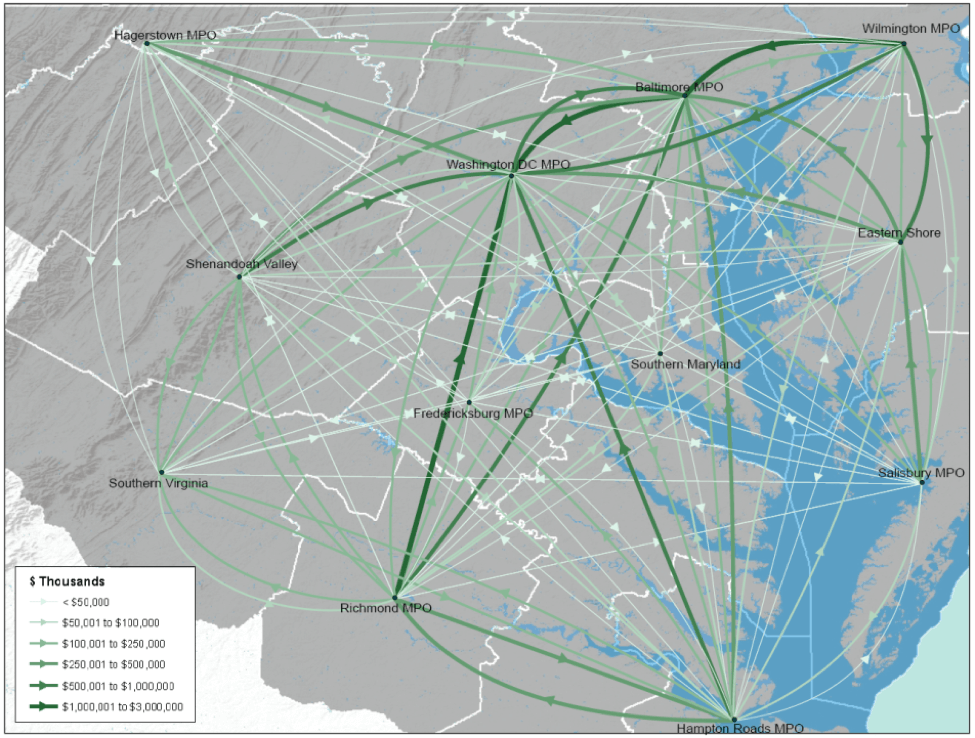
\includegraphics[width=6.5in]{graphics/50-county-level-flows}
\caption{County-level economic flows in the Chesapeake Megaregion}
\label{fig:county-level-flows}
\end{figure}

To account for local transport impacts on the regional economy beyond the national economic drivers that have little knowledge of local conditions, an economic post-processor was developed. The post-processor combines knowledge of county-to-county goods movement by industry and its sensitivity to travel impedance (generalized cost including time, distance, and travel cost per mile) to determine the impact of the local transport on each industry's supply chain relationships (up and downstream).

\subsubsection{Land use module}

The land use module works at two different geographies: a national geography with 126 zones covering North America and a megaregional geography with 2,075 zones. Economic flows generated by the economic model serve as control totals for the regional level:

\begin{itemize}
\item
  \emph{National Model:} Historic employment data from the U.S. Bureau of Labor Statistics Quarterly Census of Employment and Wages are disaggregated to counties. Employment data at the county level are used to calculate the share of employment in each county in the baseline years 2000, 2005 and 2009. The ratio of employment for each county is then extrapolated for five-year periods beginning in 2010 and ending in 2030 using an exponential smoothing method. Employment data from 101 BLS sub-sectors for the same period are then reconciled with 65 STEMS industries to match the BLS sub-sectors. This process simply employs a straight average of the two employment ratios. The purpose of this method is to allocate future STEMS projections based on the historic difference in BLS data and STEMS projections.
\item
\emph{Megaregional Model:} The local model generates socio-economic data at the resolution of megaregional modeling zones. The initial allocations are made based on transportation costs and the employment distribution of basic employment, or export-oriented employment. The allocation of households and employment is based on the Lowry model \citep{lowry64}.
\end{itemize}

The model is repeated in five-year increments until the horizon year 2030 is reached. The location of basic employment provides inertia in the allocation of non-basic employment. Obtaining data for a land use model at the scale of a megaregion is a challenging task, particularly if several states are involved. In contrast, a Lowry model requires less data but may provide reasonable land use sensitivities within computationally acceptable runtimes. Due to its simplicity and broad simplifications, the Lowry model has become rare at the urban level. At the megaregional level, however, such a model may provide the right balance between model sensitivities and comprehensiveness.

\subsubsection{Travel demand model}

Like the land use model, the travel demand model works at two geographic layers. While the local travel demand model is closer to a traditional statewide model, the national models are built from nationwide surveys for both personal and truck long-distance travel. Travel demand of the two layers is combined in the traffic assignment process that assigns short and long-distance traffic flows concurrently in a multi-class assignment.

The megaregional travel demand model is built as a five-step aggregate model that includes trip generation, destination choice, mode split, time-of-day split, and assignment. The original model concept was borrowed from the Baltimore Metropolitan Council model \citep{bmc07}, refined and applied for short-distance trips of 50 miles or less for the entire CBM study area. Trip generation rates were derived from a 2007 Household Travel Survey for the Baltimore and Washington D.C. metropolitan areas, as well as travel times, mode split and time-of-day split. Thereby, the model is calibrated to the core area of the CBM study area. A survey for the entire study area was not available.

This model includes a three-step local truck model based on the QRFM \citep{beagan07}, which was applied for local trips under 50 miles within the CBM study area. The comparison against VMT estimates revealed that the QRFM method, which is based on a 1992 truck trip survey from Phoenix, generated too many truck trips. Therefore, parameters were scaled down to resemble local VMT truck estimates and truck count data.

At the national layer, the National Estimate of Long-Distance Travel (NELDT) has been implemented to simulate long-distance person trips greater than 50 miles \citep{moeckel11}. The long-distance element of the 2002 National Household Travel Survey (NHTS), the most recent survey that covered explicitly long-distance trips in the U.S., provided data input. To expand the survey to cover all long-distance trips in the U.S., air travel data from the Bureau of Transportation Statistics (BTS), which covers 10 percent of all ticketed air travel passengers, was used as a control total to scale NHTS records to observed flight volumes. Auto trips were generated using the same scaling factor and added to the multi-class assignment with local traffic.

For freight long-distance travel, commodity flows from the Freight Analysis Framework FAF3 were used for truck trips of 50 miles or more. Though the 123 FAF zones reflect centers of economic activity, the resolution is too coarse to model truck trips on a network with much more detail. Therefore, flows between FAF regions were first disaggregated to flows between counties and then further disaggregated to flows between model zones. To disaggregate commodity flows, make/use coefficients and employment by type were used to allocate flows to the most likely producers and consumers of every commodity.

Commodity flows between zones are converted into trucks trips using average payload factors provided by FAF. These factors describe how many tons of a given commodity are carried by a truck on average. To account for empty truck trips, an empty-truck trips rate was added globally to all truck trips.

\subsubsection{Environmental and fiscal impacts}

A few indicator models were added to estimate the environmental and fiscal impacts. The results of the indicator models are not fed back to the other model components but were used to evaluate scenarios:
\begin{itemize}
\item
\emph{Gaseous Emissions:} This model captures traffic emissions using the EPA Motor Vehicle Emission Simulator (MOVES) model (EPA 2016). The MOVES model uses VMT and link-level volumes and speed data output of the travel model to estimate GHG and other mobile emissions.
\item
\emph{Water Quality:} This model captures the impact of alternative policies on water quality. A nutrient-loading model estimated flows draining into the Chesapeake Bay. It forecasts the annual loads of nitrogen, phosphorus, and sediments. The model uses detailed land cover changes from a raster-based land use model to identify changes in nutrient runoff due to land cover changes.
\item
\emph{Infrastructure Costs:} This model estimates state and local governments' costs to provide public infrastructure in support of new development (e.g. roads, sewer, water). Established relationships between the current development and the provision of infrastructure were applied to project future improvements needed to satisfy additional settlement activity. Data included residential development classified by housing type, existing water and road infrastructure, property value trends and tax rates, among others.
\end{itemize}

\subsection{Lessons learned from the CBM model}

The design of the CBM model is similar to a statewide model. A comparable two-layer geography is represented in many statewide models to distinguish long-distance and short-distance travel. Special attention was given to add additional model components, such as economic, land use as well as environment and fiscal impact models, though many other statewide models use such ``add-ons'' as well. A significant challenge for the CBM was a study area that included parts of five different states and the District of Columbia.

While many statewide models cover parts of neighboring states at a higher resolution, it is rare that data from as many states are included. Creating a network from different sources, socio-economic data from different agencies and count data in different formats created a challenge for the development of the CBM. As such, the model was operational but only implemented as a prototype. Detailed model validation has never been conducted outside of Maryland.

As with many statewide models, the CBM coped with two levels of model integration (Figure \ref{fig:horizontal-vertical-integration}). On the one hand, vertical integration covers the interaction between different geographies, here the North America level with the megaregional level. On the other hand, horizontal integration captures the interaction between different modeling domains, such as transport models with land use models. A core finding was that the level of integration depends on (a) the frequency of information exchange, (b) the direction (one-way or bi-directional) and (c) software implementation constraints. Tighter integration turned out to not always be better. In some cases, lose coupling of models may be sufficient and much easier to implement.

\begin{figure}
\centering
\includegraphics[scale=0.6]{graphics/51-horizontal-vertical-integration}
\caption{Horizontal and vertical integration in a megaregional model}
\label{fig:horizontal-vertical-integration}
\end{figure}

The work resulted in an extensive report \citep{ducca13} and a paper published \citep{moeckel15b}, but was never used as a true policy advice tool. Being funded by FHWA's Exploratory Advanced Research Program, it was not expected to be applied in practice. However, the work has not inspired the development of other megaregional models yet. Most likely, this is due to the lack of megaregional institutions across the U.S. that might use large-scale models to advise decision making. Therefore, the CBM model remains a proof of concept that may assist other megaregions in the future.

\section{Arkansas Statewide Model}

The Arkansas State Highway and Transportation Department (AHTD) completed a Phase II update of their statewide model in 2015. All parts of the model and underlying data were addressing during the update. The resulting modeling system represents an excellent example of best practices in statewide modeling, incorporating current thinking about how such models might evolve in the future. These qualities are shared by other models reviewed in this chapter. What makes Arkansas unique, however, is that they could leverage prior work and experience to do so within modest budget, and their creative approach to overcoming a lack of local travel behavior data.

A multi-scale modeling approach was employed to develop a model that provided a regional and national context for Arkansas, while still providing a high enough level of detail for accurate forecasting of policy and project scenarios within the state. The state is covered by 5,849 traffic analysis zones, designed to include urban model zones as already defined, and to be compatible with and nest within Census block and block group boundaries otherwise. Care was also taken to respect natural boundaries that impede flow, as well as not crossing major roadways and highways.

The rest of North America is covered by 144 zones formed by aggregations of Economic Areas defined by the Bureau of Economic Analysis (U.S. Department of Commerce) with the USA, and states and provinces within Mexico and Canada. Like many other statewide models, urban model networks within the state are fused with the FHWA National Highway Planning Network to represent the roadway system. A rail network maintained by Oak Ridge National Laboratory was used to represent the freight rail system.

Their model is described next, followed by a discussion of their innovative approach to data development and lessons they appear to have learned. Their model documentation, spread across eight reports, is available upon request from AHTD.

\subsection{Long-distance freight models}

Long-distance truck and rail flow forecasts are developed using four-step sequential modeling process, based upon commodity flow forecasts. Their model is based upon a 2008 Global Insight Transearch flow database. Unlike many states, who map the flows to truckload equivalents, the data are used to build a commodity flow model. This provides a degree of policy sensitivity that static forecasts, such as the Transearch and FAF static forecasts, do not. In this case changes in employment can be used as a proxy for changes in gross state product, growth in certain industries relative to others, and the like.

Linear regression models are used to predict annual tons shipped by all modes of transportation as a function of employment within industries that produce such goods, for 15 commodity groups. The production model was estimated at the county level within Arkansas, and state level outside of it, for 13 of those groups (reported flows in the Transearch data were used for mining and coal flows). The resulting r\textsuperscript{2} statistics ranged between 0.46 and 0.84, providing reasonable fits, Attraction models were likewise estimated using linear regression, using input-output tables to understand better the linkage between commodities and consumption. Special generators were developed for counties whose actual tonnage (from the Transearch data) deviated significantly from the regression estimates.

A doubly-constrained gravity model is used for trip distribution, using friction factors based on the distances coded in the Transearch data. The latter are often used instead of mathematical functions to replicate the multiple peaks in observed trip distance distributions. An incremental mode choice model, based upon existing mode shares by commodity and distance ranges, was developed using the Transearch data. The rail tonnage was assigned directly, with truck tonnage converted into daily truckload equivalents using payload and annualization factors. The latter were combined with auto flows in a multi-class traffic assignment.

\subsection{Person and other truck models}

Person local and external travel, as well as non-freight commercial vehicles, are modeled using the widely-accepted trip-based modeling paradigm, with a few interesting extensions. A schematic diagram of the modeling system is shown in Figure \ref{fig:arkansas-flowchart}. Nine person and four truck trip purposes are modeled, to include two of each devoted to external trips (i.e., those crossing the state border). Two of the purposes represent infrequent long-distance travel, which includes trips longer than 100 miles. Like an increasing number of states, person trip generation rates are differentiated by area types (four in this case, as a function of population and employment density) in addition to household size and income groups. Attraction rates were calculated using borrowed data, stratified by the same four area types and income groups, as well as total households and employment by broad categories. Special generator attractions were calculated for unique land use types, such as universities, hospitals, military bases, and airports.

\begin{figure}[!t]
\centering
\includegraphics[scale=0.6]{graphics/52-arkansas-flowchart}
\caption[Schematic diagram of Arkansas statewide model]{Schematic diagram of Arkansas statewide model (Source: \cite{alliance15}}
\label{fig:arkansas-flowchart}
\end{figure}

Doubly-constrained gravity models are used for trip distribution, using distance as the measure of impedance for infrequent long distance trips, and travel time for all other trip purposes. Friction factors were fitted to smoothed trip length frequency distributions for each trip purpose, and iteratively calibrated to survey data. A nested logit mode choice model that handles both local and intercity travel was developed, based heavily upon Federal Transit Administration (FTA) guidance and typical practices. Several of the model coefficients were asserted, based upon FTA advice, and then calibrated to local conditions. Calibration targets were generated from 2009 NHTS data for auto trips, while data from two Arkansas transit agencies were used for transit trips. The daily person trips by mode were allocated to four periods of the day, using diurnal factors by trip purpose and direction. Finally, the person flows were converted into vehicle trips through the application of auto occupancy rates, where appropriate.

External trips are those with an origin, and possibly destination as well, outside of Arkansas. This corresponds to the familiar external-internal (EI) and external-external (EE, or through) trip purposes. Because both local and long-distance trips by Arkansas residents are modeled there is no need to include internal-external (IE) trips, for they are already accounted for within the modeling steps described above. Traffic and vehicle classification counts at the state border are used to constrain the flows to observed or forecasted levels. The external trips go through the same diurnal factoring as internal trips before being combined with them for traffic assignment.

The person travel models include truck flows that are not represented in the Transearch data described above. These include trucks making local trips, as well as non-freight trucks traveling over longer distances. They are modeled in a similar manner as persons, using data borrowed from Idaho. Regression models by truck type were developed for trip generation, which are assumed to also represent trip attractions. Trip distribution models like those developed for person trips were calibrated for three categories of trucks. Diurnal factors were borrowed from Idaho, and compared to those found in the literature and other statewide models. When combined with the long-distance truck trips described in the previous section these flows represent the entire population of trucks operating within Arkansas.

\subsection{Traffic assignment}

The Arkansas model includes both highway and freight rail assignment procedures. The former is carried out for four time periods and includes feedback loops to obtain more accurate travel times, as shown in Figure \ref{fig:arkansas-flowchart}. Several user classes are jointly assigned. Trip matrices are segmented by 18 combinations of trip purpose, auto occupancy, and income groups to define the user classes. This is more detail than thought to be used in most statewide models. A multi-class static user equilibrium assignment process is run separately for four periods of the day, with each converging through feedback separately.

The widely-used Bureau of Public Roads (BPR) volume-delay function is used to update link travel times during assignment. The model coefficients were updated in the Arkansas model, drawing upon experience in other states and the literature. Ten variants are used to capture differences in perceptions and values within each user class. The function coefficients are also segmented not only by functional class, but by whether the downstream node is a signal or stop sign controlled, or not an intersection. Considerable effort apparently went into derivation and testing of these coefficients, as well as sensitivity testing of toll costs.

A simpler assignment process was also developed, to be used to reduce the computational burden and data handling associated with a large number of user classes. Three user classes (passenger, commercial trucks, and heavy trucks) are used, although doing so precludes analyses of toll and high-occupancy lanes. The modeling system also includes the capability to assign freight rail tonnage or annual train equivalents on a simplified rail network. The origin-destination flows are assigned to the shortest distance path, rather than attempting to capture the complexity of rail routing decisions that include factors such as interlining cost, track ownership, and cost minimization. The goal is to visualize the spatial dimensions of rail traffic, not its exact routing, for which their method is quite adequate.

\subsection{Innovative data development}

The developers of the Arkansas model had to overcome several data shortcomings, with the lack of household and truck travel survey being the most significant. It is common in such cases to borrow or assert models, or synthesize them using data from different sources, and to calibrate the model to what local data are available. Like other states, the developers turned to the NHTS for this task. However, there are too few observations within Arkansas to build a statistically stable and reliable with. However, both Tennessee and Texas had purchased additional samples during the 2009 NHTS cycle, which proved invaluable for the development of the Arkansas model. Summaries from both states were compared during each step of the person travel model. The Texas data were used in each case, for their much larger sample size (22,255 households) was an order of magnitude larger than collected in Tennessee. However, the differences between them, as well as summaries of the small samples from other nearby states and 2003 household survey from Central Arkansas, defined the range of such values. This helped identify which patterns and relationships were the most stable, versus those where Arkansas would likely vary from its neighbors.

Similar data were borrowed for other parts of the model, to include:
\begin{itemize}
\item
Workplace surveys from Arkansas were similarly not available. The team obtained permission to use data from four Texas workplace surveys to develop trip attraction rates. The resulting rates compared well to other models and the literature.
\item
Typical mode choice model structures, parameters, and coefficients were drawn from FTA New Starts guidance, as well as advice from senior modelers in the agency. The collection of onboard travel survey data, coding and testing of transit networks, and formal estimation of parameter estimates is very time-consuming, and of questionable value in settings like these. Synthesizing these data saved the developers considerable time, permitting them to focus more time on calibration and sensitivity testing, both of which led to better modeling outcomes.
\item
Data from a 2008 commercial vehicle survey conducted for the Community Planning Association of Southwest Idaho (COMPASS), the MPO for the Boise area, were used to develop the truck characteristics in the person travel model (e.g., those trucks not included in the Transearch data, to include local and non-freight truck movements). These data proved invaluable for the development of that part of the model.
\item
Experiences with traffic assignment models, to include volume-delay function parameters, were heavily informed by models implemented in several other states by the developers.
\end{itemize}

The effective use of these data reduced both the cost and time required to develop the Arkansas model. Judging from the reported validation statistics, these borrowed data enabled the model to perform as accurately as reported in many other states. Thus, Arkansas has a fully functional model, when they might still be in development stages had they invested in a large-scale household survey across the state. In a sense, the availability of these data has made statewide modeling affordable for Arkansas, and therefore accessible when it might not otherwise have been.

\subsection{Lessons learned from Arkansas}

Arkansas is a relative newcomer to statewide modeling, having first embarked upon its first version in 2010, and recently updating it. They achieved this through leveraging work done elsewhere, as well as learning from their experience. Some of the more important and interesting successes include:

\begin{itemize}
\item
The NHTS is a very important resource for statewide modelers, for many states lack the resources required to conduct statewide travel surveys. However, little has been done to compare how estimates for one state stack up against its neighbors, or whether data from several states can be pooled in to gain acceptable sample sizes. Several developers have already done so, of course, but few compare the results in each step of the model like Arkansas has done. This underscores the importance of funding add-on surveys (i.e., paying for the collection of additional surveys) in future versions of the NHTS for those states unable to conduct such surveys on their own, as well suggesting the value of several adjacent states pooling funds to do so.
\item
Considerable work went into the development of a graphical user interface and standardized reporting, both of which make the system and its outputs more accessible to both modelers and their clients. Having a model that is easier to use enables AHTD staff to spend more time evaluating results, rather than setting up and running the model in an ad hoc manner.
\item
The focus was on the usability of the model throughout its development. This not only drove the initial design, but remained in focus when evaluating validation outcomes and deciding upon changes and possible model enhancements. This is best illustrated in their adoption of FTA guidance and advice in the construction of their mode choice model. Rather than developing a model and testing its utility, the developers started with a recommended approach and worked backward to determine how best to calibrate and test it. This approach saved considerable time and effort for a part of the modeling system that is often as costly as the rest combined.
\end{itemize}

Their current model appears capable of meeting their short-term needs, and represents a sound investment. How the model will evolve over time to address new and more complex issues not well addressed using trip-based modeling systems remains an open question. There is no doubt, however, that Arkansas is on a path that will enable them to do so in a highly cost-effective manner.

\section{California statewide models}\label{sec:ca-statewide-models}

On paper, California has the most expensive statewide model in existence, by a wide margin. While it is difficult to pinpoint the full cost of statewide modeling, the costs shown in Figure \ref{fig:resource-allocation} (page \pageref{fig:resource-allocation}) suggests that their costs far exceed those of other states. A closer look reveals that their program involves far more than just statewide travel modeling, and forward-thinking and ambitious investment in data collection that eclipses those of almost all other states. Moreover, there are two statewide models of California, which unto itself is an interesting story. Their modeling systems and what they can do with them, how they have partnered with others in their development, and how they might complement one another are described in this section.

Extensive and current documentation about both modeling systems is available online. These include descriptions of the models and their development, as well as reports about supporting data, results of model testing, forecasts developed using them. In the case of their HSR model the findings of an independent peer review panel are also published on the Authority's website. This might not seem remarkable today, until one attempts to find similar documentation for most other statewide models online. Viewed in that light, California is commendably progressive in making extensive documentation of their statewide travel data and models publicly accessible.

Each modeling system is described in the following sections, with a focus upon the unique and noteworthy aspects of each.

\subsection{The California Statewide Travel Demand Model}

The California Department of Transportation (Caltrans) has developed a comprehensive multimodal statewide model of all personal and commercial travel by residents of the state. The model system is used by Caltrans for a variety of analyses. The system was designed to meet several analytical needs:

\begin{itemize}
\item Provide insights into long-distance travel between and through multiple regions of the state
\item Model behavior for all California residents and firms, expressed as multimodal tours and trips
\item Provide data on external travel for urban and metropolitan travel forecasting models
\item Evaluate changes in greenhouse gas emissions, as required by several state laws
\item Provide aggregate travel statistics that can be used to resolve differences between adjacent urban and regional models
\item Provide a travel demand model for agencies that do not maintain a model of their own
\end{itemize}

Descriptions of the modeling system and data, as well as how they have partnered with other agencies, are presented in the next sections.

\subsubsection{Partnerships}

Caltrans has partnered with several agencies to fund and direct their statewide data and modeling program. The first-generation model was funded through university research, as is work on a new freight modeling framework. Their recent statewide travel survey, described below, was designed to collect data needed for both transportation and environmental models. The list of collaborators is impressive, and is unmatched by any other state except Oregon:

\begin{itemize}
\item California Air Resources Board
\item California Strategic Growth Council
\item California Department of Public Health
\item California Department of Housing and Community Development
\item California Energy Commission
\item California High-Speed Rail Authority
\item Metropolitan planning organizations
\item Regional transportation planning agencies
\end{itemize}

Not all partners are involved at the same level, but the statewide modeling program in California has greatly benefited, and had more resources at their disposal as a result. Granted, California has passed legislation requiring such collaboration to achieve sustainable planning and greenhouse gas reduction targets. Specific multi-agency mandates and deadlines are required in several laws, to include:

\begin{itemize}
\item California Global Warming Solutions Act (AB 32, passed in 2006)
\item Sustainable Communities and Climate Protection Act (SB 375, passed in 2008)
\item California Homes and Job Act (SB 391, passed in 2013)
\end{itemize}

Regardless of the motivations, the level of inter-agency cooperation and pooling of resources to solve large problems is helping to drive the agenda for statewide modeling, both directly and indirectly.

\subsubsection{Data development}

Many agencies rely on the NHTS or data borrowed from other areas to build their statewide models, as revealed in Table \ref{tab:data-combinations} (page \pageref{tab:data-combinations}). California, like a few other states, has opted instead to collect the data it feels are required for robust models. Some have no parallel in other places, and have enabled Caltrans to develop the advanced model that it currently uses. Two of the most important recent data collection activities
included:

\begin{itemize}
\item
The 2013-14 California Household Travel Survey (CHTS) collected data from households in all California counties, and three in Nevada \citep{nustats13}. A traditional 24-hour travel diary was used to record trips by all modes of transportation for all respondents, and in some cases, three types of GPS data collection (wearable, in-vehicle, and connected to the on-board diagnostics {[}OBD{]} port). Data were collected from the GPS units for periods of three or seven days, depending upon the device used. Households were also asked to also report long-distance travel over the past eight weeks using a separate retrospective survey. Complete data from a total of 42,431 households were collected, to include 5,717 from which GPS data were obtained. An additional dataset of partially completed surveys for 20,651 households was provided, which some of the survey sponsors considered still useful.
\item
The 2014 California Vehicle Inventory and Use Survey (Cal-VIUS) is designed to fill the gap left by the cancellation of the federal survey a decade ago. Like its national predecessor, they survey is designed to collect data on the physical and operational characteristics for a sample of all commercial vehicles. The survey, being conducted by the Institute of Transportation Studies at the University of California-Irvine, is being conducted in two parts. The first is a web-based survey of fleet managers, used to collect information about the vehicle and its annual operation. A driver survey is completed from a mobile phone app over a three-day period. These data will be invaluable for developing and validating the commercial vehicle models. The survey is currently in progress.
\end{itemize}

\subsubsection{Overview of the modeling system}

The second version of the California Statewide Travel Demand Model (CSTDM) was delivered in 2014 (Cambridge Systematics 2014). It is a multimodal, tour-based travel modeling system with five major components, as shown in Figure \ref{fig:cstdm2-structure}. All the models employ a microsimulation framework, in whole or in part. The SDCVM, for example, uses aggregate models to generate tours, and microsimulation to add their attributes. The system simulates travel by all California residents and firms, for a typical weekday in the fall or spring. Databases have been developed to support forecasts for 2015, 2020, 2035, 2040, and 2050. In a nutshell, the five components include:

\begin{figure}  % 53
\centering
\includegraphics[scale=0.6]{graphics/53-cstdm2-structure}
\caption{Structure of the California statewide travel demand model}
\label{fig:cstdm2-structure}
\end{figure}

\begin{itemize}
\item
The SDPTM consists of a series of logit models that generates tours and trips by five periods of the day. Starting from a synthetic population, long-term choices are modeled first, to include work and school location and driver license status. Daily tours are then generated, as well as their primary destination and mode of travel. Secondary destinations are then chosen, followed by trip mode choice. The models are applied somewhat differently for each tour purpose.
\item
The LDPTM is based upon the approach used in the statewide HSR model, which begins with a tour formation model. It is run in parallel with the SDPTM. Tour attributes are then generated, with models of party formation (size), tour properties (duration and time of day), destination choice, and mode choice. The latter includes main, access, and egress choice models, based upon an earlier version of the HSR long-distance mode choice model. An interesting aspect is how both models interact, as shown in Figure \ref{fig:california-interactions}.
\item
  The SDCVM is an adaptation of a tour-based microsimulation of CV flows, based on a model originally developed in Calgary \citep{hunt07}, and based upon parameter values from its implementations in Alberta and establishment survey of California businesses. The model structure is illustrated in Figure \ref{fig:calgary-model}, which simulates flows from six categories of establishments, for three types of trucks.
\item
The LDCVM is based upon truck origin-destination flows derived from a PECAS model implemented in the first-generation statewide model. Growth factors are used factor the trip matrices for future years, based upon growth in zone-level demographics. While the original flows were developed using PECAS, the current model does not depend upon it for current or future forecasts.
\item
The ETM models handle flows to and from 51 external stations in the model, including three marine ports. They are organized into six districts across the state. Existing counts at the external stations, and extrapolations into the future, are used to generate external trips. A logit-based destination choice model is used, and trips are allocated to time periods using observed patterns.
\end{itemize}

\begin{figure}  % 54
\centering
\includegraphics[scale=0.6]{graphics/54-sdptm-ldptm-integration}
\caption{Integration of the California short and long-distance person travel models}
\label{fig:california-interactions}
\end{figure}

\begin{figure}   % 55
\centering
\includegraphics[width=6in]{graphics/55-calgary-model}
\caption{Structure of the Calgary commercial vehicle model}
\label{fig:calgary-model}
\end{figure}

The resulting modeling system includes 5,474 traffic analysis zones, which nest within California counties and 524 land use zones used by the PECAS model \citep{hunt05}. The latter was an integral part of the first-generation statewide model, but is not an active part of the current version. The network includes over 325,000 nodes, including its sparse representation of the national Interstate and US highway system.

One innovative feature is the use of a simplified representation of local transit service, using a technique described by \cite{circella13}. Fixed guideway and intercity transit lines are explicitly represented in the model, but the level of service times and costs are synthesized based upon roadway speeds, land use variables, and assumptions about transit service levels. The same methodology is used in the Oregon statewide model, to obtain reasonable approximations of local transit accessibility without the huge effort required to code every local bus line within the state.

\subsubsection{Next steps}

Caltrans plans to complete model updates on a five-year basis, incorporating data that has become available or been updated since the last update. Caltrans is sponsoring the development of a new multimodal freight model that will eventually replace the long and short-distance commercial vehicle models in the current system. Both steering committees and peer review panels will be used to provide advice about the long-term evolution of the statewide model and its supporting data programs.

\subsection{The California High-Speed Rail Ridership and Revenue Model}\label{sec:california-hsr-model}

The California High-Speed Rail Authority maintains a separate ridership forecasting model, used to support business and system planning, as well as corridor studies and analysis of alternative alignments and phasing of implementation. It is a complete statewide model, and uses some of the same data used to develop the Caltrans model. It incorporates a more sophisticated mode choice model better suited for evaluating HSR alternatives, but otherwise covers the same travel markets as the Caltrans model, and at comparable levels of spatial, temporal, and behavioral resolution. It also includes an explicit risk and uncertainty assessment process. This is a necessity for HSR forecasting, but unfortunately unique among the statewide models reviewed for this report.

The Authority oversees the ridership forecasting work, with assistance from their Rail Delivery Partner (RDP) and an independent peer review panel. However, all model development and application work has been undertaken by Cambridge Systematics, under contract to the RDP. The associated cost of developing and using this model is not published, but is thought to be comparable to the investment made in the Caltrans model and data. Moreover, scores of forecasts have been produced with it. Because these were undertaken by the consultant those costs likely account for a significant portion of the total cost incurred by the Authority.

Several aspects of the California HSR model and how it is used are noteworthy. A summary of their modeling system, as well as data and institutional aspects of its development and deployment, are described in the following sections.

\subsubsection{Open and transparent analytics}

The California HSR model is unique in several aspects, both in comparison to other HSR forecasting efforts and most other statewide models. Most HSR forecasts, both domestically and abroad, have been undertaken by consultants that use proprietary models and data to develop them. The overall approach is described in their reports, as well as characterization of major market trends driving the trajectory of the model. Narrative, tabular, and graphical summaries of the forecasts are also provided, along with their interpretation. However, the forecasts are the delivered product, not the data or models used to develop them. This precludes reuse of the data and models, as well as detailed review and testing. California breaks from that tradition, having developed the data and platform used for their analyses. This gives them the ability to test new alternatives quickly, as well as generating new forecasts to reflect changing alignment, service levels, fares, etc. It should be transferable to other regions, although no known attempt has been made to do so.

The model was originally developed under contract to the Metropolitan Transportation Commission in the Bay Area. It was based, in part, upon results from stated preference surveys carried out in 2005 within the state and older statewide travel survey data. It was subsequently extended to support statewide analyses for the Authority, and updated with new data and models. The current version of the system, known as the Business Plan Model-V3 (BPM-V3) incorporated new survey data from the CHTS and a 2013-14 SP survey performed for the Authority, a completely revised mode choice model, and improvements to almost all the other modules.

The model is extensively documented (Cambridge Systematics 2016a), as are the data used to develop and apply it. Documentation about the model structure, key parameter values and their derivation, and tests of the effect of major assumptions are available on the Authority's website.

\subsubsection{Data development}

An intercept survey of stated and revealed intercity mode preferences of California residents was undertaken in 2013-14. Data about respondent attitudes towards, and experience with, HSR elsewhere were also collected. The data, and how they compared to results obtained in an earlier survey completed in 2005, were used to develop a new mode choice model (Cambridge Systematics et al. 2015). The stated preference (SP) portion consisted of six experiments presented to each respondent, consisting of several options for mode of transport and variations on important characteristics of each. A total of 4,314 respondents provided complete and usable data. About 40 percent were from conventional rail riders, while the remainder were split almost evenly between air and auto travelers.

The results of the CHTS, and particularly the long-distance element, were also used in model estimation and calibration. The daily diary portion of the survey was large enough to accurately portray the incidence of long-distance travel on the survey day, something smaller surveys struggle to capture. While the number of such observations was too small to build robust models, the CHTS travel diaries did prove useful for validating the incidence of long-distance travel. Information about the latter was also gleaned from an additional eight-week recall survey of long-distance travel. This optional part of the CHTS provided data on 32,641 long-distance trips by California residents, which was used for some parts of model development, and validation of other parts. The aggregate results were also adjusted based on 2011 data from a Harris Panel survey, to understand gaps in the data, particularly with respect to uncertainty about how CHTS respondents reported repetitive trips.

\subsubsection{Bi-level modeling framework}

The modeling system employs the bi-level structure shown in Figure \ref{fig:bpm-v3}. The long-distance model includes trips within the state longer than 50 miles, stratified by four trip purposes. They include business, commuting, recreational, and all other trips, a common scheme used in long-distance travel models. The trip frequency and destination choice models were estimated using the CHTS long-distance survey data and revealed preference (RP) portion of the 2005 RP/SP survey. The mode choice model is a combined model of main, access, and egress mode choice, estimated from the weighted RP/SP surveys alone. Several nesting structures were tested, and the final model was calibrated using the expanded CHTS, rail boardings, and air travel flow data.

\begin{figure}   % 56
\centering
\includegraphics[scale=0.575]{graphics/56-bpm-v3}
\caption{Structure of the California HSR Business Plan Model-V3}
\label{fig:bpm-v3}
\end{figure}

The short distance model includes person trip tables by mode and trip purpose from the regional travel models used by the Southern California Association of Governments (SCAG) and the Metropolitan Transportation Commission (MTC). They are the metropolitan planning organizations for the Los Angeles Basin and San Francisco Bay Areas, respectively. Trip tables for their base and forecast years are used to represent short-distance travel within the BPM-V3 framework, and are translated into the format required by the short distance mode choice model.

The mode choice model is an adaptation of the 1996 Baycast model developed for MTC, which has been calibrated to reproduce base year transit ridership within each metropolitan area. More recent models in both regions are further apart in structure, precluding their direct use within the BPM-V3 framework. The resulting system provides consistent forecasts of short-distance mode choice within both regions. The station spacing outside of those regions is too far apart to enable short-distance HSR trips, obviating the need for short-distance models within the rest of the state.

The BPM-V3 system and its predecessors have been used to generate ridership and revenue estimates for initial and detailed system planning and in support of corridor studies and evaluation of candidate initial operating segments. This has included the environmental studies required at all levels of analyses for the program, and use for station-level impact analyses. The latter has required post-processing of the model outputs, for the model was not designed to support detailed analyses at a fine level of geography. The SCAG and MTC models are well-suited for that level of analyses, but only for station-level analyses within their modeled area. 

The BPM-V3 and its predecessors have also been used to generate forecasts for the Authority's biennial business plan. The process used to develop the forecasts and their interpretation is described by \cite{cambridge16b}.

\subsubsection{Independent peer review}

The early forecasts developed using the first version of the model were heavily criticized with respect to their derivation and accuracy \citep{brownstone10}. The Authority formed an independent peer review panel of prominent experts in travel demand forecasting to review the entire modeling system, not just those parts at controversy, and advise the Authority on its fitness for use. The Panel conducted a thorough review over a period of several months, and made several recommendations that guided the development of the second and third versions of the modeling system.

The group was renamed the Ridership Technical Advisory Committee in 2014, as their role changed from the independent review of the original model to providing advice to the Authority on long-term goals for their forecasting work, review of interim products, and continued review of technical aspects of the modeling system. Their work and findings are reported in over a dozen reports published on the Authority's website.

\subsection{Lessons learned from California}

Several regulatory and policy issues seemingly unique to California have influenced how their statewide models have evolved. However, climate change, economic interaction, sustainability, and new technologies are issues that other states are beginning to grapple with as well. Some of the key lessons learned from California include:

\begin{itemize}
\item
The importance of, and value gained from, data collection cannot be overstated. California has invested heavily in person and freight travel data collection, and is committed to continuing these programs in the future. This has enabled them to gather information about their unique local markets, overcome long-standing gaps in knowledge about intercity modeling, learn how California residents might react to new modes of travel and changes in existing ones, and focus the survey upon information required for their advanced models.
\item
Caltrans was not afraid to significantly overhaul the statewide model, enabling them to refocus their efforts on aspects that proved important during use of their first model, and streamline other parts of it. Doing so was costly, but provided them with improved model performance and capabilities.
\item
Their investment in rigorous peer review enabled the High-Speed Rail Authority to quickly address controversy about the model and forecasts generated using it. Such a group not only brings new ideas to the table and asks hard questions, but they also bolster the credibility of the agency. This is important in cases where new modeling approaches are being used, or when major decisions are being made based on the forecasts.
\item
There is more similar than unique about both California models, enabling them to share data and lessons learned. The ability to compare one to the other, especially in model calibration and validation, is particularly valuable.
\end{itemize}

Very few states have had the courage or resolve to reinvent their statewide modeling programs in the way that California has. Their commitment to data collection is especially laudable, for it has enabled them to break past the barrier of knowing little about patterns unique to California, and their interactions with external markets. These progressive ideas will hopefully define a new standard in statewide modeling in North America.

\section{Florida Statewide Model}

The Florida Statewide Model is a particularly interesting case study for this report for two reasons. First, the consistency between MPO models and the statewide model in terms of input data and model design is remarkable. Secondly, the Florida DOT staff appears to be doing an excellent job in explaining the value and limitations of statewide modelling to decision-makers and other. This might be part of the reason why, per the survey, Florida has retained the largest number of staff members working on statewide modeling among all state DOTs in the US (even though Florida is only the fourth biggest state by population). The combination of continuous exchange with potential model users and a strong champion promoting statewide modeling appears to have established the statewide model as an integral part of transportation planning in Florida.

Florida's statewide modeling efforts started in 1988 with software written in Fortran and TRANPLAN, making Florida not the first but one of the early adopters in statewide modeling. Like other states, Florida's intention was to model travel demand outside and between MPO areas, where much of Florida's population growth has been occurring over the past two decades. Highway corridors are of particular interest, as well as long-distance freight flows. In 2000, the model was transferred to Citilabs' CUBE transportation modeling package.

\subsection{Coordination between statewide and MPO models}

In Florida, statewide modeling and MPO modeling are closely coordinated. The Florida Standard Urban Transportation Model Structure (FSUTMS) has been developed to serve both statewide and urban modeling needs. The FSUTMS provides the same model structure for statewide and urban models, including model scripts, software, zone systems, networks, socio-demographic data, and concepts for model application. These standards were developed by a so-called Modeling Task Force (MTF), consisting of representatives from MPOs, Florida DOT districts, Florida's Turnpike Enterprise, transit agencies, users' groups and FHWA. In addition, five technical committees were formed under the MTF: Data, Freight, GIS, Model Advancement and Transit Committees. 

These committees meet regularly in person or via web and serve as the technical backbone of MTF's modeling standards. These committees make recommendations on data purchases, model development and model applications. Other transportation professionals throughout the state, including academics and consultants, participate in discussions and technical committee activities without voting rights. The Florida DOT maintains a website for all model users in the state to provide updates on model development, data, and joint activities. Finally, FSUTMS also provides training workshops free of charge to transportation modelers. Training topics covered in the past include CUBE scripting, express lane modeling, data for calibration and validation, destination choice, and others.

The consistent model and data structures for statewide and urban models allow close cooperation between agencies involved in transportation modeling in Florida. Data are stored in a hierarchical system where the statewide model serves as a data resource for all MPO models. A model update implemented in the statewide model can easily be transferred to MPO models, and vice versa. This close integration provides consistency across models in Florida rarely seen elsewhere. Expenditures for model development and data can be shared among agencies, making investments more efficient than in agencies that work in parallel.

On the flip side, the statewide transportation model needs to carry considerable detail that is relevant for MPO models. For example, the statewide model includes all urban model TAZ, adding up to 8,518 zones for Florida. With an additional 594 zones in Georgia and Alabama and 185 zones for the rest of the world, the Florida statewide model is one of the most detailed models in the country in terms of spatial resolution. Despite the detailed spatial representation, the statewide model can complete a model run overnight, including person and freight travel. Florida DOT carefully reviews model improvements on runtime and attempts to balance increased runtimes with added value.

\subsection{Model structure}

The person transportation model is a rather traditional trip-based, 3-step travel demand model. Florida's Turnpike Enterprise has developed a separate model that validated very well and has been used to provide input data for the development of the statewide model. Travel demand from the turnpike model and traffic counts were used in a Synthetic Matrix Estimation (SME), sometimes called Origin-Destination Matrix Estimation (ODME), to provide county-specific trip generation rates. While those rates were somewhat artificially created based on traffic count data, this approach allowed distinguishing significant differences in travel behavior between coastal and inland regions. Special generators for airports, ports and Walt Disney World have been added to trip generation. Trip purposes include home-based work, home-based shop, home-based recreational or social, home-based other, non-home-based, external/internal and truck/taxi. Truck/taxi accounts for short-distance trips (\textless{} 50 miles) of commercial vehicles and is based on a QRFM approach (compare \S\ref{sec:cbm-model-overview}).

Trip distribution follows a traditional gravity model approach, taking into account travel times and tolls. It has been k-factored using the above-mentioned turnpike model as well as NHTS data. Trip distribution was adjusted at the zonal level to closely match observed travel. Mode choice is limited to an auto occupancy model at this point. The trip generation rates used in the statewide model only cover auto trips, making mode choice superfluous. When trip rates are transferred to MPO models that include transit, they need to be increased accordingly. Florida DOT is currently working on a statewide mode choice model that is expected to include the modes auto (by occupancy), bus, rail and air.

External trips are generated at 59 external stations along the state border with Georgia and Alabama. These include internal-to-external (I-E) and external-to-internal (E-I) trips. External-to-external (E-E) trips were considered, though given the peninsular topology of Florida, E-E trips barely exist and have been excluded. External trips are split into ``local'' external trips of less than 50 miles and ``long-distance'' external trips that are between 50 to 200 miles. Short and long-distance external trips are calibrated separately using different gravity models.

The freight model called FreightSim is the newest addition to the Florida Statewide Model, completed in spring 2016. While the person travel demand model was implemented by AECOM, the freight model was added by RSG. This model was originally developed for Chicago \citep{outwater13} with FHWA funding and then transferred to Florida. The model starts with synthesizing firms by 20 industry categories and seven size categories for the entire U.S. Based on input-output tables, commodities by 43 SCTG categories are produced and consumed by each synthetic firm depending on their industry category. Next, supplier firms are selected, i.e. producers of a given commodity are linked with consumers of that commodity. The supply chain of goods flows may travel through distribution centers and warehouses; such alternative ``paths'' are evaluated, and the preferred path is chosen with a multinomial logit model. Shipment size and shipping frequency are selected next using a discrete choice model. Finally, a mode choice model using a multinomial logit formulation is used to select modes and mode combinations, including road, rail, air and waterway.

The criteria for selecting a mode include travel time, costs, characteristics of the shipment (e.g., perishable, expedited, containerized), characteristics of the distribution channel (i.e. whether a shipment is routed through a warehouse or distribution center) and whether the shipment includes an intermodal transfer (such as truck to rail to truck). On the truck side, the model further distinguishes heavy and medium trucks. 

In contrast to the person travel demand model, the freight model is cutting edge and one of the most advanced statewide freight models applied in the country. Florida DOT makes a concerted effort to balance the level of innovation with benefits for the task at hand. According to respondents from the Florida DOT, consultants sometimes try to push for more complex models, while the DOT attempts to carefully assess the ``return of investment.'' They also reported that in some cases simpler models fulfill their needs. The fact that Florida DOT decided to move their freight model to one of the most complicated models on the market underlines the relevance of freight in their statewide transportation planning. At this point, there are no plans to upgrade the person travel demand model by the same degree.

The network covers the entire country, with more detail in Florida and a decreasing degree of detail outside of Florida. Network resolution and zone system resolution decrease in detail similarly and gradually the further one travels away from Florida.

The Florida Statewide Model does not distinguish time-of-day periods but generates daily traffic. The assignment algorithm is a static user equilibrium approach. Traffic counts were available on 14,726 links (eight percent of all links in the network). After careful review of count data and elimination of implausible counts (such as counts that changed substantially from one year to the next), the model validated remarkably well. With a Root Mean Square Error between counts and modeled volumes of 44.4 percent and a correlation of R\textsuperscript{2} = 0.81, the model validates better than most other statewide models. In part, this may be due to the k-factoring of trip generation and trip distribution, and the simplification of not having to model mode choice.

\subsection{Model applications}

The Florida Statewide Model was designed with rather common scenarios in mind. Model applications focus on statewide analyses of traffic flows, corridor analyses and analyses of areas outside of MPO model study areas. Typical scenarios tested with the Florida statewide transportation model include:

\begin{itemize}
\item Operation analyses
\item Level-of-service analyses across the state
\item Performance measures for future years
\item Roadway projects
\item Support of the statewide Long-Range Transportation Plan (LRTP)
\item Freight analyses, particularly in relationship to port activities
\item Evaluation of reversible-lane counter flows versus allowing hard-shoulder flows
\item Corridor analyses
\end{itemize}

Current top priority is the analysis of reversible lanes and hard-shoulder flows. Freight is expected to play a much larger role in the near future, though given that the advanced freight model was completed only recently, possible applications have not been defined yet.

One common application the statewide model is not prepared to handle in its current state relates to managed lanes with variable tolls  throughout the day. As the statewide model covers daily volumes only, time-of-day dependent tolls cannot be modeled. At this point, such scenarios are handled by the turnpike model that has a finer temporal resolution. The Florida DOT is currently exploring the possibility of using a DTA model for selected corridors to model managed lanes with travel demand data from the statewide model.

\subsection{Future development}

The present base year is 2010 and the future year is set to 2040. Florida DOT is currently updating these years to 2015 and 2045. There are plans to replace the current stick network by a HERE network to provide enhanced spatial resolution and improved visualization of traffic patterns. Florida DOT is considering a destination choice model that would replace the gravity model in trip distribution as well as a mode choice model that would add travelers by bus, rail, and air.

Particular attention is given to tourist travel. At this point, external travel is represented rather simply through count volumes at external stations and special generators at airports. In the future, Florida DOT envisions generating synthetic travelers that visit Florida and follow selected activities. Like the activity-based modeling concept, tourists shall be modeled in much more detail to reflect their relevance for the state revenues. The tourist model shall be sensitive to, among other factors, increases in energy prices.

To further improve freight modeling, a tour-based truck model is envisioned as well. The FreightSim model system was originally developed with a tour-based truck model for Chicago. In Florida, however, it was decided to implement the freight demand generation first, gain experience with the model system and consider tour-based truck assignment at a later point.

Special effort is given to vehicle flow data collection. Being frustrated with the level of detail provided by commercial vendors of passively collected data, the Florida DOT has started collecting their own data in-house. Over 1,000 Bluetooth sensors are used across the state to monitor vehicle flows. Volumes and speed can be gathered from these data collection points. A few portable Bluetooth sensors can be located near gates that are predominately used by trucks, such as driveways near ports. Sensing the same vehicles at other screenlines throughout the state allows Florida DOT to understand truck flows specifically.

Over the last ten years, Florida DOT has invested about \$1 million per year into their statewide model. This includes expenditures for data and consultant fees but excludes salaries for DOT staff. While this is roughly twice as much as spent by the average state DOT in the US, the expenditure appears rather moderate given the size of Florida and the extra effort the DOT provides through supporting modeling for all MPOs in the state.

\subsection{Lessons learned from Florida}

The Florida DOT makes a concerted effort to explain the benefit of statewide modeling to model users and decision makers. Their survey respondents stated that they are at risk of being in constant ``model-update mode,'' overlooking valuable applications using the existing model. The Florida DOT attempts to be highly responsive to model requests; in cases where the model is not suited to fulfill the request, staff at the Florida DOT attempts to provide other data that may help answer the question, even if the originally requested information cannot be provided by the statewide model. At the same time, the modeling team at the Florida DOT attempts to market their efforts proactively to decision makers and staff members in other agencies. Explaining the relevance of statewide modeling helps to keep the program alive and relevant. Specifically, the Florida statewide model is actively used to provide input to:

\begin{itemize}
\item The state's highway maintenance program,
\item The Long-Range Transportation Plan (LRTP),
\item MPO transportation modeling efforts, and
\item The development of port models.
\end{itemize}

In addition, the agency keeps staff that is working exclusively on training in model applications. To fit into tight schedules of busy employees, the team developed 15-minute training sessions that cover selected topics, such as model convergence, managed lanes or external travel.

The Model Task Force described in the introduction to this case study turned out to be an excellent vehicle for bringing everybody on the same page regarding transportation modeling. Regular meetings ensure that people are informed and have a forum to contribute to model development and application. Annual technical meetings and annual application conferences have been instrumental in bringing together experts and advertise the potential of transportation modeling. These meetings have also helped to some degree to reign in unreasonable expectations of what models would be able to accomplish.

The biggest challenge for the Florida DOT remains the turnover of staff. Too many times has the agency invested into new employees who, once they were well-trained, decided to move into industry. This ongoing shift in personnel requires continuous training of new hires and consumes a substantial amount of resources.

\section{Oregon Statewide Model}

The Oregon statewide model has been under development since 1998, under the auspices of Oregon's Transportation and Land Use Modeling Improvement Program (TLUMIP). The modeling system seeks to fully integrate economic, land use, and multimodal transportation models within a single framework, with linkages to various evaluation and impact models. It motivated a revival in land use-transportation modeling in the USA, and spawned the development of models used elsewhere. The second generation statewide integrated model (SWIM2) is likely the most ambitious statewide model currently in operation in North America, and the first land use-transport model operated at the statewide level.

\subsection{The Oregon modeling context}

Oregon has pushed the envelope in land use planning over the past two decades, particularly in the Portland region. An effort was made at the outset of TLUMIP to identify the likely constituents of the model and the issues they were facing. These includes legislative staff, decision-makers within the Oregon DOT, and metropolitan planning organizations. At that time the interactions between land use and transportation were of high priority, and heavily influenced the design of the modeling system.

A little over a decade later the policy focus had shifted considerably. Applications of the first-generation model focused more on the interactions between the economy, jobs, and transportation than land use. Strategies for reducing greenhouse gas emissions had become an important topic, as did pricing, least cost planning (then a priority within the Department), and effects of the 2008-10 economic downturn.

At this writing, most of the previous issues remain, but several new ones have arisen. The ability to understand dynamic pricing remains a priority. Perhaps even more pressing is the need for information about the likely effects of connected and automated vehicles, which appear closer to reality than just a few years ago. Related to that are mobility services such as Uber and Lyft, and many others like to enter this space. These will change auto ownership patterns, as well as car and ride-sharing possibilities. Taken together, these requirements point to the need for a highly flexible and scalable modeling framework that can quickly adapt to new needs. Oregon has invested in strategic visioning models (\S\ref{sec:strategic-visioning-models}) and agile development (\S\ref{sec:oregon-statewide-integrated-model}) to help meet these needs, and they continue to seek new approaches that will enable them to do so.

\subsection{Data development}

The first phase of TLUMIP demonstrated the proof of concept, proving that large-scale land use-transport modeling was feasible and capable of meeting agency needs. A statewide model was implemented within the TRANUS framework \citep{delabarra05}, and the initial development of an urban model in Eugene-Springfield evolved into the initial version of UrbanSim \citep{waddell02}. A considerable amount of effort was devoted to assembling the data required to build both models. The goal in both cases was to create the initial models using secondary data sources, both to reduce their cost and implement them quickly. Oregon did not have a prior statewide model, necessitating the development of zone systems and networks from scratch, as well as data unique to land use-transport models. The latter included land pricing data, parcel, and tract level databases, and economic input-output flows and coefficients. Surveys were conducted at truck weigh stations to better understand the relationship between tonnage by commodity and truckload equivalents.

The required socio-economic and land use data are unusually detailed for a statewide model. They include:
\begin{itemize}
\item 18 household types, stratified by household size and income
\item 52 employment categories
\item 14 occupation categories
\item 6 residential floorspace types
\item 14 non-residential floorspace types
\item 41 SCTG commodity classifications
\end{itemize}

A statewide household travel survey of 14,000 households was carried out in 1998-99. It was designed to support the development of small urban and MPO travel forecasting models, as well as the statewide travel models. The Oregon Household Activity Survey (OHAS) of around 18,000 households was subsequently conducted in 2009-11. Both surveys included households across the state, with about 6,500 of them within the Portland-Vancouver metropolitan area as part of the OHAS. Oregon has otherwise relied upon secondary public or government data sources, or have purchased third-party data, to support their modeling needs. Like other states, they have borrowed data from other places, to include long-distance travel survey data from Ohio's 2001-03 statewide household travel survey. Like many other states, Oregon uses the FAF data to depict commodity flows entering or leaving the state. These data are fused with Carload Waybill Sample data to better understand rail traffic patterns.

\subsection{Statewide Integrated Model (SWIM)}\label{sec:oregon-statewide-integrated-model}

Work began a decade ago on the current statewide model, after completing several applications with the first-generation prototypes. It was decided to focus on a single framework, rather than separate models at the urban and statewide scales. A modular approach was adopted, where each component would interact with others through data files and messaging. This was thought to facilitate the development of each module by different teams, as well as testing different approaches for each, without disrupting the work of others. The resulting modeling platform is a hybrid, in that some models are aggregate equilibrium models, while others are microsimulated. The modeled area covers the state of Oregon and a halo of roughly 50 miles covering counties in the neighboring states of Washington, Idaho, Nevada and California. A multi-scale system is used to represent geography at scales appropriate for each part of the modeling system:

\begin{itemize}
\item
2,950 alpha zones cover the model area, and are comparable to traffic analysis zones in most statewide models. The transport models are applied at this level, to include traffic assignment.
\item
518 beta zones are aggregations of alpha zones, and used by the economic allocation and land use modules for computational efficiency reasons.
\item
The rest of the world is represented in six world markets, of which four are shown in Figure \ref{fig:oregon-externals}. The fifth world market is the rest of the world, and the sixth is local markets in neighboring states, which are used to represent short-distance flows that cross the SWIM study area boundary.
\end{itemize}

\begin{figure}[!t]
\centering
\includegraphics[width=6.4in]{graphics/57-external-and-Canadian-markets}
\caption{Representation of external domestic and Canadian markets}
\label{fig:oregon-externals}
\end{figure}

A flow chart of the SWIM2 system in shown in Figure \ref{fig:oregon-flowchart}. The economic, land use, and transportation models are tightly integrated. Travel costs and disutilities from the traffic assignment model is fed back to the land use modules in the subsequent simulation period, and land use changes feed back into the economic model. The economic and land use modules run in annual time steps through the simulation, while the transport models are typically run every third year to reduce model run time. A complete model run, covering 30 years in annual steps, takes approximately eight hours per year using a cluster of six quad-core computers, making extensive use of process threading and distributed execution. The modules currently implemented include:

\begin{figure}
\centering
\includegraphics[width=6.0in]{graphics/58-oregon-model-flowchart}
\caption{Oregon statewide model flowchart}
\label{fig:oregon-flowchart}
\end{figure}

\begin{itemize}
\item
The New Economics and Demographics (NED) module determines model-wide production activity levels, employment, and imports and exports based on official Oregon state forecasts. This model is an aggregate formulation, and capable of producing different economic futures.
\item
The Synthetic Population Generator (SPG) module samples household and person demo- graphic attributes (SPG1), and subsequently assigns the household to an alpha zone (SPG2).
\item
The Aggregate Land Development (ALD) module allocates model-wide land development decisions to alpha zones considering floorspace prices and vacancy rates.
\item
The Activity Allocations (AA) module generates production and consumption flows of land (floorspace), labor, and commodities at the beta zone level. It includes the commodity (goods, services, floorspace, and labor) quantities and prices in all exchange zones to clear markets, including the location of businesses and households by beta zone.
\item
The Person Travel (PT) module generates activity-based person trips for each person in the synthetic population during a typical weekday and assigns a workplace by alpha zone. It includes both short and long-distance travel flows, which are combined with commercial vehicle flows in a trip list for traffic assignment.
\item
The Commercial Transport (CT) module maps inter-regional commodity flows into daily truckload equivalents, both within the modeled area and between it and external markets. It also generates internal (to the modeled area) truck tours using a microsimulation framework, to include trips made through distribution centers and intermodal drayage.
\end{itemize}

The roadway and transit network assignments are carried out using the VISUM package for four periods of the day. Still under development is an economic feedback (EF) module, which is a simplified dynamic feedback that adjusts the NED modules fixed model-wide economic forecast, considering the statewide composite location utilities by industry from the AA module.

The SWIM2 system was calibrated and implemented in a staged manner. The preparation and testing of the software code, preparation of validation and calibration data and targets, and estimation and calibration of initial parameters were completed first. The cross-sectional calibration and validation of the full model system (i.e., modules working together) were then carried out. Finally, the system was run through time, subjecting it different policies and stressors (e.g., the introduction of tolling, Interstate highway bridge collapse). A lack of data precluded backcasting. Thus, reasonability checks and stress testing was carried out as part of the final model acceptance testing. The full documentation of the statewide model is published in \cite{donnelly17}.

The design of the activity allocation (AA) module changed over the course of developing the SWIM2 platform. It started out as a microsimulation model, but slowly moved towards an aggregate equilibrium formulation that was inspired, in part, by the MEPLAN model \citep{echenique07}. It later evolved into the Production-Exchange-Consumption Allocation System (PECAS), development of which was undertaken in several places in addition to Oregon \citep{hunt05}. As such, it is fair to describe TLUMIP as an incubator of innovative ideas to model land use changes, having already supported the initial development of UrbanSim.

The SWIM2 development started with traditional multi-year contracting, with a comprehensive model design at the outset. This was the typical approach to large-scale model development in the 1990s, when TLUMIP was launched. Later experiences, and failures in some cases, led to the adoption of the agile development practices becoming more commonly used today. It is a concept from software development that proposes to start with, ``the simplest thing that can possibly work.'' The components are then incrementally developed based upon user and client feedback, continual review of requirements, and performance testing. 

Oregon has benefited from using this approach, despite adopting it while SWIM2 was in development. The questions asked by ODOT stakeholders changed while the program was in motion, and the team shifted development and implementation priorities to accommodate them. This would have required contract amendments and considerable delay had the work been traditionally structured, with deliverables and tasks defined up front.

\subsection{Major applications and implementation}

The first and second-generation models have been used in a variety of studies, but arguably none as important as the Oregon DOT's Bridge Limitations Study. A design flaw was discovered in 2003 that increased the risk of premature cracking in several dozen bridges across the state. The potential repair costs substantially exceeded the agency's budget. However, not addressing them would have resulted in weight restrictions or closures. 

ODOT's modeling staff proposed to the Department's management that the problem should be couched as a community connectivity and economic impact analysis, rather than engineering design issue. It was thought that the legislature would be more receptive if the problem was defined in terms they more quickly understood the implications of. The statewide model was used to test a variety of prioritization packages and effects of bridge limitations. A \$4.3 billion program was approved, in part because of the analyses presented to policy-makers. Moreover, it resulted in prioritizing repairs for communities most affected by loss of connectivity and jobs, rather than the initial assumption that Interstate highway bridges should be addressed first.

The model has also been used in a freight bottleneck study, and is currently being used as part of the Department's ``rough roads'' assessment. The latter focuses on the implications of inadequate maintenance of existing roadway infrastructure across the state. It has the potential to be as important to the Department as the bridge limitations study, and equally well suited for analyses of economic and social impacts.

ODOT has invested \$10.9 million in consultant fees over the course of the program. However, less than a third of this amount has been devoted to the development of the first and second generation models themselves. A larger amount has been spent on data development, to include travel surveys, acquisition of third-party data (including other government agencies), and a commodity flow survey jointly undertaken with Portland Metro and the Port of Portland. Several applications of the model were carried out, both for model acceptance testing and the major studies described above. In addition, two ODOT staff members have been involved for at least half of their time in model design, development, and implementation over the entire period that TLUMIP has been active.

A final key to the success of the SWIM2 system was an active international peer review panel. They have frequently met since the beginning of TLUMIP to oversee model development, envision future revisions and extensions, and to present the latest research conducted at universities and in industry.

\subsection{Lessons learned from Oregon}

Most states have neither the need nor resources to develop as sophisticated a modeling system as Oregon. However, many of the important lessons learned apply to states with less ambitious goals. Some of the key findings from Oregon include:

\begin{itemize}
\item
The questions that policy-makers are facing are changing faster than models used to inform them. The key requirements changed not just once, but twice over the lifespan of TLUMIP, suggesting the need for a more flexible and quickly adaptive modeling framework than typically found in practice.
\item
Along the same lines, the analytical requirements dictated what Oregon wanted to accomplish, rather than simply desiring to have ``better models'' or pursue the state of the art. Their continual re-examination of priorities of decision-makers has required shifting focus several times, but has kept their work relevant to their clients. Oregon would not likely have invested in such a sophisticated modeling system without such requirements. The reminder that applications should dictate design rather than the other way around is a lesson worth repeatedly learning, and has been key to sustained support for their program.
\item
The agile development process is a far better framework for the development of major new platforms than the traditional ``big design up front,'' followed by several years of data and model development. Requirements change over time, new data and methods become available, and experience with interim products often dictate small but important changes in the modeling system that better address the needs of statewide modelers and their clients.
\item
The ability to model freight, their economic linkages, and visualize truck flow patterns is as important, and perhaps more so, than modeling person travel flows. Most of the major applications of the model to date have involved freight, either wholly or in part.
\end{itemize}

The work in Oregon remains a work in progress, and perhaps will always do so. The constantly changing policy environment, the level of questions posed by decision-makers, their zeal for pushing the envelope in land use-transport modeling, and upper management support ensures that they will remain at the forefront of statewide modeling. The investment they have made in their staff is particularly evident, giving them the ability to do many things that many agencies cannot.

\chapter{Conclusions}\label{sec:conclusions}

A small group of modelers met in Florida in late 2004 to share experiences about a dozen statewide models \citep{giaimo05}. While they did not review every statewide model that existed then, those discussed were the most actively used. Today most states have a statewide model, and several more are in development. A significant amount of applied research has been carried out, a vibrant TRB subcommittee devoted to the topic has emerged, and a great deal of data have become available that reduce the burden of building and using such models. A definitive practice has yet to evolve, but this more reflects the diversity of uses and scale at which such models are applied, rather than lack of scientific consensus or broad experience with them. In a sense, the diversity of these models has been their strength, as it has allowed different approaches to be tested in practice, which in turn has guided the development of new data, methods, and platforms for statewide modeling.

The diversity of approaches described in this report also poses challenges, particularly for states uncertain about next steps they should take, or the costs and benefits associated with doing so. Data on long-distance travel remain almost non-existent, precluding the ability to model such flows with confidence or understand their impact upon state and local transportation systems. This is especially so with freight and commercial vehicle data. Thus, progress with such models at all levels has lagged that of person travel demand modeling and forecasting. There is a significant gap between simple freight models based upon borrowed or synthetic data and more sophisticated models based upon robust local data. A major investment is required to bridge the gap, even with the greatly increased availability of federal commodity flow data and experiences with advanced freight models elsewhere. This represents a significant obstacle for many states, for understanding and modeling freight is very important to most agencies, and the top motivation for statewide modeling for some. The focus on freight seems likely to only increase further under the recently passed FAST Act.

The challenges are even larger when considering megaregion models. They share the same technical challenges faced by statewide models, as well as heavy computational and data burdens. Most megaregions encompass several metropolitan areas, each with travel models that have long run times. Part of the challenge of megaregional modeling is reconciling the data and making tradeoffs between model features and tractability. There are also financial challenges, for data collection across such a large area and in diverse markets can be costly, and in some cases, prohibitively so. Finally, there are unique political challenges associated with such models. There is often no agency with the mandate or resources required to apply and maintain such a model, or integrate it into planning within the megaregion.

It is encouraging to note that considerable progress has been made with statewide models despite these limitations. A wide variety of uses were reported, with most used to evaluate travel between or outside of urban areas, long-distance travel, freight, and to better represent visitor and external travel in urban models. Many early statewide models were developed to address one or two issues. They have scaled to address a wider range of them, and emerging methods and data will enhance both the range of issues that can be evaluated with such models, as well as the levels of resolution they can do so at.

How statewide models advance over the next decade will be shaped by decisions made outside of the states. Big data has the potential to radically change how models are built and used. How these data are shaped by vendors that assemble and resell them, at what levels of resolution, and at what price point are unsettled at this writing.

Perhaps even more influential will be decisions about investments in national person and freight travel data and models made by the federal government. A national model of person long-distance travel has been designed for FHWA, but its future is uncertain at this writing. A comparable behavioral freight model is still in the exploratory research phase, and further away from development. The availability of either of these models would significantly improve the data available to statewide modelers, and if designed to accommodate such, policy-sensitive models that significantly augment, if not replace altogether, such models that each state currently develops separately. How states, working singly or together, can develop interim solutions that anticipate the capabilities of national models, remains an unexplored but fertile avenue for development.

The lack of parallel progress in megaregional models is disappointing on several levels. Only one prototype has been completed, now dormant, and none appear on the horizon. Several ad hoc multi-state models have been developed over the past decade that mimic megaregion models, such as the five-state model used to evaluate interstate passenger rail corridors in Texas and surrounding states, and on-going fusion of five statewide models to study the Appalachian Highway System. However, they were built for specific projects, with no expectation of further use. 

There also
appear to be many missed opportunities for states to collaborate on data collection, especially for highly expensive statewide household and establishment travel surveys. While arguably not as compelling for the larger states, there are several regions where smaller states could cooperate to obtain much better data than any of them could afford on their own. A similar case might be made for multi-state models, especially when their travel markets are tightly coupled, or where metropolitan areas near their shared borders create market areas that transcend state boundaries. It is not clear how progress in these areas might be motivated, or how funds can be pooled to make the value proposition appealing to the states involved.

As formidable as some of the data and methodological challenges are, they pale in comparison to the serious shortage of well-qualified staff. Granted, this is a pervasive problem affecting almost all public agencies. However, the more rigid pay scales and requirements for engineering licensure to advance in most state departments of transportation makes the necessary talent much harder to recruit and retain. This is perhaps an even bigger issue in predominately rural states, where statewide modelers also develop travel forecasts for smaller urban areas lacking such staff. Some states have been able to keep a small number of highly qualified modelers, but often the strongest modelers have sought careers outside of state agencies.

Many states have increased their reliance on consultants to fill the in-house staffing gap, with some even preferring outsourcing due to shrinking budgets and positions. In the short term this arguably benefits the agency, for they gain instant access to expertise that would take years to develop themselves, and can quickly match staffing to current requirements. However, such practices are counter-productive in the long term, for much of the expertise and staff bandwidth required to use and maintain the models are lost when the contract ends or lapses. Even the best data and models cannot overcome the loss or lack of staff with the knowledge and experience required to creatively and competently apply them. To the extent that this problem lingers, it represents as big an impediment to further progress with statewide models as the other factors cited above.

None of these issues are insurmountable, and some perhaps easily tackled. It is useful to consider the challenges faced a decade ago, and the progress made since. \cite{miller04} wrote a particularly cogent critique of intercity travel models around the same time the practitioners mentioned above were meeting in Florida. His review focused upon several intercity rail forecasts under review at that time, but the weaknesses he exposed applied equally well to statewide models. 

Miller's call for improved data, increased model disaggregation, deeper consideration of access and egress modes for intercity travel, and advancements in model structure and specification are all better addressed in most statewide models today, and much more so in those used to evaluate proposed HSR systems. Some models have been rebuilt from scratch, as he suggested, while others have improved significantly in their ability to meet the information needs of their sponsors. With big data poised to finally fill long-standing data gaps and the ascendency of autonomous vehicles and mobility as a service to refocus us, it seems all but assured that the next review of statewide models will document even larger strides than those described here.


%\backmatter
\bibliography{back/nchrp47-17}

\appendix
\chapter{Survey Questionnaire}\label{sec:appendix-a-survey-questionnaire}

The survey of AASHTO Standing Committee on Planning (SCOP) members was distributed in March and April, 2016. The survey was implemented in SurveyGizmo so that it could be completed online, making it easier for the respondent to fill out and return.

\includepdf[pages=-]{back/questionnaire2.pdf}


\end{document}
